%% Metadata
\newcommand{\thetitle}{Prudent Response Surface Models} \title{\thetitle}
\newcommand{\subtitle}{Exploring a Framework for Approximating Simulations with Confidence and Certainty}
\newcommand{\theauthor}{Juniper Tyree [they/them]} \author{\theauthor}
\newcommand{\supervisorlist}{
    \quad Prof. Michael Boy, University of Helsinki / LUT University, Finland\par
    \quad Dr Andreas Rupp, LUT University, Finland\par
    \quad Petri Clusius, University of Helsinki, Finland
}
\newcommand{\thepublisher}{University of Helsinki}
\newcommand{\subject}{
    Response Surface Models (RSMs) are fast reduced complexity models that are fit to approximate more complex models or simulations. However, applying RSMs on data different from the training trajectory can produce invalid predictions without warning. We introduce Prudent RSMs, which always output predictions with confidence and uncertainty estimates. We explore and evaluate out-of-distribution detectors, prediction models, and uncertainty quantifiers. Finally, we apply our conclusions to construct a proof-of-concept RSM for an atmospheric chemistry transport model.
}
\newcommand{\keywords}{sosaa, response surface, machine learning, out-of-distribution, uncertainty quantification}
\newcommand{\additionalinfo}{}
\newcommand{\lang}{en-GB}
\newcommand{\thecopyright}{This work is licensed under a Creative Commons Attribution 4.0 International License.}
\newcommand{\thecopyrighturl}{https://creativecommons.org/licenses/by/4.0/}

%% Write PDF/A metadata
\RequirePackage{silence}
\WarningFilter{latex}{Writing or overwriting file `./main.xmpdata'}
\begin{filecontents*}[overwrite]{\jobname.xmpdata}
    \Title{\thetitle}
    \Author{\theauthor}
    \Creator{\theauthor}
    \Publisher{\thepublisher}
    \Subject{\subject}
    \Keywords{\keywords}
    \Language{\lang}
    \Copyright{\thecopyright}
    \CopyrightURL{\thecopyrighturl}
\end{filecontents*}

\documentclass[a4paper, twoside]{report}

\usepackage{etoolbox}
\apptocmd{\sloppy}{\hbadness 10000\relax}{}{}

%% Language, colour profile and font encodings
\usepackage[british]{babel}
\usepackage[utf8]{inputenc}
\usepackage{colorprofiles}
% Note: Fixup with https://www.pdfforge.org/online/en/pdf-to-pdfa is required
% TODO: Validate compliance with https://www.pdf-online.com/osa/validate.aspx
\usepackage[a-3b,mathxmp]{pdfx}[2018/12/22]
\usepackage[T1]{fontenc}
%\usepackage{tgbonum}

%% Set page size and margins
\usepackage[a4paper, top=2.5cm, bottom=2.5cm, left=2cm, right=2cm]{geometry}

%% Set up fancy page headers and footers
\usepackage{fancyhdr}
\pagestyle{fancy}
\fancyhf{}
\rhead{\slshape\nouppercase\leftmark}
\lhead{\slshape\nouppercase{\rightmark}}
\renewcommand{\headrulewidth}{1pt}
\renewcommand{\footrulewidth}{1pt}
\lfoot{\thepage}
\rfoot{\thepage}

%% Detect if compilation happens inside Overleaf
% https://tex.stackexchange.com/a/650621
\def\StripPrefix#1>{}
\def\isOverleaf{\fi
    \def\overleafJobname{output} % overleaf defaults to 'output' as \jobname
    \edef\overleafJobname{\expandafter\StripPrefix\meaning\overleafJobname}%
    \edef\job{\jobname}%
    \ifx\job\overleafJobname
}

%% Set up the bibliography style and commands
\usepackage[backend=biber, style=bibliography/vancouver, sorting=none, backref=true, defernumbers=true, natbib]{biblatex}

\bibliography{bibliography/bibliography.bib}

\DeclareBibliographyCategory{cited}
\AtEveryCitekey{\addtocategory{cited}{\thefield{entrykey}}}

\makeatletter
\DeclareCiteCommand{\citepalias}
  {\usebibmacro{prenote}}
  {\usebibmacro{citeindex}%
  \printtext[bibhyperref]{\@citealias{\thefield{entrykey}}}}
  {\multicitedelim}
  {\usebibmacro{postnote}}
\DeclareCiteCommand{\citeauthor}
  {\boolfalse{citetracker}%
   \boolfalse{pagetracker}%
   \usebibmacro{prenote}}
  {\ifciteindex
     {\indexnames{labelname}}
     {}%
   \printtext[bibhyperref]{\printnames{labelname}}}
  {\multicitedelim}
  {\usebibmacro{postnote}}

%% Useful packages
\usepackage{amsmath}
\usepackage{amssymb}
\usepackage{gensymb}
\usepackage{latexsym}
\usepackage{graphicx}
\usepackage[export]{adjustbox}
\usepackage{subfigure}
\usepackage{datetime}
\usepackage{lastpage}
\usepackage[nameinlink]{cleveref}
\usepackage[all]{hypcap}
\usepackage{float}
\usepackage{multicol}
\usepackage{multirow}
\usepackage{paracol}
\usepackage{xstring}
\usepackage{soul}
\usepackage[normalem]{ulem}
\usepackage{adjustbox}
\usepackage{wrapfig}
\if\isOverleaf
    \usepackage[outputdir=../]{minted}
\else
    \usepackage{minted}
\fi
\usepackage{listings}
\usepackage{booktabs}
\usepackage{csquotes}
\usepackage{caption}

%% Caption formatting style
\captionsetup{labelfont={bf}, textfont={sf}}

%% Date formatting styles
\newdateformat{ddmmyyyyDate}{\THEDAY.\THEMONTH.\THEYEAR}
\newdateformat{MyyyyDate}{\monthname[\THEMONTH] \THEYEAR}

%% Code snippet style
\usemintedstyle{tango}
\lstset{
    frame=single,
    framexleftmargin=15pt
}

%% Custom Colours
% Acknowledgements
\definecolor{arden}{RGB}{150, 65, 147}
% Matplotlib default colours
\definecolor{matplotlib-0}{RGB}{31, 119, 180}
\definecolor{matplotlib-1}{RGB}{255, 127, 14}
\definecolor{matplotlib-2}{RGB}{44, 160, 44}
\definecolor{matplotlib-3}{RGB}{214, 39, 40}
\definecolor{matplotlib-4}{RGB}{148, 103, 189}
\definecolor{matplotlib-5}{RGB}{140, 86, 75}
\definecolor{matplotlib-6}{RGB}{227, 119, 194}
\definecolor{matplotlib-7}{RGB}{127, 127, 127}
\definecolor{matplotlib-8}{RGB}{188, 189, 34}
\definecolor{matplotlib-9}{RGB}{23, 190, 207}
% Confidence encoding using CET_L20
\definecolor{confidence-ood}{RGB}{64, 57, 110}
\definecolor{confidence-id}{RGB}{230, 182, 19}
\definecolor{confidence-any}{RGB}{65, 154, 117}
\definecolor{confidence-idk}{RGB}{49, 108, 196}
% Aerosol Figure
\definecolor{primary-aerosol}{RGB}{209, 148, 92}
\definecolor{aerosol-precursor}{RGB}{234, 107, 102}
\definecolor{aerosol-voc}{RGB}{181, 115, 157}
\definecolor{aerosol-ccn}{RGB}{126, 166, 224}
\definecolor{aerosol-climate}{RGB}{219, 194, 0}

%% Custom Math commands
\DeclareMathOperator*{\argmax}{arg\,max}
\DeclareMathOperator*{\argmin}{arg\,min}

%% Macros
\newcommand{\citelink}[2]{\hyperlink{cite.\therefsection @#1}{#2}}
\renewcommand{\textcite}[1]{\citelink{#1}{\citeauthor{#1}} (\citelink{#1}{\citeyear{#1}})}
\newcommand{\tocite}[1][??]{\textcolor{red}{\textbf{[#1]}}}
\newcommand{\given}{\mathrel{|}}
\renewcommand{\st}{\mathrel{:}}
\newcommand{\newpar}{\vspace{\baselineskip} \noindent}
\renewcommand{\hl}{\bgroup\markoverwith{\textcolor{yellow}{\rule[-.5ex]{.1pt}{2.5ex}}}\ULon}

%% hyperref setup, included by pdfx
\hypersetup{
    pdfstartview=,
    colorlinks=true,
    allcolors=blue
}

\globalcounter{figure}

\begin{document}
    %% Title page and Abstract
    \begin{titlepage}

\thispagestyle{empty}
{\centering\setlength{\parindent}{0pt}\setlength{\parskip}{0pt}
  {
\includegraphics[width=5cm]{title/uh.eps}\par}

  \begin{large}
    \thelevel\par
    \theprogramme\par
  \end{large}

  \vspace{\fill}

  {\bfseries\LARGE\@title\par}
  \vspace{5mm}
  {\large\subtitle\par}
  \vspace{2cm}

  \begin{large}
    \@author
  \end{large}

  \vspace{14pt}

  \begin{large}
    \MddyyyyDate\@date
  \end{large}

  \vspace{2cm}

  \begin{large}
    \begin{tabular}{ll}
      Supervisor(s): & \supervisorlist \\
      &\\
      Examiner(s): & \examinerlist \\
      &\\
    \end{tabular}
  \end{large}

  \vspace{\fill}

  {\rm\sc
    University of Helsinki\par
    Faculty of Science\par}
  \vspace{0.25cm}
  {\theaddress\par}
}
\clearpage

\end{titlepage}

    \newsavebox{\@abstract}
\newenvironment{@summary}{
  \begin{lrbox}{\@abstract}
    \begin{minipage}[t]{5.95in}
      \setlength{\parskip}{2ex}
}{
    \end{minipage}
  \end{lrbox}
  \put(58, 619){\mbox{\usebox{\@abstract}}}
}

\def\abst@small{\fontsize{10}{12}\selectfont}
\def\abst@tiny{\fontsize{6}{7}\selectfont}

\renewenvironment{abstract}{
    \thispagestyle{empty}
    \begin{picture}(462,690)(58,65)
        \put(58,  744){\makebox(100, 8)[l]{\abst@small\thefaculty}}
        \put(212, 744){\makebox(100, 8)[l]{\abst@small\theprogramme}}
        \put(58,  714){\makebox(100, 8)[l]{\abst@small\@author}}
        \put(58,  684){\parbox[l]{420pt}{\renewcommand{\baselinestretch}{.9}\abst@small\@title: \subtitle}}
        \put(58,  648){\makebox(100, 8)[l]{\abst@small\thelevel}}
        \put(212, 648){\makebox(100, 8)[l]{\abst@small\MddyyyyDate\@date}}
        \put(366, 648){\makebox(100, 8)[l]{\abst@small\pageref*{LastPage}}}
        \put(58,  109) {\makebox(100, 8)[l]{\abst@small\keywords}}
        \put(58,  79) {\makebox(100, 8)[l]{\abst@small\depositeplace}}
        \put(58,  53) {\makebox(100, 8)[l]{\abst@small\additionalinfo}}

        \begin{@summary}\abst@small
}{
        \end{@summary}

        \put(53,30){\framebox(462,746){}}
        \put(207,739){\line(0,1){37}}
        \put(53,739){\line(1,0){462}} 
        \put(53,709){\line(1,0){462}}
        \put(53,673){\line(1,0){462}}
        \put(53,643){\line(1,0){462}}
        \put(207,643){\line(0,1){30}}
        \put(361,643){\line(0,1){30}}

        \put(53,74){\line(1,0){462}}
        \put(53,104){\line(1,0){462}}
        \put(53,134){\line(1,0){462}}

        \put(53,781){\makebox(100,8)[l]{\abst@small HELSINGIN YLIOPISTO --- HELSINGFORS UNIVERSITET --- UNIVERSITY OF HELSINKI}}
        \put(58,767){\makebox(150,6)[l]{\tiny Tiedekunta --- Fakultet --- Faculty}}
        \put(212,767){\makebox(100,6)[l]{\abst@tiny Koulutusohjelma --- Utbildningsprogram --- Degree programme}}
        \put(58,730){\makebox(100,5)[l]{\abst@tiny Tekij\"a --- F\"orfattare --- Author}}
        \put(58,700){\makebox(100,5)[l]{\abst@tiny Ty\"on nimi --- Arbetets titel --- Title}}
        \put(58,664){\makebox(100,5)[l]{\abst@tiny Ty\"on laji --- Arbetets art --- Level}}
        \put(212,664){\makebox(100,5)[l]{\abst@tiny Aika --- Datum --- Month and year }}
        \put(366,664){\makebox(100,5)[l]{\abst@tiny Sivum\"a\"ar\"a --- Sidantal --- Number of pages}}
            
        \put(58,634){\makebox(100,5)[l]{\abst@tiny Tiivistelm\"a --- Referat --- Abstract}}
        \put(58,125){\makebox(100,5)[l]{\abst@tiny Avainsanat --- Nyckelord --- Keywords}}
        \put(58,95){\makebox(100,5)[l]{\abst@tiny S\"ailytyspaikka --- F\"orvaringsst\"alle --- Where deposited}}
        \put(58,65){\makebox(100,5)[l]{\abst@tiny Muita tietoja --- \"Ovriga uppgifter --- Additional information}}
    \end{picture}
}

\begin{abstract}
    Response Surface Models (RSM) are cheap, reduced complexity, and, usually, statistical models that are fit to the response of more complex models to approximate their outputs with higher computational efficiency. In atmospheric science, there has been a continuous push to reduce the amount of training data required to fit an RSM. With this reduction in costly data gathering, RSMs can be used more ad hoc and quickly adapted to new applications. However, with the decrease in diverse training data, the risk increases that the RSM is eventually used on inputs on which it cannot make a prediction. If there is no indication from the model that its outputs can no longer be trusted, trust in an entire RSM decreases. We present a framework for building \textit{prudent} RSMs that always output predictions with confidence and uncertainty estimates. We show how confidence and uncertainty can be propagated through downstream analysis such that even predictions on inputs outside the training domain or in areas of high variance can be integrated.

    Specifically, we introduce the Icarus RSM architecture, which combines an out-of-distribution detector, a prediction model, and an uncertainty quantifier. Icarus-produced predictions and their uncertainties are conditioned on the confidence that the inputs come from the same distribution that the RSM was trained on. We put particular focus on exploring out-of-distribution detection, for which we conduct a broad literature review, design an intuitive evaluation procedure with three easily-visualisable toy examples, and suggest two methodological improvements. We also explore and evaluate popular prediction models and uncertainty quantifiers.

    We use the one-dimensional atmospheric chemistry transport model SOSAA as an example of a complex model for this thesis. We produce a dataset of model inputs and outputs from simulations of the atmospheric conditions along air parcel trajectories that arrived at the SMEAR II measurement station in Hyyti\"al\"a, Finland, in May 2018. We evaluate several prediction models and uncertainty quantification methods on this dataset and construct a proof-of-concept SOSAA RSM using the Icarus RSM architecture. The SOSAA RSM is built on pairwise-difference regression using random forests and an auto-associative out-of-distribution detector with a confidence scorer, which is trained with both the original training inputs and new synthetic out-of-distribution samples. We also design a graphical user interface to configure the SOSAA model and trial the SOSAA RSM.

    We provide recommendations for out-of-distribution detection, prediction models, and uncertainty quantification based on our exploration of these three systems. We also stress-test the proof-of-concept SOSAA RSM implementation to reveal its limitations for predicting model perturbation outputs and show directions for valuable future research. Finally, our experiments affirm the importance of reporting predictions alongside well-calibrated confidence scores and uncertainty levels so that the predictions can be used with confidence and certainty in scientific research applications.
    
    {\protect{
      ACM Computing Classification System (CCS):\ \\
      \ Computing methodologies\ \\
      \ $\rightarrow$ Machine learning $\rightarrow$ Learning paradigms $\rightarrow$ Unsupervised learning $\rightarrow$ Anomaly detection\ \\
      \ $\rightarrow$ Modeling and simulation $\rightarrow$ Model development and analysis $\rightarrow$ Uncertainty quantification\ \\
      \ \noindent Applied computing $\rightarrow$ Physical sciences and engineering $\rightarrow$ Physics
    }}
\end{abstract}

    \newenvironment{acknowledgements}[1][Acknowledgements]{
    \chapter*{#1}\markboth{}{}
    \thispagestyle{empty}
}{\clearpage}

\begin{acknowledgements}
    The story behind this thesis begins with an email in late 2021. I wrote to Dr Putian Zhou, one of the developers of the SOSAA model, to ask if he would be teaching his ``Introduction to Earth System Modelling'' course in spring 2022. While this was unfortunately not the case, Putian introduced me to Prof. Michael Boy, the co-lead of the Multi-Scale Modelling (MSM) group at the Institute for Atmospheric and Earth System Research (INAR) at the University of Helsinki. That spring, I worked on a small side project with Michael and Petri Clusius, a PhD student in the group. This side project laid the groundwork for the SOSAA GUI, which I have further developed and released as a small part of this thesis. I enjoyed working in their MSM group so much that I approached Michael and Petri again later that year to ask if I could work on my MSc thesis in their group. The project started with a seemingly simple question: Can machine learning make the data-hungry sensitivity analysis of the SOSAA model more efficient? However, as I began investigating different machine-learning methods for SOSAA, I stumbled across a much more daunting question that pulled me in:

    \begin{center}
        How can we trust the machine learning models we train to approximate SOSAA for faster analysis?
    \end{center}

    \noindent Exploring this question has shifted and expanded the scope of this thesis significantly. Writing this thesis was only possible because of the continuous support from my wonderful supervisors, friends, and family.

    \newpar Therefore, my first round of thanks goes to my three supervisors. They have provided their diverse scientific backgrounds since the beginning to inspire my exploration and warn me about the pitfalls ahead. First, I want to thank \textbf{Andreas} for being a fierce and fair critic who pushed my ideas and writing with his always detailed and extremely helpful feedback. Second, \textbf{Michael}'s aura of calm and encouragement provided me with continuous lighthouses during this project. He showed me I was still on the right track and could continue without worry. Finally, I could not be more grateful for \textbf{Petri} (aka Dr Johnny Bananas), whose office I shared for almost a year, who helped me enormously with performing the SOSAA runs, listened to all my ideas and helped me improve them, and who gave me confidence whenever the scope of this project made me doubt.

    Besides my supervisors, I want to extend my gratitude to all those who have helped me professionally. Thank you to \textbf{Chen}, \textbf{Flyura}, \textbf{Kai}, and \textbf{Heikki}, who have all equipped me with the tools for this project. I also want to thank \textbf{Putian} for being a good company in the office in the evening and for having the references on hand that I could not find. Finally, my meandering explorations would not have been possible without the computational resources from the IT for Science Group at the University of Helsinki and CSC, the IT Center for Science in Finland.

    Last but not least, I want to thank my friends and family, without whom I would not have gotten through the last few years. Moving to a new country is always exciting and scary, so I first want to thank \textbf{L\={\i}va}, who I met during orientation and who I have gone on many hikes and tea breaks with. Second, I would also like to mention the \textbf{Kumpula LGBTQIA+ group} around \textbf{Deanna} who have made me feel at home in Helsinki right from the beginning. Of course, I also cannot forget my parents, who have relentlessly supported me through all the rapid and enormous life changes that I have gone through. Third, I want to express my gratitude to \textbf{Ray}, who has now made me survive two theses and whom I've been so proud to see grow and flourish over the past two years. Finally, I am eternally thankful for \textcolor{arden}{\textbf{Arden}}, who upended my life soon after I moved to Helsinki and with whom I now get to build our family.

    \newpar This project has been challenging from the start and quickly pushed me to explore new areas of research and computing that I was not yet comfortable with. I would not have been able to do it without my amazing support system around me, and I thank all of them from the bottom of my heart.
 
    \newpar \begin{flushright}
        Helsinki, \MyyyyDate\@date

        \@author
    \end{flushright}
\end{acknowledgements}

    
    %% Table of Contents, List of Figures and Tables
    \renewcommand{\contentsname}{Table of Contents}
    \tableofcontents
    \addtocontents{toc}{~\hfill\textbf{Page}\par}
    \addcontentsline{toc}{chapter}{Table of Contents}
    \listoffigures
    % \addcontentsline{toc}{chapter}{List of Figures}
    {\let\clearpage\relax \listoftables}
    % \addcontentsline{toc}{chapter}{List of Tables}
    \renewcommand\listoflistingscaption{List of Code Snippets}
    {\let\clearpage\relax \listoflistings}
    % \addcontentsline{toc}{chapter}{List of Code Snippets}
    
    %% Introduction
    \chapter{Introduction}

Response Surface Models (RSMs) are fast, reduced complexity models that are fit to approximate the response of a complex higher-level model to changes in its inputs. They have been widely applied in areas ranging from experimentally determining the optimal conditions for a process \cite{response-surface-modelling-1951}, finding the best proportions of carrot and soybean oil in pizza cheese \cite{pizza-optimisation-2018}, identifying the key factors that influence the temperature in subway tunnels \cite{subway-temperature-rsm-2019}, evaluating the energy production of geothermal reservoirs \cite{geothermal-rsm-2016}, and predicting the effect of new anaesthesia drugs on patients \cite{anesthesia-rsm-2015}. In this thesis, we focus on examples in atmospheric chemistry, where RSMs have already been applied to air quality models to make assessing the impacts of new policies more accessible to urban developers and decision makers (see, e.g. \cite{rsm-epa-2006, pf-rsm-2018, deep-rsm-2020}).

Machine Learning (ML) has rapidly increased in capability and popularity over the past decade \cite{ml-trends-2021, ml-applications-2021}. Research groups outside of data science are increasingly attempting to harness the runtime efficiency of ML and neural networks (NNs) in particular to speed up data analysis and inference \cite{srsm-2004}, integrate their highly complex process models into larger scale simulations such as global climate models \cite{hydrology-ml-2021, hybrid-model-2022}, or combine or replace them with ML-based emulators that aim to provide a live digital replica simulation of our world \cite{simulation-ml-2022, virtual-laboratories-2022}. Thus, machine learning models are going to become embedded in all areas of science and increasingly provide the results that the scientific literature and policymakers rely upon. However, machine learning methods are also known to easily reinforce discriminatory biases \cite{ml-bias-discrimination-2017, prediction-inequity-2019}, overconfidently make dangerous mistakes \cite{ood-baseline-2016}, and be confused by just a few well-placed pixels to mistake an image of a panda as a gibbon \cite{aversarial-attacks-2015}.

\newpar The primary goal of this thesis is to explore how response surface models can be built and evaluated such that their predictions can be trusted and safely used in scientific research. Toward this goal, we introduce a framework for constructing \textit{prudent} response surface models that can be integrated into scientific analyses with \textit{confidence} and \textit{certainty}. In particular, we design the Icarus RSM architecture that combines three existing methods to make predictions that are conditioned on a confidence level and consist of both the target value estimate and its uncertainty range.

This thesis puts particular focus on the area of out-of-distribution (OOD) detection, which encompasses methods used to detect model inputs that look very different from those used to fit the RSM. Detecting OOD inputs is crucial since an RSM generally cannot make a valid prediction or uncertainty estimate for them. We develop three simple and easy-to-visualise toy examples that can be used to evaluate different OOD detectors and highlight those that work in simple low-dimensional cases. We also propose several improvements for training an OOD detector and confidence scorer.

\newpar We take the atmospheric chemistry transport model SOSAA \cite{sosa-description-2011}, the model to \textbf{S}imulate \textbf{O}rganic vapours, \textbf{S}ulphuric \textbf{A}cid and \textbf{A}erosols, as an example of a slow and complex model in this project. Modelling atmospheric chemistry is vital to understanding the impacts that anthropogenic emissions and our changing environment have on human health and climate change. We explore several implementations for each of the three components of the Icarus RSM, provide recommendations for where they excel or fail, and combine them in a proof-of-concept implementation of a new SOSAA RSM. We use this practical implementation of the SOSAA RSM to demonstrate the promises and remaining limitations of implementing an Icarus-based RSM in practice. We also design a graphical user interface to configure the SOSAA model and experiment with the SOSAA RSM to make both more accessible for researchers in the future.

\newpar We have conducted a wide range of experiments and analyses for this thesis. All data, code, results, and visualisations produced during this project can be found at \href{https://github.com/juntyr/prudent-response-surface-models}{https://github.com/juntyr/prudent-response-surface-models}.

\newpage

\newpar The main contributions of this Master's Thesis are:
\begin{enumerate}
    \item We introduce the Icarus RSM architecture (\Cref{txt:icarus-rsm}), which combines an out-of-distribution detector (\Cref{txt:ood-detection-chapter}), a prediction model (\Cref{txt:prediction-chapter}), and an uncertainty quantifier (\Cref{txt:uncertainty-chapter}). We also explore how the predicted confidence level and uncertainty range can be propagated through downstream analysis such that they are accurately reflected in the confidence and uncertainty of the final reported result.
    \item We provide a broad literature review on existing out-of-distribution detection methods (\Cref{txt:novelty-detection}), which we then evaluate using a set of toy examples that we introduce (\Cref{txt:ood-detection-comparison} and \Cref{txt:ood-synthesis-analysis}). We also propose $t$-poking (\Cref{fig:fgsm-t-poking-ood-samples}) and in-distribution vs out-of-distribution sample weighting (\Cref{txt:ood-input-generation}) as two add-ons to improve the performance of existing OOD detection methods.
    \item We publish and describe the semi-lagrangian SOSAA dataset (\Cref{txt:sosaa-data-chapter}) that contains the inputs (most notably, the emissions) and outputs of the SOSAA model for 42 runs that follow the air parcel trajectories, calculated with FLEXPART \cite{flexpart-10.4-2019}, arriving at the SMEAR II measurement station in Hyyti\"al\"a, Finland \cite{smear-station-2013} in May 2018. We also include the results of 32 different perturbation runs for six of the trajectories in the dataset. These semi-lagrangian SOSAA datasets are later referred to as SOSAA trajectories.
    \item We evaluate a variety of prediction (\Cref{txt:model-evaluation}) and uncertainty quantification (\Cref{txt:uncertainty-predict-sigma} -- \Cref{txt:uncertainty-ensemble-methods}) methods on the SOSAA trajectories dataset. We also develop a simple clumping technique (\Cref{txt:clumped-train-test-split}) to ensure that the training-test dataset split of time-series data for machine learning does not encourage models to simply interpolate between temporally adjacent values. Additionally, this thesis explores how different uncertainty quantifiers can be evaluated (\Cref{txt:uncertainty-methods}). We then combine an out-of-distribution detector, a prediction model, and an uncertainty quantifier to construct a proof-of-concept SOSAA RSM and stress test it to expose its limitations (\Cref{txt:icarus-evaluation-chapter}).
    \item We also develop and publish a graphical user interface for the SOSAA model to make configuring (\Cref{txt:sosaa-gui-config}), compiling, and running (\Cref{txt:sosaa-gui-compile-run}) the model more accessible to new users. The GUI also includes the functionality to easily train and test our SOSAA RSM implementation (\Cref{txt:sosaa-gui-icarus}).
\end{enumerate}
\noindent Overall, our goal is to study the feasibility of using \textit{prudent} RSMs in research, provide suggestions for how an RSM following the Icarus architecture can be implemented, and identify several areas for future research.

\newpar This thesis is split into three main parts and includes several appendices:

First, an extensive background section reviews theory, methods, and prior work. \Cref{txt:aerosols} briefly summarises aerosols and their impacts, before \Cref{txt:sosaa-model} introduces the \ul{SOSAA model}. Next, \Cref{txt:machine-learning} provides a short introduction to machine learning methods, including Random Forests (see \Cref{txt:ensembles-decision-tree-random-forest}), Pairwise Difference Regression (see \Cref{txt:padre-rf}), and simple neural networks (see \Cref{txt:neural-network}). Following on, \Cref{txt:response-surface-models} gives an overview of the history of \ul{response surface models} in atmospheric science, including milestones such as DeepRSM (see \Cref{txt:deep-rsm}). In \Cref{txt:uncertainty-quantification}, several methods for \ul{quantifying the uncertainty} of prediction models are briefly introduced. Finally, \Cref{txt:novelty-detection} provides an extensive review of \ul{novelty detection methods} for identifying, synthesising, and scoring \ul{out-of-distribution} inputs.

The \ul{Icarus RSM}, which is the core contribution of this thesis, is motivated and presented in \Cref{txt:icarus-chapter}. Next, \Cref{txt:sosaa-data-chapter} introduces and explores the SOSAA trajectories dataset, which is used in the following chapters. \Cref{txt:ood-detection-chapter} explores methods for detecting and synthesising out-of-distribution inputs, which are evaluated using toy examples and the SOSAA dataset. Next, \Cref{txt:prediction-chapter} continues with the second key component of Icarus and analyses the performance of several prediction models on the SOSAA dataset. Following on, \Cref{txt:uncertainty-chapter} explores different methods to quantify the predictive uncertainty of the aforementioned models.

Finally, \Cref{txt:icarus-evaluation-chapter} combines all three components into a proof-of-concept implementation of a \ul{SOSAA RSM} that uses the Icarus architecture, which is then evaluated to expose its limitations. Following on, \Cref{txt:sosaa-gui-chapter} briefly introduces the \ul{SOSAA \textbf{G}raphical \textbf{U}ser \textbf{I}nterface} that allows its users to configure, run and compile the SOSAA model and to train and test the new SOSAA RSM. Last but not least, \Cref{txt:conclusions-chapter} summarises the main \ul{conclusions} of this thesis and highlights some opportunities for \ul{future work}.

\newpar We hope that our framework for building \textit{prudent} response surface models using the Icarus RSM architecture inspires future work into more advanced implementations and enables the safe integration of machine-learning-based RSMs into more research. While these methods hold great promise, they can only be employed with \textit{confidence} and \textit{certainty} if conditioning on confidence scores and uncertainty levels are treated as critical parts of their design. The confidence and uncertainty of such \textit{prudent} predictions can be propagated through analyses and thus allow for the rigorous analysis of any downstream conclusions.

In particular, we hope that the new SOSAA GUI and RSMs built with Icarus support the integration of higher complexity atmospheric chemistry models into policy-making to fight climate change.


    %% Background literature review
    \chapter{Review of Theory and Prior Work} \label{txt:background-chapter}
% Michael: I would suggest (not require) that some more examples like the apples and bananas would make it easier to follow for readers who are not so into this complex area

\section{Aerosols and their Impacts on Health and Climate Change} \label{txt:aerosols}

The Earth's atmosphere is an oxidising environment. When \textbf{reduced} gases and particles, i.e. compounds that have some excess loosely-bound electrons, are emitted into our atmosphere, they are \textbf{oxidised}. Oxidation occurs when \textbf{oxidising} agents, which are highly \textbf{electronegative} because they lack electrons and strongly pull other electrons towards themselves, `steal' electrons from reduced compounds. These now-oxidised compounds are then deposited back to the surface into the Earth's biosphere, geosphere, and hydrosphere.

For instance, reduced \textbf{Volatile Organic Compounds} (\textbf{VOCs}) are emitted into the atmosphere through biogenic and anthropogenic (human-caused) sources, such as the scent of trees, chemical solvents, and fossil- and bio-fuel combustion. In the atmosphere, these VOCs undergo a cascade of oxidising reactions in which highly electronegative agents such as oxygen add themselves to the VOC to steal some of its electrons. This cascade transforms the VOCs into semi-, low-, and extremely low-volatile organic compounds and eventually results in the production of mostly $\text{CO}$, $\text{CO}_2$ and water. Not all compounds finish their complete breakup by oxidation but are instead deposited out of the atmosphere early. Most VOCs are short-lived because of their short chemical lifetimes and high deposition rates and can thus usually only reach the troposphere, which spans from the surface to an average height of $13 \text{km}$ \cite[p.~14]{atmospheric-chemistry-1999}. The very potent greenhouse gas methane ($\text{CH}_4$) is an exception as it has a lifetime of around a decade, allowing it to reach beyond the troposphere into the stratosphere \cite{methane-hydrates-2017, atmospheric-chemistry-1999}. Important biogenic VOC emissions include methane, mostly from wetlands, and isoprene ($\text{C}_5\text{H}_8$) and monoterpenes ($\text{C}_{10}\text{H}_{16}$) such as $\alpha$-pinene and $\beta$-pinene, mainly from forests. Important anthropogenic emissions include carbon monoxide ($\text{CO}$), methane, sulfur dioxide ($\text{SO}_2$), ammonia ($\text{NO}_3$), and nitric (di-)oxide ($\text{NO}_{x}$). Please refer to \textcite{atmospheric-chemistry-1999} for a comprehensive introduction to atmospheric chemistry. % p.134
% Petri: It is good to remember that CO2 (and CO) is the final product only for some compounds. Many others just keep getting heavier. In some oxidising reactions, they might shed some light compound which turns to CO2 and water later, but often the large molecules get removed from the atmosphere before their complete breakup.

\newpar \textbf{Aerosols} are solid or liquid particles suspended in a gas such as air \cite[p.~144]{atmospheric-chemistry-1999}. They significantly affect our health and climate. Where do these particles, sized between $10^{-9}\text{m}$ to $10^{-4}\text{m}$, come from? They can be divided into primary and secondary aerosols\footnote{Cloud-phase-induced aerosols are similar to secondary aerosols but are produced inside an evaporating cloud droplet \cite{cloud-aerosol-1996}.}, where the former includes particles that are emitted directly, e.g. from natural emissions such as volcanic ash, dust, sea salt, and pollen. In contrast, secondary aerosols are formed from low-volatile and reactive atmospheric compounds like nitric or sulphuric acid. They undergo a formation process starting with the nucleation of tiny molecular clusters, which then grow through condensation and collisions with other particles (coagulation). Thus, aerosols are further divided by size into one coarse particle mode ($10^{-6}\text{m}$ -- $10^{-4}\text{m}$) and three fine particle modes: the nucleation mode ($10^{-9}\text{m}$ -- $10^{-8}\text{m}$), Aitken mode ($10^{-8}\text{m}$ -- $10^{-7}\text{m}$), and accumulation mode ($10^{-7}\text{m}$ -- $10^{-6}\text{m}$). \Cref{fig:aerosol-emission-effects} provides an overview of the diverse sources and effects of aerosols, which are discussed in more detail below.

Aerosol particles significantly impact our health. While our nose and throat catch most big particles, smaller ones can reach our lungs and even be absorbed into our bloodstream through the alveoli, from where they can reach our organs \cite{aerosol-airways-2005}. Thus, aerosols are particularly hazardous to human health if they are small and reactive. For example, in 2019, the last pre-pandemic year for which data is available, around 307,000 premature deaths in EU-27 countries were attributed to chronic exposure to fine particulate matter \cite{eu-health-2021}. In addition to respiratory problems, long-term pollution exposure can ``cause vascular and brain diseases'' \cite{aerosol-health-2020} and increase the risk for depression \cite{pm-depression-risk-2022}. Moreover, even short-term exposure is dangerous as it reduces visibility in highly polluted urban areas during smog events and increases the suicide risk among major depressive disorder patients \cite{pm-suicide-risk-2022}.

\begin{figure}[H]
    \centering
    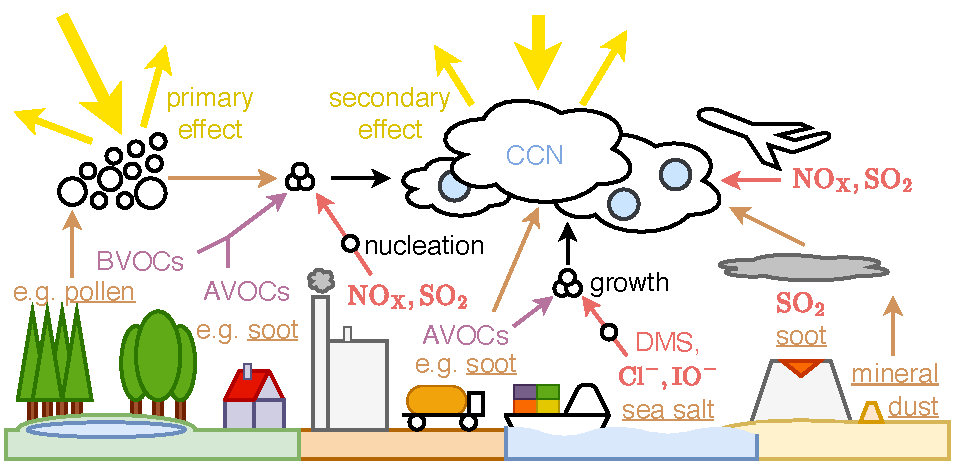
\includegraphics[width=0.9\textwidth]{background/figures/aerosols.pdf}
    \caption[Overview of the sources, formation process, and impacts of aerosols]{Overview of the sources, formation process, and impacts of aerosols. \textcolor{primary-aerosol}{\textbf{\underline{Primary aerosols}}} are emitted directly, while \textcolor{aerosol-precursor}{\textbf{precursors}} form \textbf{secondary aerosols} that can then grow with oxidised \textcolor{aerosol-voc}{\textbf{VOCs}} into \textcolor{aerosol-ccn}{\textbf{Cloud Condensation Nuclei}}. Note that $\approx 55\%$ of \textcolor{aerosol-ccn}{\textbf{CCN}} come from \textcolor{primary-aerosol}{\textbf{\underline{primary emissions}}} and $45\%$ from \textbf{secondary aerosols} \cite{ccn-sources-2009}. Aerosols have health, visibility, and \textcolor{aerosol-climate}{\textbf{primary and secondary climate effects}}.}
    \label{fig:aerosol-emission-effects}
\end{figure}

\noindent Aerosol particles also impact our climate. They have a direct radiative forcing effect on the energy balance of the atmosphere as they scatter (and absorb) light and thus mostly\footnote{Black carbon, on the other hand, is an aerosol that contributes to global warming \cite{ipcc-6-summary-2021}.} reduce some of the sun-driven warming of the Earth. Additionally, aerosols also impact the formation of clouds\footnote{While aerosols also impact cloud dynamics, these are out of scope for this summary.}. The (cloud) droplets that clouds consist of do not form from just water molecules alone, as the air is not saturated enough by water in the atmosphere to initiate homogeneous nucleation \cite{ccn-1999}. Instead, ice particles/nuclei (IN) or \textbf{Cloud Condensation Nuclei} (\textbf{CCN}), which are aerosols in the Aitken and accumulation modes, are needed so that the water vapour can deposit or condense on them and form ice crystals or cloud droplets, respectively. If more CCN and IN are produced, the water in the atmosphere is distributed across more nuclei on which it can condense. Thus, more but smaller cloud droplets are created, which in turn increases the lifetime of clouds and reduces the intensity of rain. Furthermore, clouds with more and smaller cloud droplets scatter more light and have a higher albedo and thus reflect light more efficiently. Therefore, the overall net effect of aerosols is estimated to be cooling, even though some aerosol interactions, such as black carbon emissions, have warming effects \cite{ipcc-6-summary-2021}. However, the extent of this cooling effect is still unclear, and aerosols are the among the largest sources of uncertainty in the IPCC reports that aim to predict the extent of future global warming \cite{ipcc-6-summary-2021}.

\section{An Introduction to the SOSAA Model} \label{txt:sosaa-model}

Modelling atmospheric chemistry is essential to understand the impacts that anthropogenic emissions and our changing environment have on human health and climate change. Complex processes such as surface emission fluxes, turbulent transport, meteorology, aerosol formation, dry and wet deposition, and chemical reactions interact in the atmospheric boundary layer (ABL), which starts from the Earth's surface and can reach up to several kilometres \cite{sosa-description-2011}. However, many aspects of especially aerosol processes are still unknown and the subject of ongoing research. The complexity of simulating these interacting processes requires choosing between (a) simulating a small box volume for a short time at a high level of detail or (b) applying broad simplifications so that an approximate chemistry scheme can be simulated inside a global weather or climate simulation.

\newpar SOSAA, the model to \textbf{S}imulate \textbf{O}rganic vapours, \textbf{S}ulphuric \textbf{A}cid and \textbf{A}erosols, is a chemistry transport model that was originally implemented in \textcite{sosa-description-2011} ``to reconstruct the emissions, transport and chemistry in the ABL [atmospheric boundary layer]'' \cite{sosa-description-2011} around the Finnish measurement station SMEAR II at Hyyti\"al\"a \cite{smear-station-2013}. It models the atmospheric processes inside a one-dimensional height column, which starts from the Earth's surface and reaches up to a height of a few kilometres, using several box models stacked on top of each other. Each box simulates its internal processes independently for a given time step, after which turbulent mixing drives the chemical transport between the boxes and exchanges species concentrations. Then, the procedure is repeated for the next time step. Given the reduced 1D dimensionality of the model, SOSAA ignores both horizontal and vertical advection and thus works best in open, flat, and horizontally-homogeneous terrain, e.g. the boreal forest around Hyyti\"al\"a. \Cref{fig:sosaa-overview} shows the modules SOSAA consists of, which are implemented in Fortran and coupled by the meteorology that controls the chemical exchange.

\newpar Since its original implementation in \textcite{sosa-description-2011}, SOSAA has been continuously improved and applied in various studies, including \cite{sosaa-description-2014, sosaa-bvoc-2017, sosaa-ozone-2017, sosaa-trends-2021}. The simulation uses MPI, the Message Passing Interface, to parallelise the computation of the chemical kinetics and aerosol processes in different boxes. In contrast, the emissions, deposition, meteorology, and mixing of chemical species are serialised. SOSAA is highly customisable and supports changing the number and spacing of the height column of boxes (usually around $50$ boxes reach up to $3 \text{km}$), the time steps of different modules (usually the meteorology uses $\Delta t = 10 \text{s}$ while all other modules run at a lower frequency and $\Delta t = 60 \text{s}$), and toggling which atmospheric processes are included in the simulation.

\begin{multicols}{2}
    \begin{figure}[H]
        \centering
        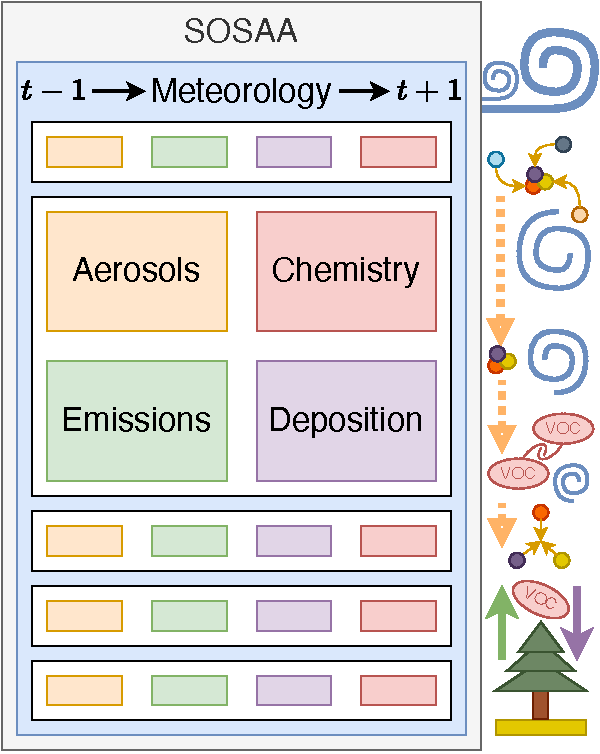
\includegraphics[width=0.49\textwidth]{background/figures/sosaa.pdf}
        \vspace{-1em}
        \caption[Overview of the Modules of the SOSAA Model]{Overview of the modules of the SOSAA model. SOSAA consists of a 1D stack of boxes that simulate emissions, deposition, chemical kinetics and aerosol processes. They are coupled through the meteorology.}
        \label{fig:sosaa-overview}
    \end{figure}

    \begin{enumerate}
        \item The \textbf{meteorology} module is a 1D version of the coupled plant-atmosphere boundary layer model SCADIS \cite{scandis-model-2002, scandis-analysis-2005, scandis-drag-2006}, which provides chemical mixing and transport between the thus-coupled boxes \cite{sosa-description-2011} and includes the ``prognostic equations for the horizontal wind vector, air temperature and absolute humidity'' \cite{sosaa-trends-2021}. In trajectory mode, global weather simulation outputs are used instead.
        \item The \textbf{emissions} module is a modified version of the MEGAN 2.04 \cite{megan-model-2006} model that provides plant canopy BVOC emissions, which are supplemented by governmental emission inventory data.
        \item SOSAA uses a chemistry reaction mechanism based on MCMv3.3.1 \cite{mcm-protocol-1997, mcm-v3-2003, mcm-beta-2012} for its \textbf{chemical kinetics}. The mechanism, which is compiled to Fortran using KPP \cite{kpp-preprocessor-2002}, simulates the time evolution of chemical species concentrations independently for each box model.
        \item Initially, the UHMA \cite{uhma-model-2004} model was used to simulate \textbf{aerosol} nucleation, condensation, coagulation and deposition processes. It is currently being replaced by the ARCA box model \cite{arca-box-2022}.
        \item \textcite{sosaa-bvoc-2017} added a multi-layer gas-\textbf{dry deposition} module \cite{gas-exchange-2002} to investigate the effect that not modelling the forest canopy as just one big leaf has on the atmosphere-biosphere gas-exchange and canopy gas-concentrations \cite{sosaa-bvoc-2017, sosaa-ozone-2017}.
    \end{enumerate}
\end{multicols}

\noindent The initial implementation of SOSAA only supported a stationary mode where the column of boxes remains in one location. In this mode, SOSAA models the nearby atmospheric processes for a measurement station like SMEAR II at Hyyti\"al\"a \cite{smear-station-2013}. Since long time series of high-quality measurement data are available at the station to constrain models, SOSAA has been used to simulate long-term trends in $\text{OH}$, $\text{NO}_3$ and $\text{H}_2\text{SO}_4$ concentrations at Hyyti\"al\"a \cite{sosaa-trends-2021}. More recently, a Lagrangian trajectory mode has been under development. In this mode, the trajectories of air parcels arriving at a measurement station are first calculated backwards in time, e.g. using FLEXPART \cite{flexpart-validation-1998, flexpart-correction-1999, flexpart-6.2-2005, flexpart-10.4-2019}. Next, the emissions and meteorological conditions along this trajectory are gathered from global weather models and emission databases. Finally, SOSAA is run along the trajectory by moving the box column to follow the path from the particle origins to the measurement station destination. Throughout, SOSAA is given the local meteorological conditions and the local aerosol, anthropogenic, and biogenic emissions. Whereas the stationary mode can use high-resolution and high-quality local measurement data, the trajectory mode often needs to interpolate more coarse data sources along the trajectory. Thus, the accuracy of some locally available variables is traded for new insights that the Lagrangian trajectory mode can give on far-away emission sources and the transport of aerosols and chemicals.

\newpar All SOSAA model runs for this thesis were performed with \href{https://version.helsinki.fi/putian.zhou/sosaa/-/tree/10618aa98c7470546308adf132afb0bc0735b4eb}{SOSAA@10618aa}. A snapshot of this now-outdated version can be accessed at \href{https://doi.org/10.5281/zenodo.7867026}{doi:10.5281/zenodo.7867026}. Unfortunately, the SOSAA model is not yet generally publicly available. However, access to the complete SOSAA source code is provided upon request -- please contact Michael Boy (\href{mailto:michael.boy@helsinki.fi}{michael.boy@helsinki.fi}), Putian Zhou (\href{mailto:putian.zhou@helsinki.fi}{putian.zhou@helsinki.fi}), or Petri Clusius (\href{mailto:petri.clusius@helsinki.fi}{petri.clusius@helsinki.fi}) for more information.

\section{A brief Introduction to Machine Learning} \label{txt:machine-learning}

Machine Learning is a field of research that investigates and develops methods that learn new behaviours by being shown examples of the behaviour and receiving feedback on their performance. More formally, \textcite{machine-learning-1997} gives the following definition:
\begin{center}
    ``A computer program is said to \textbf{learn} from experience $E$ with respect to some class of tasks $T$ and performance measure $P$ if its performance at tasks in $T$, as measured by $P$, improves with experience $E$.''
\end{center}
For instance, machine learning can train a smartphone camera to detect faces in an image. In this case, the \textbf{task} is to identify which rectangular areas in an image contain faces. To \textbf{train} the camera for this task, it is shown images that contain faces. The more images it is shown, the more \textbf{experience} the algorithm has with detecting them. Often it is also informed about the true locations of all faces in all images. Finally, the detection algorithm's \textbf{performance} is \textbf{evaluated} by calculating a punishment score, called the loss function $\mathcal{L}$, that increases the further away and differently sized each predicted face is from each actual face location.

\newpar Machine Learning is part of the broader academic discipline of Artificial Intelligence \cite{ai-review-2008}, which also encompasses fields such as genetic algorithm optimisations, logic-based reasoning, knowledge representation, and artificial life. Machine Learning combines ideas from data science, mathematical fields like statistics, as well as algorithms and computational methods from computer science. Insights from the natural sciences also often inspire progress in machine learning \cite{biological-dnn-2021}. Given this diversity of backgrounds in machine learning, it is imperative to define the terms, notations, and symbols that this thesis uses:
\begin{enumerate}
    \item \textbf{Variables} are represented with one letter, e.g. $X$ or $y$. Lowercase letters refer to vectors, while uppercase letters represent matrices. For instance, a dataset $X$ of face positions contains many rows $x$, each encoding example of a face. The columns of the dataset encode the face's features, e.g. its image location.
    \item A machine-learning \textbf{algorithm} or \textbf{method} refers to the description of how to construct, train, and evaluate a machine to learn a certain task. In contrast, a machine-learning \textbf{model} is an instance of a method. While a method is designed by a human, a model is trained by the machine to improve its performance on its given task. A model's tunable configuration options are called its trainable \textbf{parameters}, while the method's options are referred to as \textbf{hyperparameters}.
    \item Different tasks often require different Machine Learning paradigms. In \textbf{supervised} learning, a model is trained by being given examples of both the \textbf{input} and \textbf{target output} for the specific task. In contrast, an \textbf{unsupervised} model is trained with only the inputs. The third machine learning paradigm is \textbf{reinforcement} learning, where the model actively explores the input space, decides which action to take, and is rewarded or punished according to its performance.
    \item Supervised models are trained with a \textbf{training} set $(X_{\text{train}}, Y_{\text{train}})$ that contains pairs of input-output examples $(x, y)$. The columns of the input are called \textbf{features}, while the rows are often called \textbf{samples}, \textbf{examples}, or \textbf{points}. Some methods use a separate \textbf{validation} set $(X_{\text{valid}}, Y_{\text{valid}})$ to further finetune a model after training. Finally, the model is tested on the inputs for a \textbf{test} set $X_{\text{test}}$. The model's predictions for the target output, denoted as $\hat{Y}$, are then compared to the \textbf{true} target outputs $Y_{\text{test}}$ to evaluate the model's performance. Thus, the goal of a supervised model is to learn the process $f(X) = Y$ behind the training data and approximate the outputs with its predictions $\hat{Y} \approx Y$.
    \item \textbf{Regression} models predict continuous outputs. In contrast, \textbf{classification} models learn to predict one (single-class) or more (multi-class) options from a fixed set of discrete output \textbf{classes}. Both regression and classification are examples of supervised learning methods.
\end{enumerate}

\noindent This section provides a brief and targeted overview of a few machine learning methods. In particular, \Cref{txt:linear-model} introduces the Classical Linear Regression Model and the assumptions it is built upon. Next, \Cref{txt:data-preprocessing} highlights how the training data can be preprocessed to support the learning process. \Cref{txt:bootstrapping} and \Cref{txt:ensembles-decision-tree-random-forest} continue by introducing bootstrapping and ensemble methods, which are demonstrated with the example of decision trees and random forests. Following on, \Cref{txt:padre-rf} reviews the Pairwise Difference Regression method that is designed to make robust predictions even with little training data. Next, \Cref{txt:neural-network} provides the brief background on neural networks that this thesis requires, while \Cref{txt:auto-differentiation} dives deeper into the topic of automatic differentiation. Finally, \Cref{txt:ml-libraries} introduces the machine-learning libraries that are used in this thesis. Please refer to \textcite{machine-learning-1997} for a more comprehensive introduction to machine learning.

\subsection{The Classical Linear Regression Model} \label{txt:linear-model}

The classical linear regression model is one of the simplest machine learning models. It attempts to fit a linear relationship between a set of $k$ independent input variables $X_1, ..., X_k$ and the output variable $Y$ by tuning the model intercept or bias $b$ and the regression coefficients $a_1, ..., a_k$ \cite{clrm-assuptions-1971}:
\begin{equation}
    Y = \sum_{i=1}^{k}{(a_i X_i)} + b + \epsilon
\end{equation}
where $\epsilon$ is an added error term that represents the effect of unknown input variables or inherent randomness in the system. Note that the bias $b$ is often integrated into the regression coefficients by introducing a new constant input $X_0 = 1$ and setting $a_0 = b$. The classical linear regression model should only be used to fit a dataset if the following assumptions about the input and output variables hold \cite{clrm-assuptions-1971}:
\begin{enumerate}
    \item \textbf{Non-random Input Measurements:} The values of the input-variables $X_1, ..., X_k$ are not stochastic, i.e. it is assumed that they were measured with zero or negligible error.
    \item \textbf{Linearity:} $Y$ is linearly related to the input variables $X_1, ..., X_k$.
    \item \textbf{Linearly Independent Inputs:} The input variables $X_1, ..., X_k$ are linearly independent, i.e. none can be expressed as a linear combination of the others.
    \item \textbf{Normal Error:} $\epsilon$ is normal distributed with zero mean.
    \item \textbf{IID Error:} $\epsilon$ is independently (no correlation between errors) and identically (the error distribution is constant across the input domain, i.e. homoscedastic) distributed.
\end{enumerate}

\noindent Clearly at least $k+1$ input-output pairs $(x_i, y_i)$ are required to fit the parameters $a$ of this linear model. However, since the error term $\epsilon$ is often not zero, e.g. because of randomness or missing inputs, identifying the exact solution is not possible in general. In that case, the ordinary least-squares solution $\hat{a}$, which minimises the squared error $(y_i-\hat{y}_i)^2$ between the prediction $\hat{y}_i$ and the true $y_i$, can be found for $N$ pairs \cite[P/mlr-ols]{stats-proofs-2022}:
\begin{equation}
    \begin{split}
        \hat{a} &= \argmin_{a}{\sum_{i=1}{N}{\left( a \cdot x_i - y_i \right)^2}} \\
                &= {\left( X^{\intercal} X \right)}^{-1} X^{\intercal} Y
    \end{split}
\end{equation}
where $X$ and $Y$ are the input data and output variable matrices. To avoid overfitting on noisy samples, it is recommended to fit the model on more than the required $k+1$ input-output pair training samples.

\subsection{Preprocessing Data for Effective Machine-Learning} \label{txt:data-preprocessing}

Many machine-learning algorithms are not `off-the-shelf' but require hyperparameter tuning of the method or preprocessing of the dataset \cite{statistical-learning-2009} to perform well\footnote{Random forests (see \Cref{txt:ensembles-decision-tree-random-forest}) require little tuning and are, thus, one notable `off-the-shelf' algorithm \cite{statistical-learning-2009, ml-hyperparameters-2021}.}. This subsection provides a very brief overview of different data preprocessing methods to improve a model's training process. Please refer to \textcite{data-preprocessing-2007} for a more extensive introduction to data preprocessing for supervised learning.

\newpar Input data can be of different kinds, including continuous and discrete quantitative features, or nominal and ordinal qualitative data \cite{feature-selection-2014}. However, when a given model does not support all of these datatypes, it is necessary to convert between them. For instance, ordinal features such as letter grades from \texttt{A} to \texttt{F} can be transformed into discrete integers or the continuous test score percentages associated with these marks. For nominal features, where no order of the set of inputs exists, the one-hot encoding transforms each value into a binary feature that indicates whether or not the specific value is present. Continuous inputs can also be discretised into a reduced range of statically or dynamically selected bins \cite{data-preprocessing-2007}.

The collected training dataset may also contain errors such as missing values and outliers with unexpectedly high measurement errors. Some methods, such as decision trees, can explicitly deal with missing values \cite{machine-learning-1997} and are robust to outliers \cite{statistical-learning-2009}. For other methods, however, it may be necessary to filter out outliers using novelty detection (see \Cref{txt:novelty-detection}) and replace missing values with the feature mean, mode, or the value that is most often observed with similar inputs \cite{data-preprocessing-2007}.

ML models learn through the evaluation of their performance on a training dataset. If they are trained on a skewed dataset that does not reflect the true input distribution, they often overfit on the skewed data and thus perform worse on minority inputs \cite{ml-bias-discrimination-2017}. In such cases, either stratified sampling or data reweighting should be used \cite{data-preprocessing-2007}. While stratified sampling finds a training subset in which the different outcomes are represented equally, reweighting gives minority samples higher weight such that all samples are used, and the model is forced to be more careful with minority inputs even though they are still underrepresented in the training data.

\newpar ML models are generally constructed for fixed-size inputs and outputs. However, input domains such as images can be of arbitrary sizes, and tasks such as detecting the locations of all faces in an image may require variable-sized output lengths. Fixed-sized models can be trained and applied to this data by only providing them with a fixed-size window view of the data that is shifted across the input and for which they then make a fixed-size prediction. To account for variations in scale, a pyramid of several increasingly large, typically increasingly downsampled windows can also be provided as input \cite{feature-pyramid-1984}.

Training a model on a high-dimensional dataset is often challenging as computational performance decreases with increasing dimensionality \cite{ml-pattern-2006}, noise increases, and the distances between inputs become more difficult to interpret. Therefore, reducing the input dimensionality is often beneficial and acts as a feature selector to remove redundant or unimportant features. Principal Component Analysis (PCA) is among the most popular linear dimensionality reduction methods. PCA identifies a new set of orthogonal basis vectors, the principal components, that best explain the variance in the data. In particular, if $k$ principal components have already been identified, the $k+1$ component is the one that explains most of the still unexplained variance \cite{pca-1901}. Thus, projecting the data onto the $k$ first principal components produces the $L_2$-norm-optimal linear dimensionality reduction into $k$ dimensions. Note that PCA can also be extended to non-linear dimensionality reduction, e.g. by first applying a non-linear transformation kernel to the data \cite{kernel-pca-1997}.

PCA is very sensitive to the scale of the input variables, which becomes problematic if different features have different units and scales. It is thus recommended to first standardise the input by subtracting each feature's mean and rescaling them to unit variance using $x' = (x - \text{E}[x]) \mathbin{/} \sqrt{\text{Var}[x]}$. Standardising features is not only helpful with PCA but also with many other methods. For example, many algorithms use regularisation as a method against overfitting \cite{statistical-learning-2009}, which often discourages learning large model coefficients. However, if different features are of very different scales, such large coefficients may be required to explain the data, and regularisation may thus make the learning process unnecessarily slow \cite{data-preprocessing-2007}. Normalising features using $x' = \frac{x - \min(x)}{\max(x) - \min(x)}$ is an alternative approach to transform all features to comparable ranges. If the inputs span several orders of magnitudes, it may be beneficial to first take the logarithm of the inputs before rescaling them. Alternatively, the cumulative distribution of the inputs can be approximated to transform the inputs into a percentile score.

In addition to feature selection, new features can also be constructed. For instance, polynomial expansion and non-linear transformations can be applied to the features of a linear regression model (see \Cref{txt:linear-model}) to allow it to fit non-linear processes. It is also often possible to manually construct new features using domain-specific background knowledge.

\newpar While this subsection has only given a brief overview of feature preprocessing, it still highlights the expansive scope of this topic and the available options. AutoML Methods such as Auto-WEKA \cite{automl-2013} or Auto-sklearn \cite{auto-sklearn-2019} have thus been developed to reduce the need for manual configuration of the entire data preprocessing pipeline.

\subsection{Estimating Errors with Bootstrapping} \label{txt:bootstrapping}

Machine Learning has increased in accessibility, performance, and popularity with the increase in big data and highly parallel compute performance \cite{ml-trends-2021}. Today, many machine learning methods require large datasets to train a model, and high-confidence analysis of their performance requires collecting statistics over large data samples. However, such large amounts of data are only sometimes available. Therefore, squeezing as much information as possible out of smaller datasets is beneficial.

\newpar \textcite{bootstrapping-1979} introduced the Bootstrapping method to compute any statistic for an unknown distribution using only a small independently and identically distributed (iid) sample from the population. In its most basic form, resampling with replacement is used to generate $M$ different resamples of size $N$ for the original dataset of size $N$. Next, the target statistic is calculated independently for each of the $M$ resamples. Finally, the $M$ different results are combined, and their distribution is reported. Even though only data from the original small sample is used, bootstrapping can estimate the population statistic with much higher quality than only calculating the statistic on the original sample would have achieved.

For example, say we have a small set of noisy ozone concentration measurements from an urban area. If we are only interested in the sample mean, we can simply average all measurement samples. However, in this case, we want to estimate the true mean ozone concentration and the uncertainty of this estimate. Therefore, we generate $M$ new synthetic datasets by resampling the measurements with replacement, i.e. some measurements are included multiple times in one synthetic dataset, while others are excluded. Next, we calculate the mean for each of these resamples and thus produce a distribution of all the calculated means. The true mean can then be approximated as the mean of all means $\{\hat{\mu}\}_{i}$. In a normal distribution, the samples within one standard deviation of the mean fall between the $15.9\%$ and $84.1\%$ quantiles of its cumulative distribution function. Thus, we can extract these two quantiles to report the $\pm 1\sigma$ error range of our estimate $\hat{\mu}'$ of the true mean:
\begin{equation*}
    \hat{\mu}' = {\text{E}[\hat{\mu}]}^{+(\hat{\mu}_{84.1\%} - \text{E}[\hat{\mu}])}_{-(\text{E}[\hat{\mu}] - \hat{\mu}_{15.9\%})} 
\end{equation*}
\noindent Consider another example where we have a set of points that appear to have been generated by a simple process and some noise, e.g. $f(x) = a \cdot x + b + \epsilon$. While simply fitting a linear regression model to this data sample can give us the sample estimate for the gradient $a$ and intercept $b$, we are again interested in estimating these parameters and their uncertainties for the larger population that the samples originate from. While simply resampling the set of points is possible, we can do even better using our assumption that a linear regression model explains our data well. In particular, we can fit the model on the original sample and record the error residuals between the predicted line and the samples. Next, we apply bootstrapping on the set of residuals to resample them, add them back onto the fitted line, and generate completely new sets of points. Finally, a regression model can be fitted to each of these datasets to find their $a$s and $b$s, which can then be reported as described above using both their mean and $\pm 1\sigma$ confidence interval.

\newpar Bootstrapping is not only limited to simple statistics, however. For example, when a neural network (see \Cref{txt:neural-network}) is trained, it is often optimised on the same data several times. To capture as much information from the original training data as possible, bootstrapping can be used to resample the training data on every training epoch. The same approach is also used when networks are optimised on smaller subsampled batches instead of the whole dataset, which can be computationally more efficient. Last but not least, bootstrapping can also help with training several instances of the same model on resamplings of the original training data. These resamplings can then provide an ensemble of slightly different predictions, which is covered in \Cref{txt:ensembles-decision-tree-random-forest}.

\subsection{Ensembles: from Decision Trees to Random Forests} \label{txt:ensembles-decision-tree-random-forest}

How can one tell apart apples, bananas, and oranges? Apples are often red, bananas are usually yellow, and oranges are generally orange. However, apples and bananas can also both be green, some apples are yellow, bananas turn brown, and red bananas and oranges both exist. What about their shapes? While apples and oranges are both round, bananas are distinctly crescent-shaped. By looking at the shape first, bananas can thus be distinguished. Amongst the round fruit, orange ones can be classified as oranges. However, further details, such as texture, would be needed to distinguish green, yellow, or red oranges from apples.

\newpar The development of such a hierarchical set of rules is also found in \textbf{decision trees}. Decision Trees are tree structures that make predictions on inputs by recursively traversing the tree structure from the root down to each input's associated leaf. At every node, an attribute of the input is checked to determine to which of the node's children the input belongs to. Decision Trees can most easily be applied to discrete input and output values \cite{machine-learning-1997}, e.g. the name of a fruit's colour and what type of fruit it is. Each leaf in a decision tree contains one or more training examples, which are combined to form a final prediction. For instance, the leaves in the fruit classification example above may use a majority vote to determine which fruit is most common in the round-and-orange leaf. Decision Trees can also be extended to continuous inputs and outputs. In this case, the leaf's prediction usually is the mean value amongst all training examples in this leaf.

The ID3 algorithm by \textcite{decision-trees-1986} is a fundamental algorithm to train a decision tree on a dataset with discrete-valued attributes. It is a greedy recursive algorithm that starts at the tree root with the full dataset $D$ and then repeatedly asks which attribute $A$ the data should be partitioned on to achieve the greatest information gain, i.e. the greatest reduction in entropy \cite{decision-trees-1986, machine-learning-1997}:
\begin{equation*}
    \begin{split}
        \text{Gain}(D, A) = \text{Entropy}(D) - \sum_{v \in \{ x_A \given (x, y) \in D \}}{\frac{|D_v|}{|D|} \cdot \text{Entropy}(D_v)} \quad &\text{where} \quad D_v = \{ (x, y) \given (x, y) \in D \land x_A = v \} \\
        \text{Entropy}(D) = \sum_{c \in \{ y \given (x, y) \in D \}}{\left( -p_c \cdot \log_{2}{p_c} \right)} \quad &\text{where} \quad p_c = \frac{|D_{y = c}|}{|D|}
    \end{split}
\end{equation*}
Once the split with the highest information gain has been identified, child nodes are added for each discrete attribute value, the dataset is partitioned into these nodes accordingly, and the procedure is repeated recursively on the child nodes. Note that information gain is only one of a range of possible split ranking functions. For instance, the gain ratio penalises splitting attributes that have many uniformly distributed values and which might thus seem like very distinctive features but may cause the decision tree to overfit \cite{decision-trees-1986, machine-learning-1997}:
\begin{equation*}
    \begin{split}
        \text{GainRatio}(D, A) &= \frac{\text{Gain}(D, A)}{\text{SplitInformation}(D, A)} \\
        \text{SplitInformation}(D, A) &= \sum_{v \in \{ x_A \given (x, y) \in D \}}{\left( -p_v \cdot \log_{2}{p_v} \right)} \quad \text{where } p_v = \frac{|D_{x = v}|}{|D|}
    \end{split}
\end{equation*}
where $\text{SplitInformation}(D, A)$ is the entropy of $D$ with respect to the values of the attribute $A$. To avoid selecting split attributes only because they mostly have the same value and thus low split information and a high gain ratio, \textcite{decision-trees-1986} suggest only choosing by the gain ratio on attributes with above-average information gain.

If all inputs are discrete-valued, an attribute that has already been used to split the dataset does not need to be considered for splitting in any descendent nodes. Continuous attributes can also be supported by dynamically identifying partitioning points that translate a continuous attribute $x$ into discrete attributes such as $x \leq 4.2$ and $x > 4.2$. Please refer to \textcite{continuous-tree-1992} for an introduction to how the optimal real-valued attribute threshold points can be found by testing a range of cleverly chosen thresholds.

\newpar While decision trees are highly capable and can ``represent any discrete-valued function defined over discrete-valued instances'' \cite[p.~76]{machine-learning-1997}, they can also suffer from overfitting on the training data. Even though trees can be pruned after training to improve their generalisability, constructing an entire forest with many trees is a much simpler approach. Random Forests, which were first introduced by \textcite{random-forests-1995}, use bootstrapping (see \Cref{txt:bootstrapping}) to train several independent decision trees on bootstrapped random resamples of the training dataset. Furthermore, bootstrapping is also applied to the attribute split selection, where only a random sample of the attributes is considered to greedily select the next split. In particular, \textcite{statistical-learning-2009} note that it is recommended to consider $\sqrt{F}$ of the $F$ features for classification problems and to have at least one example per leaf node, while only looking at $\frac{F}{3}$ features and requiring at least five examples per leaf for regression tasks. At prediction time, each decision tree makes an independent prediction, which are then aggregated using voting for classification and the mean for regression. Combining bootstrapping the dataset and its features and aggregating prediction results makes random forests more robust against overfitting than individual decision trees \cite{random-forests-1995}, even when the forest's hyperparameters are not explicitly tuned \cite{ml-hyperparameters-2021}.

\newpar Random Forests are an example of an ensemble method that trains a group of sub-models and then aggregates their predictions to improve their performance \cite{statistical-learning-2009, ensemble-learning-2020}. \textcite{ml-ensembles-2000} has identified ``the three fundamental reasons why ensemble methods are able to out-perform any single [model] within the ensemble'' \cite[p.~13]{ml-ensembles-2000}. First, if many different models can explain ambiguous observations equally well, combining them reduces the risk of choosing the single model that generalises the worst on unseen data. Second, each model may individually get stuck in a local optimum during optimisation. However, the combination of all submodels can escape some local minima and get closer to the global optimum. Third, while each method may not have sufficient complexity to represent the modelled process by itself, the model ensemble can represent more complex processes.

There are three main methods for constructing ensembles. Bootstrap aggregation (see \Cref{txt:bootstrapping}), also called \textbf{bagging}, uses bootstrapping to resample the dataset and train independent model instances of the same method on each of the resamples, whose predictions are then combined using voting or averaging. Bagging helps to reduce the variance of its submodels and can thus be used to avoid overfitting \cite{ensemble-overfitting-1995}. \textbf{Boosting} instead tries to reduce the bias of the ensemble by training the submodels sequentially. Each new submodel focuses on areas of the input domain where the already-trained models do not yet perform well \cite{statistical-learning-2009}. The combined prediction is then calculated as a weighted average over the submodel predictions. Since boosting ensembles have dependent members, boosting should only be applied when the base models already have low variance and are not prone to overfitting. Last but not least, \textbf{stacking} combines submodels that use different machine-learning methods. In addition to the submodels, a metamodel is trained that makes the final prediction based on each submodel's prediction. Stacking is thus closely related to model selection, but instead of only identifying which submodel performs best, it finds their optimal combination, thus leading to better predictions \cite{statistical-learning-2009}.

\subsection{Pairwise Difference Regression for Low-Data Tasks in Science} \label{txt:padre-rf}

How can a machine learning model generalise over a vast and complex feature space when only a few training examples are available? Augmenting the training data set is often used in tasks like image recognition or object tracking. For instance, an image can be cropped, rotated, scaled, or slightly damaged with noise without changing the target value that should be predicted. However, how can augmentation be achieved in scientific regression tasks, where cheaply inventing new data points with correct targets may not be possible?

\newpar \textcite{padre-rf-2021} present the \textbf{PA}irwise \textbf{D}ifference \textbf{RE}gression method PADRE, which builds on prior work by \textcite{pairwise-images-2018} of pairing training samples for augmentation. \citeauthor{padre-rf-2021} are motivated by predicting chemical properties such as a molecule's free energy, which are usually determined through \textit{very} computationally expensive yet approximate simulations. Since any single simulation has an unquantifiable error, several simulations are performed instead to calculate the difference between a new molecule and several known ones. Crucially, combining their different predictions somewhat cancels their errors. Inspired by this method from computational chemistry, the authors suggest training a model on the \textbf{differences} between molecules. In particular, given the training data set $\{ (X, Y)_1, (X, Y)_2, ... \}$, the model is now trained to predict the difference in output given a pair of inputs and their difference, i.e. $f(X_i, X_j, X_i - X_j) = Y_i - Y_j$ instead of $f(X_i) = Y_i$. Suppose the model is trained with all possible input pairs. Then, the number of training examples increases from $N$ to $N^2$, though it is worth noting that they still hold less information than $N^2$ ``normal'' independently and identically distributed (iid) samples. Nevertheless, the increase in inputs makes it more difficult for a machine-learning model to overfit on the small training dataset. At test time, an unseen data point $X_k$ is paired with every training point $(X_i, Y_i)$ to produce the final prediction $Y_k$:
\begin{equation*}
    Y_k = \frac{1}{N} \cdot \sum_{i=1}^{N}{\left(f(X_k, X_i, X_k - X_i) + Y_i \right)}
\end{equation*}
Unfortunately, training and testing on all input pairs also decrease the method's performance by a factor of $N$. Instead, a fixed-size random subsample of training points can be used (see \Cref{txt:bootstrapping}). Also, note that the pairwise input vector $X_i \bigoplus X_j \bigoplus (X_i - X_j)$, as chosen by the authors, is just one possibility. Another option, only using the difference between inputs, $X_i - X_j$, reduces the dimensionality of the input feature vectors but assumes that the output gradient is constant across the entire input space. In contrast, the matrix product $X_i \times X_{j}^{\text{T}}$ of both inputs includes the most information at the cost of a quadratic increase in features.

\newpar \citeauthor{padre-rf-2021} use Random Forests (see \Cref{txt:ensembles-decision-tree-random-forest}) as the base model for their PADRE-RF method since Random Forests are efficient to train, more robust to hyperparameter selection than Neural Networks \cite{ml-hyperparameters-2021}, and more robust to high-dimensional feature vectors than Gaussian Processes \cite{gp-dimensionality-2005}. The authors demonstrate that PADRE-RF outperforms a direct RF model on several datasets. They also utilise the spread of the predictions for each data point to measure the prediction uncertainty, which \citeauthor{padre-rf-2021} show to be correlated with the prediction error. The authors then utilise this uncertainty prediction to apply PADRE-RF in an active learning loop and select new training data that has high uncertainty under the current model.

\subsection{A Very Brief Introduction to Simple Neural Networks} \label{txt:neural-network}

(Artificial) Neural Networks are a biologically-inspired statistical machine learning method to approximate highly complex and non-linear functions. Neural Networks (NNs) are loosely inspired by our brains, where roughly one hundred billion neurons \cite{machine-learning-1997} communicate in a densely interconnected network of synapses. NNs attempt to replicate a simplified version of our natural neurons with artificial \textbf{neurons}, which are functions that take in signals from a range of input neurons and transform them into a single output signal that is used as input for other neurons. NNs are generally organised in layers, starting from the \textbf{input layer}, passing through an arbitrary number of internal \textbf{hidden layers}, to one or more \textbf{output layer}s. In each layer $l > 0$, $M_l$ denotes the number of neurons or units that are stacked in parallel. In a fully connected layer, all neurons take the outputs of all neurons in the prior layer $l-1$ as inputs. Each neuron can then be expressed as calculating the weighted sum over its inputs and applying a non-linear activation function $\phi(x)$ to the results \cite{rio-2019}:
\begin{equation*}
    z_{l, j} = \phi \left( \sum_{k=0}^{M_{l-1}}{w_{l,j,k} \cdot z_{l-1,k}} \right)
\end{equation*}
where $z_{l, j}$ is the output of the $j$\textsuperscript{th} neuron in the $l$\textsuperscript{th} layer, $w_{l,j,k}$ is the weighting factor for the input from the $k$\textsuperscript{th} neuron in the previous layer for $k \in 1, 2, ...$ . As in the Classical Linear Regression Model in \Cref{txt:linear-model}, this weighting factor also includes a bias term $b_{l,j} = w_{l,j,0}$ and sets $z_{l-1,0} = 1$. Note that $z_{0, j}$ represents the $j$\textsuperscript{th} feature of the input $x_j$ to the neural network and that $M_0$ is the input's dimensionality. To obtain a prediction, the neural network is evaluated in a layer-by-layer forward pass that eventually calculates the prediction as a non-linear activation of a weighted sum of the outputs of the penultimate layer. The network is fit to perform a specific task by optimising the weighting parameters, including the biases, of all neurons in the network.

\noindent Why should all hidden layers in a neural network use non-linear activation functions? While a linear activation function can be helpful to predict a real-valued output in a regression problem, a network with only linear activations effectively collapses into a single-layer neural network since ``the composition of successive linear transformations is itself a linear transformation'' \cite[p.~229]{ml-pattern-2006}. However, stacking many non-linear layers is what gives neural networks their capability to fit complex and non-linear processes since the network can build up increasingly higher-order features with each layer. For instance, multi-layer perceptrons (MLPs) are the simplest form of neural networks, consisting of three or more layers (including the input and output layers), all of which are fully connected. While MLPs were originally only built with perceptron units, some other simple but widespread activation functions that can also be used include \cite{activation-functions-2020, machine-learning-1997}:
\begin{enumerate}
    \item \textbf{Perceptron:} The sign function $\phi(x) = \text{sign}(x)$ is used to construct the perceptron unit, used in one of the oldest neural network architectures \cite{perceptron-1943}.
    \item \textbf{ReLU}: The rectified linear unit $\phi(x) = \max(0, x)$ is a cheap activation function with derivative $\phi'(x) = \max(0, \text{sign}(x))$. It turns off a few neurons for each input and thus produces sparse network activations.
    \item \textbf{Sigmoid}: The sigmoid function $\phi(x) = \frac{1}{1 + e^{-x}}$ maps unbounded inputs to the $[0; 1]$ range and is thus often used in the final layer to produce binary classification probabilities. Its derivative is $\phi'(x) = \phi(x) \cdot (1 - \phi(x))$.
    \item \textbf{TanH}: The hyperbolic tangent function can be expressed by scaling and shifting the sigmoid function: $2 \phi(x) - 1$. It maps unbounded inputs to the $[-1; 1]$ range and can thus be conveniently used in hidden layers to describe the propagation of negative and positive activations.
\end{enumerate}
\noindent How are neural networks fit to learn a task? As noted by \textcite{machine-learning-1997}, machine learning for a specific task requires a performance measure with which the network can be evaluated on a set of training data. In supervised machine learning, the performance measure is often defined through a loss function $\mathcal{L}(y, \hat{y})$ which compares the expected true output $y$ with the prediction $\hat{y}$ and assigns a penalty for mistakes. The network is then trained to minimise this loss function for its predictions $\hat{y} = m(x)$. In regression problems, two common loss functions are the mean squared error loss $\mathcal{L}_{MSE}$ and the mean absolute error loss $\mathcal{L}_{MAE}$ \cite{ml-pattern-2006, mae-rmse-2005}:
\begin{equation*}
    \mathcal{L}_{MSE}(D_{\text{train}}) = -\frac{1}{|D_{\text{train}}|} \sum_{(x, y) \in D_{\text{train}}}{(y - m(x))^2} \quad \quad \quad \quad \quad \mathcal{L}_{MAE}(D_{\text{train}}) = -\frac{1}{|D_{\text{train}}|} \sum_{(x, y) \in D_{\text{train}}}{|y - m(x)|}
\end{equation*}
In binary classification problems, where the true label $y$ is either $0$ or $1$, the binary cross entropy loss $\mathcal{L}_{BCE}$ is minimised instead \cite{statistical-learning-2009}:
\begin{equation*}
    \mathcal{L}_{BCE}(D_{\text{train}}) = -\frac{1}{|D_{\text{train}}|} \sum_{(x, y) \in D_{\text{train}}}{\left( y \cdot \log(f(x)) + (1-y) \cdot \log(1-f(x)) \right)}
\end{equation*}
\noindent Given a training dataset $D_{\text{train}}$ and a loss function $\mathcal{L}$, the gradient descent algorithm takes the gradient of the loss function with respect to all network parameters $w$ to find the change in parameters $\Delta w$ that produces the greatest reduction in the loss function, i.e. that optimises the network's parameters to reduce misprediction penalties. Once these per-parameter gradients are known, the weight parameters can be updated using $w := w - \eta \frac{\partial \mathcal{L}}{\partial w}$, where $\eta$ is a learning rate. The gradients are often averaged over a small random batch of samples or the entire training dataset to reduce their noise. This weight update is performed once for each training epoch, each of which represents one pass over the entire training data \cite{statistical-learning-2009}. If a neural network with sufficient capacity is trained long enough, it may start to `learn' the noise inherent in the training data sample and thus overfit. While regularisation methods attempt to limit how much detail the network can learn, encouraging it to prioritise underlying processes over noise, monitoring the prediction error on a validation dataset and stopping the training early when it no longer improves is another approach \cite{machine-learning-1997, statistical-learning-2009}.

Note that if the loss function is visualised as a landscape, the gradient descent algorithm continuously takes steps in the direction in which the landscape descends most steeply. However, if the optimisation starts in a depression surrounded by mountains, gradient descent is only able to find a local minimum, a common issue with complex non-convex learning problems. Therefore, more complex algorithms for updating the parameters and avoiding overfitting have been developed \cite{gradient-descent-overview-2017}.

\newpar How can the gradients of the loss function with respect to each of the network parameters be calculated efficiently? Using the chain rule of differentiation, $\frac{dy}{dx} = \frac{dy}{du} \cdot \frac{du}{dx}$, the gradient of the loss function can be decomposed into its gradient with respect to an output from the penultimate layer, and that output's gradient with respect to the parameter. While the first gradient can be derived from the definition of the current layer and its activation function, the second one can again be decomposed, leading to a repeated application of the chain rule. Thus, while inputs are propagated forwards through the network to make a prediction, loss gradients are propagated backwards from the output to the parameters in order to train the network. It is worth noting that the gradients of a neural network cannot only be used to optimise it. For instance, some adversarial methods use gradient ascent to find the smallest change in the input that has the most negative impact on the prediction loss. The fast gradient sign method (FGSM), for example, perturbs by the sign of the gradient to optimise the misprediction with respect to the the $L_{\infty}$ norm of the perturbation, e.g. of image pixels \cite{fast-gradient-2014}:
\begin{equation*}
    x' = x + \epsilon \cdot \text{sign} \left( \frac{\partial \mathcal{L}(x)}{\partial x} \right)
\end{equation*}

\noindent This subsection has provided a very brief and basic introduction to neural networks. However, it entirely skips more advanced network architectures such as increasingly deep \cite{deep-learning-2019}, recurrent \cite{recurrent-nns-2019} or convolutional neural networks \cite{cnn-1990, cnn-review-2022}. Thus, please refer to the provided citations for an overview of recent advances in neural networks. Following on, \Cref{txt:auto-differentiation} delves into how the derivatives used in optimising neural networks can be derived automatically directly from the code that describes the forward prediction pass through the network.

\subsection{The Power and Promise of Auto-differentiation} \label{txt:auto-differentiation}

Neural networks are generally fit by using gradient descent to update their parameters to minimise a loss function. How are these gradients computed? \textcite{adifor-1992} list four possible methods for deriving the derivative of a function implemented in code:
\begin{enumerate}
    \item \textbf{By-hand}: Manual derivation underpins all other methods but is inefficient and prone to human error.
    \item \textbf{Divided Difference}: Derivatives can be approximated by evaluating a function several times with small perturbations $\Delta x$, e.g. using the first-order one-sided forward difference $f'(x) \approx \frac{f(x + \Delta x) - f(x)}{\Delta x}$, or the second-order central difference $f''(x) \approx \frac{f(x + \Delta x) - 2 \cdot f(x) + f(x - \Delta x)}{(\Delta x)^2}$ \cite{finite-difference-2022}.
    \item \textbf{Symbolic}: Symbolic differentiation operates on the symbols in mathematical formulas and applies known rules of differentiation, e.g. the product rule $(f(x) \cdot g(x))' = f(x) \cdot g'(x) + f'(x) \cdot g(x)$. While easy to implement, this method can suffer from rapidly growing equations that are difficult to optimise. Furthermore, handling programmatic control flow, such as conditional branches or loops, is challenging.
    \item \textbf{Automatic}: Since any complex function, even with conditional control flow, is executed by the processor as a stream of elementary mathematical operations, the derivative of this instruction stream can be derived through repeated application of the chain rule $(f(g(x)))' = f'(g(x)) \cdot g'(x)$ or equivalently $\frac{dy}{dx} = \frac{dy}{du} \cdot \frac{du}{dx}$.
\end{enumerate}
\noindent Auto-Differentiation has the advantage of being similarly mechanical as the symbolic approach but also being capable of deriving the derivative for any code that has one. The derivatives can generally be computed in either forward / tangent mode or backward / adjoint mode. In \textbf{forward} mode, the chain rule is applied after every operation to track how the derivative of one input propagates through the code to the derivatives of all outputs. While this mode is easy to implement and very efficient if we are only interested in the derivatives with respect to one or very few inputs, it often requires more temporary variables and loops than the reverse mode \cite{adifor-1992}. In \textbf{reverse} mode, the program's control flow needs to be reversed to calculate how the derivative of one output has been influenced by the derivatives of all inputs. While this method scales better if there are many inputs and only the derivatives for one or very few outputs are of interest, the reverse mode has the added complexity of needing to play back through the computation of a function in reverse. If all instructions are replayed and all intermediary values recomputed, the runtime complexity is quadratic in the number of operations \cite{tapenade-autodiff-2013}. If one instead stores all intermediary results and some metadata on which branches and loops were taken, calculating the derivative has linear complexity but requires an additional linear amount of memory. In practice, checkpointing can be applied to infrequently store intermediary checkpoints and recompute all values in between. The forward and reverse modes can also be interleaved in a \textbf{hybrid} mode, which \textcite{adifor-1992} demonstrated to exploit the benefits of both efficiently.

How is auto-differentiation implemented? \textcite{autodiff-taxonomu-1991} provides a taxonomy of different auto-differentiation approaches. \textbf{Operational} auto-differentiation provides the most elegant approach, where auto-differentiation is implemented within the constructs of the source language itself, e.g. by overloading mathematical operators and functions for a new class. In this approach, code that is generic over numbers remains untouched, and auto-differentiation can be applied to any such code by simply using it with the new class. While operator overloading is efficient in forward mode, it has to keep track of additional bookkeeping data in reverse mode. Reducing the amount of bookkeeping data can be achieved through support from the compiler, which can perform dataflow analysis that exceeds the local scope of a single overloaded operator. \textbf{Extensional} tools such as Adifor \cite{adifor-1992} or Tapenade \cite{tapenade-autodiff-2013} are precompilers that analyse and transform the source code to make it calculate a function's derivatives alongside its return value. They can thus use both the precompiler's knowledge of differentiation across function boundaries and the source language compiler's lower-level optimisations of the transformed source code. Finally, \textbf{integral} auto-differentiation refers to languages whose compiler directly supports auto-differentiation without any code transformation. Recently, \textcite{modeling-toolkit-2021} have introduced ModelingToolkit. This Julia library blurs the operational and extensional approaches by using operator overloading to build a symbolic representation of a function which is then transformed and compiled to support code transformations such as auto-differentiation, automatic parallelisation, or changing the algebraic complexity of an algorithm.

\subsection{Libraries for Machine Learning} \label{txt:ml-libraries}

As the popularity of machine learning has grown, a large number of libraries have been released to make it accessible yet also efficient for a broad audience. Python 3 \cite{python-3.7}, in particular, has become a popular language in research for exploring machine learning. This subsection provides a short overview of the Python libraries that are used in this thesis. Please refer to \textcite{python-ml-2020} for a broader overview of the data science, machine learning, and artificial intelligence ecosystem in Python.

\newpar The Scikit-learn library, \texttt{sklearn} for short, is an open-source Python library for accessibly exposing machine-learning to a non-specialist audience \cite{scikit-learn-2011} using a consistent and user-friendly API \cite{sklearn-api-2013}. \texttt{sklearn} builds on and integrates with existing scientific Python libraries such as \texttt{numpy} for vectorised calculations \cite{numpy-2020}, \texttt{scipy} for efficient scientific algorithm implementations \cite{scipy-2020}, \texttt{matplotlib} for visualisation \cite{matplotlib-2007}, and \texttt{pandas} for describing datasets as tabular data with named columns \cite{pandas-2010, pandas-software-2020}.

The library's consistent API design allows the user to quickly evaluate various methods for machine-learning tasks, including classification, regression, clustering, dimensionality reduction, and data preprocessing. All models in \texttt{sklearn} implement an \texttt{Estimator} interface that is primarily defined by its \texttt{fit} method, which takes in the training data inputs \texttt{X\_train} and outputs \texttt{y\_train} and returns the now-fitted model. Importantly, no configuration of the model algorithm via hyperparameters happens in the \texttt{fit} method. Instead, these hyperparameters are passed into the model constructor before \texttt{fit} is called. This concise API design allows scientists to easily swap out and compose models during research.

While \texttt{sklearn} provides an extensive range of models, it has specialised in providing classical algorithms with sensible default options for medium-scale ML problems. Therefore, many recent advancements in neural networks (see \Cref{txt:neural-network}) are not included in the library, which instead sticks to the most basic implementation that can be primarily used for educational purposes. In combination, the library's compact and consistent API with sensible defaults and focus on models that cover many research applications have all contributed to the library's popularity in research. Case in point, the original \texttt{sklearn} paper by \textcite{scikit-learn-2011} has amassed more than 4,800 citations at the time of writing \cite{scikit-learn-2011}.

\newpar TensorFlow is an open-source library that focuses on large-scale machine learning problems and supports easy production deployment to a variety of heterogeneous hardware. The library, which was developed at Google and first released in 2015 \cite{tensorflow-whitepaper-2015}, primarily targets the development of neural networks, which are constructed as dataflow computation graphs that describe the forward pass through the network. Computations are performed on tensors, which represent multidimensional arrays with a similar API as \texttt{numpy} arrays \cite{numpy-2020}. While TensorFlow initially only supported static data flow graphs that have to be declared and compiled before they can be evaluated \cite{tensorflow-whitepaper-2015}, TensorFlow 2.0 has added support for dynamically interacting with the computation graph using eager execution, a feature that was popularised by the competing PyTorch library \cite{pytorch-2019}.

In TensorFlow, users can write tensor-based Python code that is automatically compiled into a computation graph which can then use auto-differentiation (see \Cref{txt:auto-differentiation}), e.g. to optimise a neural network's loss function using backpropagation (see \Cref{txt:neural-network}). In addition to its lower-level graph interfaces, TensorFlow 2.0 also integrates the Keras API \cite{keras-2015}, which provides two different interfaces to build up the dataflow graph for machine-learning models. First, users can describe the high-level data flow with a functional API, where a network is constructed by writing its forward pass as a sequence of data transformations. Second, Keras' network layer and model classes can also be subclassed to control the computation inside a layer more precisely and to add custom control flow to a model's training process. In combination, users can thus quickly prototype models with the functional API and its provided utility functions but also refine any behaviour using subclassing.

TensorFlow has also been extended to more specialised domains through companion and third-party libraries building on TensorFlow's computation graph execution infrastructure. For example, the TensorFlow Probability library, the successor to TensorFlow Distributions \cite{tensorflow-distributions-2017}, integrates probabilistic methods with tensor computations. It provides probabilistic distributions that can be fit using gradient descent, probabilistic layers for neural networks, and probabilistic inference techniques such as Monte Carlo methods. The GPFlow library is a further extension that implements Gaussian Process inference and composable kernels \cite{gpflow-2017, gpflow-2020}. By building on TensorFlow Probability, it provides a similarly simple API for constructing Gaussian Process models that use auto-differentiation in their optimisation methods and can scale to large datasets on heterogeneous hardware.

The PyTorch library \cite{pytorch-2019}, which is based on the C++ Torch library \cite{torch-2002}, is the primary alternative to TensorFlow but not used in this thesis. It was originally developed at Meta but moved to the open technology Linux Foundation in September 2022 \cite{pytorch-linux-2022}. In contrast to TensorFlow, PyTorch's focus has been on supporting machine learning research through simple, fully Pythonic and imperative building block APIs that give the user full control, e.g. on whether data is stored on the CPU or GPU, but which may require more initial setup.

\section{Response Surface Models for Efficient Analysis} \label{txt:response-surface-models}

Performing complex and data-intensive analysis, e.g. global sensitivity analysis that identifies the most influential process factors \cite{global-sensitivity-2015}, on a simulation, such as an atmospheric model, is often expensive if it requires evaluating the simulation a large number of times. In that case, the analysis may be too costly to employ on a regular basis. How could the simulation output gathering for the analysis be sped up?

\textbf{Response Surface Models}, RSMs, are reduced form models \cite{emission-rsm-2022} such as simple linear models (see \Cref{txt:linear-model}), higher-order polynomials, statistical distributions, random forests (see \Cref{txt:ensembles-decision-tree-random-forest}), or neural networks (see \Cref{txt:neural-network}), which can all be evaluated very efficiently. Fitting an RSM to a simulation can provide a simplified representation that can be evaluated much more efficiently, thus speeding up the analysis. Notably, RSMs are based on statistical model fitting instead of creating a new but faster simulation that operates on a lower level of theory. To achieve speed and sufficient accuracy, some RSMs only approximate the response surface of the simulation in a small subset of the input parameter space.

RSMs have long been used in atmospheric science, particularly for air pollution models \cite{emission-rsm-2022}. Decision-makers are often interested in evaluating the effect of urban planning changes on their citizens' health. However, fully simulating the spread of air pollution is computationally expensive and it is thus difficult to iterate over different designs and evaluate their impact quickly. An RSM can allow decision-makers to explore the impact that small changes to the system would have on air pollution when compared to a previously simulated baseline.

\subsection{A brief History of RSMs in Atmospheric Science} \label{txt:rsm-history}

We first provide a brief overview of the development history of RSMs, which expands upon the summary given by \textcite{emission-rsm-2022}. Please refer to their work for examples of non-RSM reduced-form models in atmospheric science. \textcite{rsm-epa-2006} first introduced their air quality RSM, called `RSM', which statistically models the non-linear relationship between emission inputs and the air quality response using a Gaussian Process model (see \Cref{txt:gaussian-process}). To construct this RSM, the authors fit the Gaussian process using 180 runs of the CMAQ air quality model \cite{cmaq-2006}. A decade later, \textcite{ersm-v1-2015} and \textcite{ersm-v2-2017} presented Extended RSM (ERSM) v1.0 and v2.0, respectively, which adds the inter-regional transport of aerosols to the RSM. The transport is now also split into local, regional, and inter-regional effects. Following on, \textcite{pf-rsm-2018} improved the performance by capturing non-linear relationships using polynomical functions in their pf-RSM:
\begin{equation*}
    \Delta C = \sum_{i=1}^{N} \theta_i \cdot (E_{\text{NO}_{x}})^{a_i} \cdot (E_{\text{SO}_2})^{b_i} \cdot (E_{\text{NH}_3})^{c_i} \cdot (E_{\text{VOCs}})^{d_i} \cdot (E_{\text{POAs}})^{d_i}
\end{equation*}
where $\Delta C$ is the change in concentration of a pollutant, $\theta_i$ is the coefficient of the $i$th polynomial term, $E_{\text{NO}_{x}}$ is the ratio change in $\text{NO}_{x}$ emissions, $a_i$ is an integer power, and POAs are primary organic aerosols. The pf-RSM method drastically reduces the number of simulation runs that are needed to fit the model, down from 180 in RSM \cite{rsm-epa-2006} to 40 recommended training samples in pf-RSM \cite{pf-rsm-2018}.

The fitting of these polynomials was further improved by \textcite{epf-rsm-2020} with Epf-RSM, which applies the hill-climbing optimisation method \cite{hill-climbing-2004} to identify which polynomial complexity is needed in each grid cell. The hill-climbing method starts from an initial guess and then tests if a small change results in an improvement. If so, the optimisation is continued from the improved guess. Otherwise, it reverts to the previous guess. In this case, the integer powers in the polynomial fit are iteratively tweaked to reduce overfitting. Another advancement was made in pf-ERSM-SL by \textcite{pf-ersm-sl-2020}, which tackles source apportionment of pollution changes. The authors first split emissions into sectoral contributions. Next, the emission change ratio is again split into many subintervals, whose small effects thus approximate the local sensitivity to changes in the sector's emissions.

\newpar Both \textcite{deep-rsm-2020} and \textcite{self-adaptive-rsm-2022} have recently applied machine learning to further improve the polynomial fit in pf-RSM with DeepRSM and Self-Adaptive-RSM, respectively. The neural network approach used in DeepRSM, which brings the number of required simulation runs down to two \cite{deep-rsm-2020}, is explored in further detail in \Cref{txt:deep-rsm}. In the Self-Adaptive-RSM method, two different techniques are applied to make pf-RSM more robust \cite{self-adaptive-rsm-2022}. First, the pf-RSM function is fit using stepwise regression \cite{stepwise-regression-2010}, a process where the set of input features that are used for prediction is selected iteratively. Forward stepwise regression starts by identifying the single feature which best predicts the output by itself, i.e. which has the lowest prediction error. Next, the other features are checked to find the one that would most improve the fit, as evaluated by a partial F-test \cite{self-adaptive-rsm-2022} such as:
\begin{equation*}
    S_{k+1} = S_k \cup \{ f_i \} \quad \text{where} \quad \argmax_{i} F_i \quad \text{where} \quad F_i = \frac{RSS_{S_k} - RSS_{(S_k \cup \{f_i\})}}{\frac{RSS_{(S_k \cup \{f_i\})}}{n - (|S_k| + 1 + 1)}}
\end{equation*}
where $S_{k+1}$ is the new selection of features, $f_i$ is the newly added feature, $F_i$ is the F-score for adding feature $f_i$ to $S_k$, $RSS_{S_k}$ is the sum of squared errors for the model using only the prior selection of features, $n$ is the number of samples in the training data, and $|S_k| + 1 + 1$ is the number of trainable parameters, including the intercept, in the model that includes the new feature. This partial F-test uses the null hypothesis that adding the new feature has no effect. If the F-score exceeds a given threshold, the null hypothesis is rejected since a significant reduction in the error is indeed observable. In the following steps of stepwise regression, additional features are added until none of the excluded features exceeds the threshold, but all included features do.

Second, \citeauthor{self-adaptive-rsm-2022} also test the proposed feature addition for collinearity at every step. Two or more features are collinear if they can be explained as a linear combination of each other. Since regression models struggle with collinear features \cite{regression-collinearity-1984}, a new feature is rejected if adding it would fail the collinearity tests. In that case, the F-test threshold is also increased to discourage adding additional features. Finally, the pf-RSM method is applied to the set of selected features. Overall, the stepwise feature selection process and excluding collinear features make the model more robust to overfitting and reduce its computational complexity.

\subsection{Less Training Data with Deep Response Surface Models (DeepRSM)} \label{txt:deep-rsm}

Fitting a response surface model (RSM) requires many training data points that usually come from a large number of simulation runs. However, the computational cost associated with collecting these training data runs and fitting the model only pays off if the resulting RSM is later evaluated repeatedly and thus avoids needing to conduct more simulation runs. So how could the required amount of training data be reduced? \textcite{deep-rsm-2020} observe that many air quality simulations operate on a spatial grid and use fixed time steps. Each grid cell in space and time simulates the same physical processes as all other cells at every time step. Thus, instead of fitting the RSM to the simulation's final outputs, it is more efficient to fit a smaller RSM on the inputs and outputs of each cell. Since a single RSM is fit on the data from all cells, the amount of training data available per simulation increases drastically, and the number of simulation runs required to fit the RSM decreases.

\newpar This concept is borrowed from convolutional neural networks (CNNs), which we briefly describe in this paragraph. CNNs are biologically-inspired shift-invariant networks with a fixed-size footprint that are trained over arbitrary-sized input images by shifting the network over each image \cite{cnn-1990}. The shifting is achieved through convolutional layers, which use convolution instead of matrix multiplication to calculate the layer's outputs \cite{neocognitron-1980}. Downsampling layers that progressively increase CNN's receptive field, i.e. the area of inputs that affect each output, are in between some of the convolution layers. Overall, CNNs are characterised by sharing parameters across all shifts, which reduces the number of trainable weights and thus speeds up training and decreases the capacity for overfitting. While CNNs have their origins in 1980 \cite{neocognitron-1980}, they rose in popularity in the 2010s when advances in training neural networks on highly parallel graphics processing units (GPUs) enabled the AlexNet CNN architecture to win the prestigious ImageNet Large Scale Visual Recognition Challenge in 2012 \cite{alexnet-2017}.

\begin{figure}[H]
    \centering
    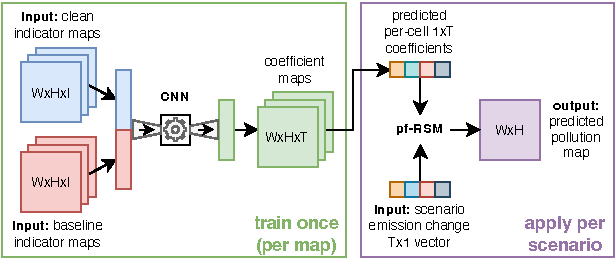
\includegraphics[width=0.9\textwidth]{background/figures/deep-rsm.pdf}
    \caption[Overview of the DeepRSM architecture]{Overview of the DeepRSM architecture, which trains a CNN to predict the parameters of a local, \textbf{T}-term-polynomial RSM, pf-RSM. Specifically, given the \textbf{W}idth$\times$\textbf{H}eight-sized concentrations maps for \textbf{I} indicators from a baseline and a clean simulation run, the CNN predicts the $1 \times$\textbf{T} per-grid-cell coefficients of the pf-RSM. These coefficients are then multiplied with a \textbf{T}$\times 1$-sized emission change input vector from an emission control scenario to produce the pollution concentration prediction map output. The CCN is trained to optimise these output predictions. Please refer to \textcite{deep-rsm-2020} for a detailed description of the layer-by-layer implementation of their CNN.}
    \label{fig:deep-rsm}
\end{figure}

\noindent \Cref{fig:deep-rsm} provides a high-level overview of the CNN-based DeepRSM architecture that \citeauthor{deep-rsm-2020} introduce. They build upon the polynomial RSM by \textcite{pf-rsm-2018}, pf-RSM, which is summarised in \Cref{txt:rsm-history}. However, \citeauthor{deep-rsm-2020} strive to fit the polynomial RSM using only the simulation runs for a ``normal'' baseline scenario and a clean air scenario. Note that while this choice drastically reduces the training collection burden, it also reduces the independence of the training data samples, which now only represent the chosen scenarios for a single area. With this reduced dataset, the authors train a deep CNN on the spatial concentrations of 18 indicator species to find the per-cell coefficients $\theta_i$ for the following pf-RSM-inspired polynomial:
\begin{equation*}
    \Delta C = \sum_{i=1}^{N} \theta_i \cdot (E_{\text{NO}_{x}})^{a_i} \cdot (E_{\text{SO}_2})^{b_i} \cdot (E_{\text{NH}_3})^{c_i} \cdot (E_{\text{VOCs}})^{d_i}
\end{equation*}
where $\Delta C$ is the change in concentration for a pollutant, $E_{\text{NO}_{x}}$ is the ratio change in in $\text{NO}_{x}$ emissions, and $a_i$ is a fixed integer power that is determined by the set of polynomial terms used for each pollutant\footnote{For instance, the following $N = 14$ polynomial terms are used to predict $\Delta |\text{O}_3|$: $\text{NO}_{x}$, ${\text{NO}_{x}}^2$, ${\text{NO}_{x}}^3$, ${\text{NO}_{x}}^4$, ${\text{NO}_{x}}^5$, $\text{VOCs}$, $\text{VOCs}^2$, $\text{VOCs}^3$, $\text{NO}_{x} \cdot \text{VOCs}$, $\text{NO}_{x} \cdot \text{VOCs}^3$, ${\text{NO}_{x}}^2 \cdot \text{VOCs}$, ${\text{NO}_{x}}^5 \cdot \text{VOCs}$, $\text{SO}_2$, and $\text{NH}_3$ \cite{deep-rsm-2020}.}. In the final layer of the CNN, the dot product between the learned coefficients $\theta_i$ and the emission change terms is taken to produce the pollutant concentration estimates. During training, the CNN is optimised with the following per-grid-cell loss function, which penalises high relative concentration errors between $y$ and $\hat{y}$ \cite{deep-rsm-2020}:
\begin{equation*}
    \mathcal{L}(\hat{y}, y) = \frac{||\hat{y} - y||_1}{y}
\end{equation*}
where $y$ is the simulated concentration $y$, and $\hat{y}$ the RSM prediction. At test time, the concentrations of the indicator species in a baseline and a clean run are passed through the CNN to predict the polynomial coefficients. The effect of a new emission control scenario is then obtained by taking the dot product of the emission change terms and the coefficients. After the CNN has been run on the indicator maps just once, the coefficients for this map can be stored, and any number of new emission control scenarios can be efficiently evaluated by a per-cell dot product. However, a change in the map requires a re-evaluation of the CNN.

\newpar \citeauthor{deep-rsm-2020} make three additional improvements to their deep CNN-based pf-RSM fitting procedure. First, they further increase the amount of training data by randomly cropping the simulation output maps. Second, the CNN is trained on batches of emission change vectors from different control scenarios. This batching ensures that the deep neural network has to generalise over several diverse scenarios at every gradient descent step. Third, the authors fit a three-layer fully connected neural network on the emission change vector to produce 50 additional polynomial factors that compensate for effects that the 14-term pf-RSM polynomial cannot capture. This extra `Compensated Polynomial Term' module thus also serves as an error predictor for the pf-RSM.

The authors demonstrate that their DeepRSM generalises well across different time spans and locations in the same simulation area. They also show that the pre-trained DeepRSM CNN can easily be adjusted for a new application area by retraining it with little new simulation data from the new domain. Thus, DeepRSM can indeed be successfully applied after training on just two simulation runs \cite{deep-rsm-2020}.

\subsection{Integrating Uncertainty with Stochastic RSMs} \label{txt:stochastic-rsm}

How can RSMs integrate the uncertainty of their inputs? \textcite{srsm-phd-1999} further extend RSMs to Stochastic RSMs, SRSMs, which take in random variables as inputs to propagate each input's uncertainty to the output. Similar to pf-RSM, a polynomial is fit to the data, though it is now a combination of random variables instead of observed values. In particular, the authors use a set of independent standard normal random variables $\text{N}(0, 1)$ to represent the uncertainties in all model input variables. Since the output of the SRSM is a polynomial combination of these random variables, the uncertainty in any prediction can be evaluated analytically on the SRSM's polynomial.

\newpar How is an SRSM fit to a model with non-normal-distributed input uncertainties? First, the input distributions are transformed into a set of independent standard normal random variables. For instance, the normal distribution $\text{N}(\mu, \sigma^2)$ and the uniform distribution $\text{U}(0, 1)$ can be obtained from $\text{N}(0, 1)$ as follows \cite{srsm-phd-1999}:
\begin{equation*}
    \text{N}(\mu, \sigma^2) = \sigma \cdot \text{N}(0, 1) + \mu
\end{equation*}
\begin{equation} \label{eq:srsm-uniform}
    \text{U}(a, b) = a + (b-a) \left( \frac{1}{2} + \frac{1}{2} \cdot \text{erf}\left( \frac{\text{N}(0, 1)}{\sqrt{2}} \right) \right)
\end{equation}
where $\text{erf}(z) = \frac{2}{\sqrt{\pi}} \int_{0}^{z}{e^{-t^2} \text{d}t}$ is the error function. \citeauthor{srsm-phd-1999} also provides similar derivations for the lognormal, gamma, exponential, Weibull, and extreme distributions. Continuous distributions with unknown analytical forms can be approximated to a desired accuracy as a weighted sum of several independent normal random variables instead. For empirical distributions where a histogram or its cumulative distribution function $g(x)$ is known, the inverse sampling method can be applied to transform the random variable \cite[p.~28]{rv-generation-1986}:
\begin{equation*}
    x = g^{-1}(u) \quad \text{where} \quad u \sim \text{U}(0, 1) \text{ which is obtained from N}(0, 1) \text{ using \Cref{eq:srsm-uniform}}
\end{equation*}
Since all previously described methods assume independent random variables, the authors also present a transformation for correlated random variables \cite[pp.~42-43]{srsm-phd-1999}, which is not further described here.

\citeauthor{srsm-phd-1999} use polynomial chaos expansion on the selected set $\{\text{N}(0, 1)_i\}_{i=1}^{N}$ of $N$ independent standard normal random variables. Polynomial chaos expansion \cite{polynomial-chaos-1938} refers to the ``series expansion of normal random variables, in terms of Hermite polynomials'' \cite[p.~44]{srsm-phd-1999}, which form ``an orthogonal basis for the space of square-integrable pdfs [probability density functions]'' \cite[p.~44]{srsm-phd-1999}:
\begin{equation} \label{eq:polynomial-chaos}
    \begin{split}
        y \approx a_0 &+ \sum_{i_1 = 1}^{N} a_{i_1} \Gamma_1(\xi_1) + \sum_{i_1 = 1}^{N} \sum_{i_2 = 1}^{i_1} a_{i_1,i_2} \Gamma_2(\xi_1, \xi_2) \\ &+ \sum_{i_1 = 1}^{N} \sum_{i_2 = 1}^{i_1} \sum_{i_3 = 1}^{i_2} a_{i_1,i_2,i_3} \Gamma_3(\xi_1, \xi_2, \xi_3) + ...
    \end{split}
\end{equation}
where $y$ is the simulation output that is being approximated, $a_1, a_{1,1}, ...$ are the coefficients whose values are to be determined during fitting, $\{ \xi_1, \xi_2, ..., \xi_N \}$ is the set of $N$ standard normal samples that are obtained from the simulation input $X$ through the aforementioned transformations, and ``$\Gamma_p(\xi_1, ..., \xi_p)$ are multi-dimensional Hermite polynomials of degree $p$'' \cite[p.~45]{srsm-phd-1999}, which are functions of random variables and thus random variables themselves. Please refer to \textcite{polynomial-chaos-1938} and \textcite{polynomial-chaos-1991} for a thorough introduction to polynomial chaos expansion and the Hermite polynomials.

The generated polynomial from \Cref{eq:polynomial-chaos} is fit using collocation, i.e. a system of linear equations is constructed that sets the polynomial equal to the simulation outputs at a set of collocation input points. These systems, which require one simulation result sample per coefficient to fit, can then be solved using any linear solver. For instance, fitting a second-order polynomial chaos expansion requires $N_2 = 1 + 2N + \frac{N(N-1)}{2} = \text{O}(N^2)$ samples, while a third-order expansion already needs $N_3 = 1 + 3N + \frac{3N(N-1)}{2} + \frac{N(N-1)(N-2)}{6} = \text{O}(N^3)$ evaluations to be fit. Since the collocation method finds a polynomial that exactly passes through all collocation points, it is sensitive to the selection of these reference points. The authors present a twofold solution to improve the stability of this process. First, they present a novel `Efficient Collocation Method', which picks collocation points that are closer to the zero-mean of the input standard normal random variables and thus have higher probability. Second, they propose generating twice the number of required samples and then finding the optimal but non-exact polynomial-coefficient solution for the now overdetermined system of linear equations. This fitting process is started with a low-order polynomial chaos expansion and repeated for increasing orders until some user-defined convergence criterion is met. \citeauthor{srsm-phd-1999} note that this general fitting procedure can also be optimised if more insight into the underlying simulation exists. While the process above works on any black box model, known linear transformations of the inputs can be translated analytically, and specific non-linear modules can then be fitted separately.

\newpar \citeauthor{srsm-phd-1999} also explore how the number of samples required to fit the polynomial chaos expansion can be reduced. If auto-differentiation (see \Cref{txt:auto-differentiation}) can be applied to the underlying simulation to automatically calculate the derivative of the simulation output with respect to $M$ simulation input variables, these derivatives can also be plugged into the collocation equations alongside the model outputs:
\begin{equation*}
    \begin{split}
        f(X_i) &= y_i \quad \forall i \in \{0; N\} \\
        \frac{\partial f(X_i)}{x_j} &= d_{i,j} \quad \forall i \in \{0; N\}, j \in \{0; M\}
    \end{split}
\end{equation*}
where $X_i$ is the input for a particular sample, $x_j$ is the $j$th component of the input vector, and $d_{i,j}$ is the partial derivative of the model output with respect to $x_j$ for the input $X_i$ as computed by auto differentiation. Thus, the number of data points per sample increases from $1$ to $1+M$, and the number of samples for the $k$th order polynomial chaos expansion decreases from $2N_k$ to $\frac{2N_k}{M+1}$. 

\textcite{srsm-2004} use the ADIFOR \cite{adifor-1992} auto-differentiation by source-code-transformation tool to fit an SRSM using both model outputs and derivatives. While Stochastic RSMs are built to describe how uncertainty propagates from the inputs to the output, they can also be used to reduce uncertainty. For example, in Bayesian inference, a model's parameter distributions are optimised by maximising the likelihood that this model with these parameters might have produced an observed output. If evaluating the likelihood function is expensive, it can be approximated with an SRSM to speed up inference \cite{srsm-2004}.

\section{Uncertainty Quantification for Model Predictions} \label{txt:uncertainty-quantification}

Machine Learning models are built to approximate often complex and non-linear processes. In most non-toy examples, these models make imperfect predictions. Furthermore, the prediction errors are usually not independently and identically distributed (iid) normal distribution samples from the same error distribution across the entire input domain. Simply trusting the model's point prediction or only reporting some globally-averaged error bounds are insufficient approaches to deal with prediction errors\footnote{If the uncertainty is homoscedastic, i.e. constant across the input space, global error bounds are sufficient. However, uncertainty is often heteroscedastic and varies across the input space.}. Knowing a model's uncertainty is especially relevant in domains where a model's predictions are safety-critical, such as medicine. \textbf{Uncertainty Quantification} is an expanding field in which more than 2,500 papers were published during the last decade \cite{uq-review-2021}. Since this section aims to give only a brief overview of a few methods relevant to this project, please refer to \textcite{uq-review-2021} for a broader review of the field.

\newpar In this section, we denote a model's input as $x$ and the target output it aims to approximate as $y$. Both can be scalars or vectors, but for now, they only represent one input-output sample each. A model with uncertainty quantification outputs two quantities. $\mu(x) \approx y$ is the model's point-approximation for the target output $y$. $\sigma^2(x)$ is the model's uncertainty prediction. If we assume that the model's prediction errors are Gaussian distributed, the model predictions follow the normal distribution $\text{N}(\mu(x), \sigma^2(x))$. However, uncertainty quantification can also be extended to non-normal-distributed errors, e.g. through observing the error distribution across an ensemble (see \Cref{txt:ensembles-decision-tree-random-forest} and \Cref{txt:mc-dropout}). Alternatively, several sub-models can be trained to predict the quantiles of the target function using the pinball loss \cite{regression-quantiles-1978, deep-quantiles-2022}:
\begin{equation*}
    \mathcal{L} = \begin{cases}
        q \cdot \mathcal{L}_{raw} \quad &\text{if } \mathcal{L}_{raw} \geq 0 \\
        (1-q) \cdot \mathcal{L}_{raw} \quad &\text{otherwise}
    \end{cases} \quad \text{where} \quad \mathcal{L}_{raw} = y - \hat{y}_{q}
\end{equation*}

\subsection{Predictive, Aleatoric and Epistemic Uncertainty} \label{txt:aleatoic-epistemic-uncertainty}

The error that a model makes can be quantified as its \textbf{predictive} uncertainty $\sigma^2(x)$. This predictive uncertainty consists of two parts, aleatoric and epistemic uncertainty:

\textbf{Aleatoric} uncertainty originates in the process from which the input data $x$ is sampled. It is thus often described as irreducible. Consider, for instance, modelling a chaotic system such as our weather. Both the measurements taken for model inputs and target outputs, and the physical processes that determine the system evolution contain some inherent randomness. Thus, the values of the inputs and the target output carry uncertainty that cannot be reduced and that any model must consider in order to avoid overconfident predictions.

\textbf{Epistemic} uncertainty, on the other hand, comes from the model's lack of knowledge about the process it is modelling. Continuing with the weather example, consider trying to fit a model with few training samples. While low-frequency patterns such as seasonal changes may be learned quickly, the day-to-day or hour-to-hour weather patterns may appear entirely random to the model if it lacks enough data points or variables to learn from. Therefore, several different models can come up with very different predictions, which signifies the ambiguity in how the model should be fit with this limited knowledge. In contrast to the irreducible aleatoric uncertainty, epistemic uncertainty can be reduced by providing a model with more training data, particularly in input regions where the output changes at high frequency.

\newpar How can a model's predictive errors be disentangled into aleatoric and epistemic uncertainty? Splitting the uncertainty is beneficial in several tasks. For instance, in active learning, a model's uncertainty for unseen inputs is used to evaluate for which inputs it would be most beneficial to find the true target outputs to extend the model's training set and improve its performance. However, collecting more training data in regions that are characterised by high aleatoric uncertainty would be of no use since this uncertainty is irreducible. On the other hand, regions of high epistemic uncertainty indicate that the model's predictions may be less trustworthy since it lacks essential knowledge about the processes it attempts to approximate.

\textcite{uncertainty-disentanglement-2022} provide a generalised method to disentangle aleatoric and epistemic uncertainty, which is based on prior work by \textcite{bayesian-deep-uncertainty-2017} for models using Monte Carlo Dropout (see \Cref{txt:mc-dropout}). For their method, the model needs to produce several estimates for its target output and uncertainty predictions. If the model is based on an ensemble (see \Cref{txt:ensembles-decision-tree-random-forest}) of sub-models, their target and uncertainty predictions $\mu_i(x)$ and $\sigma^2_i(x)$ can be taken. If the model is probabilistic, it can be evaluated several times to obtain the iid $\mu_i(x)$ and $\sigma^2_i(x)$ samples. The authors show that the combined predictive uncertainty
\begin{equation*}
    \sigma^2_{\text{predictive}}(x) = \frac{1}{N} \sum_{i=1}^{N} \left( \sigma^2_i(x) + \mu^2_i(x) \right) - \mu^2_{\text{predictive}}(x) \quad \text{where} \quad \mu_{\text{predictive}}(x) = \frac{1}{N} \sum_{i=1}^{N} \mu_i(x)
\end{equation*}
can be rewritten as
\begin{equation} \label{eq:uncertainty-disentanglement}
    \sigma^2_{\text{predictive}}(x) = \text{E}[ \sigma^2_i(x) ] + \text{Var}[ \mu_i(x) ] = \sigma^2_{\text{aleatoric}}(x) + \sigma^2_{\text{epistemic}}(x)
\end{equation}

\subsection{Cheap Uncertainty Predictions using Variance Attenuation} \label{txt:variance-attenuation}

How can a model be trained to cheaply output the uncertainty of its target value predictions? \textcite{nll-loss-1994} propose extending a neural network that predicts $\mu(x)$ with a second output for $\sigma^2(x)$. Since the prediction uncertainty is always positive and is never zero in real-world examples, they suggest using the exponential \cite{nll-loss-1994} or softplus \cite{reliable-variance-2019} activation functions, $\exp(x)$ and $\ln(1 + \exp(x))$ respectively, to impose these constraints. If the mean-squared error loss $(\mu(x) - y)^2$ is used to optimise the target value predictions, and a Gaussian prediction error distribution is assumed, the following \textbf{N}egative \textbf{L}og-\textbf{L}ikelihood loss $\mathcal{L}_{NLL}$ optimises the neural network to make the maximum likelihood predictions $y \sim \text{N}(\mu(x), \sigma^2(x))$:
\begin{equation} \label{eq:nll-loss}
    \mathcal{L}_{NLL}(x, y) = \frac{\ln(\sigma^2(x))}{2} + \frac{(\mu(x) - y)^2}{2 \sigma^2(x)}
\end{equation}
This loss function encourages low variance and accurate mean predictions, where possible, by down-weighting prediction errors with high variance. If the variance predictor captures aleatoric uncertainty well, down-weighting points with high aleatoric uncertainty can make the network training more robust to outliers \cite{bayesian-deep-uncertainty-2017}.

\newpar However, the variance attenuation loss $\mathcal{L}_{NLL}$ also has two problems. First, it is prone to overconfidence, i.e. predicting too-low variance \cite{reliable-variance-2019}. If the mean and variance predictor are trained together, the predicted variance is encouraged to approach zero since the target value predictions on the training data set keep improving \cite{variational-variance-2020}. However, since $\mathcal{L}_{NLL}$ in \Cref{eq:nll-loss} divides the prediction error $(\mu(x) - y)^2$ by $2 \sigma^2(x)$, minor prediction errors lead to large loss gradients when the predicted variance approaches zero, which makes the training process unstable. \textcite{reliable-variance-2019} propose, amongst others, two simple solutions to alleviate the overconfidence problem. Suppose the input dimensionality is low enough that the curse of dimensionality does not yet apply and nearest-neighbour distances are thus still meaningful. In that case, the authors suggest extending each training batch of $(x_i, y_i)$ pairs to also include the nearest neighbours of each $x_i$ to ensure that each batch contains information about both the target value mean and variance. Alternatively, training the mean and variance should be separated. After the network has been trained to predict $\mu(x)$ assuming constant predictive variance, the variance prediction is trained using the no-longer-updated mean predictions. This design also invites separating $\mu(x)$ and $\sigma^2(x)$ into two separate neural networks. Note that there are also more radical approaches to alleviate the variance overconfidence problem, including assuming Student's $t$ distributed errors \cite{reliable-variance-2019} or modelling variance variationally \cite{variational-variance-2020}, which are omitted here for brevity.

\newpar The second problem of the variance attenuation loss comes from its down-weighting of training samples with high predicted variance. While it is expected that the network may just predict the global mean value with high uncertainty during early training, there is the danger of the model getting stuck in such suboptimal predictions. In particular, if slightly more difficult points are always down-weighted, the model may never attempt to learn to predict them and thus perform much worse than a model trained only to output the target values but not the predictive variance. \textcite{beta-nll-2022} propose the following $\beta$-NLL loss to overcome this issue:
\begin{equation}
    \mathcal{L}_{\beta-NLL}(x, y) = \text{stop}(\sigma^{2 \beta}(x)) \cdot \mathcal{L}_{NLL}(x, y) \label{eq:beta-nll-loss}
\end{equation}
where $\beta \in [0; 1]$ is a newly introduced hyperparameter and the $\text{stop}(expression)$ function stops the gradient coming from the contained $expression$ from participating in the gradient backpropagation of the neural network (see \Cref{txt:neural-network}). As $\beta$ approaches zero, the $\beta$-NLL loss reduces to the original NLL loss. As $\beta$ approaches one, the gradient of the $\beta$-NLL loss with respect to the target value prediction $\mu(x)$ becomes equivalent to the gradient in the mean-squared error loss, where every training sample is given equivalent weight. The authors recommend $\beta = 0.5$ since it weights the samples with the ``inverse standard deviation instead of [the] inverse variance'' \cite{beta-nll-2022} and ``achieves the best trade-off between accuracy and log-likelihood'' \cite{beta-nll-2022}.

\subsection{Built-in Uncertainty with Gaussian Process Models} \label{txt:gaussian-process}

Gaussian Processes (GPs) are stochastic processes that fit a multivariate normal distribution to a training dataset. Specifically, GPs consist of a collection of random variables (RVs), where any linear combination of the RVs follows a multivariate normal distribution, e.g. $\mathcal{N}(\mu, \Sigma)$ \cite{gp-ml-2005}, where $\mu$ is the vector of per-variable means and $\Sigma$ is the inter-variable covariance matrix. It is important to note that this multivariate normal distribution can vary across different inputs $x$. A GP that represents a process $f(x)$ is denoted as \cite{gp-ml-2005}:
\begin{equation*}
    f(x) \sim \mathcal{GP}(m(x), k(x, x')) \quad \text{and} \quad f(x) \sim \mathcal{N}(\mu(x), \Sigma(x))
\end{equation*}
where $m(x)$ is the GP's mean function, $k(x, x')$ represents the GP's covariance, $x'$ is any input from the training data $X_{\text{train}}$, and $x$ is any input from the input domain. It is often assumed that the GP has zero mean and is thus only defined by its covariance. The covariance can be split into a covariance kernel $K(X, X)$ and observation noise $\sigma^2 I$. The kernel notation $K(X, X)$ is a shorthand for the matrix of pairwise covariances, where each entry $k_{i,j}$ is calculated using the function $k(x_i, x_j)$ \cite{rio-2019}. This thesis uses the following popular kernel functions:
\begin{enumerate}
    \item \textbf{Constant:} $k(x_i, x_j) = \sigma^2$
    \item \textbf{White Gaussian Noise:} $k(x_i, x_j) = \begin{cases}
        \sigma^2 &\quad \text{if } i = j \\
        0 &\quad \text{otherwise}
    \end{cases}$
    \item \textbf{Radial Basis Function (RBF):} $k(x_i, x_j) = \exp{\left( -\frac{||x_i - x_j||_2}{2 \sigma^2} \right)}$
    \item \textbf{Sum Kernel:} $k(x_i, x_j) = k_1(x_i, x_j) + k_2(x_i, x_j)$ where $k_1(x_i, x_j)$ and $k_2(x_i, x_j)$ are kernel functions
\end{enumerate}
\noindent When selecting the Gaussian Process kernel, knowledge about the problem domain can be used to compose a kernel that reflects the expected components of the real-world process. Next, the zero-mean GP is fit by optimising the log marginal likelihood of the covariance kernel. Finally, the fitted GP can be used to predict multivariate normal distributions for unseen inputs, where $\times$ denotes matrix multiplication \cite{gp-ml-2005}:
\begin{equation*}
    \begin{split}
        Y_{\text{test}} \given X_{\text{train}}, Y_{\text{train}}, X_{\text{test}} &= \mathcal{N}(\mu(X_{\text{test}}), \Sigma(X_{\text{test}})) \quad \text{where} \\
        \mu(X_{\text{test}}) &= K(X_{\text{test}}, X_{\text{train}}) \times [K(X_{\text{test}}, X_{\text{test}}) + \sigma^2 I]^{-1} \times Y_{\text{test}} \\
        \Sigma(X_{\text{test}}) &= K(X_{\text{test}}, X_{\text{test}}) - K(X_{\text{test}}, X_{\text{train}}) \times [K(X, X) + \sigma^2 I]^{-1} \times K(X_{\text{train}}, X_{\text{test}})
    \end{split}
\end{equation*}
\noindent By sampling from these predicted multivariate normal distributions $M$ times for a range of input points $x$, the evaluations of $M$ plausible \textit{functions} that explain the training data can be sampled \cite{gp-ml-2005}:
\begin{equation*}
    f_i(x) \sim \mathcal{N}(\mu(x), \Sigma(x)) \quad \text{where} \quad x \in X \text{ and } i \in \{1, ..., M\}
\end{equation*}
\noindent It is worth noting that prediction requires calculating the inverse of the covariance matrix, which has cubic complexity and is thus infeasible for large training datasets. Therefore, approximation methods are often used in practice. For instance, the training data set can be randomly or greedily \cite{gp-ml-2005} subsampled. More complex methods include Stochastic Variational GPs \cite{svgp-2013}, which use a reduced set of trainable inducing variables, and Actually Sparse Variational GPs \cite{asvgp-2023}, which project the GP onto a set of B-spline basis functions. Please refer to \textcite{big-data-gp-2022} for their classification and evaluation of GP approximation methods.

\subsection{Ensemble Uncertainty and Monte-Carlo Dropout} \label{txt:mc-dropout}

Predictive uncertainty can be decomposed into irreducible aleatoric uncertainty and model-based epistemic uncertainty (see \Cref{txt:aleatoic-epistemic-uncertainty}). Since aleatoric uncertainty is irreducible, several independent models should be able to measure it equivalently. In contrast, epistemic uncertainty describes the variation across different models that can explain the same observations with different theories but with equivalent accuracy. Put simply, epistemic uncertainty should be high if vastly different models can explain the data, and low if the models are forced to converge on a single hypothesis. Thus, it is intuitive to measure epistemic uncertainty as the spread of predictions across the models of an ensemble (see \Cref{eq:uncertainty-disentanglement}).

\newpar \Cref{txt:ensembles-decision-tree-random-forest} has already summarised why ensembles can make better predictions than the models they consist of \cite{ml-ensembles-2000}. Since ensembles thus provide benefits for both prediction and uncertainty quantification, ensembles have been extensively applied in recent years, e.g. \cite{mc-dropout-2016, deep-ensembles-2017, ensemble-uncertainty-2021, ensemble-diversity-2015, ensemble-uncertainty-ood-2021}. While this subsection provides a very brief overview of ensemble-based uncertainty quantification, please refer to \textcite{ensemble-uncertainty-2021} for a more extensive investigation of the topic.

\textcite{deep-ensembles-2017} introduce deep ensembles, which train an ensemble of neural networks (see \Cref{txt:neural-network}) with randomised initial parameter values and shuffled training data points. \textcite{ensemble-diversity-2015} have specifically highlighted the importance of diversity when training ensembles. They show that training over different random initialisations can be more potent than simply resampling the training dataset for each ensemble member. The authors also found that diversity is particularly advantageous in higher-level layers closer to the output. Thus, \citeauthor{ensemble-diversity-2015} introduced TreeNets as a compromise solution between fully independent and fully parameter-sharing ensemble members. TreeNets only share the first few neural network layers, followed by multiple distinct branches that make independent predictions.

Another approach, Monte Carlo Dropout by \textcite{mc-dropout-2016}, is based on dropout. Dropout was initially introduced by \textcite{dropout-2014} as a technique to reduce overfitting in neural networks. In particular, layers that use dropout randomly drop some of their outputs during training with probability $p$. Therefore, in every forward propagation through the network, only a fraction of the neurons are active, which leads to faster computation times for large networks. Furthermore, it forces the network to be robust to the failure of individual neurons, making it less likely to overfit. At evaluation time, no neurons are dropped, but all weights are multiplied by the factor $p$. Monte Carlo Dropout builds on this idea but also applies random dropout at prediction time. Since predictions are now random, the network can be sampled several times to obtain an ensemble of predictions and evaluate its uncertainty. \citeauthor{mc-dropout-2016} have shown that using Monte Carlo sampling on a network with dropout ``approximate[s] Bayesian inference in deep Gaussian processes'' \cite{mc-dropout-2016}.

% Andreas: Words with mathematical meaning should be defined on the first usage. Inconcise notation cannot be mixed with the use of mathematical properties lacking a concise definition. In addition, the mathematical citation style puts less emphasis on the author names.
\section{Avoiding Overconfidence using Novelty Detection} \label{txt:novelty-detection}

In machine learning, the closed-world assumption is generally assumed to hold. That is, a model's training data is assumed to be drawn independently and identically distributed (iid) from the same distribution as the test data and the data on which the model is later applied \cite{ood-boundary-2021}. Put simply, if we want a machine learning model to approximate some target function, the training data must cover \textbf{all} aspects of the possible input data sufficiently well. However, this assumption may not always hold.

\newpar For an easy and illustrative example, consider a model that is trained to distinguish between pictures of apples and bananas. However, during training, it is only shown pictures of green apples and pictures of yellow bananas. With such a limited training data set, the model might learn to associate apples only with the colour green, and bananas only with the colour yellow. What happens if the model is shown a red apple at test time? The closed-world assumption is clearly violated here since the model was never trained on red apples. Thus, the model might fail on this input in an unpredictable way and without any indication. This example is easy to catch: Since the model was never trained on any red fruit at all, it could refuse to make a prediction.

So what should the model do if it is shown a yellow apple and a green banana? Given its limited training, the model might mistake the apple for a banana and vice versa. Since the model has been trained on both apples and bananas and both the colours yellow and green, how could it have detected that it should not have made a prediction in this case either? During its training on the images of green apples and yellow bananas, the model likely observed both the colour and rough shape of each fruit but decided -- for simplicity -- to assume that all green fruit are around are apples and that all yellow fruit are crescent-shaped are bananas. When the model is then presented with a yellow but round fruit, the model's learned assumption that all yellow fruits are crescent-shaped is violated. If it can detect this assumption violation, the model can correctly determine that it should not make a prediction for yellow apples and green bananas.

\newpar To decide whether a model can make a prediction, one has to check whether a new input is similar to the inputs that the model was trained on. Inputs that the model was trained on are called \textbf{ID}, short for \textbf{in-distribution}, while inputs that come from a different distribution are called \textbf{OOD}, short for \textbf{out-of-distribution}. Deciding if an input is ID or OOD is an application of \textbf{novelty detection}. This machine learning task aims to identify novel inputs, anomalies, outliers, or exceptional data points amongst a set of ``normal'' data. As an unsupervised task, it is only presented with such ``normal'' ID data but no OOD examples during training \cite{novelty-detection-2010}. Thus, novelty detection can be phrased as a one-class classification problem \cite{ood-svm-1999}.

Novelty can occur at different scales \cite{novelty-detection-2010}. For example, a subset of data can be novel on a population scale if it follows a different distribution. Likewise, in a time series or a geographical map, individual data points can be novel in the context of their surrounding points. Such coarser-scale shifts in the data distribution can be identified using \textbf{concept drift} detection methods, which are discussed in further detail in \Cref{txt:concept-drift}. For individual points without context, however, an independent decision must be made for every single data point without being able to compare them to nearby points or population statistics. Building on the broad overview provided by \textcite{novelty-detection-2010}, the following subsections describe a variety of novelty detection methods in detail.

\subsection{A brief Overview of Concept Drift} \label{txt:concept-drift}

Before we dive into novelty detection methods for individual outlier points, we briefly summarise concept drift. Concept drift describes an unforeseen change \cite{concept-drift-definition-2019} in the distribution of input-output samples $(X, Y)$ across a contextual subsample, e.g. a period in time. Hence, concept drift deals with population-level changes in a distribution and does not consider individual outliers. Whereas individual-based methods can be applied to contextless individuals and data points from a population sample, concept drift methods only work on population samples. Thus, they can incorporate more information. For instance, a concept drift detector may not detect a single red apple amongst many green ones. However, it could detect if an apple's colour slowly changes from green to yellow over several images.

\newpar \textcite{concept-drift-definition-2019} formally define the existence of concept drift, which starts at a time point $t$ and spans a time window $w$, as
\begin{equation*}
    \exists t \st P_t(X, Y) \neq P_{t+w}(X, Y) \quad \text{where} \quad P_t(X, Y) \propto P_t(X) \cdot P_t(Y \given X)
\end{equation*}
where $P_t(X, Y)$ is the observed input-output distribution at time $t$, $P_t(X)$ is the input distribution at time $t$, and $P_t(Y \given X)$ is the output label posterior distribution given input $X$ at time $t$. This definition neatly distinguishes the three kinds of concept drift. \textbf{Virtual or feature drift} occurs when the input distribution $P_t(X)$ changes but the relationship to the output remains the same, e.g. when for a linear model $f(x) = 2x + 8$ the data samples shift from $\{ (1, 10), (2, 12), (3, 14) \}$ to $\{ (2, 12), (4, 16), (6, 20) \}$. \textbf{Real concept drift} occurs when the posterior $P_t(Y \given X)$ shifts but the input distribution remains the same, e.g. when $f_t(x) = 2x + 8$ changes to $f_{t+w}(x) = 3x + 8$ for the input distribution samples $\{ 1, 2, 3 \}$. Finally, both input and posterior distribution can also shift simultaneously. \textcite{concept-drift-rates-2014} further differentiate various concept drift types by the rate at which they occur. For instance, the drift can be abrupt, occur in incremental steps with intermediate concepts, gradually interpolate between the old and the new concept, or be recurring.

\newpar \textcite{concept-drift-detectors-2022} provide a comprehensive overview of the many proposed concept drift detection algorithms, which the authors classify into several categories. \textbf{Data-distribution-based} methods only observe the distribution of the input-output samples $\{(X_1, Y_1), (X_2, Y_2), ...\}$. These methods can further be restricted to only having access to the distribution of input samples $\{X_1, X_2, ...\}$. In that case, data-distribution-based methods can identify concept drift without needing access to the true output labels $\{Y_1, Y_2, ...\}$ or a machine learning model's predictions for the labels. \textbf{Performance- or error-based} methods instead monitor the prediction error of a model to determine when its performance no longer matches its training accuracy. While these methods, which can be based on model ensembles, comparison windows across time, or statistical significance tests \cite{concept-drift-detectors-2022}, only sound the alarm when a model actually starts to make consistent mispredictions, they \textbf{always} require access to the true output labels $\{Y_1, Y_2, ...\}$, which may not be available (yet). Finally, several detectors can also be combined in \textbf{hybrid} ensemble methods (see \Cref{txt:ensembles-decision-tree-random-forest}).

\subsection{A Baseline for OOD Detection in Classification} \label{txt:softmax-confidence}

Next, we discuss how the performance of an OOD input detector can be evaluated. \textcite{ood-baseline-2016} introduce a baseline method, which other OOD detection methods for classification can be compared against, and discuss which metrics should be used to measure their performance.

\newpar In classification tasks, the final layer of a neural network is usually a softmax activation function that scales the classification scores for each class into pseudo-probability scores that are non-negative and add up to one. For a specific class $c_i$ amongst all $N$ classes, the softmax activation $S_i(X)$ is defined for the input $X$ and the class scoring functions $f_i(X)$ as follows:
\begin{equation} \label{eq:softmax}
    S_{i}(X) = \frac{e^{f_i(X)}}{\sum_{j=1}^{N}e^{f_j(X)}}
\end{equation}
However, directly interpreting such softmax scores as classification probabilities often leads to highly overconfident predictions on out-of-distribution inputs, e.g. having $91\%$ confidence that Gaussian noise is an image of a particular handwritten digit \cite{ood-baseline-2016}. We further define the maximum softmax score as
\begin{equation} \label{eq:max-softmax}
    S_{c}(X) = \text{max}_{i} \{ S_{i}(X) \}
\end{equation}
i.e. the highest softmax score, or phrased differently, the score for the predicted class $c$. \citeauthor{ood-baseline-2016} show that this maximum softmax score $S_{c}(X)$ is more informative than an arbitrary $S_{i}(X)$, as the maximum score is usually lower for OOD inputs than for ID inputs. Put simply, classification models tend to assign ID inputs to one clear class but are more ambiguous for OOD inputs. The authors show that using a threshold to distinguish between ID and OOD inputs based on $S_{c}(X)$ thus performs well. They also present an auto-associative network-based abnormality detector as a first improvement to their method. Auto-associative networks are discussed in further detail in \Cref{txt:auto-associative}.

\newpar Like many other methods, the above baseline OOD detector relies on a threshold to distinguish between ID and OOD samples. \citeauthor{ood-baseline-2016} suggest using the threshold-selection-independent AUC-ROC and AUC-PR metrics to evaluate the performance of a detector method across all possible thresholds. Before introducing these metrics, the following commonly known terms need to be defined, here in the context of OOD detection:
\begin{enumerate}
    \item An OOD detector $d(X)$ classifies an input $X$ as either ID or OOD. For now, we designate OOD as a positive prediction and ID as a negative one, though the reverse is also possible.
    \item The \textbf{true positive rate} or \textbf{recall} $TPR = RC = \frac{|d(X_{\text{OOD}}) = \texttt{OOD}|}{|X_{\text{OOD}}|}$ is the percentage of actual OOD inputs that are correctly identified as OOD.
    \item The \textbf{true negative rate} $TNR = \frac{|d(X_{\text{ID}}) = \texttt{ID}|}{|X_{\text{ID}}|}$ is the percentage of actual ID inputs that are correctly identified as ID.
    \item The \textbf{false positive rate} $FPR = \frac{|d(X_{\text{ID}}) = \texttt{OOD}|}{|X_{\text{ID}}|}$ is the percentage of ID inputs that are mistakenly identified as OOD.
    \item The \textbf{false negative rate} $FNR = \frac{|d(X_{\text{OOD}}) = \texttt{ID}|}{|X_{\text{OOD}}|}$ is the percentage of OOD inputs that are mistakenly identified as ID.
    \item The \textbf{precision} $PR = \frac{|d(X_{\text{OOD}}) = \texttt{OOD}|}{|d(X_{\text{ID}} \cup X_{\text{OOD}}) = \texttt{OOD}|}$ is the percentage of OOD classifications that are correct amongst all ID and OOD inputs that are classified as OOD.
\end{enumerate}
Both the AUC-ROC and AUC-PR metrics calculate the \textbf{A}rea \textbf{U}nder the \textbf{C}urve of two metrics that the threshold has to find a trade-off for. For AUC-ROC, these are the true positive rate and the false positive rate. For AUC-PR, the precision and recall metrics are used instead, which \textcite{aucpr-informative-1999} deem to be more informative, e.g. when ID and OOD inputs are unbalanced. While AUC-ROC scores are independent of whether ID, or as above, OOD inputs are designated as positive, the AUC-PR scores are not and must be reported for both cases \cite{ood-baseline-2016}. \Cref{fig:auc-roc-pr} shows the AUC-ROC and AUC-PR curves for different classifiers. While a random detector obtains an AUC-ROC score of $0.5$, a perfect detector would get AUC-ROC and AUC-PR scores of $1.0$. The AUC-PR score of a random detector depends on the positive-negative class imbalance.

\begin{figure}[ht]
    \centering
    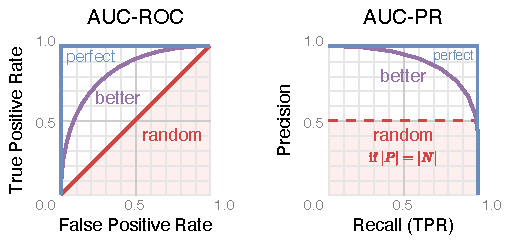
\includegraphics[width=0.9\textwidth]{background/figures/auc-roc-pr.pdf}
    \caption[Examplary AUC-ROC and AUC-PR score curves.]{Examples of AUC-ROC and AUC-PR score curves. While the AUC-ROC score of a random classifier is always $0.5$, the AUC-PR score depends on the rate of positive and negative examples.}
    \label{fig:auc-roc-pr}
\end{figure}

\noindent \textcite{odin-detector-2017} build on \citeauthor{ood-baseline-2016}'s baseline with their \textbf{O}ut-of-\textbf{DI}stribution detector for \textbf{N}eural networks, ODIN. They improve the softmax score with temperature scaling and anti-adversarially perturbed inputs to further push the softmax scores of ID and OOD inputs apart. In contrast to the softmax function as defined in \Cref{eq:softmax}, ODIN scales the scoring function outputs $f_i(X)$ by the inverse of a temperature parameter $T$: 
\begin{equation*}
    S_i(X; T) = \frac{e^{\frac{f_i(X)}{T}}}{\sum_{j=1}^{N}e^{\frac{f_j(X)}{T}}}
\end{equation*}
The $T$-dependent maximum softmax score is defined as $S_{c}(X;T) = \text{max}_{i} \{ S_{i}(X;T) \}$, following \Cref{eq:max-softmax}. The authors show that higher temperatures push ID and OOD scores further apart but that $T > 100$ brings no further benefits. To further increase the separation, \citeauthor{odin-detector-2017} suggest using the fast gradient sign method \cite{fast-gradient-2014} to perturb the inputs before feeding them through the classification network. Counterintuitively, they apply the FGSM to push an input \textbf{towards} its predicted class to increase the confidence in this prediction. Crucially, the authors observe that the increase in confidence is larger for ID than for OOD inputs. Both the temperature scaling and input perturbation are configured such that thresholding on the ODIN softmax scores achieves a true positive rate of $95\%$ on a held-out validation set that was not used during training.

\subsection{Distance-based Methods for Novelty Detection} \label{txt:ood-distance}

Intuitively, a machine learning model should perform well on inputs that are close to the inputs it was trained on. Several methods are built on this intuition to separate ID from OOD inputs. Many methods are based on the simple idea of constructing a bounding volume that includes most of the ID training data points. New inputs that lie on the inside of this volume are ID, while those on the outside are OOD. For instance, the Mahalanobis distance can be used to define a hyper-ellipsoid bounding volume by assuming that the ID data comes from a multivariate normal distribution \cite{mahalanobis-distance-1936, mahalanobis-outlier-2000}:
\begin{equation} \label{eq:mahalanobis-distance}
    d_{M}(x) = \sqrt{(x - \mu_{\text{ID}})^{\intercal} S^{-1}_{\text{ID}} (x - \mu_{\text{ID}})}
\end{equation}
where $d_{M}(x)$ is the distance between an input feature vector $x$ and the ID distribution, and $\mu_{\text{ID}}$ and $S_{\text{ID}}$ are the mean and covariance of the ID training data, respectively. Since the feature distances on the raw high-dimensional inputs are vulnerable to noise and difficult to interpret, the distances are often instead computed on higher-level and lower-dimensional embeddings, e.g. created by the upstream levels of a neural network.

\newpar \textcite{ood-adversarial-detection-2018} fit Gaussian mixture models (GMMs), i.e. weighted sums of multivariate normal distributions \cite{gmm-encyclopedia-2009}, to the training data embedding created by each layer. To classify an unseen input, they then select the class that the input is closest to based on their Mahalanobis distance. After perturbing the input's embedding in this layer adversarially away from the chosen class using the fast gradient sign method \cite{fast-gradient-2014}, the Mahalanobis distance is measured again and translated into a per-layer confidence score ${c}_{i}(x)$ that captures how well the input $x$ lies within the Gaussian fit of the class distribution in this layer. Finally, the parameters $\{ \beta_0, \beta_1, ... \}$ of a logistic regression model are fit on validation data to distinguish between ID and OOD inputs:
\begin{equation*}
    d(x) = \begin{cases}
        \texttt{ID} \quad & \text{if } s(x) < threshold \\
        \texttt{OOD} \quad & \text{otherwise}
    \end{cases} \quad \text{where} \quad s(x) = \frac{1}{1 + e^{-(\beta_0 + \sum_{i}\beta_i \cdot {c}_{i}(x))}}
\end{equation*}
\textcite{ood-class-2022} follow up on this work and suggest integrating OOD detection directly into the classification network by having a separate OOD class. However, they only fit a GMM on the penultimate layer of the neural network since earlier layers may not be normal-distributed. The final classification into either one of the original classes or the new OOD class is then based on the Mahalanobis distance on the penultimate layer. Note that both of these methods require training on OOD inputs, which can come from OOD datasets or be generated synthetically, which \Cref{txt:ood-input-generation} explores in further detail. \citeauthor{ood-class-2022} observe that training their OOD-class detection method generalises well to unseen OOD data even if only a small OOD dataset or just noise as synthetic OOD data is used during training.

\newpar The \textbf{DI}stance to \textbf{M}odelled \textbf{E}mbedding (DIME) is an alternative method by \textcite{dime-detector-2021}. As in the above methods \cite{ood-adversarial-detection-2018, ood-class-2022}, the authors use an upstream layer to investigate the distances in a learned higher-level embedding. First, they fit a linear hyperplane using truncated singular value decomposition such that the ID training data can be reconstructed from its projection onto the hyperplane at minimal loss. The degree of truncation is selected based on how much of the variation in the ID data should be retained. Next, a held-out validation set of ID data points is used to record the distribution of the reconstruction errors. To classify an unseen point $X_i$, the distance $\text{DIME}(X_i)$ between $X_i$'s embedding in the layer and the reconstruction of this embedding from the hyperplane projection is compared to the validation set's reconstruction error distribution -- OOD inputs likely have larger reconstruction errors than ID inputs. The authors propose the following layer-specific score to calculate the probability that a new input $X_i$ comes from the ID input distribution $\mathbb{P}_{\text{ID}}$:
\begin{equation} \label{eq:dime-id-percentile}
    P(X_i \in \mathbb{P}_{\text{ID}}) = 1 - \text{Percentile}_{\text{valid}}(\text{DIME}(X_i))
\end{equation}
\citeauthor{dime-detector-2021} also note that DIME can be combined with the Mahalanobis distance, e.g. to measure the distance between the projections of two embedded data points onto the hyperplane, which then also takes the correlations within the training data and distance to the ID distribution on the hyperplane into account. Thus, this extension addresses the method's weakness that a point on the infinite hyperplane is classified as ID, even if it is far away from the projections of all training points. However, it is worth noting that DIME and its extension using the Mahalanobis distance are still limited by only looking at the distances within an upstream embedding layer, where a neural network might already rely on some of its closed-world assumptions. In the previous fruit classification example, DIME would likely recognise a red apple as an OOD input since its hyperplane was not fit to preserve any colours other than green or yellow. However, if, as assumed in the example, the network has already reduced each fruit to just its colour in this layer, DIME would not be able to detect yellow apples or green bananas as OOD inputs since their embeddings would both lie on the ID hyperplane.

\newpar The k-Nearest Neighbour (kNN) algorithm is a method that is used to find the $k$ training inputs that are closest to an unseen input, where $k$ is a hyperparameter\footnote{While the parameters of a model are variables that are optimised during training, hyperparameters configure the training process or model architecture itself. Thus, multiple training runs are required to find the optimal hyperparameter values.}. While kNN is most commonly used for clustering, it can also be applied for novelty detection. For instance, if the mean distance to the $k$ nearest neighbours, or some different property of the graph connecting them \cite{knn-outlier-2004}, exceeds a threshold, the input is considered OOD \cite{novelty-detection-2010}. Similarly, the local outlier factor \cite{lof-outlier-2000}, which estimates the local training data density, can be used to differentiate between areas of high density, i.e. with many ID inputs, and areas with low density where a point is likely OOD. Suppose the input data points can be naturally assigned to clusters. In that case, another approach is to train a clustering algorithm on the ID data and to later assign each new unseen input a membership score for each cluster. Inputs that clearly belong to one cluster are assumed to be in-distribution. In contrast, inputs whose membership approaches the uniform distribution are determined to be out-of-distribution \cite{cluster-novelty-2008}, similar to \citeauthor{ood-baseline-2016}'s baseline detector. It is worth noting that these methods need to keep around \textbf{all} training data samples so that the nearest neighbours can be determined.

\newpar \textcite{distance-confidence-2017} present a distance-based confidence score that can be appended to an existing classification neural network. Instead of measuring the distance between the inputs, the authors look at changes in the embedding created by an upstream layer, i.e. one that is close to the output layer and encodes high-level features. In particular, they compute the embedding distances to the $k$ nearest neighbours among the training points and compare the distances for points with the same class as the predicted one against all neighbour distances. If no nearby points are of the same class or these are all far away, the score approaches zero confidence, while a confidence of $100\%$ is achieved if all $k$ nearest neighbours in the embedding space are of the same class. During training, the model's loss function is augmented such that points of the same class are pulled together in the embedding space, whilst points of different classes are pushed apart. This class separation in embedding space is further encouraged by using the fast gradient sign method \cite{fast-gradient-2014} to generate adversarial inputs that are close to the ID inputs but are of different classes.

\newpar Many of the methods mentioned above are applied to upstream neural network layers since the distances between higher-level features often hold more meaning than the distances between the raw high-dimensional inputs. Alternatively, problem-domain-specific feature space transformations or distance functions can be used. Despite this flexibility, distance-based methods still share the limitation that they assume that distance alone can decide if an input comes from the ID distribution. This assumption may make sense if a machine learning model is only trusted to interpolate between several nearby training data points. However, suppose a model is trained to learn more broadly applicable concepts, e.g. to replicate some laws of physics. In that case, extrapolation within the structure of the ID inputs is desirable.

\subsection{Detecting broken Assumptions using Auto-Associative Networks} \label{txt:auto-associative}

Auto-associative networks are neural networks that learn a mapping $f(X) = X$, i.e. to map the input $X$ to itself \cite{auto-associative-2001}. \Cref{fig:auto-associative-overview} provides an overview of their architecture. Auto-associative networks first reduce the dimensionality of the input $X$ to a compressed bottleneck representation $x$ before increasing the dimensionality again to reconstruct the input $X$ from the bottleneck $x$. Thus, they are encoder-decoder networks trained to find a compressed representation of $X$, $x$, that can be decompressed with minimal error. Suppose the encoding and decoding layers of an auto-associative network use non-linear activation functions with a range of $[0; 1]$, such as the sigmoid function $s(x) = \frac{1}{1 + e^{-x}}$. In that case, they can fit any non-linear function ``with support in the unit hypercube'' \cite{non-linear-pca-1989}. Thus, auto-associative networks can be seen as an implementation of truncated non-linear principal component analysis (PCA)\footnote{Note that if the encoding and decoding layers are removed or use linear activation functions, the auto-associative network instead learns to produce the truncated linear PCA encoding \cite{auto-associative-2001}.} \cite{auto-associative-2001}. When trained on ID data only, they learn the structure of the ID data and find a compression and decompression scheme that removes any redundancy within.

\begin{figure}[ht]
    \centering
    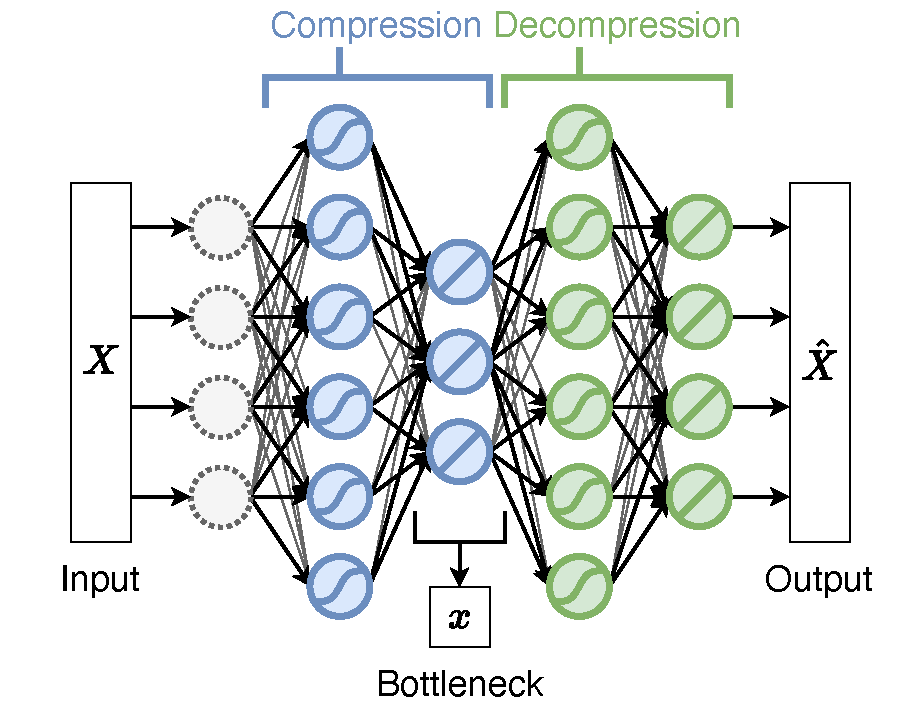
\includegraphics[width=0.84\textwidth]{background/figures/auto-associative.pdf}
    \caption[Overview of an Auto-Associative Network]{Overview of a non-linear Auto-Associative Network. For compression, which is coloured in blue, the input $X$ is first fed through a sigmoid-activated encoding layer and is then compressed to a lower-dimensional bottleneck representation $x$ using a linear activation. For decompression, which is coloured in green, the bottleneck representation $x$ is fed through a sigmoid-activated decoding layer and is then decompressed using a linear activation into $\hat{X}$, approximating $X$. The activation function used by each neuron is indicated symbolically. This schematic is inspired by Figure 1 in \textcite{auto-associative-2001}.}
    \label{fig:auto-associative-overview}
\end{figure}

\noindent In the fruit classification examples, an auto-associative network might learn that round fruit are green whilst crescent-shaped fruit are yellow, and thus encode each fruit only by its colour. During the decoding step, it would then use this learned assumption to reconstruct green fruit as round and yellow fruit as crescent-shaped. Given the limited training data in this example, such a simple auto-associative network would perform very well on ID data of green apples and yellow bananas. However, how would it deal with pictures of yellow apples and green bananas? The encoding step would function as usual and extract only the fruit's colour. However, during decoding, the network would reconstruct erroneously and translate the \textit{yellow} apple into a \textit{yellow} banana and the \textit{green} banana into a \textit{green} apple. The magnitude of such an auto-associative network's reconstruction error, which can be measured as the squared residuals between the input $X$ and the output prediction $\hat{X}$, can thus be used to differentiate between ID and OOD inputs.

\newpar How does one decide on the dimensionality of the bottleneck and the encoding and decoding layers? Setting either too small may cause the network to be unable to replicate the structural complexity within the data and thus force it to make a high-bias underfit. In contrast, making the hidden layers of the auto-associative network too big may allow the network to overfit by memorising some of the natural (random) variance in the data. Instead, \textcite{auto-associative-2001} suggest finetuning the dimensionality hyperparameters by minimising complexity-relative error metrics such as Akaike's Final Prediction Error FPE \cite{akaike-fpe-1969, akaike-fpe-1970, akaike-fpe-1971}, or Akaike's Information Criterion AIC \cite{akaike-aic-1974}, which \citeauthor{auto-associative-2001} specialise for auto-associative networks as:
\begin{equation*}
    FPE = \frac{E}{2N} \cdot \frac{1 + \frac{W}{N}}{1 - \frac{W}{N}}
\end{equation*}
\begin{equation*}
    AIC = \ln{\left(\frac{E}{2N}\right)} + 2 \cdot \frac{W}{N}
\end{equation*}
where $E$ is the auto-associative network's squared prediction error, $W$ is its number of trainable weights, and $N$ is the number of input values \cite{auto-associative-2001}.

\newpar As the auto-associative network learns to compress the input data into a lower-dimensional form, it transforms highly correlated features into a smaller set of independent features. Training a machine learning model on this compressed feature vector $x$ instead of the higher-dimensional input $X$ has two clear advantages. First, it reduces the computational burden of training and evaluating the prediction model. Second, it helps models, like linear regression, that struggle with collinear features \cite{regression-collinearity-1984}, i.e. input features that can be expressed as a linear combination of each other. Crucially, since the auto-associative network learns to exploit any correlations, i.e. structural relationships, in the ID training data that a machine learning model could turn into closed-world assumptions, e.g. $\text{round} \leftrightarrow \text{green}$ and $\text{crescent-shaped} \leftrightarrow \text{yellow}$, an unusually high reconstruction error in the network indicates that a prediction \textbf{cannot} be made since some of the closed-world assumptions are violated. In contrast, a low error indicates that the model was trained on data following the same structure, and thus a prediction can be made.

In summary, an auto-associative network identifies the ID input data's underlying structural relationships. It can thus serve as an indicator for when the closed-world assumption is broken and a model trained on the same ID data cannot be trusted to make a prediction. However, since the auto-associative network has no information about the output labels or a model's predictions, it cannot be used for uncertainty quantification.

\subsection{Calibrating Out-Of-Distribution Confidence Scores}

The previous sections have summarised several methods to detect novel inputs that deviate from ID training data. Most of these methods provide an indicator value and use a threshold to classify ID vs OOD inputs. How is that threshold set? How can the underlying indicator be translated into a calibrated confidence score?

\newpar \textcite{learning-ood-confidence-2018} use the concept of hints as a very intuitive approach to determine how confident a model is in that it can make a prediction. In a nutshell, if the model is unsure, it can ask for a hint for the correct prediction at a minor penalty. It is rewarded if it is correct without using hints, but if it is wrong without using hints, it is punished. When the model is later applied to unseen data and asks for a hint, the need for a hint can be seen as an indication that an input is OOD.

In particular, the authors propose to have the model output a confidence score $c \in [0; 1]$ alongside its prediction. This prediction, $m(X) = \hat{Y}$, is now conditioned on $c$, which we henceforth denote as $\hat{Y} \given c$. During training, the model's prediction $\hat{Y}$ is replaced by a new prediction $\hat{Y}'$ that is augmented with the target value $Y$ depending on $c$, i.e. $\hat{Y}' = c \cdot \hat{Y} + (1-c) \cdot Y$. Suppose the model has little confidence and wants a hint. In that case, it can output $c \rightarrow 0$, thus mostly replacing its prediction with the true target value and reducing the misprediction penalty it would otherwise receive. By itself, this hint-augmented prediction allows the model to always predict zero confidence without any penalty. Thus, the model's original loss function $\mathcal{L}_Y$, which penalises mispredictions between $\hat{Y}'$ and $Y$, is replaced by $\mathcal{L} = \mathcal{L}_Y + \lambda \cdot \mathcal{L}_c$ where $\mathcal{L}_{c} = - \log_{2}{c}$ penalises low confidence values. As a result, the model is incentivised to predict high confidence when it can make a good prediction since the misprediction penalty is low. When it cannot make a prediction, it is encouraged to predict low confidence instead. Here, $\lambda$ is a hyperparameter that controls the cost of hints. To ensure that the model does not only predict high confidence values as the predictor's accuracy improves during training, \citeauthor{learning-ood-confidence-2018} propose a simple scheme where $\lambda$ is adjusted continuously to keep $\mathcal{L}_c$ close to some budget $\beta$, e.g. $\beta = 0.3$. 

The confidence value $c$ is intuitively interpretable. However, augmenting the prediction based on $c$ during training also means that gradient propagation through the network is obstructed, especially for low-confidence predictions and at the beginning of training. To mitigate this issue, \citeauthor{learning-ood-confidence-2018} suggest only performing the conditioning on $c$ probabilistically, e.g. only for $50\%$ of the inputs in a training batch.

\newpar How can one differentiate between ID and OOD inputs with this confidence score? While finding a threshold that separates both cases is a proven solution, it does not by itself answer the initial question of how to select this threshold and how to ensure that the confidence value $c$ is meaningful even though only ID inputs are provided during training. \citeauthor{learning-ood-confidence-2018} propose using data augmentation to invent some difficult maybe-OOD inputs at training time so that the model can already be trained to have low confidence for those. In a classification task, some noise can be added to the inputs, either randomly or adversarially with the fast gradient sign method \cite{fast-gradient-2014}. If the model misclassifies them, it is forced to assign these maybe-OOD inputs a lower confidence score. Such misclassified samples can then be used to find the threshold between ID and OOD inputs such that correctly classified ID inputs are definitely recognised as ID and misclassified maybe-OOD inputs are designated as OOD.

\newpar \textcite{ood-exposure-confidence-2021} showcase a different method that uses outlier exposure \cite{ood-exposure-2018} to calibrate the softmax confidence scores (see \Cref{txt:softmax-confidence}) of a classification network. In particular, for OOD inputs, the softmax scores for all classes should approach the uniform distribution, i.e. show zero confidence. In contrast, the confidence score for ID inputs should resemble the classification accuracy and thus be interpretable, similar to \citeauthor{learning-ood-confidence-2018}'s hints. While prior work minimised the Kullback-Leibler (KL) divergence \cite{kl-divergence-1951} between the softmax and the uniform distribution for OOD inputs \cite{ood-exposure-2018}, \citeauthor{ood-exposure-confidence-2021} instead minimise the total variation distance, which results in more uniform OOD scores. Furthermore, they suggest pushing the ID confidence towards the network's average classification accuracy during training to achieve their second calibration goal. Since this intrusively changes the loss function, it requires retraining the classifier. The authors also highlight that outlier exposure can also be combined with post-hoc methods for OOD detection, including adversarial OOD detection (see \Cref{txt:ood-distance}) and Boundary Aware Learning and OOD sample generation (see \Cref{txt:ood-input-generation}).

\citeauthor{learning-ood-confidence-2018}'s work and \citeauthor{ood-exposure-confidence-2021}'s work both highlight the challenge of calibrating OOD input detectors. While clearly-OOD datasets are available in some domains, when they are lacking, a model should still be trained with some maybe-OOD inputs obtained through noise or adversarial generation to ensure that a close boundary between ID and OOD inputs is indeed learned.

\subsection{Synthesising OOD Samples for Training OOD Detectors} \label{txt:ood-input-generation}

OOD detection is used to filter out inputs that violate the closed-world assumption, as a machine learning model cannot make predictions for them. Some OOD inputs are simple to detect, such as showing an image of a purple fish to the fruit classification model. However, other inputs lie much closer to the manifold of ID examples and are thus much more difficult to detect. Adversarial Methods such as the fast gradient sign method \cite{fast-gradient-2014} are built to generate inputs that can fool a network into making the wrong prediction with only a small change in input. Thus, building an OOD detector that learns a close boundary around the ID data manifold and can detect OOD inputs that lie close to this boundary is worthwhile.

\newpar \textcite{ood-boundary-2021} propose the Boundary Aware Learning method, which trains an ID vs OOD discriminator using both trivial and increasingly hard synthetic examples of OOD inputs. This post-hoc method adds a Generative Adversarial Network to a pre-trained classification prediction network, which is briefly introduced in the following paragraph.

\newpar Generative Adversarial Networks (GANs) are generative models that learn the distribution of the training data and how to distinguish it from other inputs \cite{gan-2014}. They consist of two sub-models, a generator and a discriminator. While the generator is trained to generate samples that appear as if they have come from the training distribution, the detector is optimised to tell the generated samples apart from the true training inputs. Thus, they compete in a two-player minimax game. Specifically, the detector $D(x)$ and generator $G(z)$, where $z$ may be sampled from a multivariate normal distribution $\mathcal{N}$, is optimised to predict the probability that some input $x$ comes from the training data $X$ using the following two-player minimax game value function \cite{gan-2014}:
\begin{equation}
    \min_{G} \max_{D} V(G, D) = E_{x \in X}[\log D(x)] + E_{z \sim \mathcal{N}}[\log{(1 - D(G(z)))}]
\end{equation}

\newpar The GAN-based Boundary Aware Learning method is composed of three modules that split the responsibility for generating OOD samples:
\begin{enumerate}
    \item The \textbf{Representation Extraction Module} generates trivial OOD inputs that are used to roughly train the discriminator. Prior work often used normal distributions to generate such OOD samples in an upstream layer, e.g. \cite{distance-confidence-2017, ood-adversarial-detection-2018}. However, the authors note that the underlying assumption that features in an upstream layer follow a normal distribution is often wrong. Instead, they suggest sampling uniformly from the feature space, bounded by the minimum and maximum feature values within a training batch, and assigning random output classes to these inputs. The uniform sampling improves the OOD detection performance by ensuring that the often sparsely-in-distribution feature space is sampled diversely. However, some of these uniformly distributed inputs may, by chance, be close to some ID training samples. In that case, the true training class labels would conflict with the random OOD labels, thus confusing the discriminator into being less confident even when ID inputs are predicted correctly.
    \item The \textbf{Representation Discrimination Module} is trained to learn the boundary between ID and OOD samples using two additional loss function terms for the GAN's discriminator. First, the \textbf{Shuffle Loss} trains the discriminator to be unconfident for ID inputs with shuffled wrong class label outputs. Second, the \textbf{Uniform Loss} trains it to have high confidence for ID inputs and low confidence for trivial OOD inputs. Since some of the trivial OOD samples may overlap with ID samples, more emphasis is put on having high confidence in ID inputs. In contrast, hard OOD inputs, which the Representation Sampling Module generates, should not have conflicts and are thus used as OOD samples with high emphasis.
    \item The \textbf{Representation Sampling Module} generates increasingly hard OOD inputs at the boundary to the ID manifold, thus pushing the discriminator to learn a tighter separation boundary. It first samples synthetic ID inputs within the ID manifold using the GAN's generator. Next, the fast gradient sign method \cite{fast-gradient-2014} is used to push these inputs into more-OOD areas, i.e. towards the boundary. The FGSM's step magnitude is sampled from a normal distribution to train with diverse step lengths. Crucially, the synthetic ID generator is incentivised to generate inputs that are increasingly close to the ID training data, pushing the OOD samples closer to the ID boundary and making them increasingly hard to classify.
\end{enumerate}

\noindent In combination, these three components post-hoc train an ID vs OOD discriminator that learns the boundary of the ID manifold. The uniform sampling of trivial OOD inputs ensures that the vast majority of the input data space is correctly identified as OOD. Furthermore, synthetic ID inputs are transformed into hard OOD inputs using an adversarial gradient descent step to tighten the boundary. However, only relying on the gradual improvement of the synthetic ID generator is insufficient to bring the OOD samples as close to the ID manifold boundary as possible, i.e. without damaging the confidence for ID inputs.

\newpar \textcite{ood-training-2017} propose a method to generate even more challenging OOD input samples for training a classification network. They use a GAN whose generator is trained to learn the in-distribution manifold and produce ID samples to fool a discriminator that attempts to distinguish between real and synthetic ID samples. Additionally, the authors add a new term to the GAN's loss function that pushes the synthetic samples into low-density regions, i.e. where few ID training samples are and which can thus be classified as OOD regions. Overall, this forces the GAN to produce OOD samples that are at the boundary of the ID manifold, which is sufficient to teach an OOD detector about further-away OOD regions as well \cite{noise-contrastive-uq-2020}. \citeauthor{ood-training-2017} also augment their classification network with a confidence loss function that minimises the KL divergence between the uniform distribution and the softmax scores for OOD inputs, similar to the approach used in outlier exposure \cite{ood-exposure-2018}. This adjusted classification network and the OOD GAN can be trained separately or jointly. In the latter case, the KL divergence loss is shared between the GAN and classification network.

\subsection{Uncertainty-based Methods for Novelty Detection} \label{txt:uq-conf-method}

It may seem attractive to treat novelty detection and uncertainty quantification using the same approach. After all, while some (often adversarial) out-of-distribution inputs are outside the problem domain, many are semantically valid inputs that should have been sampled in a more comprehensive training data collection process. These latter inputs are thus only OOD as the result of incomplete knowledge about the input distribution, and they can be detected if high epistemic uncertainty is assigned to them. Existing (Bayesian) uncertainty quantification methods such as Monte Carlo Dropout \cite{mc-dropout-2016}, Batch Normalised Deep Networks \cite{batch-normalized-uq-2018}, Deep Ensembles \cite{deep-ensembles-2017}, and Gaussian Processes \cite{gp-ml-2005} can and have been applied to detect novel inputs as high-uncertainty inputs. For instance, \textcite{ensemble-uncertainty-ood-2021} show that their deep ensemble of neural networks using random initialisation, per-epoch shuffling, and dropout layers is able to detect OOD inputs. However, if a method is not explicitly trained with OOD inputs, it cannot guarantee that it predicts high uncertainty outside the ID manifold.

\newpar \textcite{noise-contrastive-uq-2020} present a probabilistic modelling approach combining uncertainty quantification and OOD detection. They utilise noise contrastive priors to teach the model to distinguish between the ID training data and inputs that have been perturbed with noise. Thus, the model learns that its inputs have a larger domain than just the ID examples. In particular, in addition to training the model to predict the target $Y$ for an input $X$, the authors also train it to recover a Gaussian-perturbed output $\text{N}(Y, \sigma_{Y}^{2})$ from a Gaussian-perturbed input $\text{N}(X, \sigma_{X}^{2})$ and thus ensure that the model must predict with higher uncertainty for the perturbed inputs. However, if this approach were broadly applied, some of the perturbed inputs might clash with ID inputs and thus confuse the network's training with their perturbed outputs. Instead, the authors only generate noise-perturbed inputs near the ID data boundary (see \Cref{txt:ood-input-generation}). They demonstrate that only encouraging the model to become more uncertain at the boundary also trains it to be uncertain for OOD inputs further away from the boundary.

The authors also investigate whether a model with noise contrastive priors can be used in active learning to select new training data points that would quickly improve the model's performance. Intuitively, such data points should be in areas of high uncertainty, i.e. either OOD inputs or ID inputs in areas where the output changes with high frequency. \citeauthor{noise-contrastive-uq-2020} find that the following acquisition rule based on the expected information gain performs well with their noise contrastive priors:
\begin{equation*}
    (x_\text{new}, y_\text{new}) \sim P_\text{new}(x_{new}, y_{new}) \propto \left( 1 + \frac{\text{Var}[q(\mu(x))]}{\sigma^2(x)} \right)^{\frac{1}{\tau}}
\end{equation*}
where $P_\text{new}(x_{new}, y_{new})$ is the selection probability for a new data point $(x_\text{new}, y_\text{new})$, $q(\mu(x))$ is the predicted epistemic uncertainty, $\sigma^2(x)$ is the expected aleatoric uncertainty, and $\tau = 0.5$ is the sampling temperature.

\newpar It is worth noting that this approach makes significant assumptions about the output domain of the modelled process. In particular, it assumes that OOD inputs map to outputs from the same range as already seen with ID inputs and that high uncertainty across the ID output range can thus be used to describe the uncertainty in the OOD output range. However, if the output domain does not have problem-domain-specific bounds, the outputs could be of any unknown range. If, for instance, a coverage-based uncertainty metric like the predicted standard deviation is used, it would then have to cover an unknowably broad range. In these cases, it is thus beneficial to split OOD detection from uncertainty quantification and condition both the predicted value and its predicted uncertainty on the un-novelty of the input -- ID value and uncertainty predictions can be trusted, but both value and uncertainty predictions for OOD inputs should be discarded.


    %% Motivation and description of Icarus RSM
    \chapter{Prudent Response Surface Models} \label{txt:icarus-chapter}

Machine Learning has rapidly increased in capability and popularity over the past decade \cite{ml-trends-2021, ml-applications-2021}. Today, deep neural networks trained on climate simulation data can produce high-quality predictions at a tiny fraction of the time and computational cost \cite{neural-architecture-search-2021}. In addition, reduced complexity Response Surface Models (RSMs) are adopting newer machine-learning methods \cite{deep-rsm-2020} and are increasingly pushing down the required amount of training data. {\fontfamily{lmss}\selectfont Thus, an idea arises:}

\columnratio{0.4}
\begin{paracol}{2}
    {\fontfamily{lmss}\selectfont
    \begin{center}
        \textit{What if we, too, could train a machine-learning response surface model for our complex process model?}

        \textit{What if it would only take seconds instead of hours to perform a model run?}

        \textit{What if we could use those fast evaluations to run complex Monte Carlo data analysis on our new results?}

        \textit{What if we could do so with even less training data to make retraining cheaper for our frequently evolving complex model?}
    \end{center}

    \noindent Using GPU acceleration, a deep neural network is quickly trained and even performs well on the held-out test dataset. To increase confidence in the results, we add an error bar by having a second network predict the errors of the first. Evaluating this new RSM is fast, and hooking up some data-hungry downstream analysis that consumes the normal distributed predictions is easy.

    \newpar Oh, how soaring our celebration of success! Just before applying the RSM to input data from around the world, we check the input feature distribution. One of the features was constant during training. Changing it to any other value has absolutely no impact on the error bar. Validating the RSM on more testing data reveals that the predicted error bars are in no relation to the growing prediction error. Our confidence sinks.
    }

    \switchcolumn

    \begin{figure}[H]
        \centering
        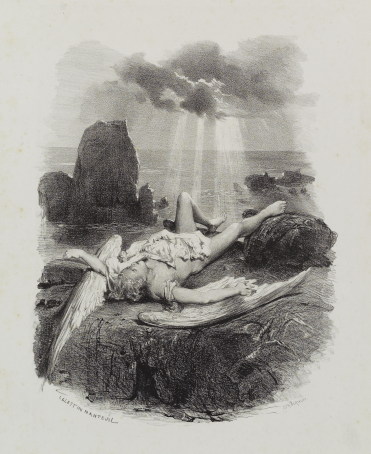
\includegraphics[width=0.55\textwidth]{icarus/figures/icarus.png}
        \caption[Icarus Fallen by C\'elestin Nanteuil]{Icarus Fallen (1845) by C\'elestin Nanteuil \cite{icarus-1845}. The New York Public Library. Available in the public domain.}
    \end{figure}
\end{paracol}

{\fontfamily{lmss}\selectfont
\newpar \textit{What if the seemingly simple downstream data analysis performed on the RSM's predictions also queried the RSM on similarly novel inputs? What if the RSM made gross mispredictions for those inputs, too, without any warning that it had been driven beyond its limits? How could we trust the final results of this analysis?}

\newpar Freefall. Daedalus weeps.
}

\section{The Virtue of Prudence} \label{txt:prudent-rsm}

Performing scientific analysis depends on knowing the uncertainty around a measurement or simulation result and assigning varying levels of confidence to a conclusion. As the quality of machine learning methods increases, it may be tempting to use a well-performing model and take its predictions at face value. However, prediction models make mistakes. \Cref{txt:uncertainty-quantification} has reviewed several methods that can be used to estimate the error that a prediction model might make, i.e. to quantify its uncertainty. However, models can also be fed with out-of-distribution inputs that differ vastly in their structure from what the model was trained on, which \Cref{txt:novelty-detection} has discussed. For example, suppose a model trained to predict a cat's age is presented with a picture of the Andromeda galaxy. In that case, neither the predicted age nor the estimated uncertainty likely makes much sense. Therefore, a machine-learning model should be \textit{prudent} in such cases.

\newpar We define being \textbf{prudent} as ``showing good judgment in avoiding risks and uncertainties'' \cite{prudent-dictionary-2023}, following the Cambridge Academic Content Dictionary. In the context of machine-learning-based response surface models (RSMs), a prudent RSM should:
\begin{enumerate}
    \item communicate how \textbf{confident} the RSM is that it can make a prediction at all
    \item communicate the level of \textbf{uncertainty} in its prediction
    \item exercise \textbf{prudence} by avoiding overconfident predictions
\end{enumerate}
\noindent In this chapter, we present the Icarus architecture for prudent RSMs (\Cref{txt:icarus-rsm}) and highlight how its predictions, uncertainty, and confidence can be utilised (\Cref{txt:icarus-propagation}). The components of this architecture are explored individually in \Cref{txt:ood-detection-chapter}, \Cref{txt:prediction-chapter}, and \Cref{txt:uncertainty-chapter} using a new dataset introduced in \Cref{txt:sosaa-data-chapter}. In \Cref{txt:icarus-evaluation-chapter}, we put Icarus to the test and build and evaluate an RSM for the SOSAA model (see \Cref{txt:sosaa-model}). Finally, \Cref{txt:icarus-preview} closes with some conclusions and a more detailed preview of the following chapters.

\section{Icarus: An Architecture for Prudent Response Surface Models} \label{txt:icarus-rsm}

The \textbf{Icarus} architecture combines three modules to construct \textit{prudent} response surface models (RSMs, see \Cref{txt:response-surface-models}). The architecture does not specify how these modules should be implemented but provides a blueprint for combining them. The most well-known component of Icarus is its \textcolor{icarus-prediction}{\textbf{prediction model}}, which is tasked with predicting the target variable $Y$ for new inputs $X$ to approximate the response surface of the underlying process that the RSM is being fitted to. The prediction model is trained with pairs of inputs $x \in X_{\text{train}}$ and their corresponding outputs $y$. These input-output pairs come from a set of training data, which represents the in-distribution. It is important to note that existing response surface models have primarily performed only this prediction task and can be used as a prediction model inside Icarus. In other words, an existing RSM can be wrapped with the Icarus architecture to extend its functionality and make it prudent.

The prediction model only produces point-predictions \textcolor{icarus-prediction}{$\hat{Y}$}. However, the prediction target variable $Y$ may have intrinsic aleatoric uncertainty, meaning some inputs may not correspond to just one true value but rather a distribution of values. Furthermore, the prediction model is generally imperfect and may thus predict values that are close but not equivalent to any true value. Therefore, the second component of Icarus is an \textcolor{icarus-uncertainty}{\textbf{uncertainty quantifier}} that is tasked with quantifying the prediction uncertainty of the prediction model. Given the input $X$ and point-prediction \textcolor{icarus-prediction}{$\hat{Y}$}, it estimates the distribution of true values $Y$ around the prediction \textcolor{icarus-prediction}{$\hat{Y}$}, which allows separating aleatoric uncertainty in the data from epistemic uncertainty in the prediction model (see \Cref{txt:aleatoic-epistemic-uncertainty}). We denote this uncertainty distribution with \textcolor{icarus-uncertainty}{$\hat{\Sigma}$}. Since prediction models usually perform worse outside their training data, the uncertainty quantifier should be trained and calibrated on a validation data set that is disjoint from the predictor training data but also comes from the in-distribution.

It is worth remembering that both the prediction model and uncertainty quantifier are only trained on in-distribution training data and can thus only perform their tasks on unseen inputs that are also in-distribution. To avoid trusting their predictions for out-of-distribution (OOD) inputs, the third and most crucial component of the Icarus architecture is an \textcolor{icarus-confidence}{\textbf{out-of-distribution detector}}. Given an unseen input $x \in X$, it is tasked with identifying whether $x$ is in-distribution, i.e. comes from the same distribution as the training data. The OOD detector produces a confidence score \textcolor{icarus-confidence}{$c$} between zero and one that represents the probability that the input comes from the in-distribution and that the prediction model and uncertainty quantifier can produce valid estimates. In the most general case, only the in-distribution (ID) training dataset is available and has to suffice for training the OOD detector. However, by identifying an existing dataset as out-of-distribution or synthesising OOD inputs, the OOD detector can also be trained and calibrated with both ID and OOD inputs.

\begin{figure}[H]
    \centering
    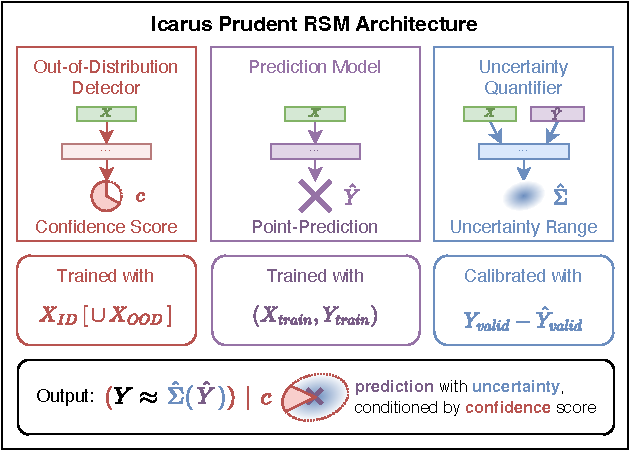
\includegraphics[width=0.915\textwidth]{icarus/figures/icarus-rsm.pdf}
    \caption[Overview of the prudent Icarus RSM Architecture]{Overview of the prudent Icarus RSM Architecture, which consists of three components. The out-of-distribution detector predicts a confidence score \textcolor{icarus-confidence}{$c$}, the prediction model estimates the target variable $Y$ with a point-prediction \textcolor{icarus-prediction}{$\hat{Y}$}, and the uncertainty quantifier predicts and calibrates the prediction uncertainty distribution \textcolor{icarus-uncertainty}{$\hat{\Sigma}$}. Inspired by \textcite{learning-ood-confidence-2018}, the uncertain output prediction is conditioned on the confidence score.}
    \label{fig:icarus-rsm}
\end{figure}

\noindent \Cref{fig:icarus-rsm} provides an overview of the architecture of the Icarus RSM and its three components described above. Crucially, the Icarus RSM does not only report a point-prediction \textcolor{icarus-prediction}{$\hat{Y}$}, but outputs a prediction with its uncertainty \textcolor{icarus-uncertainty}{$\hat{\Sigma}$}. Moreover, both the prediction and the uncertainty are conditioned on an additional output, the confidence score \textcolor{icarus-confidence}{$c$}. Thus, the output of an RSM following the Icarus architecture can be interpreted as follows:

\newpar For any input in $X$, the RSM predicts an output $\textcolor{icarus-confidence}{(}Y \sim \textcolor{icarus-uncertainty}{\hat{\Sigma}(}\textcolor{icarus-prediction}{\hat{Y}}\textcolor{icarus-uncertainty}{)}\textcolor{icarus-confidence}{) \given c}$. For the given confidence level \textcolor{icarus-confidence}{$c$}, the input is out-of-distribution with probability $1-\textcolor{icarus-confidence}{c}$, and the RSM's prediction $\textcolor{icarus-uncertainty}{\hat{\Sigma}(}\textcolor{icarus-prediction}{\hat{Y}}\textcolor{icarus-uncertainty}{)}$ must be ignored. With probability \textcolor{icarus-confidence}{$c$}, the input is in-distribution, and a valid prediction has been made. In this case, the RSM predicts that the true output $Y$ is drawn from the distribution $\textcolor{icarus-uncertainty}{\hat{\Sigma}(}\textcolor{icarus-prediction}{\hat{Y}}\textcolor{icarus-uncertainty}{)}$, which describes the uncertainty in the point-prediction \textcolor{icarus-prediction}{$\hat{Y}$}. While the uncertainty distribution is typically assumed to be normal, i.e. $Y \sim \text{N}(\textcolor{icarus-prediction}{\hat{Y}}, \textcolor{icarus-uncertainty}{\sigma^2(}\textcolor{icarus-prediction}{\hat{Y}}\textcolor{icarus-uncertainty}{)})$ or more concisely $Y \approx \textcolor{icarus-prediction}{\hat{Y}} \textcolor{icarus-uncertainty}{\pm \sigma}$, the more general notation of $Y \sim \textcolor{icarus-uncertainty}{\hat{\Sigma}(}\textcolor{icarus-prediction}{\hat{Y}}\textcolor{icarus-uncertainty}{)}$ also allows for non-normal uncertainty distributions.

\section{Propagating Confidence and Uncertainty} \label{txt:icarus-propagation}

A response surface model built with the Icarus architecture predicts confidence and uncertainty alongside the target value prediction. With the interpretation given above, RSM predictions on out-of-distribution inputs, inputs with high aleatoric or epistemic uncertainty, and inputs with an accurately predicted single true value can all be used and analysed together. If we want to perform some downstream analysis on these predictions, it is crucial to propagate both confidence and uncertainty through all analyses to the final result. In this section, we briefly outline several possible approaches for this propagation.

\newpar Monte Carlo analysis provides an intuitive, easy-to-implement approach for propagating confidence and uncertainty. Here, each prediction is interpreted as a random variable:
\begin{equation*}
    \textcolor{icarus-confidence}{(}Y \sim \textcolor{icarus-uncertainty}{\hat{\Sigma}(}\textcolor{icarus-prediction}{\hat{Y}}\textcolor{icarus-uncertainty}{)}\textcolor{icarus-confidence}{) \given c} = \begin{cases}
        \textcolor{icarus-confidence}{\text{OOD}} &\quad \text{with probability } 1-\textcolor{icarus-confidence}{c} \\
        Y \sim \textcolor{icarus-uncertainty}{\hat{\Sigma}(}\textcolor{icarus-prediction}{\hat{Y}}\textcolor{icarus-uncertainty}{)} &\quad \text{otherwise}
    \end{cases}
\end{equation*}
where the uncertainty distribution $\textcolor{icarus-uncertainty}{\hat{\Sigma}(}\textcolor{icarus-prediction}{\hat{Y}}\textcolor{icarus-uncertainty}{)}$ is sampled with probability \textcolor{icarus-confidence}{$c$}. Otherwise, the result is an \textcolor{icarus-confidence}{OOD} sentinel value that poisons the calculation, similar to \texttt{None}, \texttt{null}, or \texttt{NaN} values that cannot be used in further calculations. All prediction random-variables are sampled repeatedly, and the analysis is performed for each such sample. Clearly, analysis cannot be performed on poisonous OOD sentinel values. Therefore, the analysis is only performed on the ID samples, and the fraction of successful analyses is carried through as the confidence value of the analysis result. Finally, the distribution of all analysis results can be interpreted again as having a confidence value and an uncertainty distribution around a point-prediction value, e.g. the mean of the distribution.

\newpar The propagation of confidence can be seen as a monadic computation. For analyses that combine data points independently, e.g. when calculating the mean squared error over several predictions, the average confidence is propagated to the output. For analyses that analyse pairs of data points, the product confidence $\textcolor{icarus-confidence}{c_1} \cdot \textcolor{icarus-confidence}{c_2}$ is propagated. Both of these cases are intuitively handled with Monte Carlo analysis but can also be calculated analytically. Is this also possible for uncertainty propagation?

\textcite{correlated-propagation-2016} has introduced the \texttt{Measurements.jl} Julia package that uses linear error propagation theory to propagate the uncertainties of independent normally distributed measurements through analysis code in Julia. Specifically, a measurement variable \texttt{x} can be constructed as a mean value and standard deviation using the intuitive \texttt{x = 8.4 $\pm$ 0.7} syntax. Since the measurement type is a subtype of Julia's \texttt{AbstractFloat} abstract type, it can be used directly inside most numerical calculations and algorithms. For instance, \texttt{x+2} evaluates to \texttt{10.4 $\pm$ 0.4} and \texttt{2x} to \texttt{16.8 $\pm$ 1.4}. To handle the creation of correlated uncertainties, e.g. \texttt{x - x}, the measurement type internally keeps track of all independent measurements it is made up of, together with their associated uncertainties, an idea borrowed from the \texttt{uncertainties} Python package with similar functionality \cite{uncertainties-python-2022}. What if the input measurements have non-normally distributed uncertainties or are correlated? \textcite{srsm-phd-1999} presented methods to decompose uncertainties into independent (standard) normal random variables in their work on Stochastic RSMs (see \Cref{txt:stochastic-rsm}), which can be applied here as well. Uncertainties can be handled analytically without manual computation from the user using these approaches.

However, using subclassing and operator overloading can come with extraneous runtime overhead, especially for dynamically tracking all correlations, even though not all may be needed for the final result. As \textcite{autodiff-applications-2021} notes, auto-differentiation (see \Cref{txt:auto-differentiation}) can be generalised beyond automatically generating the code for derivative calculations to also be applied to automatically propagate uncertainties. While subclassing is one possible implementation of auto-differentiation, tools such as Tapenade \cite{tapenade-autodiff-2013} can be applied directly to source code and transform it to compute the derivatives alongside the values. A similar approach could be taken to automatically transform existing analysis algorithms implementations into ones that can propagate uncertainties and confidence. However, it is worth noting that while source code transformation tools work well for continuing to use existing code, encoding such capabilities in the type system, allowing some dependency tracking to be performed at compile time, and using an optimising compiler's capabilities to eliminate extraneous computations are more sustainable practices to supporting these computations.

\section{Summary of Prudent Response Surface Models} \label{txt:icarus-preview}

In this chapter, we have introduced the notion of \textit{prudent} response surface models (RSMs), which explicitly communicate their confidence about a prediction and its uncertainty (see \Cref{txt:prudent-rsm}). Importantly, prudent RSMs predict meaningful confidence scores and uncertainty distributions that are intuitive to interpret and can be integrated into downstream analysis. In \Cref{txt:icarus-rsm}, we presented Icarus, an architecture for constructing prudent RSMs. Icarus combines existing methods from out-of-distribution detection, uncertainty quantification and response surface modelling into one modular architecture. Since traditional RSMs fulfil one of these tasks, Icarus can be wrapped around existing RSMs, thus presenting a post-hoc improvement. Last but not least, we have briefly described how the confidence and uncertainty predicted by Icarus can be propagated from the RSM predictions through downstream analysis into the confidence and uncertainty of analysis results.

\newpar The remainder of this thesis is focused on exploring the Icarus architecture in more detail. \Cref{txt:ood-detection-chapter}, \Cref{txt:prediction-chapter}, and \Cref{txt:uncertainty-chapter} delve into the three Icarus components, out-of-distribution (OOD) detection, prediction, and uncertainty quantification. They investigate different implementations for each component and explore how they can be compared. While the OOD detector is primarily analysed using toy examples, the other two components are evaluated on a new dataset for the SOSAA model that is introduced in \Cref{txt:sosaa-data-chapter}. After these per-module explorations, we use our findings to build a baseline RSM for the SOSAA model using the Icarus architecture and evaluate its performance in \Cref{txt:icarus-evaluation-chapter}. Overall, we thus aim to give both more detailed, generally applicable insights into each part of Icarus, \textit{and} test it on a real-world example to enable future research to use and improve upon our method.


    %% SOSAA Dataset description and brief exploration
    \chapter{The SOSAA Trajectories Dataset} \label{txt:sosaa-data-chapter}

The SOSAA model is a chemistry transport model that has been actively developed in the Multi-Scale Modelling Group at the University of Helsinki since 2011 \cite{sosa-description-2011}. SOSAA was initially developed to run in stationary mode, in which it simulates the atmospheric processes near a measurement station. However, recent developments have focused on implementing a Lagrangian trajectory mode, in which emissions are picked up along the current mean meteorological trajectory that arrives at the station several days later. Please refer back to \Cref{txt:sosaa-model} for more detail on the SOSAA model and its components.

This project explores the feasibility of training a prudent Response Surface Model on SOSAA model runs using the Icarus architecture (see \Cref{txt:icarus-rsm}). We focus on the data from trajectory simulations since they provide SOSAA with external input about the emissions and meteorological conditions at every time step.

\newpar This chapter introduces the SOSAA trajectories dataset, which is published on \href{https://github.com/juntyr/sosaa-trajectories-dataset}{GitHub}. All runs in this dataset were performed with \href{https://version.helsinki.fi/putian.zhou/sosaa/-/tree/10618aa98c7470546308adf132afb0bc0735b4eb}{SOSAA@10618aa}. First, \Cref{txt:data-layout-variables} summarises the layout and variables of the dataset. Next, \Cref{txt:six-trajectories} explores the six trajectories that are included. Following on, \Cref{txt:space-time-expansion} introduces the space-time expansion procedure that is applied to all input variables, while \Cref{txt:ccn-target} details how the CCN concentration, which is used as a target variable in our experiments, is extracted from the data. Finally, \Cref{txt:feature-importance} analyses which features are most important to two simple machine learning prediction models.

\section{Description of the Dataset Layout and Variables} \label{txt:data-layout-variables}

The dataset is split into an extensive folder structure that contains the SOSAA configuration files (see \Cref{app:sosaa-settings} for an example) and the input and output NetCDF files \cite{netcdf-1989} for each of the trajectories. Each trajectory is identified by the time at which it arrives at the SMEAR II measurement station at Hyyti\"al\"a, Finland \cite{smear-station-2013}. Both the top-level \texttt{inputs/} and \texttt{outputs/} folders are split into \texttt{baseline/} and \texttt{perturbation/} directories. The former contains the baseline SOSAA runs that are used in this chapter. The \texttt{perturbation/} directory is further split by perturbation group and kind, which are explained in \Cref{txt:perturbation-generalisation}. These input directories are then split into \texttt{HYDE\_BASE\_Y2018/OUTPUT\_bwd\_\textcolor{purple}{YYYYMMDD}} folders based on the arrival date of the trajectories. Each of these folders contains an \texttt{EMISSIONS\_0422/} and a \texttt{METEO/} directory. For example, a trajectory that arrives on \textcolor{purple}{21.05.2018} at \textcolor{purple}{14:00 UTC} has the following four input files:
\begin{enumerate}
    \item aerosol emissions input: \texttt{EMISSIONS\_0422/\textcolor{purple}{20180521}\_7daybwd\_Hyde\_traj\_\textcolor{purple}{AER}\_\textcolor{purple}{10}\_L3.nc}
    \item anthropogenic emissions input: \texttt{EMISSIONS\_0422/\textcolor{purple}{20180521}\_7daybwd\_Hyde\_traj\_\textcolor{purple}{ANT}\_\textcolor{purple}{10}\_L3.nc}
    \item biogenic emissions input: \texttt{EMISSIONS\_0422/\textcolor{purple}{20180521}\_7daybwd\_Hyde\_traj\_\textcolor{purple}{BIO}\_\textcolor{purple}{10}\_L3.nc}
    \item meteorological conditions input: \texttt{METEO/METEO\_\textcolor{purple}{20180521}\_R\textcolor{purple}{10}.nc}
\end{enumerate}
Note that instead of the arrival hour \textcolor{purple}{14}, the input file names use the number of hours until midnight, \textcolor{purple}{10} in this case. In contrast to the input directories, the output folders are directly split by the full arrival time and use the natural time format instead:
\begin{enumerate}
    \setcounter{enumi}{5}
    \item SOSAA output: \texttt{\textcolor{purple}{20180521}\_T\textcolor{purple}{14}/output.nc}
\end{enumerate}
Each input and output file stores variables that are indexed by time first and often by height layer second. Since SOSAA can use arbitrary time and height resolution, these variables are linearly interpolated, which we mirror when loading these files. Biogenic emissions are a special case since they are only distributed amongst the layers reaching up to ten metres above the ground. Note that not all input variables are actually read in by the SOSAA model. For instance, only the air temperature \texttt{t}, specific humidity \texttt{q}, surface net solar radiation \texttt{ssr}, land-sea mask \texttt{lsm}, and atmospheric boundary layer height \texttt{blh} are used from amongst the meteorological variables. Thus, a model should also not be trained on them. We further exclude the layer pressure \texttt{lp} since it encourages easy overfitting on the layer height. Please refer to \Cref{app:sosaa-variables} for a complete list of the used input variables, and to \Cref{txt:ccn-target} for an explanation of how the CCN target variable is extracted from the output files. Note that both the inputs and outputs are standardised (see \Cref{txt:data-preprocessing}) based on their training data set before being used in any model.

\section{Six Representative Trajectories} \label{txt:six-trajectories}

At the start of this research project, access was provided to the inputs and outputs of 480 SOSAA trajectory runs. These 480 trajectories cover the time period from 09.05.2018 at 00:00 UTC until 28.05.2018 at 23:00 UTC, with one trajectory arriving at every full hour. In order to streamline the development and analysis of the Icarus-RSM for these trajectory datasets, we chose to focus on six example trajectories that cover different scenarios. The baseline and perturbation runs of these six trajectories and their temporal neighbours were then performed on the CSC Puhti supercomputer. The dataset of these six trajectories forms the baseline for all evaluations in \Cref{txt:icarus-evaluation-chapter} since they provide a quick overview of how a machine-learning model generalises beyond its training data across time and to unseen input scenarios.

\Cref{fig:six-trajectories-maps} shows the paths that each of the six trajectories takes over the $\geq 5$ days before it arrives at Hyyti\"al\"a. While SOSAA simulates $\geq 7$ days of the trajectory, the initial 48-hour warm-up period is excluded from the analysis. The main trajectory has a black outline and is coloured from white at the start over blue and purple to red at the time of arrival in Hyyti\"al\"a. In addition to this main trajectory, six temporally adjacent trajectories are plotted with thinner lines. Specifically, for a trajectory at time $t$, the trajectories at times $t-4\text{h}$, $t-2\text{h}$, $t-1\text{h}$, $t+1\text{h}$, $t+2\text{h}$, and $t+4\text{h}$ are plotted in blue, purple, orange, and yellow. All temporally adjacent paths should roughly line if the meteorological conditions are stable. In contrast, the trajectory that arrived in Hyyti\"al\"a on 23.05.2018 at 13:00 UTC rapidly evolved over the next four hours.

\newpar \Cref{app:six-trajectories} visually explores the input variables passed to the SOSAA model, including aerosol, anthropogenic and biogenic emissions and meteorological conditions. These inputs are summarised here alongside a description of the path that each of the six trajectories takes:
\begin{enumerate}
    \item The first trajectory starts in Sweden and travels clockwise over Russia and the Gulf of Finland before arriving in Hyyti\"al\"a on \textbf{14.05.2018} at \textbf{10:00} UTC. In this trajectory, most aerosol and anthropogenic emissions come from the time over Russia right before entering the Baltic Sea. Moreover, the temperature gradually increases until the arrival (see \Cref{fig:trajectory-inputs-14-05}).
    \item The second trajectory starts in Russia and travels counter-clockwise over the Baltics, then across to Sweden, and finally across the Gulf of Bothnia to Finland, where it arrives on \textbf{15.05.2018} at \textbf{19:00} UTC. Again, most aerosol and anthropogenic emissions originate in Russia and the Baltics (see \Cref{fig:trajectory-inputs-15-05}). While the temperature increase is less evident than the day before, the highest temperatures of up to $25 \degree \text{C}$ are limited to the final passage over Finland.
    \item The third trajectory starts in Estonia and travels clockwise across the Gulf of Finland to the west of Finland before turning towards Russia, from where it heads to its arrival at Hyyti\"al\"a on \textbf{17.05.2018} at \textbf{00:00} UTC. In this trajectory, most aerosol emissions come from the Baltics and eastern Finland (see \Cref{fig:trajectory-inputs-17-05}). Again, there is no clear temperature gradient.
    \item The fourth trajectory originates in eastern Canada, from where it crosses the Atlantic, over the southern coast of Iceland, before arriving in Norway, from where its path leads north-eastwards across Sweden and the Gulf of Bothnia to Finland, where it arrives on \textbf{19.05.2018} at \textbf{04:00} UTC. In this trajectory, most biogenic emissions come from the passage through the Nordic countries and, to a lesser extent, from Canada, with similar patterns for aerosol and anthropogenic emissions. While there is no clear pattern for the sub-zero-degree temperatures, there is a noticeable increase in above-freezing air temperatures towards the end of the trajectory (see \Cref{fig:trajectory-inputs-19-05}).
    \item The fifth trajectory starts north of Scotland, from where it travels eastwards to Norway. From Norway, it follows a clockwise bow-shape over southern Sweden and Denmark, before travelling north-eastwards towards Hyyti\"al\"a, where it arrives on \textbf{21.05.2018} at \textbf{15:00} UTC. All emissions are increased during this trajectory, with most aerosol and anthropogenic emissions occurring over Sweden. $\text{SO}_2$ emissions stand out as they are highest over Denmark and southern Norway (see \Cref{fig:trajectory-inputs-21-05}). Again, there is a clear temperature increase during the approach to Finland across the Gulf of Bothnia.
    \item The sixth and final trajectory starts north-west of Scotland from where it first travels southward over England, then sharply turns and travels northwards along the Norwegian coast before making yet another sharp turn to cross the Gulf of Bothnia from northern Sweden to southern Finland, where it arrives on \textbf{23.05.2018} at \textbf{13:00} UTC. In this trajectory, most aerosol and anthropogenic emissions originate over Scotland and England, while most biogenic emissions come from northern Sweden and Finland (see \Cref{fig:trajectory-inputs-23-05}). The sixth trajectory only shows a slight downward temperature gradient. It is worth noting that this trajectory is the least stable and rapidly transforms into an Atlantic-crossing path (similar to the 19.05. trajectory) over the next four hours.
\end{enumerate}

\begin{figure}[H]
    \centering
    \begin{subfigure}
        \centering
        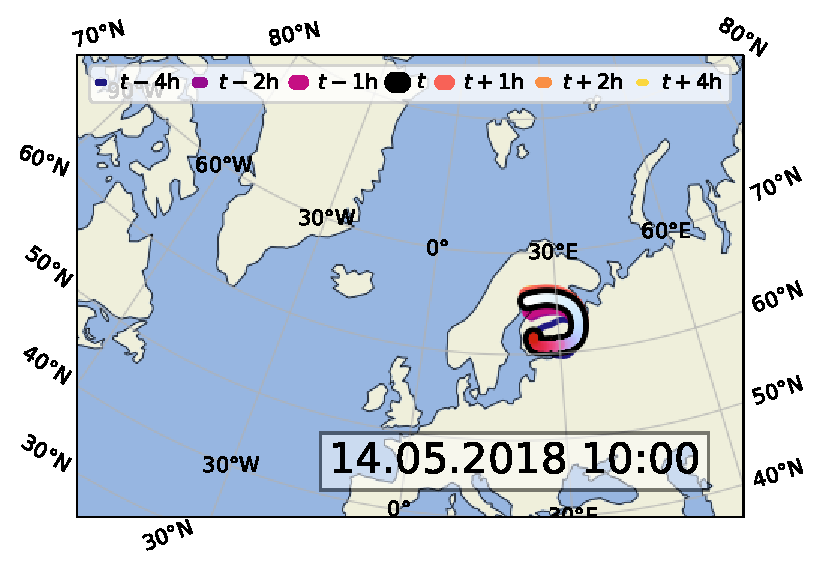
\includegraphics[width=0.49\textwidth]{sosaa-data/figures/trajectories/trajectory-14.05.2018:10.00.pdf}
    \end{subfigure}
    \begin{subfigure}
        \centering
        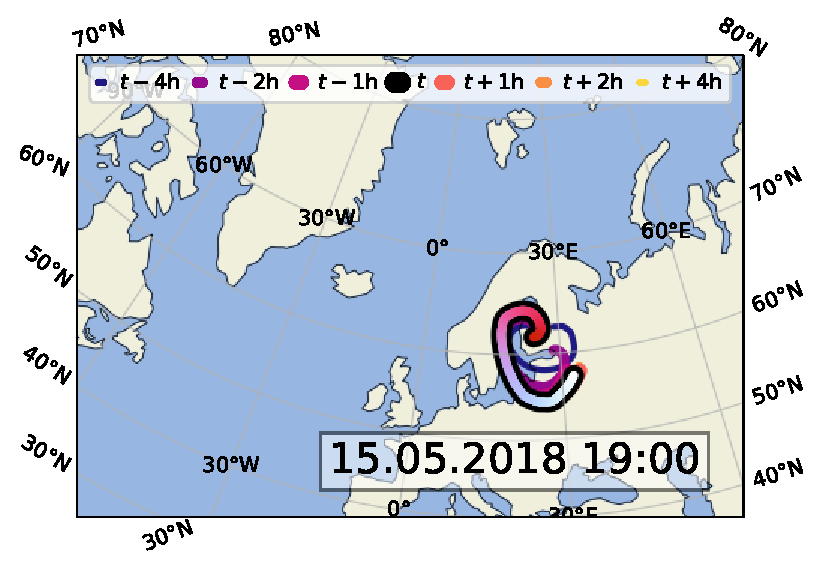
\includegraphics[width=0.49\textwidth]{sosaa-data/figures/trajectories/trajectory-15.05.2018:19.00.pdf}
    \end{subfigure}

    \begin{subfigure}
        \centering
        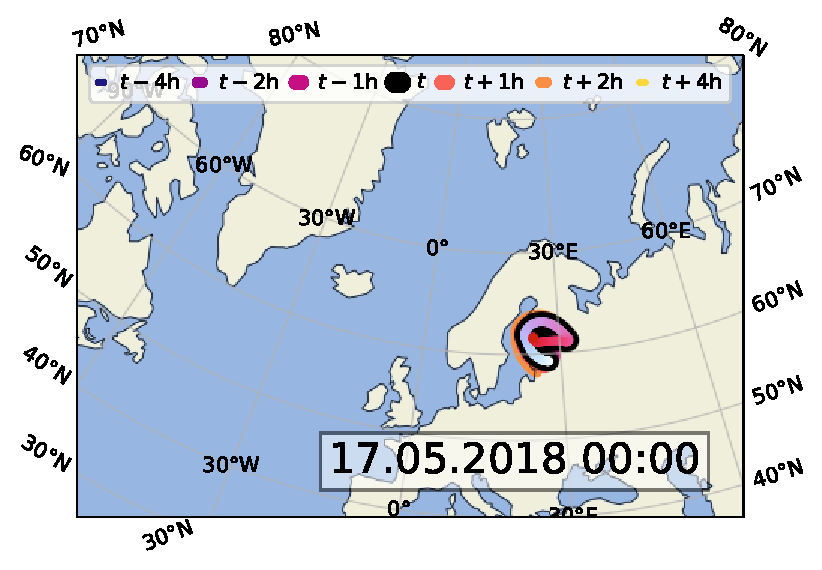
\includegraphics[width=0.49\textwidth]{sosaa-data/figures/trajectories/trajectory-17.05.2018:00.00.pdf}
    \end{subfigure}
    \begin{subfigure}
        \centering
        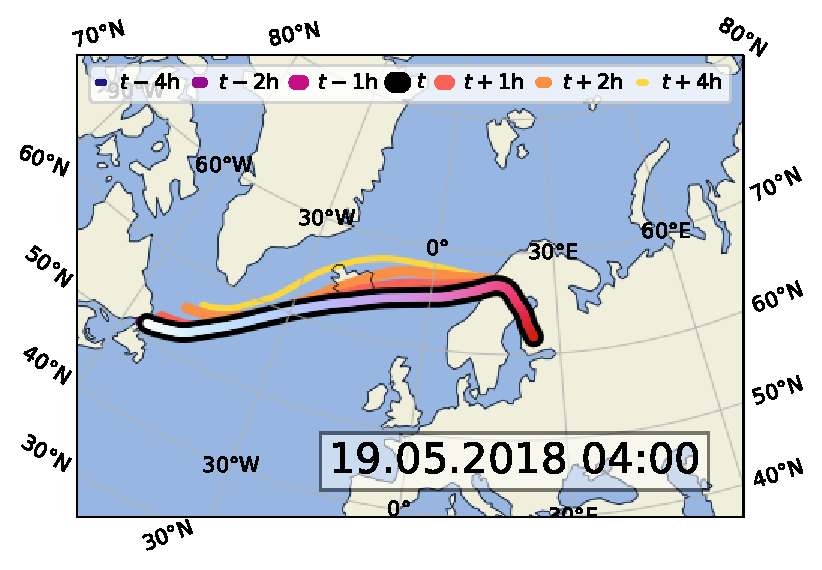
\includegraphics[width=0.49\textwidth]{sosaa-data/figures/trajectories/trajectory-19.05.2018:04.00.pdf}
    \end{subfigure}

    \begin{subfigure}
        \centering
        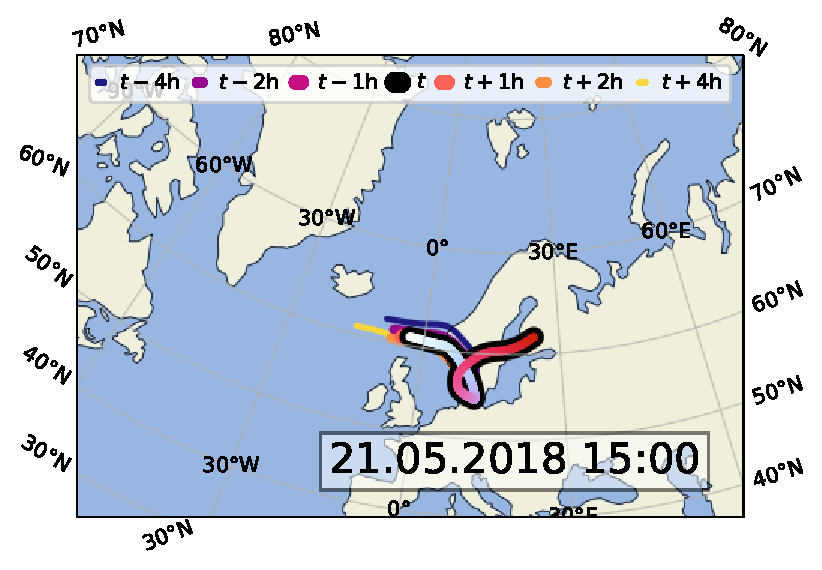
\includegraphics[width=0.49\textwidth]{sosaa-data/figures/trajectories/trajectory-21.05.2018:15.00.pdf}
    \end{subfigure}
    \begin{subfigure}
        \centering
        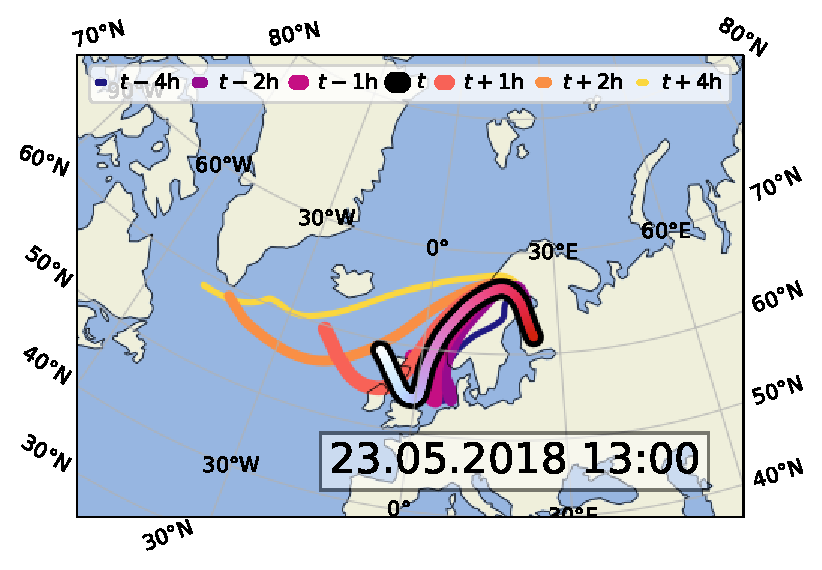
\includegraphics[width=0.49\textwidth]{sosaa-data/figures/trajectories/trajectory-23.05.2018:13.00.pdf}
    \end{subfigure}

    \caption[Maps for the six example trajectories]{Maps for the six example trajectories. Each map shows the time-coloured (see \Cref{fig:six-trajectories-ccn}) path of the trajectory that arrives at the listed time in Hyyti\"al\"a, as well as the paths of the prior and next trajectories.}
    \label{fig:six-trajectories-maps}
\end{figure}

\section{The Space-Time Expansion of Input Variables} \label{txt:space-time-expansion}

\begin{multicols}{2}
    \noindent When the SOSAA model runs in trajectory mode, it receives the current meteorological condition and emission input for every time step. In addition to these external inputs, SOSAA also carries over the internal state of every box from the previous time step. This internal state contains over two million variables across all height boxes. How can we train a Response Surface Model that independently predicts the CCN concentration for each box but also learns about the cross-box interactions? One idea is to train the RSM on the combination of the SOSAA inputs and the internal states of the previous time step. This method has the exciting extension of predicting not just the next CCN concentration but the entire state vector, allowing the emulation of the entire SOSAA model simply by stacking RSMs and running them across several time steps. While this approach would intuitively support long-term non-linear effects and produce exploding prediction uncertainty for multi-time step predictions, it would also complicate sensitivity analysis. If the CCN concentration is most sensitive to some variables of the prior state, the sensitivity would need to be evaluated recursively over several time steps and across several boxes to trace them back to the emissions. Instead, in this project, the Icarus-RSM is only trained on SOSAA's external inputs.

    \newpar How can long-term non-linear effects be captured if the RSM only receives the external inputs but cannot keep any state across time steps?

    \begin{figure}[H]
        \centering
        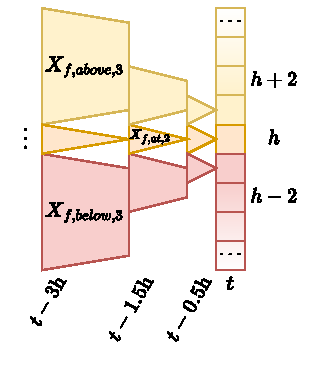
\includegraphics[width=0.49\textwidth]{sosaa-data/figures/space-time-expansion.pdf}
        \vspace{-3em}
        \caption[Input Feature Space-Time-Expansion]{Overview of the simultaneous space-time expansion of each feature $X_f(t, h)$ into $X_{f,s,i}(t, h)$. With seven time groups and an $above$, $at$, and $below$-height group, each feature is thus expanded into 21 space-time groups that summarise the influences from neighbouring SOSAA boxes.}
        \label{fig:space-time-expansion}
    \end{figure}
\end{multicols}

\noindent If the model receives the inputs not just from the current timestep and height level but from a larger range of prior time steps and surrounding boxes, it should again be able to capture these long-term effects. Therefore, we propose the following space-time expansion of the SOSAA input feature vector for the Icarus-RSM:

\begin{enumerate}
    \item \textbf{Time Expansion:} Each input feature $X_f(t)$ at time $t$ is expanded into the following seven temporally-averaged features:
    \begin{equation*}
        X_{f,i}(t) = \text{E}[\{ X_{f}(t') \given t + \Delta t_{lower, i} \leq t' \leq t + \Delta t_{upper, i} \}]
    \end{equation*}
    where $i \in 1..7$, $t_{lower} = \{ -0.5\text{h}, -1.5\text{h}, -3\text{h}, -6\text{h}, -12\text{h}, -24\text{h}, -48\text{h} \}$ and $t_{upper} = \{ -0.5\text{h}, -1\text{h}, -2\text{h},$ $-3.5\text{h}, -6.5\text{h}, -12.5\text{h}, -24.5\text{h} \}$. Note that SOSAA was configured to output predictions every $30 \text{min}$ for the trajectories dataset, which explains the half-hour time intervals.

    \item \textbf{Space Expansion:} Each input feature $X_f(h)$, where $h$ is the box height layer index, is also expanded three times into $below$, $at$, and $above$ sections which cover an expanding range of height-adjacent boxes:
    \begin{equation*}
        X_{f,s,i}(h) = \text{E}[\{ X_{f}(h') \given h + \Delta h_{s, lower, i} \leq h' \leq h + \Delta h_{s, upper, i} \}]
    \end{equation*}
    where $i \in 1..7$, $s \in \{ below, at, above \}$, and
    \begin{enumerate}
        \item $h_{at, lower} = \{ 0, 0, 0, -1, -1, -2, -2 \}$ and $h_{at, upper} = -h_{at, lower}$
        \item $h_{above, lower} = \{ 1, 1, 1, 2, 2, 3, 3 \}$ and $h_{above, upper} = \{ 1, 2, 4, 8, 16, 32, 64 \}$
        \item $h_{below, lower} = -h_{above, upper}$ and $h_{below, upper} = -h_{above, lower}$
    \end{enumerate}

    \item Note that out-of-bounds accesses for time- or space-expansion are excluded from the averaging. The $48 \text{h}$ warm-up period avoids such out-of-bounds accesses in the time expansion. However, if no data points can be averaged, e.g. when calculating $X_{f, below, i}(h)$ on the lowest layer, the result is set to zero.

    \item \textbf{Space-Time Expansion:} Both time-expansion and space-expansion are combined such that the covered space-time-area expands in both time and space simultaneously, as shown in \Cref{fig:space-time-expansion}:
    \begin{equation*}
        X_{f,s,i}(t, h) = \text{E}[\{ X_{f}(t', h') \given t + \Delta t_{lower, i} \leq t' \leq t + \Delta t_{upper, i} \wedge h + \Delta h_{s, lower, i} \leq h' \leq h + \Delta h_{s, upper, i} \}]
    \end{equation*}
\end{enumerate}

% Note: Implementation and optimisation are excluded here since they do not seem to provide value except for excess detail that then needs to be explained

\section{The CCN Target Variable} \label{txt:ccn-target}

Cloud Concentration Nuclei (CCN), which belong to aerosols in the Aitken and accumulation modes, are needed for cloud droplets and clouds to form. As \Cref{txt:aerosols} has outlined, CCN thus have a significant impact on our climate. In this project, we use the CCN concentration as the target variable. While it is usually calculated with a costly SOSAA simulation, we want to train the Icarus-RSM to predict the CCN concentration more efficiently.

\begin{figure}[H]
    \centering
    \begin{subfigure}
        \centering
        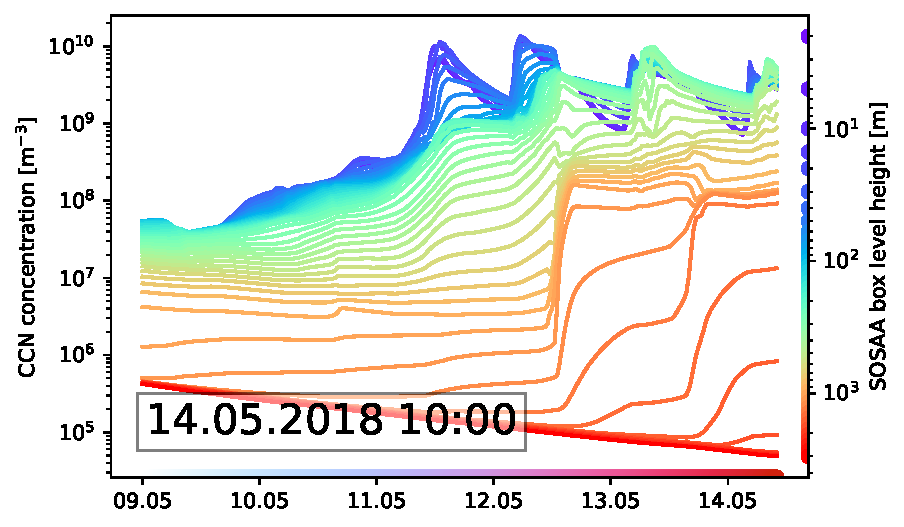
\includegraphics[width=0.49\textwidth]{sosaa-data/figures/trajectories/trajectory-14.05.2018:10.00-ccn.pdf}
    \end{subfigure}
    \begin{subfigure}
        \centering
        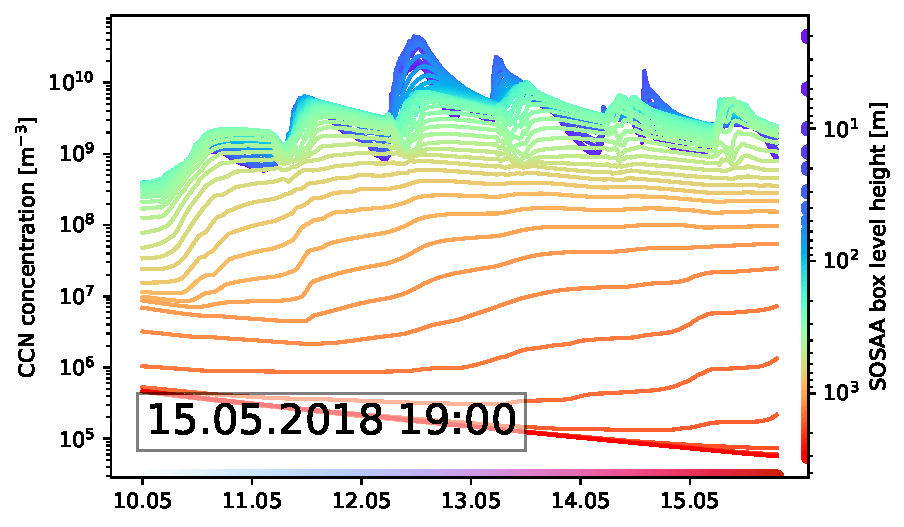
\includegraphics[width=0.49\textwidth]{sosaa-data/figures/trajectories/trajectory-15.05.2018:19.00-ccn.pdf}
    \end{subfigure}

    \begin{subfigure}
        \centering
        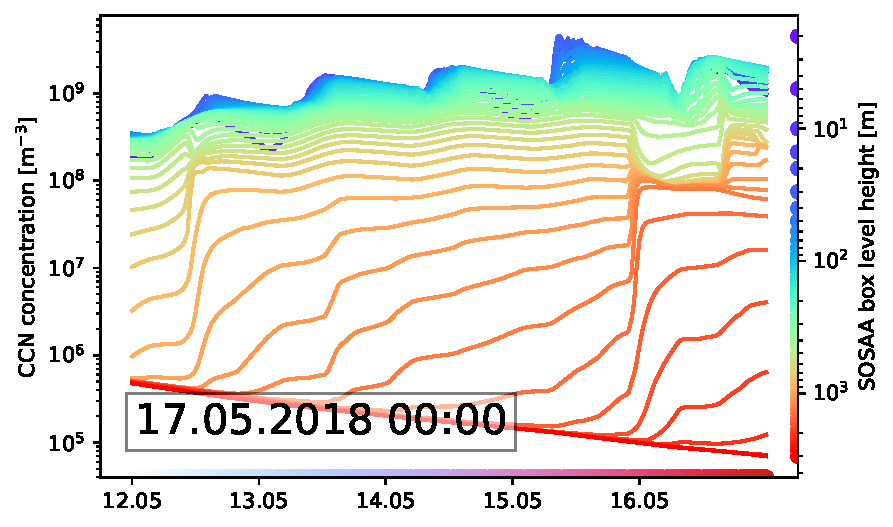
\includegraphics[width=0.49\textwidth]{sosaa-data/figures/trajectories/trajectory-17.05.2018:00.00-ccn.pdf}
    \end{subfigure}
    \begin{subfigure}
        \centering
        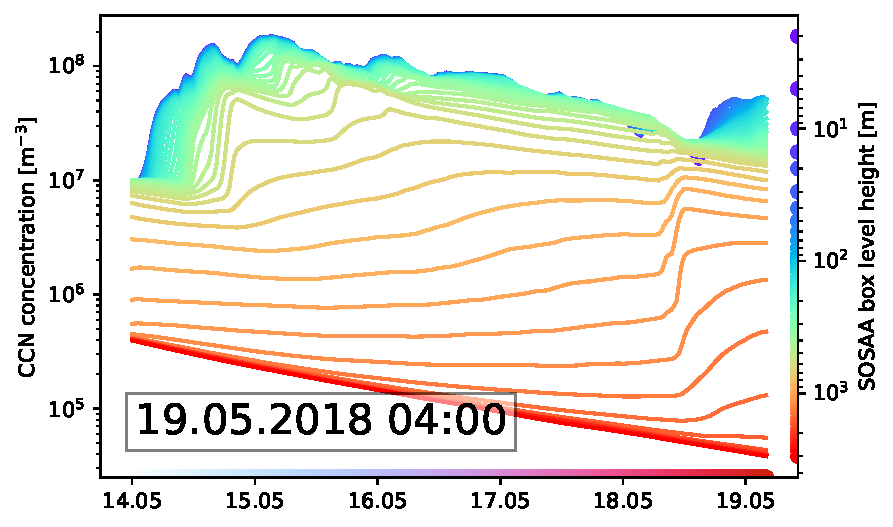
\includegraphics[width=0.49\textwidth]{sosaa-data/figures/trajectories/trajectory-19.05.2018:04.00-ccn.pdf}
    \end{subfigure}

    \begin{subfigure}
        \centering
        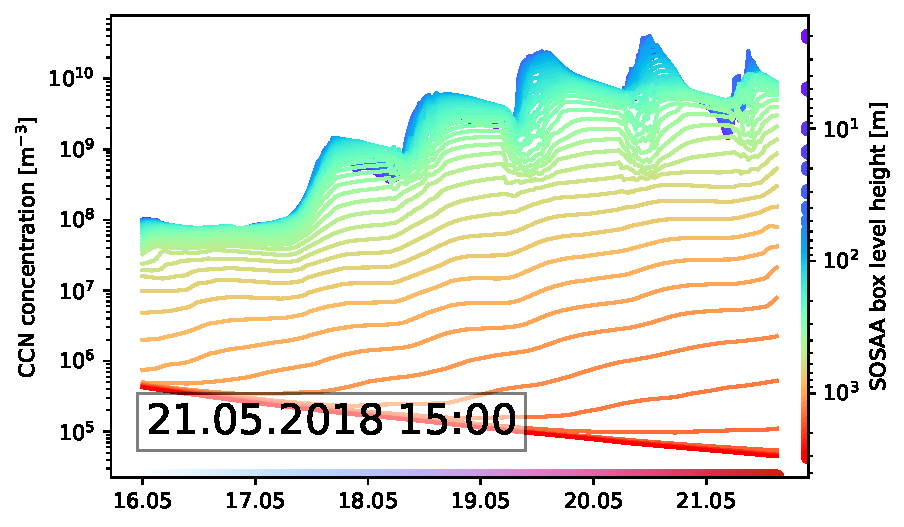
\includegraphics[width=0.49\textwidth]{sosaa-data/figures/trajectories/trajectory-21.05.2018:15.00-ccn.pdf}
    \end{subfigure}
    \begin{subfigure}
        \centering
        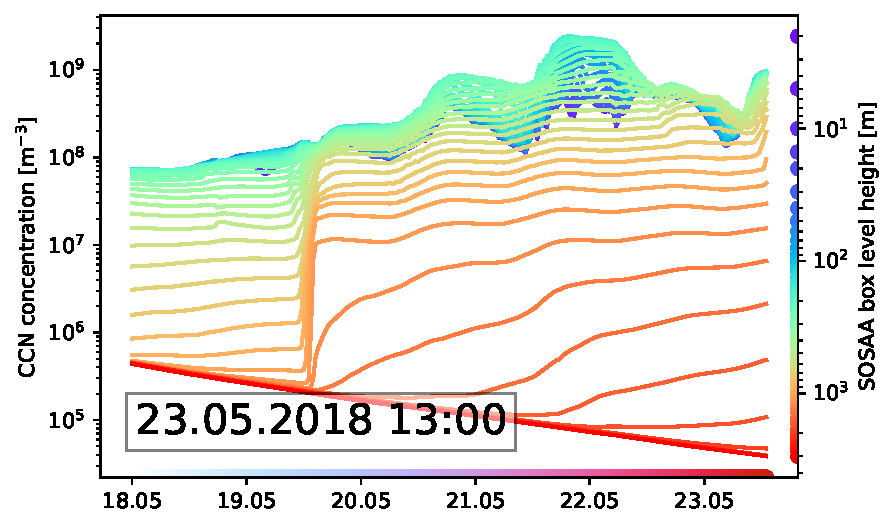
\includegraphics[width=0.49\textwidth]{sosaa-data/figures/trajectories/trajectory-23.05.2018:13.00-ccn.pdf}
    \end{subfigure}

    \caption[CCN concentration of the six example trajectories]{Per-trajectory CCN concentration over time at each of the simulated height levels. The x-axis repeats the timeline colour-coding from \Cref{fig:six-trajectories-maps}. The right y-axis shows the colour-coded height of each box level. Even though the first $48\text{h}$ are excluded for warm-up, the highest layers are still initialisation-dominated.}
    \label{fig:six-trajectories-ccn}
\end{figure}

\noindent The SOSAA simulation produces an output NetCDF file \cite{netcdf-1989} for every trajectory (see \Cref{txt:data-layout-variables}), from which we use the \texttt{dp\_dry\_fs} and \texttt{nconc\_par} variables. \texttt{dp\_dry\_fs} stores the diameter of every aerosol size-bin that SOSAA simulates. \texttt{nconc\_par} contains the number concentration for each size-bin stored for every SOSAA box height level and output time step. We count all size bins with a diameter above $80 \text{nm}$ \cite{ccn-size-2006} towards a rough estimate of the CCN concentration. \Cref{exe:ccn-concentration} below gives a sketch of the Python code to extract the CCN concentration. \Cref{fig:six-trajectories-ccn} shows the resulting CCN concentration profiles for each of the six trajectories. The height levels are spread roughly logarithmically in order to have a higher simulation resolution near the ground. Note that even though the first $48 \text{h}$ of every trajectory are used for warm-up and excluded from analysis, the highest-most layers still show after-effects from their initialisation.

\begin{listing}[H]
    \capstart % manually apply hypcap
    \begin{minted}[linenos,escapeinside=@@]{python}
import numpy as np; import pandas as pd

# Extract the CCN concentration from a SOSAA output NetCDF dataset
def get_ccn_concentration(output):
    ccn_bin_indices, = np.nonzero(output["dp_dry_fs"][:].data > 80e-9)

    return pd.DataFrame({
        "time": np.repeat(output["time"][:].data, output["lev"].shape[0]),
        "level": np.tile(output["lev"][:].data, output["time"].shape[0]),
        "ccn": np.sum(output["nconc_par"][:].data[:,ccn_bin_indices,:], axis=1).flatten(),
    }).set_index(["time", "level"])
    \end{minted}
    \caption[CCN concentration calculation procedure]{Example Python implementation of extracting the CCN concentration from the SOSAA output NetCDF file. The returned \texttt{pandas} data frame is indexed by the time step first and the height level second. The conversion from SOSAA's time format into `seconds until arrival at Hyyti\"al\"a' is omitted here for brevity.}
    \label{exe:ccn-concentration}
\end{listing}

\section{Analysing the SOSAA Input Feature Importance} \label{txt:feature-importance}

In this last section, we explore which features (see \Cref{app:sosaa-variables}) two simple machine learning models look at to make their predictions. We limit this exploration to Random Forests (see \Cref{txt:ensembles-decision-tree-random-forest}) and Pairwise Difference Regression (see \Cref{txt:padre-rf}) given their robustness with many features and little date \citeauthor{padre-rf-2021}. All feature importance experiments are evaluated by training on the combined training data from all six trajectories (see \Cref{txt:six-trajectories}) and testing on their combined validation sets. 

\begin{table}[H]
    \centering
    \begin{tabular}{ccccc} \toprule
        \multicolumn{1}{l}{} & \multicolumn{2}{c}{\textbf{Random Forest} ($MSE = 0.0012$)} & \multicolumn{2}{c}{\textbf{PADRE-RF} ($MSE = 0.156$)} \\ \cmidrule(r){2-5}
        \multicolumn{1}{c}{\textbf{emissions}} & \multicolumn{1}{c}{$\Delta MSE$} & top two $\Delta MSE$ & \multicolumn{1}{c}{$\Delta MSE$} & top two $\Delta MSE$ \\ \midrule
        \multicolumn{1}{c}{\multirow{2}{*}{\textbf{anthropogenic}}} & \multicolumn{1}{c}{$0.295$} & $0.0258$: $\text{CO}_2$ $_{(-12\text{h}, +16\text{l})}$ & \multicolumn{1}{c}{$0.22$} & $0.0264$: $\Delta$isoprene $_{(-48\text{h},+64\text{l})}$ \\
        \multicolumn{1}{c}{} & \multicolumn{1}{c}{(\#1)} & $0.0134$: pentanes $_{(-6\text{h},-8\text{l})}$ & \multicolumn{1}{c}{(\#2)} & $0.0154$: $\Delta \text{CO}_2$ $_{(-48\text{h},+64\text{l})}$ \\
        \multicolumn{1}{c}{\multirow{2}{*}{\textbf{temperature}}} & \multicolumn{1}{c}{$0.11$} & $0.0266$: temperature $_{(-48\text{h},\pm 2\text{l})}$ & \multicolumn{1}{c}{$0.355$} & $0.0887$: $\Delta$temperature $_{(-6\text{h},+8\text{l})}$ \\
        \multicolumn{1}{c}{} & \multicolumn{1}{c}{(\#2)} & $0.0064$: temperature $_{(-12\text{h},+16\text{l})}$ & \multicolumn{1}{c}{(\#1)} & $0.0706$: $\Delta$temperature $_{(-24\text{h},+32\text{l})}$ \\
        \multicolumn{1}{c}{\multirow{2}{*}{\textbf{anthr. $\text{NO}_{x}$}}} & \multicolumn{1}{c}{$0.0643$} & $0.0588$: $\text{NO}_{x}$ $_{(-12\text{h},+16\text{l})}$ & \multicolumn{1}{c}{$0.08$} & $0.0342$: $\text{NO}_{x}$ $_{(-48\text{h},+64\text{l})}$ \\
        \multicolumn{1}{c}{} & \multicolumn{1}{c}{(\#3)} & $0.0003$: $\text{NO}_{x}$ $_{(-6\text{h},-8\text{l})}$ & \multicolumn{1}{c}{(\#3)} & $0.0041$: $\Delta\text{NO}_{x}$ $_{(-48\text{h},+64\text{l})}$ \\
        \multicolumn{1}{c}{\multirow{2}{*}{\textbf{aerosols}}} & \multicolumn{1}{c}{$0.0147$} & $0.001$: $400$-$1000\text{nm}$ $_{(-48\text{h},-64\text{l})}$ & \multicolumn{1}{c}{$0.0677$} & $0.0106$: $\Delta 50$-$70\text{nm}$ $_{(-48\text{h},+64\text{l})}$ \\
        \multicolumn{1}{c}{} & \multicolumn{1}{c}{(\#4)} & $0.0008$: $10$-$20\text{nm}$ $_{(-6\text{h},-8\text{l})}$ & \multicolumn{1}{c}{(\#4)} & $0.0017$: $\Delta 400$-$1000\text{nm}$ $_{(-48\text{h},+64\text{l})}$ \\
        \multicolumn{1}{c}{\multirow{2}{*}{\textbf{anthr. $\text{SO}_{2}$}}} & \multicolumn{1}{c}{$0.0102$} & $0.0078$: $\text{SO}_{2}$ $_{(-12\text{h},+16\text{l})}$ & \multicolumn{1}{c}{$0.0621$} & $0.0081$: $\text{SO}_{2}$ $_{(-12\text{h},+16\text{l})}$ \\
        \multicolumn{1}{c}{} & \multicolumn{1}{c}{(\#5)} & $0.0003$: $\text{SO}_{2}$ $_{(-6\text{h},-8\text{l})}$ & \multicolumn{1}{c}{(\#6)} & $0.0027$: $\Delta \text{SO}_{2}$ $_{(-48\text{h},+64\text{l})}$ \\
        \multicolumn{1}{c}{\multirow{2}{*}{\textbf{biogenic}}} & \multicolumn{1}{c}{$0.0031$} & $0.0002$: $\text{CH}_2\text{O}$ $_{(-48\text{h},\pm 2\text{l})}$ & \multicolumn{1}{c}{$0.0635$} & $0.0043$: MBO $_{(-24\text{h},-32\text{l})}$ \\
        \multicolumn{1}{c}{} & \multicolumn{1}{c}{(\#6)} & $0.0001$: aldehydes $_{(-48\text{h},-64\text{l})}$ & \multicolumn{1}{c}{(\#5)} & $0.0026$: $\Delta\text{CH}_{3}\text{CHO}$ $_{(-24\text{h},-32\text{l})}$ \\
        \multicolumn{1}{c}{\multirow{2}{*}{\textbf{monoterpenes}}} & \multicolumn{1}{c}{$0.0018$} & $0.0004$: $\alpha$-pinene $_{(-48\text{h},-64\text{l})}$ & \multicolumn{1}{c}{$0.0564$} & $0.0004$: $\alpha$-pinene $_{(-24\text{h},\pm 2\text{l})}$ \\
        \multicolumn{1}{c}{} & \multicolumn{1}{c}{(\#7)} & $0.0001$: $\beta$-pinene $_{(-48\text{h},-64\text{l})}$ & \multicolumn{1}{c}{(\#7)} & $0.0002$: $\Delta \beta$-pinene $_{(-1.5\text{h},+0\text{l})}$ \\
        \multicolumn{1}{c}{\multirow{2}{*}{\textbf{sesquiterpenes}}} & \multicolumn{1}{c}{$0.0014$} & $0.0002$: sqtrps $_{(-48\text{h},-64\text{l})}$ & \multicolumn{1}{c}{$0.0554$} & $0.0001$: $\Delta$sqtrps $_{(-6\text{h},\pm 1\text{l})}$ \\
        \multicolumn{1}{c}{} & \multicolumn{1}{c}{(\#8)} & $0.0001$: sqtrps $_{(-48\text{h},\pm 2\text{l})}$ & \multicolumn{1}{c}{(\#8)} & $0.0001$: sqtrps $_{(-48\text{h},-64\text{l})}$ \\
        \multicolumn{1}{c}{\multirow{2}{*}{\textit{\textbf{ungrouped}}}} & \multicolumn{1}{c}{\multirow{2}{*}{--}} & $0.0203$: SSR $_{(-48\text{h},\pm 2\text{l})}$ & \multicolumn{1}{c}{\multirow{2}{*}{--}} & $0.0283$: $\Delta$DMS $_{(-24\text{h},-32\text{l})}$ \\
        \multicolumn{1}{c}{} & \multicolumn{1}{c}{} & $0.0113$: $\text{CH}_4$ $_{(-6\text{h},-8\text{l})}$ & \multicolumn{1}{c}{} & $0.0154$: $\Delta q_{met}$ $_{(-6\text{h},+8\text{l})}$ \\ \bottomrule
    \end{tabular}
    \caption[Permutation Feature Importance for Random Forests and PADRE-RF]{Permutation Feature Importance for Random Forests and PADRE-RF as measured by the increase in the mean-squared error. The permutations are performed both in the perturbations groups from \Cref{txt:perturbation-generalisation} and on a per-feature basis. For each group, the top two individual features are listed as well.}
    \label{tab:permutation-feature-importance}
\end{table}

\noindent First, we evaluate the \textbf{permutation importance} of each post-space-time expansion feature by shuffling the values of one feature and recording the performance drop. Features that are integral to a trained model are expected to be associated with a higher drop in prediction performance.

\Cref{tab:permutation-feature-importance} lists the permutation importances of the perturbation groups from \Cref{txt:perturbation-generalisation} and top two most important features in each group. To save space, the space-time-expanded features from \Cref{txt:space-time-expansion} are written with just their lower time bound and outer height level bound. For instance, $\text{NO}_{x}$ $_{(-6\text{h},-8\text{l})}$ refers to the averaged $\text{NO}_{x}$ emissions that occurred between $6\text{h}$ and $3\text{h}$ before the current time step and within all height layers starting two below the current layer and expanding down up to eight layers below. Note that since SOSAA is usually run with around $50$ height layers, any features using, e.g. $+64\text{l}$ effectively include all height layers above the current one. Please refer back to \Cref{txt:space-time-expansion} for details on the space-time expansion of all features.

First, we notice that anthropogenic emissions and air temperature are the most important, followed by anthropogenic $\text{NO}_{x}$ emissions. Second, the importance order of perturbation groups is almost the same for both Random Forests and PADRE-RF, apart from anthropogenic and temperature as well as $\text{SO}_2$ and biogenics switching ranks. Note that low perturbation importance does not necessarily mean that this feature has low relevance in the real world. For instance, the lower importance of all biogenic emissions may also be related to the lower variation in these inputs across the dataset (see \Cref{fig:trajectory-inputs-14-05}, \Cref{fig:trajectory-inputs-15-05}, and \Cref{fig:trajectory-inputs-17-05}). Third, we notice that since biogenic emissions occur near the ground, features that look at a large range of height layers below have high importance. In contrast, the models assign high importance to averaging all anthropogenic emissions in height layers above the current one. Fourth, we can see that PADRE-RF has a less steep drop-off in importance, especially for biogenic, monoterpene, and sesquiterpene emissions. Thus, we hypothesise that PADRE-RF may have a higher capacity than Random Forests at predicting changes in CCN concentrations for perturbations of these groups. This hypothesis is tested in \Cref{txt:perturbation-generalisation}.

\newpar Second, we investigate the minimal set of features needed to achieve good predictive performance. In particular, we look for the smallest set of features such that adding a new feature no longer brings an improvement that exceeds a set threshold, here $\Delta MSE_{min} = -0.01$. In this sequential feature selection process, we first train one model per feature and then choose the feature with the lowest prediction error, evaluated using $k$-fold cross-validation. Next, we iterate over all remaining features and check which second feature can be selected to produce the best two-feature model. Since Random Forests can be very accurate with very few features by overfitting on noise in the data, we instead use linear regression models in this investigation. In order to still capture non-linear processes, we expand the selected features to their third-order polynomial combinations. To avoid the $\text{O}(F^3)$ complexity for $F$ features, we approximate this polynomial expansion with just $4F$ features using the Nystr\"om method \cite{nystroem-kernel-2000, nystroem-fourier-2012}, as implemented in the \texttt{scikit-learn} library \cite{scikit-learn-2011}.

\newpar Training on the standard features, sequential feature selection selects the following features with $MSE = 0.321$:
\begin{flalign*}
    \quad \{ \quad & && \\
    & \text{temperature }_{(-24\text{h},+32\text{l})}, \text{temperature }_{(-24\text{h},-32\text{l})}, \text{temperature }_{(-6\text{h},+8\text{l})}, \text{temperature }_{(-12\text{h},+16\text{l})}, && \\
    & \text{anthropogenic NH}_{3}\text{ }_{(-24\text{h},-32\text{l})}, \text{aerosols } 200\text{-}400\text{nm }_{(-24\text{h},-32\text{l})}, && \\
    \quad \} \quad & &&
\end{flalign*}
In comparison, the following pairwise difference regression features are chosen with $MSE = 0.527$:
\begin{flalign*}
    \quad \{ \quad & && \\
    & \Delta \text{temperature }_{(-24\text{h},+32\text{l})}, \text{temperature }_{(-48\text{h},+64\text{l})}, \text{temperature }_{(-24\text{h},-32\text{l})}, && \\
    & \Delta \text{biogenic isoprene }_{(-3\text{h},-4\text{l})}, \Delta \text{temperature }_{(-24\text{h},-32\text{l})}, \Delta \text{temperature }_{(-48\text{h},-64\text{l})}, && \\
    & \Delta \text{biogenic CO }_{(-3\text{h},-4\text{l})}, \Delta \text{biogenic CO }_{(-3\text{h},+4\text{l})}, && \\
    \quad \} \quad & &&
\end{flalign*}
We can see that, unlike permutation importance, sequential feature selection identifies temperature as the most important feature. In fact, the temperature features create the most significant reductions in the prediction error for both Random Forests and Pairwise Difference Regression. In contrast, the later-selected features only provide more minor improvements that do not significantly exceed the $\Delta MSE_{min} = -0.01$ threshold. One possible explanation might be that temperature is a dominant variable. In this case, temperature perturbations should have the largest impact on CCN concentrations in \Cref{txt:perturbation-generalisation}. The Icarus RSM should predict both temperature and other perturbations well, the latter simply because they would not have a significant impact. However, it is also possible that temperature simply is the only variable that has significant independent variation within the dataset. In this case, the Icarus RSM would succeed in predicting temperature perturbations but fail at predicting the change in CCN for other perturbations.


    %% OOD Detection, Synthesis and Scoring Experiments
    \chapter{Exploring Out-of-Distribution Detection} \label{txt:ood-detection-chapter}

Detecting out-of-distribution inputs is a critical component of the Icarus-RSM architecture introduced in \Cref{txt:icarus-rsm}. Without OOD detection, an RSM that has been trained on insufficient data may make predictions even on unseen inputs that lie entirely outside its training data space and for which the model thus \textbf{cannot} make any prediction. This chapter explores three crucial aspects of OOD detection: methods for identifying novel inputs (\Cref{txt:ood-detection-comparison}), techniques to synthesise OOD inputs for supervised training methods (\Cref{txt:ood-synthesis-analysis}), and approaches to assign meaningful prediction confidence scores (\Cref{txt:confidence-scoring-comparison}). Thus, this chapter aims to provide an overview and give recommendations (\Cref{txt:ood-recommendations}) for OOD detection in the Icarus-RSM.

\section{Toy-Comparisons of Novelty Detection Methods} \label{txt:ood-detection-comparison}

\Cref{txt:novelty-detection} has summarised several methods for novelty detection. The following section visually evaluates several of these methods, which are implemented using the \texttt{scikit-learn} library \cite{scikit-learn-2011}. In the following figures, each row showcases one method, while the three columns contain the following three test cases:
\begin{enumerate}
    \item Two groups of training points are scattered along a line in the 2D feature space. The target variable only depends on the location along the line. In this example, points off the line are OOD.
    \item The training points are scattered around the sine-displaced boundary of a circle, but none are inside it. The target variable only depends on the location along the boundary. Again, points off the line are OOD.
    \item The training points are sampled from a 10-dimensional multivariate normal distribution, where one of the features is set to a constant. This example tests whether an OOD detection method can find a needle in a high-dimensional haystack, i.e. identify that points which do not share the constant are OOD.
\end{enumerate}
In these examples, the OOD detection score is transformed into a confidence level representing the percentage of validation data inputs with greater or equal ID scores (see \Cref{eq:dime-id-percentile}). Thus, even ID inputs may have a low confidence score, but OOD inputs should never obtain a high confidence score. All plots encode the confidence level from $c = 0.0$ for OOD inputs in black, over blue and green, to $c = 1.0$ for ID inputs in yellow using the CET-L20 colour map \cite{color-cet-2015, color-cet-2023}. The first two plots depict a subset of the training points using black $\texttt{x}$ markers. Note that the first two plots do not have axis labels since the two axes map directly to the 2D feature space axes. The third plot differs and shows the \textit{distribution} of confidence values on the y-axis for different x-axis values for the constant-in-training feature. The constant value is highlighted as a white line.

\begin{figure}[H]
    \centering
    \begin{subfigure}
        \centering
        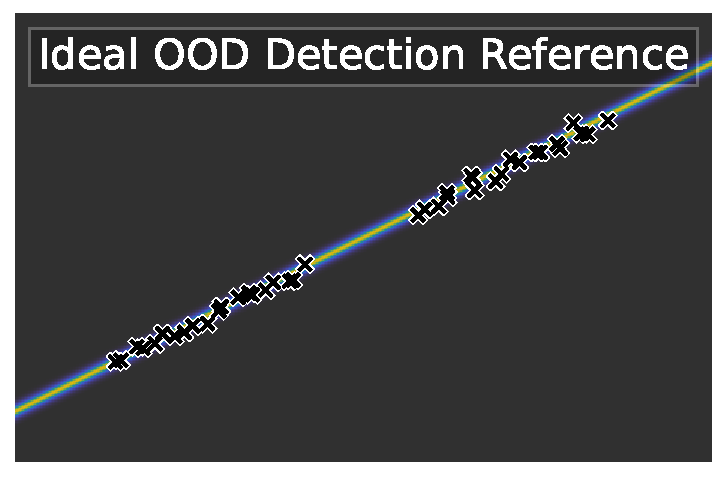
\includegraphics[width=0.388\textwidth,valign=t]{ood-detection/figures/ood-detection/confidence-line-aa-optimal.pdf}
    \end{subfigure}
    \begin{subfigure}
        \centering
        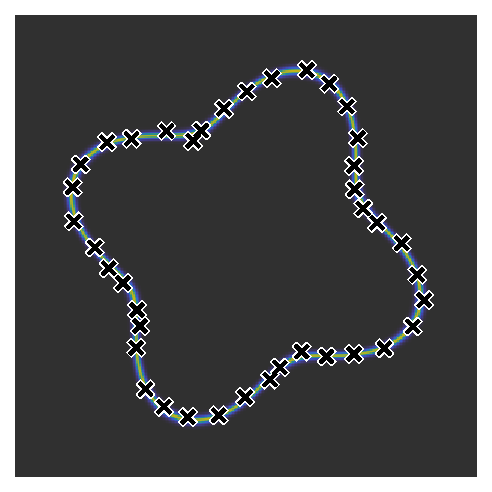
\includegraphics[width=0.254\textwidth,valign=t]{ood-detection/figures/ood-detection/confidence-circle-aa-optimal.pdf}
    \end{subfigure}
    \begin{subfigure}
        \centering
        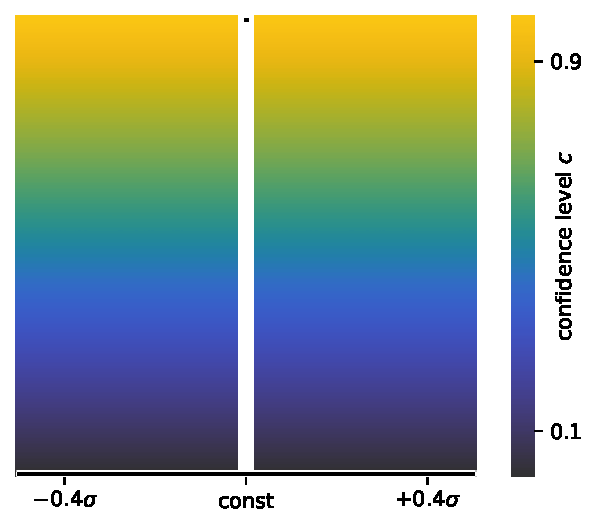
\includegraphics[width=0.308\textwidth,valign=t]{ood-detection/figures/ood-detection/confidence-haystack-aa-optimal.pdf}
    \end{subfigure}

    \vspace{-0.25em}
    \caption[Reference Example of one ideal OOD Detector]{By-example (see \Cref{txt:ood-detection-comparison}) evaluation of one possible ideal OOD detection method.}
    \label{fig:ideal-ood-detection}
\end{figure}

\noindent Let us start by comparing what these plots could look like for an ideal OOD detector with one-class SVM, an unsupervised classification method first described in \textcite{ood-svm-1999}. This method trains a support vector machine on ID inputs, assigning them a positive score, while OOD inputs get a negative score. In \Cref{fig:ideal-ood-detection}, we can see that our interpretation of an ideal OOD detector is able to succinctly extract the line and circle boundary ID subspaces in the first two figures. Note that the lines look very thin since the percentile-based confidence score from \Cref{eq:dime-id-percentile} uniformly spreads the confidence values across all ID inputs. In contrast, the washed-out two-hill confidence map in \Cref{fig:one-class-ood-detection} shows that one-class SVM only recognises that two groups of ID points are given but not that only points along that line should have high confidence. For the middle circle example, it incorrectly classifies most of the full circle as ID, even though the training data only lies on its boundary. Finally, in the haystack example, our ideal OOD detector assigns high confidence only to inputs that have the same feature value as the constant seen in training. Specifically, there is only a single black high-confidence dot on the white constant line. One-class SVM instead spreads its confidence values uniformly, meaning it is unable to identify the haystack as OOD.

\begin{figure}[H]
    \centering
    \begin{subfigure}
        \centering
        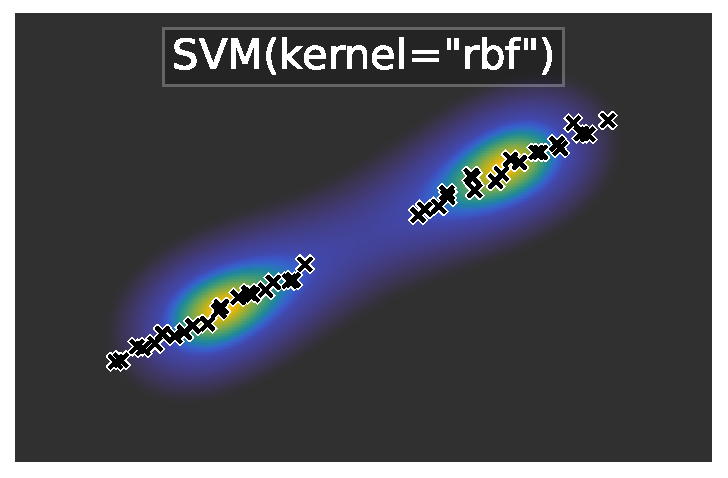
\includegraphics[width=0.388\textwidth,valign=t]{ood-detection/figures/ood-detection/confidence-line-svm-rbf.pdf}
    \end{subfigure}
    \begin{subfigure}
        \centering
        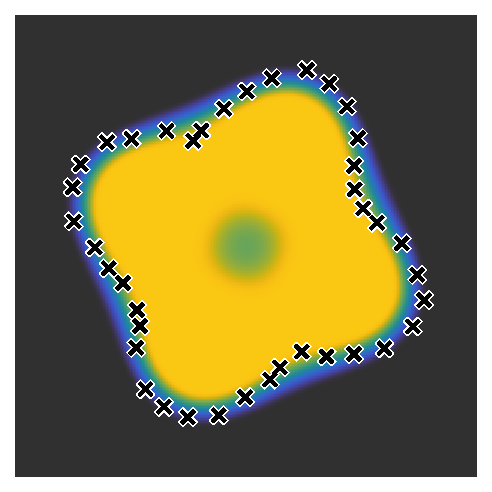
\includegraphics[width=0.254\textwidth,valign=t]{ood-detection/figures/ood-detection/confidence-circle-svm-rbf.pdf}
    \end{subfigure}
    \begin{subfigure}
        \centering
        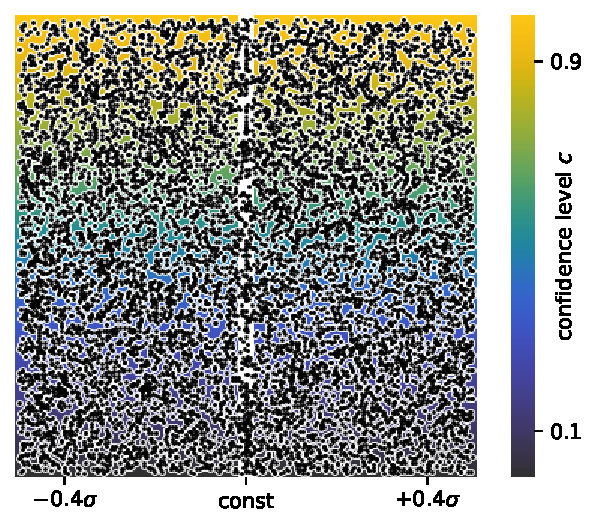
\includegraphics[width=0.308\textwidth,valign=t]{ood-detection/figures/ood-detection/confidence-haystack-svm-rbf.pdf}
    \end{subfigure}

    \caption[The One-class SVM OOD detection method]{By-example (see \Cref{txt:ood-detection-comparison}) evaluation of the One-class SVM \cite{ood-svm-1999} OOD detection method.}
    \label{fig:one-class-ood-detection}
\end{figure}

\subsection{Distance- and Isolation-based Methods}

The Mahalanobis distance (see \Cref{eq:mahalanobis-distance}) treats the ID data as a multivariate Gaussian random variable and measures how much the unseen data deviates from it. \Cref{fig:md-lof-ood-detection} shows that while this method fits the line data well (by squeezing an ellipsoid decision boundary around it), it fails for the circle and haystack test cases.

\begin{figure}[H]
    \centering
    \begin{subfigure}
        \centering
        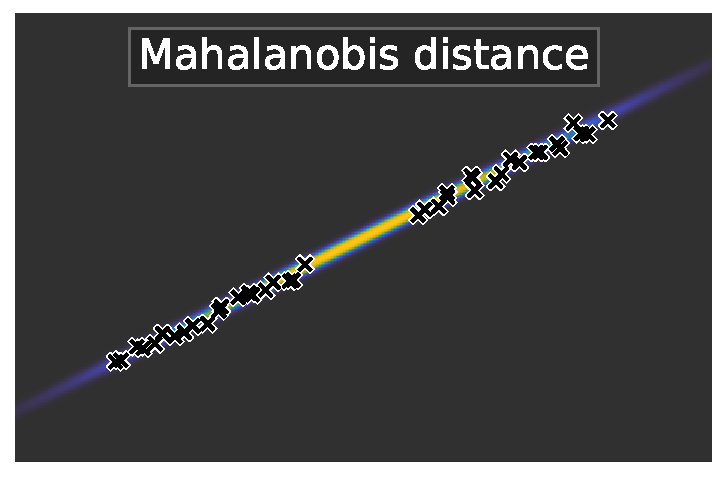
\includegraphics[width=0.388\textwidth,valign=t]{ood-detection/figures/ood-detection/confidence-line-mahalanobis.pdf}
    \end{subfigure}
    \begin{subfigure}
        \centering
        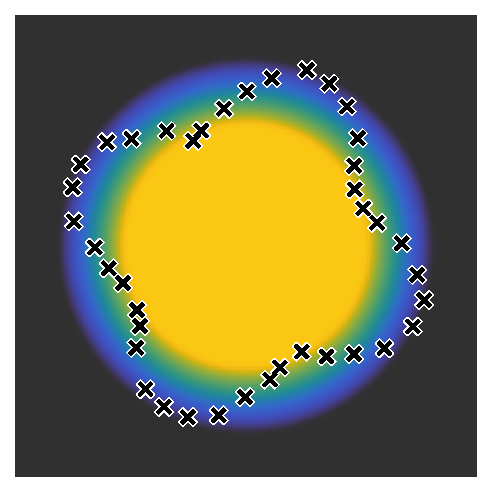
\includegraphics[width=0.254\textwidth,valign=t]{ood-detection/figures/ood-detection/confidence-circle-mahalanobis.pdf}
    \end{subfigure}
    \begin{subfigure}
        \centering
        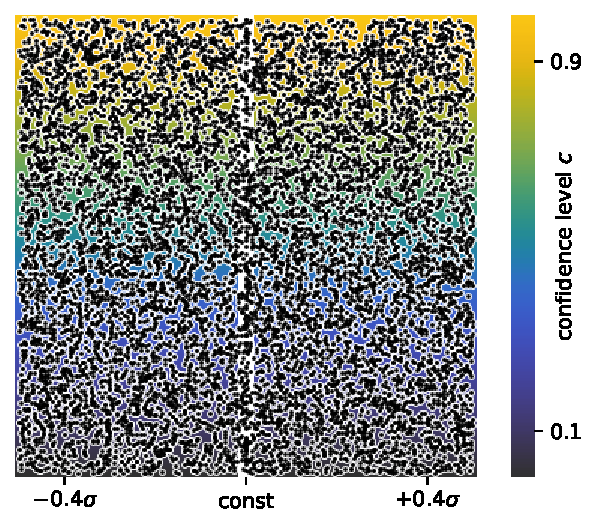
\includegraphics[width=0.308\textwidth,valign=t]{ood-detection/figures/ood-detection/confidence-haystack-mahalanobis.pdf}
    \end{subfigure}

    \begin{subfigure}
        \centering
        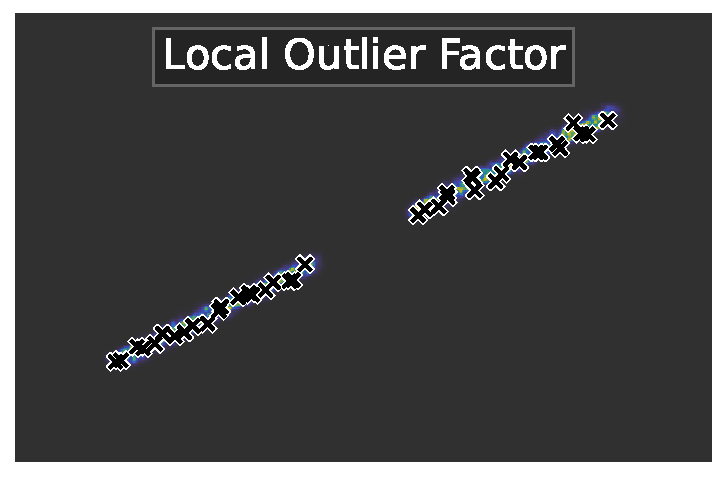
\includegraphics[width=0.388\textwidth,valign=t]{ood-detection/figures/ood-detection/confidence-line-lof.pdf}
    \end{subfigure}
    \begin{subfigure}
        \centering
        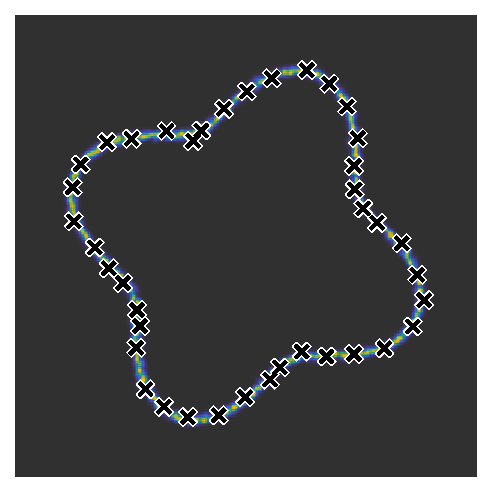
\includegraphics[width=0.254\textwidth,valign=t]{ood-detection/figures/ood-detection/confidence-circle-lof.pdf}
    \end{subfigure}
    \begin{subfigure}
        \centering
        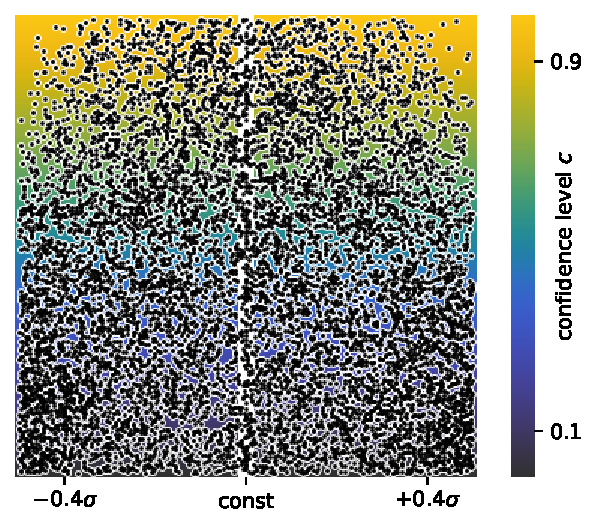
\includegraphics[width=0.308\textwidth,valign=t]{ood-detection/figures/ood-detection/confidence-haystack-lof.pdf}
    \end{subfigure}

    \caption[Distance-based OOD detection methods]{By-example (see \Cref{txt:ood-detection-comparison}) evaluation of the Mahalanobis distance (see \Cref{eq:mahalanobis-distance}) and the Local Outlier Factor (see \Cref{txt:ood-distance}) as distance-based OOD detection methods.}
    \label{fig:md-lof-ood-detection}
\end{figure}

\noindent The Local Outlier Factor (LOF, see \Cref{txt:ood-distance}) estimates the training data density around unseen data. Thus, it performs much better on the line and circle examples where the data points are closely scattered. Unlike the prior methods, the LOF classifies the gap between the two groups on the line as OOD, which may be too conservative if we assume that a machine-learning model can interpolate between the two groups. LOF is also the first method that produces slightly lower confidence for the OOD inputs in the haystack.

Isolation Forests are a non-distance-based OOD detection method by \textcite{isolation-forest-2008} and \textcite{isolation-forest-2012} that uses a forest of binary trees with random splits. OOD inputs are detected as isolated since they require fewer splits to reach a tree leaf node where they are isolated from ID inputs. Unfortunately, \Cref{fig:if-ood-detection} shows that Isolation Forests generate washed-out confidence patterns and fail for the haystack.

\begin{figure}[H]
    \centering
    \begin{subfigure}
        \centering
        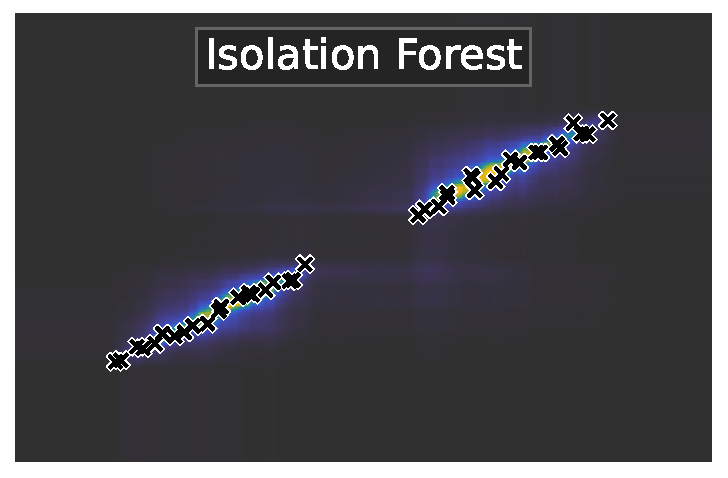
\includegraphics[width=0.388\textwidth,valign=t]{ood-detection/figures/ood-detection/confidence-line-isolation.pdf}
    \end{subfigure}
    \begin{subfigure}
        \centering
        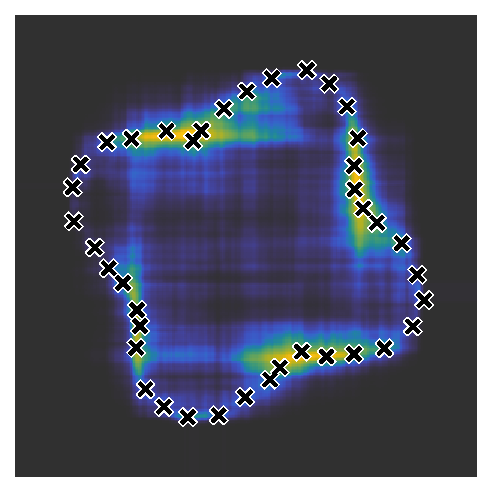
\includegraphics[width=0.254\textwidth,valign=t]{ood-detection/figures/ood-detection/confidence-circle-isolation.pdf}
    \end{subfigure}
    \begin{subfigure}
        \centering
        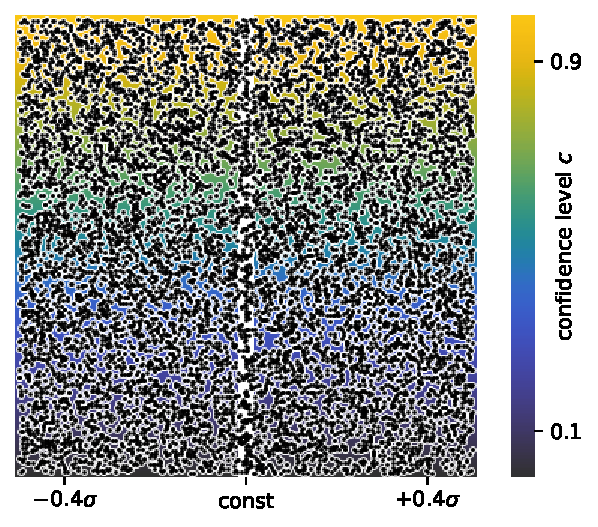
\includegraphics[width=0.308\textwidth,valign=t]{ood-detection/figures/ood-detection/confidence-haystack-isolation.pdf}
    \end{subfigure}

    \caption[Isolation Forests as an OOD detection method]{By-example (see \Cref{txt:ood-detection-comparison}) evaluation of Isolation Forests \cite{isolation-forest-2008, isolation-forest-2012} as an OOD detection method.}
    \label{fig:if-ood-detection}
\end{figure}

\subsection{Truncated PCA as a Cheap Linear Auto-Associative Method} \label{txt:truncated-pca}

In the truncated PCA method, the $d$-dimensional input data is projected onto its first $k$ principal components, where $k < d$ and chosen such that at least $95\%$ of the variance is retained. If an input can only be reconstructed from this truncated form with high error, it is OOD. \Cref{fig:truncated-pca-ood-detection} shows that the method successfully learns the line ID subspace. However, it fails in the circular example since there is no linear mapping from the 2D circle to the truncated 1st PC. In the haystack, truncated PCA displays a gradual drop in confidence for OOD inputs.

\begin{figure}[H]
    \centering
    \begin{subfigure}
        \centering
        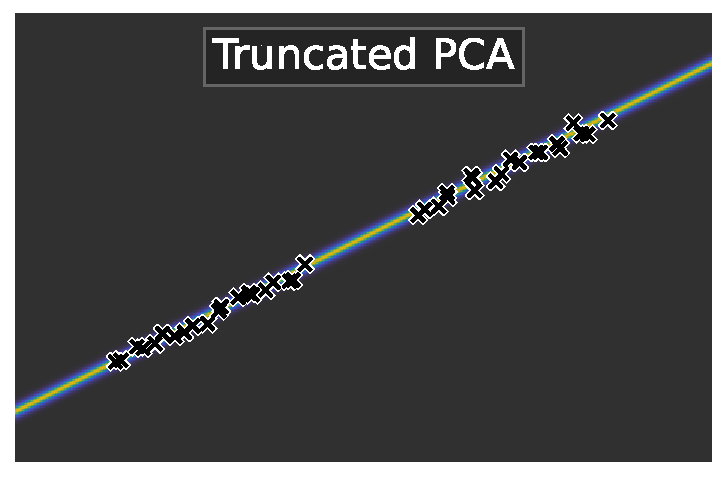
\includegraphics[width=0.388\textwidth,valign=t]{ood-detection/figures/ood-detection/confidence-line-truncated-pca.pdf}
    \end{subfigure}
    \begin{subfigure}
        \centering
        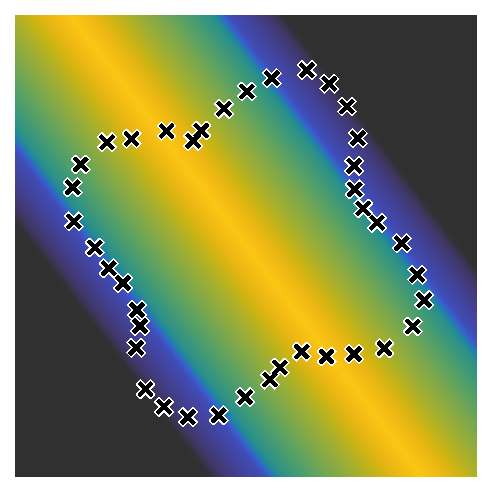
\includegraphics[width=0.254\textwidth,valign=t]{ood-detection/figures/ood-detection/confidence-circle-truncated-pca.pdf}
    \end{subfigure}
    \begin{subfigure}
        \centering
        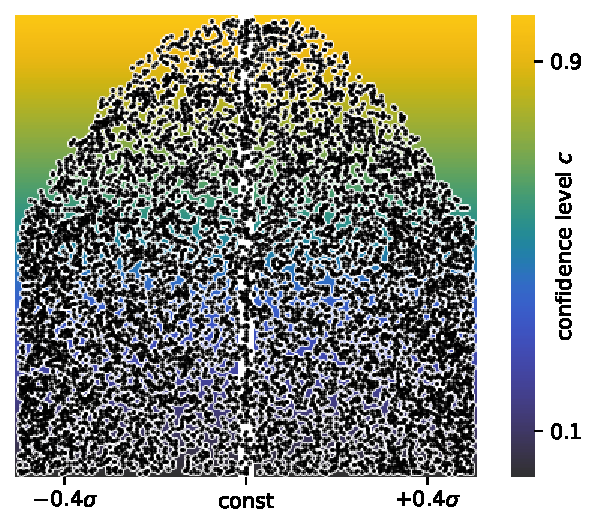
\includegraphics[width=0.308\textwidth,valign=t]{ood-detection/figures/ood-detection/confidence-haystack-truncated-pca.pdf}
    \end{subfigure}

    \caption[Truncated PCA as an OOD detection method]{By-example (see \Cref{txt:ood-detection-comparison}) evaluation of truncated PCA as an OOD detection method.}
    \label{fig:truncated-pca-ood-detection}
\end{figure}

\subsection{Exploration of diverse Auto-Associative Methods} \label{txt:ood-detection-analyis-auto-associative}

Auto-Associative Networks (see \Cref{txt:auto-associative}) are non-linear neural networks that compress and reconstruct their input. High reconstruction errors can be used as an indicator for OOD inputs. \Cref{fig:auto-associative-ood-detection} shows how auto-associative networks using the ReLU (popular) and sigmoid (recommended by \textcite{auto-associative-2001}) activation functions perform when the encoding and decoding layers have 16 neurons, and the bottleneck has one or eight for the 2D and haystack examples, respectively. While the ReLU function performs well for the haystack, it produces harsh artefacts for the circle. The sigmoid function also fails here with a solid bean shape but works for the line. As suggested by \textcite{dime-detector-2021}, we also try applying the Mahalanobis distance to the per-feature reconstruction errors instead of summing them. As shown in \Cref{fig:auto-associative-mahalanobis-ood-detection}, this produces much tighter OOD detection bounds that benefit the sigmoid activation and the haystack example, in particular.

\begin{figure}[H]
    \centering
    \begin{subfigure}
        \centering
        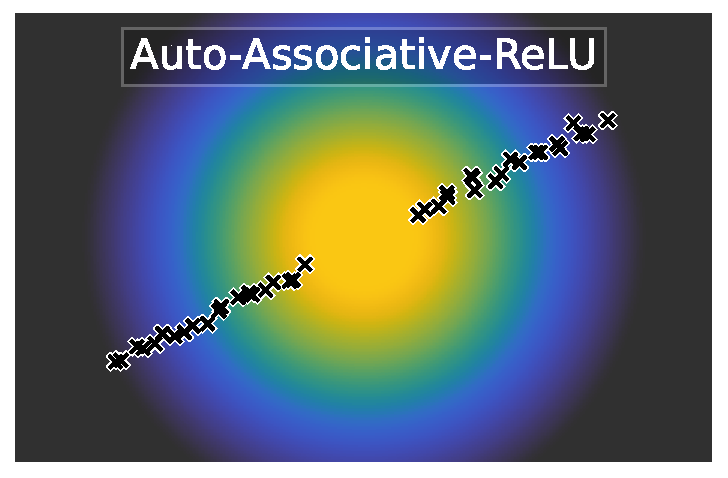
\includegraphics[width=0.388\textwidth,valign=t]{ood-detection/figures/ood-detection/confidence-line-aa-relu.pdf}
    \end{subfigure}
    \begin{subfigure}
        \centering
        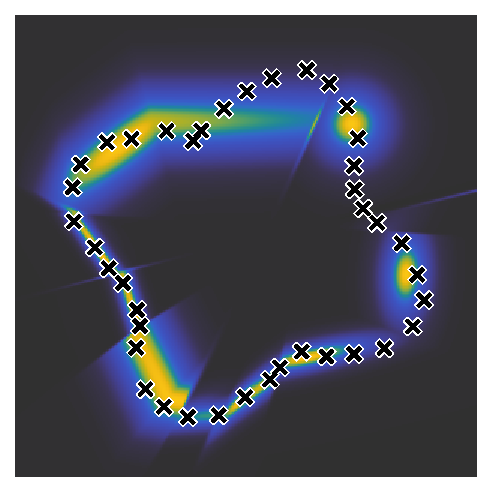
\includegraphics[width=0.254\textwidth,valign=t]{ood-detection/figures/ood-detection/confidence-circle-aa-relu.pdf}
    \end{subfigure}
    \begin{subfigure}
        \centering
        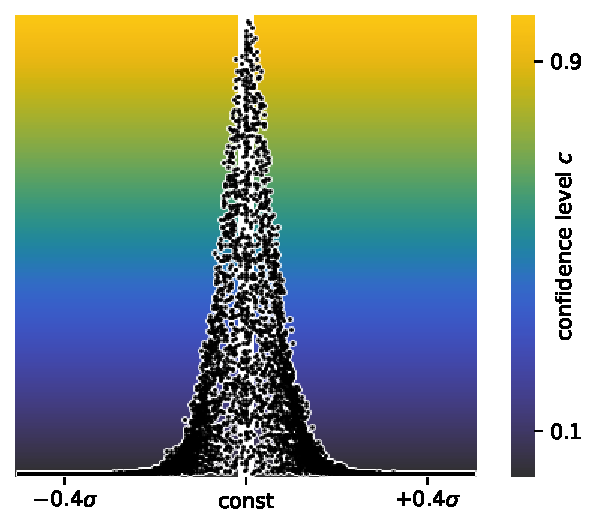
\includegraphics[width=0.308\textwidth,valign=t]{ood-detection/figures/ood-detection/confidence-haystack-aa-relu.pdf}
    \end{subfigure}

    \begin{subfigure}
        \centering
        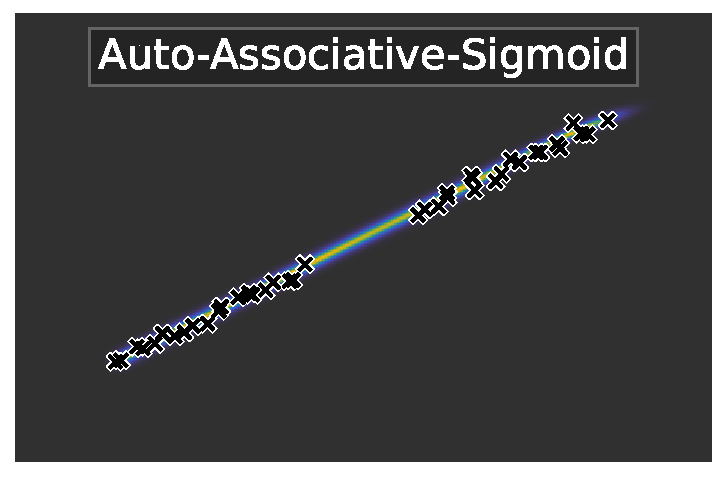
\includegraphics[width=0.388\textwidth,valign=t]{ood-detection/figures/ood-detection/confidence-line-aa-sigmoid.pdf}
    \end{subfigure}
    \begin{subfigure}
        \centering
        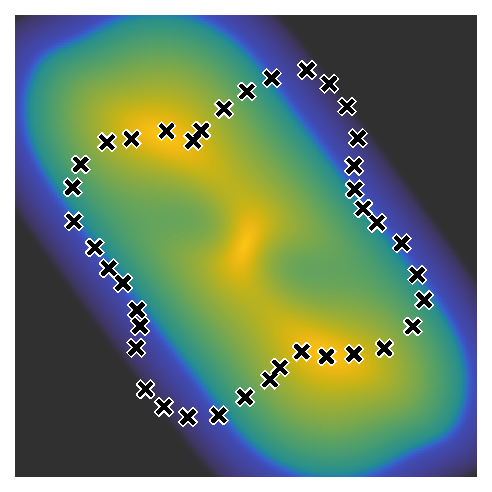
\includegraphics[width=0.254\textwidth,valign=t]{ood-detection/figures/ood-detection/confidence-circle-aa-sigmoid.pdf}
    \end{subfigure}
    \begin{subfigure}
        \centering
        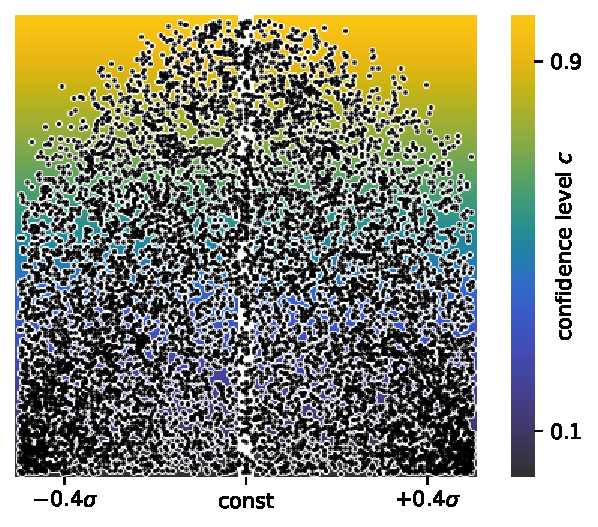
\includegraphics[width=0.308\textwidth,valign=t]{ood-detection/figures/ood-detection/confidence-haystack-aa-sigmoid.pdf}
    \end{subfigure}

    \caption[Comparison of Auto-Associative Networks as OOD detection methods]{By-example (see \Cref{txt:ood-detection-comparison}) evaluation of Auto-Associative networks (see \Cref{txt:auto-associative}) as OOD detection methods. The networks are trained with the ReLU or sigmoid activation function, and their per-feature squared reconstruction errors are summed before being transformed into a confidence score.}
    \label{fig:auto-associative-ood-detection}
\end{figure}

\begin{figure}[H]
    \centering
    \begin{subfigure}
        \centering
        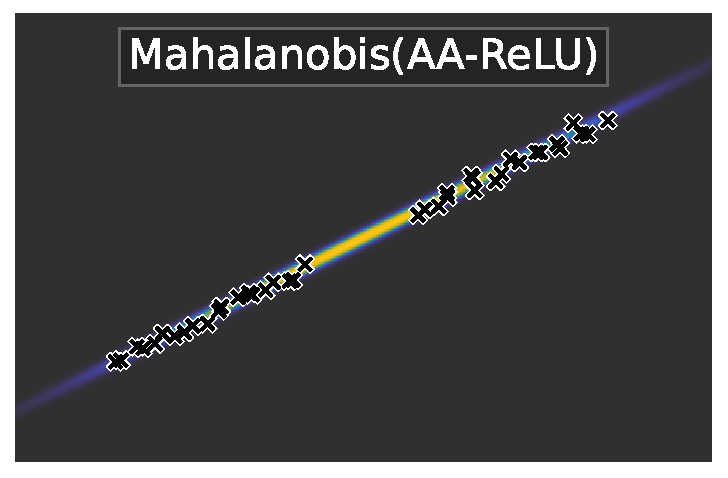
\includegraphics[width=0.388\textwidth,valign=t]{ood-detection/figures/ood-detection/confidence-line-aa-relu-mahalanobis.pdf}
    \end{subfigure}
    \begin{subfigure}
        \centering
        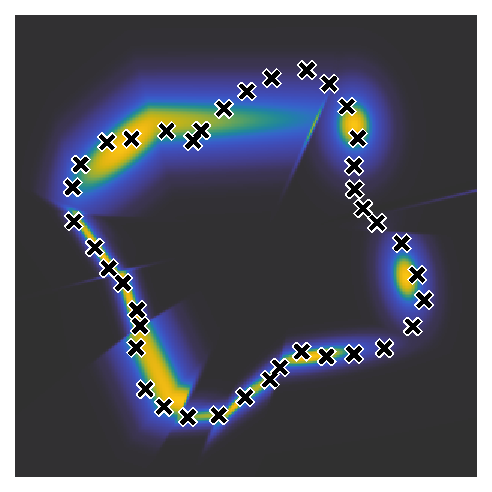
\includegraphics[width=0.254\textwidth,valign=t]{ood-detection/figures/ood-detection/confidence-circle-aa-relu-mahalanobis.pdf}
    \end{subfigure}
    \begin{subfigure}
        \centering
        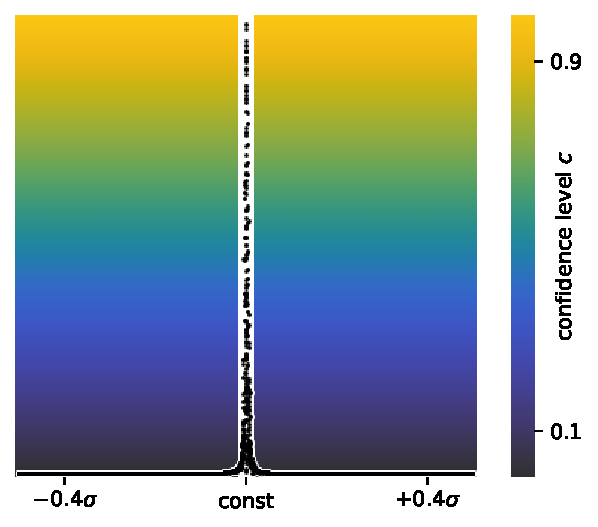
\includegraphics[width=0.308\textwidth,valign=t]{ood-detection/figures/ood-detection/confidence-haystack-aa-relu-mahalanobis.pdf}
    \end{subfigure}

    \begin{subfigure}
        \centering
        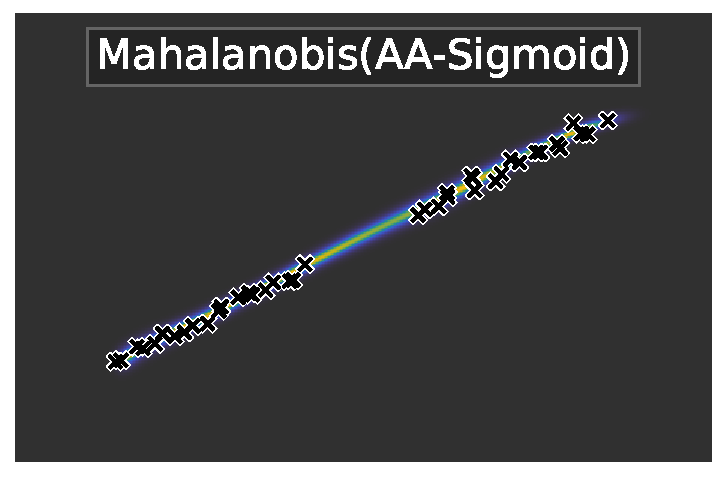
\includegraphics[width=0.388\textwidth,valign=t]{ood-detection/figures/ood-detection/confidence-line-aa-sigmoid-mahalanobis.pdf}
    \end{subfigure}
    \begin{subfigure}
        \centering
        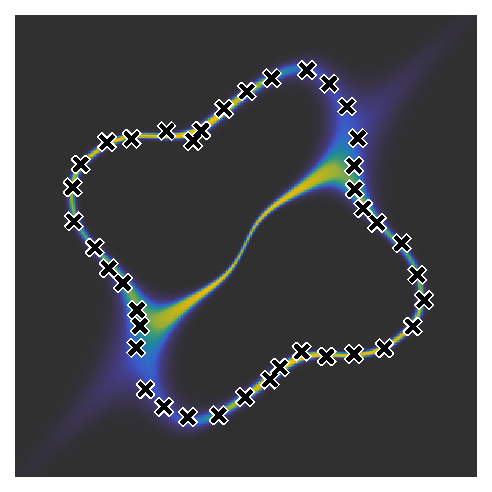
\includegraphics[width=0.254\textwidth,valign=t]{ood-detection/figures/ood-detection/confidence-circle-aa-sigmoid-mahalanobis.pdf}
    \end{subfigure}
    \begin{subfigure}
        \centering
        \includegraphics[width=0.308\textwidth,valign=t]{ood-detection/figures/ood-detection/confidence-haystack-aa-sigmoid-mahalanobis.pdf}
    \end{subfigure}

    \caption[Comparison of Mahalanobis-transformed Auto-Associative Networks as OOD detection methods]{By-example (see \Cref{txt:ood-detection-comparison}) evaluation of Auto-Associative networks (see \Cref{txt:auto-associative}) as OOD detection methods. The networks use the ReLU or sigmoid activation function, and their per-feature reconstruction errors are transformed into a confidence score via the Mahalanobis distance (see \Cref{eq:mahalanobis-distance}).}
    \label{fig:auto-associative-mahalanobis-ood-detection}
\end{figure}

\noindent The bad fits generated by the ReLU activation function for the line example and the sigmoid activation function for the circular case motivate the exploration of Gaussian Processes (GPs, see \Cref{txt:gaussian-process}) as an auto-associative predictor. While using GPs as an uncertainty-based method for OOD detection is discussed in \Cref{txt:ood-detection-analysis-uq}, here they are fit on the input $X$ to predict $X$ such that the auto-associative prediction uncertainty and error can be measured. \Cref{fig:auto-associative-gp-ood-detection} highlights two possible approaches.

\begin{figure}[H]
    \centering
    \begin{subfigure}
        \centering
        \includegraphics[width=0.388\textwidth,valign=t]{ood-detection/figures/ood-detection/confidence-line-gp-coarse-xx.pdf}
    \end{subfigure}
    \begin{subfigure}
        \centering
        \includegraphics[width=0.254\textwidth,valign=t]{ood-detection/figures/ood-detection/confidence-circle-gp-coarse-xx.pdf}
    \end{subfigure}
    \begin{subfigure}
        \centering
        \includegraphics[width=0.308\textwidth,valign=t]{ood-detection/figures/ood-detection/confidence-haystack-gp-coarse-xx.pdf}
    \end{subfigure}

    \begin{subfigure}
        \centering
        \includegraphics[width=0.388\textwidth,valign=t]{ood-detection/figures/ood-detection/confidence-line-gp-xx-mahalanobis.pdf}
    \end{subfigure}
    \begin{subfigure}
        \centering
        \includegraphics[width=0.254\textwidth,valign=t]{ood-detection/figures/ood-detection/confidence-circle-gp-xx-mahalanobis.pdf}
    \end{subfigure}
    \begin{subfigure}
        \centering
        \includegraphics[width=0.308\textwidth,valign=t]{ood-detection/figures/ood-detection/confidence-haystack-gp-xx-mahalanobis.pdf}
    \end{subfigure}

    \caption[Comparison of Auto-Associative Gaussian Processes as OOD detection methods]{By-example (see \Cref{txt:ood-detection-comparison}) evaluation of Auto-Associative (see \Cref{txt:auto-associative}) Gaussian Processes (see \Cref{txt:gaussian-process}), optionally using the Mahalanobis distance (see \Cref{eq:mahalanobis-distance}), as OOD detection methods.}
    \label{fig:auto-associative-gp-ood-detection}
\end{figure}

\noindent In the first approach, the auto-associative GP predicts per-feature-uncertainties, which are summed up and transformed into an OOD confidence score. This method works remarkably well on all three examples, even when trained on just $1\%$ of the available training data. In the line example, a 1D ID-input subspace may be preferable, such as the one the truncated PCA method extracts in \Cref{fig:truncated-pca-ood-detection}. However, producing high confidence around the training points and allowing some lower-confidence interpolation in between also provides valuable OOD detection. Furthermore, this method generates similarly tight confidence spikes as the auto-associative networks using the Mahalanobis distance.

The second approach compares the auto-associative GP's mean predictions with the original input. The per-feature errors, which are summed or transformed with the Mahalanobis distance, produce the confidence score. Unfortunately, while this method generates an even thinner spike in the haystack example, it also produces artefacts in the line and circle examples, both with and without the Mahalanobis distance.

\subsection{Surprisingly Successful Uncertainty-based Methods} \label{txt:ood-detection-analysis-uq}

\begin{figure}[H]
    \centering
    \begin{subfigure}
        \centering
        \includegraphics[width=0.388\textwidth,valign=t]{ood-detection/figures/ood-detection/confidence-line-rf.pdf}
    \end{subfigure}
    \begin{subfigure}
        \centering
        \includegraphics[width=0.254\textwidth,valign=t]{ood-detection/figures/ood-detection/confidence-circle-rf.pdf}
    \end{subfigure}
    \begin{subfigure}
        \centering
        \includegraphics[width=0.308\textwidth,valign=t]{ood-detection/figures/ood-detection/confidence-haystack-rf.pdf}
    \end{subfigure}

    \caption[Random Forest Uncertainty for OOD Detection]{By-example (see \Cref{txt:ood-detection-comparison}) evaluation of using Random Forest (see \Cref{txt:ensembles-decision-tree-random-forest}) ensemble prediction variation for OOD detection.}
    \label{fig:uq-rf-ood-detection}
\end{figure}

Model uncertainty and confidence are not equivalent. While the former describes the expected prediction error, the latter determines whether a prediction of the target value and its uncertainty can be used at all. Therefore, OOD uncertainty estimates are only valuable if the model is constructed and trained to have high uncertainty on inputs that deviate from the ID training data. If this is the case, it can be convenient to use unexpectedly high prediction uncertainty as a proxy for low confidence. In this subsection, we evaluate two uncertainty-based methods for OOD detection. In each, a model is trained on the ID input-output pairs, and its prediction uncertainty on unseen data is translated into a confidence score.

Random Forests (RFs) (see \Cref{txt:ensembles-decision-tree-random-forest}) are a generalist method that utilises bootstrapping to produce high-quality predictions even in higher dimensions and without hyperparameter-tuning \cite{ml-hyperparameters-2021}. However, RFs are also prone to overgeneralising where possible. For example, \Cref{fig:uq-rf-ood-detection} shows that the high-confidence areas extracted by analysing the variance across the forest's predictions have outgoing streaks that reach infinitely far into the OOD space. RFs also fail to find any difference between ID and OOD inputs in the haystack task.

\begin{figure}[H]
    \centering
    \begin{subfigure}
        \centering
        \includegraphics[width=0.388\textwidth,valign=t]{ood-detection/figures/ood-detection/confidence-line-gp-coarse-xy.pdf}
    \end{subfigure}
    \begin{subfigure}
        \centering
        \includegraphics[width=0.254\textwidth,valign=t]{ood-detection/figures/ood-detection/confidence-circle-gp-coarse-xy.pdf}
    \end{subfigure}
    \begin{subfigure}
        \centering
        \includegraphics[width=0.308\textwidth,valign=t]{ood-detection/figures/ood-detection/confidence-haystack-gp-coarse-xy.pdf}
    \end{subfigure}

    \begin{subfigure}
        \centering
        \includegraphics[width=0.388\textwidth,valign=t]{ood-detection/figures/ood-detection/confidence-line-gp.pdf}
    \end{subfigure}
    \begin{subfigure}
        \centering
        \includegraphics[width=0.254\textwidth,valign=t]{ood-detection/figures/ood-detection/confidence-circle-gp.pdf}
    \end{subfigure}
    \begin{subfigure}
        \centering
        \includegraphics[width=0.308\textwidth,valign=t]{ood-detection/figures/ood-detection/confidence-haystack-gp.pdf}
    \end{subfigure}

    \caption[Gaussian Process uncertainty for OOD detection]{By-example (see \Cref{txt:ood-detection-comparison}) evaluation of Gaussian Processes (see \Cref{txt:gaussian-process}) with different training data subsample sizes as OOD detection methods.}
    \label{fig:uq-gp-ood-detection}
\end{figure}

\noindent Gaussian Processes (see \Cref{txt:gaussian-process}) are a stochastic method to smoothly fit a function to a given set of training points \cite{gp-ml-2005}. Given their high computational complexity, $\text{O}(N^3)$ for $N$ data points, fitting them is expensive and often only possible using approximation or a subset of the data. \Cref{fig:uq-gp-ood-detection} shows that while a GP trained on just $1\%$ of the data already performs very well in the line and circle cases, it only produces a very gradual drop in confidence for the haystack. At $10\%$ of the data and 1000-times the computational cost, the GP shows a much better confidence peak similar to the ones produced by auto-associative methods in \Cref{txt:ood-detection-analyis-auto-associative}.

\subsection{Challenges with Noise-Contrastive Priors} \label{txt:ood-detection-analysis-ncp}

\Cref{txt:uq-conf-method} summarises how \textcite{noise-contrastive-uq-2020} use noise-contrastive priors to train a probabilistic model to have high uncertainty for OOD inputs. Inspired by their work, we also test whether training the uncertainty-based OOD detectors with probably-OOD perturbed input-output pairs alongside the ID points improves their OOD detection. \Cref{fig:ncp-gp-rf-ood-detection} shows that their effectiveness varies.

For Gaussian Processes, they smudge the high-confidence areas to span more OOD inputs since they now contain \textit{some} training samples. While no effect on the circular example can be observed, the noise-contrastive GPs fail entirely for the haystack, even though standard GPs handle that case well. This failure highlights that inventing OOD inputs for training may confuse sensitive models such as Gaussian processes. \Cref{txt:ood-synthesis-analysis} explores different strategies for training with synthetic OOD samples.

For Random Forests, however, the noise-contrastive method provides a clear improvement. Training them with high-uncertainty noise-perturbed inputs alongside the OOD data forces the RFs to learn a tight boundary around the ID inputs, removing the over-generalising high-confidence streaks seen in \Cref{fig:uq-rf-ood-detection}, and thus bringing their performance almost on par with the Local Outlier Factor (see \Cref{fig:md-lof-ood-detection}). Note, however, that the confidence maps produced by the RF also contain widespread subtle noise artefacts, and that the RF still fails to succinctly identify OOD inputs in the haystack example.

\begin{figure}[H]
    \centering
    \begin{subfigure}
        \centering
        \includegraphics[width=0.388\textwidth,valign=t]{ood-detection/figures/ood-detection/confidence-line-nc-gp.pdf}
    \end{subfigure}
    \begin{subfigure}
        \centering
        \includegraphics[width=0.254\textwidth,valign=t]{ood-detection/figures/ood-detection/confidence-circle-nc-gp.pdf}
    \end{subfigure}
    \begin{subfigure}
        \centering
        \includegraphics[width=0.308\textwidth,valign=t]{ood-detection/figures/ood-detection/confidence-haystack-nc-gp.pdf}
    \end{subfigure}

    \begin{subfigure}
        \centering
        \includegraphics[width=0.388\textwidth,valign=t]{ood-detection/figures/ood-detection/confidence-line-nc-rf.pdf}
    \end{subfigure}
    \begin{subfigure}
        \centering
        \includegraphics[width=0.254\textwidth,valign=t]{ood-detection/figures/ood-detection/confidence-circle-nc-rf.pdf}
    \end{subfigure}
    \begin{subfigure}
        \centering
        \includegraphics[width=0.308\textwidth,valign=t]{ood-detection/figures/ood-detection/confidence-haystack-nc-rf.pdf}
    \end{subfigure}

    \caption[Noise-Contrastive Priors for OOD detection]{By-example (see \Cref{txt:ood-detection-comparison}) evaluation of Noise-Contrastive Priors (see \Cref{txt:uq-conf-method}) for Gaussian Processes (see \Cref{txt:gaussian-process}) and Random Forests (see \Cref{txt:ensembles-decision-tree-random-forest}) as OOD detection methods.}
    \label{fig:ncp-gp-rf-ood-detection}
\end{figure}

\subsection{Recommendations for OOD Detection Methods} \label{txt:ood-detection-summary}

This section has visually evaluated several OOD detection methods based on three simple and intuitive test cases. We have developed these three toy examples to catch potential OOD detection failure cases early -- if a method does not work in these 2D examples, how can we trust it to work on high-dimensional data where it is much more challenging to define what non-trivial OOD inputs look like?

\newpar From these experiments, we can provide the following recommendations:
\begin{enumerate}
    \item If the dimensionality is low, ID samples are uniformly spread within the ID subspace, and conceptual generalisation to unseen data is not as important, the Local Outlier Factor provides a very simple yet effective method.
    \item If conceptual generalisation is desired, auto-associative networks provide an intuitive method for identifying the ID subspace. However, these neural networks require additional tuning to reduce the confidence map artefacts generated from suboptimal training. Applying the Mahalanobis distance to the reconstruction errors generally improves the confidence map quality. If the ID subspace is linear, truncated PCA provides a cheaper implementation than neural networks.
    \item Gaussian Process uncertainty performs surprisingly well across all examples at detecting OOD. However, their computational cost and decreased performance in higher dimensions limit their applicability.
\end{enumerate}

\noindent In this work, we focus on fitting a response surface model for the SOSAA simulation. Thus, conceptual generalisation is desirable, and we choose to explore auto-associative networks for OOD detection further.

\section{Toy-Comparisons of OOD Synthesis Methods} \label{txt:ood-synthesis-analysis}

\Cref{txt:ood-detection-comparison} has analysed the performance of different OOD detection methods using three toy examples. Most of these methods, excluding noise-contrastive priors, only use ID inputs to train their detectors since often no OOD samples are available. However, tasks such as providing meaningful OOD confidence scores, which \Cref{txt:confidence-scoring-comparison} explores, benefit from being trained with both ID and OOD samples \cite{ood-exposure-2018}. Specifically, examples of OOD inputs provide tangible signals during training as to where to strike the balance between which inputs should be accepted as ID with high confidence and for which the model should be weary. Having OOD samples thus makes it easier to integrate OOD detection with other tasks in a joint model loss function.

However, training with OOD samples requires actually having access to OOD samples. While OOD datasets exist for some tasks, such as image recognition, synthesising OOD inputs is a more flexible and powerful approach. \Cref{txt:ood-input-generation} provides an overview of the Boundary Aware Learning method \cite{ood-boundary-2021}, which serves as inspiration for the techniques explored in this section.

\newpar As in the previous section, the comparison figures are split into three columns that highlight each method's performance across three toy examples: (1)st two groups of points on a line, (2)nd points on the boundary of a sine-perturbed circle, and (3)rd a 10-dimensional multivariate normal distribution in which one feature is constant. Please refer to \Cref{txt:ood-detection-comparison} for a more detailed introduction to these toy examples. Given the ID input points for each toy example, each method is tasked with generating synthetic OOD inputs. Next, a multi-layer classifier is trained on both the ID and synthetic OOD inputs using the default settings in the \texttt{scikit-learn} library \cite{scikit-learn-2011}. Specifically, the network has one layer with 100 neurons using the ReLU activation function, which provides a level playing ground for all tested methods. This classifier's predicted probability that an input is in-distribution is then used as the ID confidence value. Each plot shows the predicted confidence for points surrounding the ID inputs using the CET-L20 colour map \cite{color-cet-2015, color-cet-2023} from black for OOD over blue and green to yellow for ID points. A subsample of the ID inputs is shown as black \texttt{x} markers, and some of the synthetic OOD inputs are shown as white dots. The haystack example plots are again adapted for their high dimensionality and only show the distribution of ID confidence values on the y-axis for different inputs for the constant feature on the x-axis. The location of the constant seen in training is highlighted as a white line. Since the confidence detection model is the same across all methods, these figures only evaluate the effect that the OOD synthesis has on the performance of the detector. Ideally, the detector should be highly confident in ID inputs, classify most of the input feature space as OOD, and produce a tight and sharp boundary around the ID manifold.

\subsection{Trivial Random OOD Inputs as a Baseline} \label{txt:uniform-ood-synthesis-analysis}

The most trivial technique for generating synthetic OOD inputs is to sample random noise, which is used in many methods \cite[e.g.][]{ood-class-2022, ood-boundary-2021, ood-training-2017, ood-exposure-confidence-2021, learning-ood-confidence-2018, noise-contrastive-uq-2020}. While normal-distributed samples, drawn independently per feature, may provide the desired coverage of the input space for some input domains, we follow \textcite{ood-boundary-2021} and use uniformly distributed random inputs but widen their range slightly beyond the training data. While we could also generate random output labels and train a detector on the increased uncertainty for OOD inputs as \textcite{noise-contrastive-uq-2020} propose, \Cref{txt:uq-conf-method} and \Cref{txt:ood-detection-analysis-ncp} have already explored this approach and its flaws. To avoid having to assume a fixed output range, we only generate synthetic OOD inputs.

\begin{figure}[H]
    \centering
    \begin{subfigure}
        \centering
        \includegraphics[width=0.388\textwidth,valign=t]{ood-detection/figures/ood-synthesis/ood-line-uniform.pdf}
    \end{subfigure}
    \begin{subfigure}
        \centering
        \includegraphics[width=0.254\textwidth,valign=t]{ood-detection/figures/ood-synthesis/ood-circle-uniform.pdf}
    \end{subfigure}
    \begin{subfigure}
        \centering
        \includegraphics[width=0.308\textwidth,valign=t]{ood-detection/figures/ood-synthesis/ood-haystack-uniform.pdf}
    \end{subfigure}

    \caption[Random Synthetic OOD Samples]{By-example (see \Cref{txt:ood-synthesis-analysis}) evaluation of uniformly sampling OOD inputs.}
    \label{fig:uniform-ood-samples}
\end{figure}

\noindent \Cref{fig:uniform-ood-samples} shows that just by sampling OOD inputs uniformly, the OOD detector already learns reasonable boundaries for the line and circle examples. Note that in the line example, the extracted ID subspace is cut off since no ID samples are present in the lower left corner, and the ReLU activation function used in the neural network OOD detector is prone to cutting off some of the input space if possible. In the circle toy example, this simple method produces a box-like outline that roughly fits the circle boundary. Note, however, that the detector is never fully confident, even very close to the ID inputs, since many uniformly sampled OOD inputs overlap with the ID space. Unfortunately, uniformly sampling OOD inputs fails entirely on the haystack example as the OOD detector is unable to identify any OOD inputs and instead classifies all inputs as ID.

\subsection{Adversarial OOD Inputs using the Fast Gradient Sign Method} \label{txt:adversarial-ood-synthesis-analysis}

Adversarial methods provide a more targeted approach to generating OOD inputs. In the following experiments, we test the cheap Fast Gradient Sign Method (FGSM) \cite{fast-gradient-2014}. Given some input $x$ and a predictor $f(x)$, it finds a small perturbation that significantly increases the prediction error $E(x)$:
\begin{equation*}
    x' = x + \epsilon \cdot \text{sign} \left( \frac{\partial E(x)}{\partial x} \right)
\end{equation*}
where $\epsilon$ is the perturbation step length and $E(x)$ is some prediction error function. Given the success of auto-associative networks in learning the ID input subspace in \Cref{txt:ood-detection-analyis-auto-associative}, we reuse them here to provide reconstruction error gradients. For these experiments, we manually implement a `perfect' auto-associative mapping. Thus, only the FGSM method, but not its source of gradients, is evaluated. For instance, the perfect auto-associative mappings for the line and circle toy examples reconstruct an input point by projecting it onto the exact line and circle boundary from which the ID points were sampled with noise. In the haystack example, the reconstruction simply resets the constant-in-training feature to the constant value seen during training. It is also worth noting that the FGSM method is not directly applied to the ID training points but to a random sample of points generated from a Gaussian kernel density estimation of the ID training data (see \Cref{txt:online-distribution-fitting}).

The first row in \Cref{fig:fgsm-t-poking-ood-samples} shows that the FGSM method with a constant perturbation step size of $\epsilon = 1$ succeeds at synthesising OOD samples that suggest a clear boundary to the OOD input space. The extracted high-confidence areas are promising, and the OOD detector is highly confident in both ID and OOD classifications. However, the boundaries could be tighter, which is especially apparent in the haystack example.

\newpar Why does the FGSM in the line example only produce OOD points that are parallel to the ID line but none in the middle of the two groups of points? In these examples, the gradients for the FGSM come from the reconstruction error of a `perfect' auto-associative mapping which matches our interpretation of an ideal OOD detector that was introduced in \Cref{fig:ideal-ood-detection}. While assigning the space between the two groups as OOD would be a valid interpretation, we are particularly interested in our experiments in methods that can extract the assumption subspace of the ID inputs instead of relying on input density alone.

\begin{figure}[H]
    \centering
    \begin{subfigure}
        \centering
        \includegraphics[width=0.388\textwidth,valign=t]{ood-detection/figures/ood-synthesis/ood-line-fgsm.pdf}
    \end{subfigure}
    \begin{subfigure}
        \centering
        \includegraphics[width=0.254\textwidth,valign=t]{ood-detection/figures/ood-synthesis/ood-circle-fgsm.pdf}
    \end{subfigure}
    \begin{subfigure}
        \centering
        \includegraphics[width=0.308\textwidth,valign=t]{ood-detection/figures/ood-synthesis/ood-haystack-fgsm.pdf}
    \end{subfigure}

    \begin{subfigure}
        \centering
        \includegraphics[width=0.388\textwidth,valign=t]{ood-detection/figures/ood-synthesis/ood-line-poking-fgsm.pdf}
    \end{subfigure}
    \begin{subfigure}
        \centering
        \includegraphics[width=0.254\textwidth,valign=t]{ood-detection/figures/ood-synthesis/ood-circle-poking-fgsm.pdf}
    \end{subfigure}
    \begin{subfigure}
        \centering
        \includegraphics[width=0.308\textwidth,valign=t]{ood-detection/figures/ood-synthesis/ood-haystack-poking-fgsm.pdf}
    \end{subfigure}

    \caption[Adversarial Synthetic OOD Samples and $t$-poking]{By-example (see \Cref{txt:ood-synthesis-analysis}) evaluation of adversarially sampling OOD inputs using the Fast Gradient Sign Method \cite{fast-gradient-2014}. While the variant in the first row fixes the gradient step size to $\epsilon = 1$, $t$-poking is used to optimise the constant $\epsilon = t_{poke}$ in the second row.}
    \label{fig:fgsm-t-poking-ood-samples}
\end{figure}

\noindent Several approaches can produce tighter OOD detection bounds around the ID manifold. While it is possible to tweak the step size manually, this is a cumbersome process. The tweaking can instead be automated with a simple method that we call $t$-poking. This approach sets the step size to a new parameter $t$ or a small distribution of values surrounding $t$. After every batch or epoch, the performance of the OOD detector is evaluated on the ID training inputs (and optionally on the FGSM-synthesised OOD inputs) using success criteria such as ``the mean confidence score for ID inputs should not fall below $0.95$''. If the current detector does not meet these criteria, $t$ is multiplied by a back-off factor $>1$. Conversely, if the detector meets the criteria, $t$ is multiplied by a poking factor $<1$. Thus, a balanced $t$ is automatically determined based on a set of easily interpretable criteria for the OOD detector. Suppose this strategy is applied whilst the detector is being trained. In that case, the $t$ value is continuously updated and decreased by poking the detector to see if it has already improved enough to learn an even tighter boundary.

The second row in \Cref{fig:fgsm-t-poking-ood-samples} shows that $t$-poking is indeed able to push the OOD samples very close to the ID boundary. In particular, it finds $t_{poke} = 0.172$, $t_{poke} = 0.451$, and $t_{poke} \approx 0.0183$ for these specific line, circle, and haystack experiments. Identifying the $t_{poke}$ value is more difficult in the haystack example as the OOD detector's performance is flaky for low step sizes in our experiments. Nevertheless, $t$-poking is able to extract a very tight needle boundary in the haystack example.

\begin{figure}[H]
    \centering
    \begin{subfigure}
        \centering
        \includegraphics[width=0.388\textwidth,valign=t]{ood-detection/figures/ood-synthesis/ood-line-uniform-fgsm.pdf}
    \end{subfigure}
    \begin{subfigure}
        \centering
        \includegraphics[width=0.254\textwidth,valign=t]{ood-detection/figures/ood-synthesis/ood-circle-uniform-fgsm.pdf}
    \end{subfigure}
    \begin{subfigure}
        \centering
        \includegraphics[width=0.308\textwidth,valign=t]{ood-detection/figures/ood-synthesis/ood-haystack-uniform-fgsm.pdf}
    \end{subfigure}

    \caption[Adversarially Uniform Synthetic OOD Samples]{By-example (see \Cref{txt:ood-synthesis-analysis}) evaluation of adversarially sampling OOD inputs using the Fast Gradient Sign Method \cite{fast-gradient-2014} where the gradient step size is sampled from the standard uniform distribution.}
    \label{fig:fgsm-uniform-ood-samples}
\end{figure}

\noindent Another approach for producing tighter boundaries is to draw the gradient step size from a distribution, as recommended by \textcite{ood-boundary-2021}. While they sample from the normal distribution, we use the standard uniform distribution, as shown in \Cref{fig:fgsm-uniform-ood-samples}. This simple approach works quite well. Using the FGSM method improves upon the purely uniform OOD samples in \Cref{fig:uniform-ood-samples} by providing more targeted OOD points that better constrain the ID-OOD boundary. For instance, the ID subspace in the line example now extends further in both directions, though it gets slightly narrower towards the bottom left corner. Furthermore, the ID needle is now identified in the haystack example. However, as the circle example highlights, this simple method can also easily fail. Here, the confidence for many of the ID training points in the circle example suffers due to the overlap between ID and OOD inputs. Furthermore, some confidence smidges extend the high-confidence areas into clearly OOD areas. How could these issues caused by the overlap of ID and OOD inputs be avoided?

\subsection{A brief Introduction to Weighting ID vs OOD Samples} \label{txt:id-ood-weighting}

How can the overlap between ID and synthetic OOD points be handled during training? If we have a very high-dimensional feature space and a small ID subspace, it may be sufficient to generate OOD samples. \textcite{ood-training-2017} present just one of the methods described in \Cref{txt:ood-input-generation} that use adversarial algorithms to generate OOD samples that are much closer to the ID boundary, which not only improves the detector's decision boundary but also seemingly circumvents the problem of a clash between OOD and ID samples. However, as the ID manifold expands to cover close to or all of the input feature space, it becomes increasingly challenging even for these methods to generate OOD samples that do not overlap the ID manifold. This potential failure case motivates adding a weighting factor to ID and OOD samples.

\newpar We first define the problem as finding a weighting function $w_{\text{OOD}}(X) \in [0.0; 1.0]$ that maps an input $X$ to a sample weight factor. OOD inputs outside the ID manifold should be given full weight. In contrast, OOD inputs that clash with ID inputs should be given a lower sampling weight. The weighting is motivated as follows:

We assume that there is a distribution $\mathbb{P}_{X}$ of semantically valid input features that is a superset of the ID and OOD distributions. An OOD detector is ideally trained on samples from the entirety of $\mathbb{P}_{X}$. However, in reality, it is only trained on the ID training samples and some synthetically generated OOD inputs. Since the latter may contain some misclassified ID inputs, we want to prioritise ID samples over synthetic OOD samples. Thus, after the ID inputs have been drawn from $\mathbb{P}_{X}$, they partially block off parts of the distribution. When synthetic OOD inputs are then generated, samples that fall within ID areas are blocked and weighted down. \Cref{fig:id-ood-weights} uses a simple example to walk through how we design the OOD sample weight factor $\textcolor{matplotlib-4}{w_{\text{OOD}}(X)}$:

\begin{multicols}{2}
    \noindent For our weighting scheme, we first need to calculate the probability density functions (pdf) of the \textcolor{confidence-any}{input domain distribution $\mathbb{P}_X$}, the \textcolor{confidence-id}{in-distribution $\mathbb{P}_{X_{\text{ID}}}$} and the \textcolor{confidence-ood}{out-of-distribution $\mathbb{P}_{X_{\text{OOD}}}$}. Since we may not know the analytical form for all of them, in particular for the \textcolor{confidence-id}{in-distribution}, we can instead approximate the pdf using sampling-based methods, as shown in the first plot of \Cref{fig:id-ood-weights}. \Cref{txt:online-distribution-fitting} describes how distribution fitting can be used to approximate the pdfs, e.g. online inside a neural network's training loop. In higher-dimensional domains, choosing a lower-dimensional proxy may also be beneficial as its pdf can be better approximated with a limited number of samples. For instance, the 1D distribution of the reconstruction error $E(X)$ of an auto-associative network (see \Cref{txt:auto-associative}) can be used as a proxy:
    \begin{equation*}
        \textcolor{confidence-id}{P_{q}(X)} \approx P(E(X) \given X \in \mathbb{P}_{q}) \text{ where } q \in \{ X, \text{ID}, \text{OOD} \}
    \end{equation*}

    \noindent Remember that the \textcolor{confidence-id}{ID} and the \textcolor{confidence-ood}{OOD} samples both come from \textcolor{confidence-any}{input domain distribution} but have likely sampled it with bias. To make apparent which areas of the \textcolor{confidence-any}{input domain} have already been sampled, we rescale all three pdfs such that the \textcolor{confidence-any}{input data pdf} dominates both the \textcolor{confidence-id}{\text{ID}} and \textcolor{confidence-ood}{\text{OOD}} pdfs, i.e. $\forall X \st \textcolor{confidence-id}{f_{\text{ID}}(X)} \leq \textcolor{confidence-any}{f_{X}(X)}$ and $\forall X \st \textcolor{confidence-ood}{f_{\text{OOD}}(X)} \leq \textcolor{confidence-any}{f_{X}(X)}$, both are equal to $\textcolor{confidence-any}{f_{X}(x)}$ for some $\textcolor{confidence-any}{x \in X}$, and $\max(\textcolor{confidence-any}{f_{X}}) = 1.0$. We can now see in the second plot which areas of the \textcolor{confidence-any}{input domain} have already been sampled and how frequently.

    Note that some of the areas have been sampled twice, i.e. the \textcolor{confidence-id}{ID pdf} and the \textcolor{confidence-ood}{OOD pdf} overlap. In our motivation above, we have stated that we want to prioritise \textcolor{confidence-id}{ID} samples over \textcolor{confidence-ood}{OOD} samples, in effect blocking conflicting \textcolor{confidence-ood}{OOD} samples. Thus, to only count \textcolor{confidence-id}{ID samples} and \textcolor{confidence-ood}{OOD samples} that do not conflict with them, we ignore the area below the \textcolor{confidence-ood}{OOD pdf curve} wherever it overlaps with the area below the \textcolor{confidence-id}{ID pdf}.

    Finally, we can calculate the weighting factor for \textcolor{confidence-id}{ID} and \textcolor{confidence-ood}{OOD} samples. For any input \textcolor{confidence-any}{$x \in X$}, we look at the fraction of the area under the combined sampling curves, $\text{max}(\textcolor{confidence-id}{f_{\text{ID}}(X)}, \textcolor{confidence-ood}{f_{\text{OOD}}(X)})$, that is taken up by \textcolor{confidence-id}{ID} to calculate the ID sample weight. The OOD sample weight $\textcolor{matplotlib-4}{w_{\text{OOD}}(X)}$ is simply its complement:
    \begin{equation} \label{eq:ood-weight}
        \textcolor{matplotlib-4}{w_{\text{OOD}}(X)} = 1 - \frac{\textcolor{confidence-id}{f_{\text{ID}}(X)}}{\max(\textcolor{confidence-id}{f_{\text{ID}}(X)}, \textcolor{confidence-ood}{f_{\text{OOD}}(X)})}
    \end{equation}

    \noindent This scheme ensures that areas of the \textcolor{confidence-any}{input domain} that the \textcolor{confidence-id}{ID samples} dominate, shown as a \textcolor{confidence-id}{striped-yellow} area in \Cref{fig:id-ood-weights}, are assigned zero \textcolor{matplotlib-4}{OOD weight} such that \textcolor{confidence-id}{ID} and \textcolor{confidence-ood}{OOD} samples no longer overlap there. Regions without ID inputs, shown in \textcolor{confidence-ood}{striped-dark-blue}, are assigned full \textcolor{matplotlib-4}{OOD weight}. Notably, if $\textcolor{confidence-id}{X_{\text{ID}}}$ expands to cover all of $\textcolor{confidence-any}{X}$, the \textcolor{matplotlib-4}{OOD weight} is $0$ for all inputs, \textit{regardless} of the \textcolor{confidence-ood}{OOD sampling}.

    \begin{figure}[H]
        \centering
        \begin{subfigure}
            \centering
            \includegraphics[width=0.49\textwidth]{ood-detection/figures/weighting/id-ood-weights-1.pdf}
        \end{subfigure}

        \vspace{-1em}
        \begin{subfigure}
            \centering
            \includegraphics[width=0.49\textwidth]{ood-detection/figures/weighting/id-ood-weights-2.pdf}
        \end{subfigure}

        \vspace{-1em}
        \begin{subfigure}
            \centering
            \includegraphics[width=0.49\textwidth]{ood-detection/figures/weighting/id-ood-weights-3.pdf}
        \end{subfigure}

        \vspace{-2em}
        \caption[ID-OOD Weighting Example]{Example of the ID-OOD sample weighting scheme. The \textcolor{confidence-any}{input space} covers $\textcolor{confidence-any}{X} \in [-6; 6]$ and is uniformly sampled. The \textcolor{confidence-id}{ID distribution} follows $\textcolor{confidence-id}{X_{\text{ID}}} \sim \sum_{i=1}^{12}\left(\text{U}(0, 1)\right) - 6$, an Irwin-Hall distribution. The \textcolor{confidence-ood}{synthetic OOD samples} come from a mirrored triangular distribution that overlaps with ID samples.}
        \label{fig:id-ood-weights}
    \end{figure}
\end{multicols}

\noindent It is worth noting that the weighting function in \Cref{eq:ood-weight} imposes a definition of the ID vs OOD boundary onto the OOD detector. Specifically, it filters out any OOD samples within the ID manifold's high-density regions, ensuring that the detector confidently predicts ID inputs inside them. While this has little impact on sparse feature spaces, it protects the detector from confusion as the in-distribution manifold expands to fill the entire input space. In \Cref{txt:weighted-ood-synthesis-analysis}, we investigate if the OOD down-weighting benefits any method using uniformly or normally sampled OOD inputs, particularly the ones discussed in \Cref{txt:uniform-ood-synthesis-analysis} and \Cref{txt:adversarial-ood-synthesis-analysis}, which are vulnerable to false detector confusion through clashes between synthetic OOD and real ID inputs.

\subsection{On-the-fly OOD vs ID Sample Weighting using Distribution Fitting} \label{txt:online-distribution-fitting}

The OOD sample weighting described in \Cref{txt:id-ood-weighting} relies on calculating the probability density functions of the input domain distribution $\mathbb{P}_X$, the in-distribution $\mathbb{P}_{X_{\text{ID}}}$ and the out-of-distribution $\mathbb{P}_{X_{\text{OOD}}}$. When the analytical form of these pdfs is not known, they can be approximated using distribution fitting. This section briefly explores different distribution fitting methods and how they can be used online on the fly.

\newpar First, we must choose which distribution to fit. Problem-domain-specific knowledge can often be used to identify a parametric distribution that fits the sample data well. For instance, a well-trained neural network following the classical linear regression model is assumed to produce normal-distributed prediction errors with zero mean \cite{clrm-assuptions-1971}. In this case, the normal distribution $\text{N}(0, \sigma^2)$ can be fit by measuring the standard deviation $\sigma$. However, in more complex cases, the distribution shape may be unknown or shift over time, e.g. if the OOD sample weighting is employed in a continuous learning process where the machine learning model continuously receives new training data \cite{lifelong-learning-2017}. Kernel Density Estimation (KDE) is one non-parametric method to estimate the probability density given some independently and identically distributed (iid) samples \cite{kde-1956, kde-1962}. Given a set of training data $X = \{x_1, x_2, ..., x_{N} \}$ and a positive kernel bandwidth parameter $h$, the density for a new data point $x$ is computed as follows:
\begin{equation} \label{eq:kernel-density}
    f(x) = \frac{1}{N \cdot h} \sum_{i = 1}^{N} K \left( \frac{x - x_i}{h} \right)
\end{equation}
where $K$ is a non-negative kernel function, e.g. the pdf of the standard normal distribution. While KDE generalises well to higher dimensions, a simpler approach can be taken for a one-dimensional distribution, such as the sum reconstruction error of an auto-associative network. If some quantiles of a distribution are known, \textcite{pdf-quantiles-2018} suggests fitting the integral of a cubic B-spline with non-negative coefficients to the quantiles, such that the spline smoothly approximates the distribution's pdf.

\newpar If the data distributions are fixed or only need to be refitted infrequently, more complicated distribution fitting procedures can be performed on a large sample of data before any OOD sample reweighting occurs. However, suppose the model is instead trained continuously on a stream of incoming data where the ID and OOD distributions can shift over time, e.g. when the OOD inputs come from a jointly trained adversarial generator. In that case, the distribution fitting must be performed online. KDE can be applied online if some window of the most recent points is kept in memory and evaluated for every new point. Quantile-based distribution fitting methods, including \citeauthor{pdf-quantiles-2018}'s spline and parametric methods, can also be applied by using online quantile regression algorithms to keep a running estimate of the quantiles \cite{p2-quantile-1985, frugal-quantiles-2014, quantile-outlier-2020}. \textcite{online-median-2021} presents a remarkably concise running quantile estimator that generalises the running median algorithm introduced by \textcite{median-perceptron-1997}:
\begin{equation*}
    Q_{k+1} = Q_k + \epsilon \cdot (\text{sign}(x_{k+1} - Q_k) + 2 \cdot p - 1) \quad \text{where } Q_1 = 0
\end{equation*}
where $Q_{k+1}$ is the estimate of the $(100 \cdot p) \%$-quantile of the observed samples up to $x_{k+1}$ at time step $k+1$, which is updated every time step by a small positive step size $\epsilon$. The simplicity of this estimator makes it well-suited for continuously estimating many quantiles inside a neural network training loop in order to produce a precise fit for the $\mathbb{P}_X$, $\mathbb{P}_{X_{\text{ID}}}$ and $\mathbb{P}_{X_{\text{OOD}}}$ distributions that are required by the OOD weighting scheme.

\subsection{Evaluation of OOD-Weighting with Uniform and Adversarial Samples} \label{txt:weighted-ood-synthesis-analysis}

This section evaluates the impact of applying the OOD vs ID sample weighting scheme introduced in \Cref{txt:id-ood-weighting} to both the uniform and FGSM-based OOD synthesis approaches. Since the OOD samples are in both cases sampled using some uniform sampling, we assume for implementation simplicity that $\mathbb{P}_X = \mathbb{P}_{X_{\text{OOD}}}$. The two following comparison plots come in pairs to better visualise the differences in confidence prediction that the weighting produces.

\begin{figure}[H]
    \centering
    \begin{subfigure}
        \centering
        \includegraphics[width=0.388\textwidth,valign=t]{ood-detection/figures/ood-synthesis/ood-line-uniform-weighted.pdf}
    \end{subfigure}
    \begin{subfigure}
        \centering
        \includegraphics[width=0.254\textwidth,valign=t]{ood-detection/figures/ood-synthesis/ood-circle-uniform-weighted.pdf}
    \end{subfigure}
    \begin{subfigure}
        \centering
        \includegraphics[width=0.308\textwidth,valign=t]{ood-detection/figures/ood-synthesis/ood-haystack-uniform-weighted.pdf}
    \end{subfigure}

    \begin{subfigure}
        \centering
        \includegraphics[width=0.388\textwidth,valign=t]{ood-detection/figures/ood-synthesis/ood-line-uniform-weighted-difference.pdf}
    \end{subfigure}
    \begin{subfigure}
        \centering
        \includegraphics[width=0.254\textwidth,valign=t]{ood-detection/figures/ood-synthesis/ood-circle-uniform-weighted-difference.pdf}
    \end{subfigure}
    \begin{subfigure}
        \centering
        \includegraphics[width=0.308\textwidth,valign=t]{ood-detection/figures/ood-synthesis/ood-haystack-uniform-weighted-difference.pdf}
    \end{subfigure}

    \begin{subfigure}
        \centering
        \includegraphics[width=0.388\textwidth,valign=t]{ood-detection/figures/ood-synthesis/ood-line-uniform-fgsm-weighted.pdf}
    \end{subfigure}
    \begin{subfigure}
        \centering
        \includegraphics[width=0.254\textwidth,valign=t]{ood-detection/figures/ood-synthesis/ood-circle-uniform-fgsm-weighted.pdf}
    \end{subfigure}
    \begin{subfigure}
        \centering
        \includegraphics[width=0.308\textwidth,valign=t]{ood-detection/figures/ood-synthesis/ood-haystack-uniform-fgsm-weighted.pdf}
    \end{subfigure}

    \begin{subfigure}
        \centering
        \includegraphics[width=0.388\textwidth,valign=t]{ood-detection/figures/ood-synthesis/ood-line-uniform-fgsm-weighted-difference.pdf}
    \end{subfigure}
    \begin{subfigure}
        \centering
        \includegraphics[width=0.254\textwidth,valign=t]{ood-detection/figures/ood-synthesis/ood-circle-uniform-fgsm-weighted-difference.pdf}
    \end{subfigure}
    \begin{subfigure}
        \centering
        \includegraphics[width=0.308\textwidth,valign=t]{ood-detection/figures/ood-synthesis/ood-haystack-uniform-fgsm-weighted-difference.pdf}
    \end{subfigure}

    \caption[Weighted Random and Adversarial Synthetic OOD Samples]{By-example (see \Cref{txt:ood-synthesis-analysis}) evaluation of the OOD vs ID sample weighting scheme (see \Cref{txt:id-ood-weighting}) to handle overlap between synthetic OOD and real ID inputs. The weighting is applied to uniformly sampled (first and second row) and adversarially sampled (third and fourth row) OOD inputs. The second and fourth rows show the difference that the weighting has compared to \Cref{fig:uniform-ood-samples} and \Cref{fig:fgsm-uniform-ood-samples}, respectively. In these two rows, the weighting factor is transparency-encoded in the line and circle examples.}
    \label{fig:weighted-ood-samples}
\end{figure}

\noindent In \Cref{fig:weighted-ood-samples}, the first row mirrors \Cref{fig:uniform-ood-samples}. The synthetic OOD points are shown again as white dots. However, some of them have been randomly removed by interpreting each point's ID weight $w_{\text{ID}}(x) = 1 - w_{\text{OOD}}(x)$ as an exclusion probability. To better highlight this filtering, the OOD points in the line and circle toy example plots use transparency to encode their ID weight, i.e. only OOD points that are likely to be excluded from training are shown. Instead of the absolute confidence predictions, the plots in the second row highlight the difference produced by the weighting scheme using the CET-L20 colour map \cite{color-cet-2015, color-cet-2023} from dark blue, for decreased confidence that a point is ID, over green, for no change, to yellow, for increased confidence. \Cref{fig:weighted-ood-samples} shows that the weighting scheme mostly produces sharper confidence boundaries around the ID manifold. However, it has no discernible impact on the uniform OOD samples for the haystack example.

The third and fourth rows in \Cref{fig:weighted-ood-samples} showcase the OOD weighting scheme's impact when applied to adversarial samples generated using the FGSM method with uniformly sampled gradient step sizes. The difference plot in the second row shows that the weighting scheme stabilises and strengthens the line subspace extracted in the line toy example. In the circle example, some of the confidence area smears seen in \Cref{fig:fgsm-uniform-ood-samples} are removed. While some ID areas gain increased confidence, the confidence for ID inputs is still lower than the one produced by the FGSM method with a constant or $t$-poking-optimised step width (see \Cref{fig:fgsm-t-poking-ood-samples}). Finally, the haystack example demonstrates that the weighting method can also result in less tight boundaries if the methods estimating the ID and OOD pdfs produce too-smooth approximations, as is the case in these experiments where the weighting scheme is implemented using kernel density estimation with a linear kernel.

\newpar Overall, the above two experiments demonstrate that the ID-OOD weighting scheme does indeed filter out synthetic OOD inputs that would overlap the ID space and may thus confuse an OOD detector. While this method provides minor improvements in the line and circle examples, its reliance on distribution fitting still lessens the benefits in the haystack example, which future work could improve upon.

\subsection{Recommendations for Training with Synthetic OOD Samples}

In this section, we have explored different methods for synthetically generating OOD samples. These OOD inputs can then be used alongside the ID training samples to train a classification algorithm to detect unseen OOD inputs. From our experiments, we come to the following conclusions:
\begin{enumerate}
    \item Training an ID-OOD classifier produces larger high-confidence areas but sharper boundaries than most methods from \Cref{txt:ood-detection-comparison}.
    \item While using uniform OOD samples extracts simple ID manifolds like the line quite well, it can result in underconfident ID areas and smears into OOD space. We recommend using the ID-OOD weighting scheme that we introduce in \Cref{txt:id-ood-weighting} to overcome these issues. In particular, if the OOD detector is trained in an online or active learning setting with expanding ID manifold boundaries, the weighting ensures that potential ID-OOD overlap does not force the OOD detector to become confused inside the ID manifold. However, the required approximation of the ID pdf makes this method more complex to implement.
    \item Adversarially generated OOD samples perform best but may require manual configuration. The $t$-poking method provides an intuitive approach for translating confidence requirements into automatically selecting how adversarial the OOD samples should be.
\end{enumerate}
\noindent If an easy-to-use OOD synthesis method is required, we, therefore, recommend combining adversarial FGSM samples with randomly sampled step lengths with some method to prevent excessive overlap between the ID samples and some of the OOD samples. For instance, sampling the step length $\epsilon$ from a shifted normal distribution or applying the ID-OOD weighting scheme can reduce overlap-caused confusion. If sharper ID-OOD boundaries are desired, and more complex OOD synthesis is possible, the $t$-poking method can produce even better results.

\section{Confidence Scoring for the SOSAA Dataset} \label{txt:confidence-scoring-comparison}

The prior two sections have explored how out-of-distribution inputs can be detected with unsupervised methods (\Cref{txt:ood-detection-comparison}) and how they can be synthesised to provide examples for supervised methods (\Cref{txt:ood-synthesis-analysis}). In both of these sections, the OOD detectors have produced confidence scores ranging from zero for OOD inputs to one for ID inputs. This third section builds on the successful detectors that have already been identified and explores how they can produce meaningful confidence scores. In contrast to the previous sections, we now evaluate the OOD detection and scoring methods on the SOSAA trajectories dataset (see \Cref{txt:sosaa-data-chapter}) to identify which performs best on this real-world high-dimensional dataset.

What are meaningful confidence scores? \Cref{txt:prudent-rsm} has stated that a \textit{prudent} RSM should predict a confidence score that can be interpreted as the probability that an input is in-distribution. How can this probability be measured and verified? We still only have access to ID training data and can, at best, synthesise probably-OOD inputs. While it is usually easy to generate very-clearly-OOD inputs that should be assigned zero confidence, adversarially synthesising OOD inputs that are close to the ID manifold boundary and have a specific probability of being ID is a much harder problem. Therefore, we choose to use both qualitative and quantitative methods to evaluate the confidence scoring methods in this section.

\newpar We evaluate all scoring methods using one row of charts per approach. Each row is split into one large and four smaller panels. The large panel on the left names the scoring method and shows the distribution of confidence scores across different datasets. In particular, it is split into seven vertically stacked violin plots, each showing the distribution of confidence scores for one of the datasets. Note that each violin plot is rescaled such that the maximum frequency of that plot has the same height across all plots. Each dataset's minimum and maximum confidence scores are shown as dotted vertical lines. The seven chosen confidence-scoring evaluation datasets, listed from top to bottom, are:
\begin{enumerate}
    \item The \textbf{in-distribution training and validation data} from the 15.05.2018 19:00 UTC trajectory is shown in dark blue. It should be assigned full confidence.
    \item The \textbf{in-distribution test data} from the 15.05.2018 19:00 UTC trajectory is given in light blue. Since the scorer may not generalise perfectly, this dataset should obtain high, though not necessarily full, confidence.
    \item The third dataset, plotted in purple, attempts to \textbf{approximate} the in-distribution with samples from a \textbf{multivariate normal distribution} that uses the empirical mean and covariance of the training data set. Since these data points are not drawn from the in-distribution itself but only from a coarse approximation of it, they may be classified as either ID or OOD. 
    \item Next up, in green, are all inputs from \textbf{temporally adjacent trajectories} to the training data. Given the relative stability of the trajectory paths on 15.05.2018 (see \Cref{fig:six-trajectories-maps}), these inputs should mostly be in-distribution and thus assigned high confidence.
    \item The fifth dataset includes all inputs from the \textbf{remaining five} of the six \textbf{example trajectories} (see \Cref{txt:six-trajectories}) and is plotted in green. Since some of these trajectories cover significantly different paths, some inputs may likely be classified as OOD, while others may be ID.
    \item Following on, the orange dataset evaluates how the scoring method scores inputs that range from close to ID to close to OOD. In particular, random samples are drawn from a multivariate normal distribution that \textbf{interpolates between} the above-described \textbf{ID-approximation and} a definitely-\textbf{OOD} standard normal distribution. While most of these samples should be given zero confidence, some may be closer to the in-distribution and thus be assigned low confidence.
    \item Last but not least, the red dataset consists of random samples from a multivariate normal distribution $\mathcal{N}(0, I)$ with zero mean and identity variance. Since the features of the ID training data are not independent, these random inputs are \textbf{definitely out-of-distribution} and should be assigned zero confidence.
\end{enumerate}
\noindent The remaining four panels, laid out in a $2 \times 2$ grid, quantitatively evaluate how well the scoring functions can distinguish between ID and OOD inputs. We only use the in-distribution test data and the two out-of-distribution datasets here since only they have clear true labels. The top left panel examines how well the confidence scores are calibrated. Samples are grouped by their confidence score into ten bins, for each of which the percentage of ID-labelled inputs is calculated. The ID rate should grow proportionally with the confidence score for an ideal confidence scoring function, and the ten bins should thus lie on the plot's diagonal. If a scorer's calibration bins are not on the diagonal, being above is preferable since being underconfident in the ID rate is better than being overconfident. This top left panel also lists the root-mean-squared-calibration error:
\begin{equation*}
    RMSCE = \sqrt{\text{E}_{c}\left[\left(c - \frac{|ID_c|}{|ID_c| + |OOD_c|} \right)^2\right]}
\end{equation*}
\noindent which calculates the root-mean-squared difference between the confidence score $c$ and the measured fraction of ID inputs amongst all inputs with that confidence score. Lower $RMSCE$ values are preferred.

\newpar The second, top right panel shows the AUC-ROC curve and gives the area under it. As noted in \Cref{fig:auc-roc-pr}, the area under the curve should ideally be $1.0$ and hug the top left corner. A random scorer would produce a diagonal curve and an area of $0.5$. Finally, the bottom two panels plot the AUC-PR curves with ID as the positive (left) or negative (right) label. Again, the area under the curve is ideally $1.0$ but now hugs the top right corner. A random scorer would produce a horizontal line that reflects the label imbalance. Our experiments ensure that the AUC-PR scores are calculated on equal numbers of ID and OOD inputs. In addition to the areas under the curves, the bottom two panels also report the average precision scores of the AUC-PR curves, which is calculated as the sum of the precision $p(r)$ weighted by the change in recall $r$, i.e. $AP = \int_{0}^{1}p(r) dr$.

\subsection{A Percentile-based Scoring Baseline} \label{txt:percentile-confidence}

The prior two sections have used the following percentile-based confidence score by \textcite{dime-detector-2021}:
\begin{equation*}
    c(x) = P(x \in \mathbb{P}_{\text{ID}}) = 1 - \text{Percentile}_{valid}(S(x))
\end{equation*}
where $S(x)$ is a scoring function that is smaller for ID inputs and larger for OOD inputs. For instance, to translate the reconstruction error of an auto-associative network $E(x)$ into the confidence score, the errors are first measured on a validation data set that is disjoint from the dataset used to train the auto-associative network. At prediction time, the reconstruction error for an unseen input is then compared with the validation errors to calculate its percentile. An input with a very low error also has a low percentile and is thus assigned a high confidence value. Similarly, an input that is amongst the top $5\%$ of validation errors, i.e. is larger than $95\%$ of the errors on the validation data, is assigned a confidence score smaller than or equal to $0.05$.

\newpar \Cref{fig:percentile-ood-scoring} showcases this percentile-based confidence score, calculated based on the prediction uncertainty of a Gaussian Process (GP, see \Cref{txt:ood-detection-analysis-uq}) in the first row, and the Mahalanobis distance of the reconstruction error of an auto-associative network in the second row. The GP is constructed with a combined radial basis function and white noise kernel (see \Cref{txt:gaussian-process}). The auto-associative network uses encoding and decoding layers that are twice the size of the input layer, and a bottleneck layer whose size is chosen to be the number of PCA components required to explain $95\%$ of the variance in the training data (see \Cref{txt:data-preprocessing}).

\begin{figure}[H]
    \centering
    \begin{subfigure}
        \centering
        \includegraphics[width=0.505\textwidth,valign=t]{ood-detection/figures/confidence-score/ood.gaussianprocesspercentiledetector-distribution.pdf}
    \end{subfigure}
    \begin{subfigure}
        \centering
        \includegraphics[width=0.345\textwidth,valign=t]{ood-detection/figures/confidence-score/ood.gaussianprocesspercentiledetector-calibration.pdf}
    \end{subfigure}

    \begin{subfigure}
        \centering
        \includegraphics[width=0.505\textwidth,valign=t]{ood-detection/figures/confidence-score/ood.autoassociativemahalanobispercentiledetector-distribution.pdf}
    \end{subfigure}
    \begin{subfigure}
        \centering
        \includegraphics[width=0.345\textwidth,valign=t]{ood-detection/figures/confidence-score/ood.autoassociativemahalanobispercentiledetector-calibration.pdf}
    \end{subfigure}

    \caption[Evaluation of Validation Data Percentiles as Confidence Scores]{Evaluation of validation data percentiles as confidence scores in a confidence level distribution plot (left) and four calibration and detection curves (right). The top row uses a Gaussian Process's prediction uncertainty, the bottom row the Mahalanobis distance of an auto-associative network's reconstruction error.}
    \label{fig:percentile-ood-scoring}
\end{figure}

\noindent We can see that the percentile-based scoring scheme distributes all ID inputs across the entire confidence level spectrum, with training and validation data receiving slightly higher confidence than test inputs. While the temporally adjacent trajectories reach confidences of $0.2-0.4$, the other-scenario trajectories score much closer to zero confidence. It is worth noting that the GP-based scores are more broadly distributed than the auto-associative scores, which have sharper peaks around zero confidence. Interestingly, the normal-approximated ID-like samples are rated as out-of-distribution. While the percentile-based method is able to perfectly separate the ID test data from the multivariate normal OOD inputs, it is clearly underconfident as it spreads the ID confidence levels very broadly while keeping OOD inputs confided to around zero confidence.

\subsection{Comparing the ID Probability Density Function to the Input Domain}

\Cref{txt:id-ood-weighting} has introduced a method to down-weight synthetic OOD samples that overlap with ID inputs and might otherwise confuse a classifier model. In detail, it first estimates the probability density functions (pdfs) of the input domain, the in-distribution, and the OOD samples. Next, it calculates which areas under the input domain pdf have already been sampled and which fraction of that is covered with ID samples. Can this scheme also be used to assign confidence scores?

\begin{figure}[H]
    \centering
    \begin{subfigure}
        \centering
        \includegraphics[width=0.505\textwidth,valign=t]{ood-detection/figures/confidence-score/ood.gaussianprocessidweightdetector-distribution.pdf}
    \end{subfigure}
    \begin{subfigure}
        \centering
        \includegraphics[width=0.345\textwidth,valign=t]{ood-detection/figures/confidence-score/ood.gaussianprocessidweightdetector-calibration.pdf}
    \end{subfigure}

    \begin{subfigure}
        \centering
        \includegraphics[width=0.505\textwidth,valign=t]{ood-detection/figures/confidence-score/ood.autoassociativemahalanobisidweightdetector-distribution.pdf}
    \end{subfigure}
    \begin{subfigure}
        \centering
        \includegraphics[width=0.345\textwidth,valign=t]{ood-detection/figures/confidence-score/ood.autoassociativemahalanobisidweightdetector-calibration.pdf}
    \end{subfigure}

    \caption[Evaluation of Confidence Scores from Comparing the ID pdf to the Input Domain]{Evaluation of confidence scores, calculated by comparing the ID pdf to the input domain, in a confidence level distribution plot (left) and four calibration and detection curves (right). The pdfs are estimated for two proxies: the distribution of the prediction uncertainties of a Gaussian Process (first row) and of the Mahalanobis distances of an auto-associative network's reconstruction errors (second row).}
    \label{fig:weighting-ood-scoring}
\end{figure}

\noindent The ID-OOD weighting scheme explicitly deals with ID and OOD samples. However, for scoring, we have ID samples and unknown inputs instead. Therefore, we need to slightly adapt the scheme as follows. We again use the pdfs of the input domain and the ID samples, which can be approximated using distribution fitting or density kernel estimation (see \Cref{txt:online-distribution-fitting}). Since the SOSAA trajectories dataset contains around $1,500$ features, we only estimate the pdfs of a low-dimensional proxy, e.g. the Mahalanobis distance of an auto-associative network's reconstruction error. We then rescale the ID pdf such that it is dominated by the input domain pdf, following the procedure described in \Cref{txt:id-ood-weighting}. Finally, the confidence score is given as the fraction of the rescaled ID pdf below the input domain pdf:
\begin{equation*}
    c(x) = \frac{f_{\text{ID}}(x)}{f_{X}(x)} \quad \text{where} \quad \forall x \st f_{\text{ID}}(x) \leq f_{X}(x) \quad \text{and} \quad \exists x \st f_{\text{ID}}(x) = f_{X}(x)
\end{equation*}
\noindent \Cref{fig:weighting-ood-scoring} shows that this method produces scores that are far more concentrated towards both very high clearly-ID and very low clearly-OOD scores. In particular, the lack of more than two bins in the confidence calibration plots shows that none of the input samples is assigned confidence scores in the middle of the spectrum. Still, the varying steepness levels of confidence fall-off in the confidence distribution panel on the left suggests that the method does not only assign perfect $c = 0.0$ or $c = 1.0$ scores.

The above weighting method generally produces sensible confidence scores. In detail, data from the training trajectory is assigned very high confidence. Interestingly, the normal-approximation of the in-distribution is again generally rejected as OOD, though the GP-uncertainty-based scorer does give some high scores. Furthermore, while the GP identifies the temporally adjacent trajectories as ID, they are split between ID and OOD for the auto-associative scorer. In contrast, the confidence scores for the remaining five trajectories are split with the GP-based scorer, perhaps reflecting the variation between trajectories crossing the ocean and those that, like the training trajectory, stay primarily over Northern Europe (see \Cref{fig:six-trajectories-maps}), but primarily classified as OOD with the auto-associative scorer. Last but not least, OOD inputs are almost exclusively assigned very low confidence scores, with the GP displaying slightly broader ranges. Given the stark separation of ID and OOD inputs, it is unsurprising that the calibration and detection evaluation panels on the right show that the weighting method produces almost perfect AUC-ROC and AUC-PR scores.

\subsection{Supervised Classification with Synthetic OOD Samples} \label{txt:ood-scoring-classification}

We have thus far only looked at scoring methods that are only trained on ID samples and compare proxy measures such as an auto-associative network's reconstruction error or a Gaussian Process's prediction uncertainty. However, \Cref{txt:ood-synthesis-analysis} has showcased promising results for generating synthetic OOD inputs and then training a supervised classification method on both ID and OOD inputs. In this subsection, we investigate this approach. In detail, we synthesise OOD samples by first perturbing the ID inputs with a small amount of $\text{N}(0, 0.01^2)$ white noise before using the FGSM method (see \Cref{txt:adversarial-ood-synthesis-analysis}) to adversarially move them towards the ID-OOD boundary. The gradients for the FGSM method come from the squared reconstruction error gradients of an auto-associative network, which is constructed as described in \Cref{txt:percentile-confidence}. The step sizes for the adversarial perturbations are randomly drawn from $\text{N}(2.0, 0.5^2)$ to generate both diverse OOD inputs and avoid significant overlap with ID inputs.

\begin{figure}[H]
    \centering
    \begin{subfigure}
        \centering
        \includegraphics[width=0.505\textwidth,valign=t]{ood-detection/figures/confidence-score/ood.logisticclassifierdetector-distribution.pdf}
    \end{subfigure}
    \begin{subfigure}
        \centering
        \includegraphics[width=0.345\textwidth,valign=t]{ood-detection/figures/confidence-score/ood.logisticclassifierdetector-calibration.pdf}
    \end{subfigure}

    \caption[Evaluation of Classification Scores as Confidence Levels]{Evaluation of classification scores as confidence levels in a confidence score distribution plot (left) and four calibration and detection curves (right). The multi-layer perceptron classifier is trained on ID and synthetic OOD inputs and uses the sigmoid activation function in the final layer.}
    \label{fig:classifier-ood-scoring}
\end{figure}

\noindent \Cref{fig:classifier-ood-scoring}, which shows the confidence scores produced by the multi-layer perceptron classifier, almost looks like a flipped mirror image of \Cref{fig:percentile-ood-scoring}, which has investigated the percentile-based scorer. In detail, the ID inputs now have very concentrated high scores and even the normal-approximation of the in-distribution, the temporally adjacent trajectories, and the remaining five trajectories are assigned high confidence. However, the OOD inputs are now distributed across the full confidence spectrum, with standard normal inputs being less confident than the OOD inputs that are interpolated towards the normal-approximation of the ID domain. Therefore, the classification-based scorer is overconfident and even moderately high confidence values are primarily associated with OOD inputs. This is also reflected in the lower AUC-ROC and AU-PR scores, which specifically highlight that detecting which inputs are in-distribution is now much more difficult. Using $t$-poking for an FGSM step size of $\epsilon \sim \text{N}(t, 0.1^2)$, which is shown in \Cref{fig:classifier-t-poke-ood-scoring}, tightens the confidence scores for ID inputs but has no significant positive impact on the quantitative scoring measures. This failure indicates that $t$-poking is unable to fully clarify the ID-OOD boundary for the classifier in the high-dimensional SOSAA trajectories input space.

\begin{figure}[H]
    \centering
    \begin{subfigure}
        \centering
        \includegraphics[width=0.505\textwidth,valign=t]{ood-detection/figures/confidence-score/ood.logistictpokeclassifierdetector-distribution.pdf}
    \end{subfigure}
    \begin{subfigure}
        \centering
        \includegraphics[width=0.345\textwidth,valign=t]{ood-detection/figures/confidence-score/ood.logistictpokeclassifierdetector-calibration.pdf}
    \end{subfigure}

    \caption[Evaluation of $t$-poking Classification Scores as Confidence Levels]{Evaluation of $t$-poking classification scores as confidence levels in a confidence score distribution plot (left) and four calibration and detection curves (right). The multi-layer perceptron classifier is trained on ID and synthetic OOD inputs and uses the sigmoid activation function in the final layer.}
    \label{fig:classifier-t-poke-ood-scoring}
\end{figure}

\subsection{Logistic Regression for In-Distribution Probabilities} \label{txt:ood-logistic-scoring}

\Cref{txt:ood-scoring-classification} has successfully reframed confidence scoring as a binary classification problem and assigned high confidence values to in-distribution inputs and samples from other real SOSAA trajectories. However, it has also overconfidently distributed the OOD inputs across the entire confidence spectrum, going against the goal of designing a \textit{prudent} scoring function. In this subsection, we attempt to improve upon the input-domain classification scorer by applying the binary classification not on the input space itself but on the outputs from a proxy, such as the prediction uncertainty of a Gaussian Process. That is, we learn a logistic regression model that predicts a confidence score $c(x)$ that can be interpreted as the probability that $x$ is in-distribution:
\begin{equation*}
    c(x) = \frac{1}{1 + e^{(-a \cdot x + b)}}
\end{equation*}
This logistic regression model is optimised using the following binary cross entropy loss \cite{statistical-learning-2009}:
\begin{equation*}
    \mathcal{L} = -\frac{1}{|X_{train}|} \sum_{x \in X_{train}}{\log(s(x))} \quad \text{where} \quad s(x) = \begin{cases}
        c(x) &\quad \text{if } x \text{ is in-distribution} \\
        1-c(x) &\quad \text{if } x \text{ is out-of-distribution}
    \end{cases}
\end{equation*}
\noindent \Cref{fig:logistic-ood-scoring} compares three different implementations of this method, which all feed their proxy scores into a logistic regression model to produce the final confidence scores. In all examples, the models are trained on both the ID training inputs and synthetic OOD samples, which are generated using the FGSM method as previously described in \Cref{txt:ood-scoring-classification}. In the first row, the prediction uncertainties of a Gaussian Process (GP), which uses a combined radial basis function and white noise kernel (see \Cref{txt:gaussian-process}), are fed into the logistic regression model. This GP-based detector predicts high confidence for ID inputs, their temporally adjacent trajectories, and some of the different scenario trajectories, while assigning low confidence for the other scenarios, the normal-approximated in-distribution, as well as the OOD inputs. The detector is slightly underconfident, though it is worth noting that it only assigns medium confidence levels to very few inputs. With its stark separation of ID and OOD inputs, the scorer still obtains (almost) perfect AUC-ROC and AUC-PR scores.

\begin{figure}[H]
    \centering
    \begin{subfigure}
        \centering
        \includegraphics[width=0.505\textwidth,valign=t]{ood-detection/figures/confidence-score/ood.gaussianprocesslogisticdetector-distribution.pdf}
    \end{subfigure}
    \begin{subfigure}
        \centering
        \includegraphics[width=0.345\textwidth,valign=t]{ood-detection/figures/confidence-score/ood.gaussianprocesslogisticdetector-calibration.pdf}
    \end{subfigure}

    \begin{subfigure}
        \centering
        \includegraphics[width=0.505\textwidth,valign=t]{ood-detection/figures/confidence-score/ood.autoassociativemahalanobislogisticdetector-distribution.pdf}
    \end{subfigure}
    \begin{subfigure}
        \centering
        \includegraphics[width=0.345\textwidth,valign=t]{ood-detection/figures/confidence-score/ood.autoassociativemahalanobislogisticdetector-calibration.pdf}
    \end{subfigure}

    \begin{subfigure}
        \centering
        \includegraphics[width=0.505\textwidth,valign=t]{ood-detection/figures/confidence-score/ood.truncatedpcamahalanobislogisticdetector-distribution.pdf}
    \end{subfigure}
    \begin{subfigure}
        \centering
        \includegraphics[width=0.345\textwidth,valign=t]{ood-detection/figures/confidence-score/ood.truncatedpcamahalanobislogisticdetector-calibration.pdf}
    \end{subfigure}

    \caption[Evaluation of Logistic Regression Scores as Confidence Scores]{Evaluation of Logistic Regression Scores as Confidence Scores in a confidence level distribution plot (left) and four calibration and detection curves (right). The top row uses a Gaussian Process's prediction uncertainty, the middle row the Mahalanobis distance of an auto-associative network's reconstruction error, and the bottom row the Mahalanobis distance of reconstruction errors, coming from truncated principal component analysis.}
    \label{fig:logistic-ood-scoring}
\end{figure}

\vspace{-1em}
\noindent The auto-associative reconstruction-error-based variants of the logistic detector, which are shown in the second and third row of \Cref{fig:logistic-ood-scoring}, are more confident than the GP-based one that real SOSAA inputs are in-distribution. The detector trained on the Mahalanobis distance of the reconstruction errors, shown in the middle row, stands out as it assigns full confidence to ID inputs and high confidence for their temporal neighbours and the normal-approximation of the in-distribution. The inputs from the remaining five trajectories are split between low-confidence OOD and high-confidence ID classifications. Since the OOD inputs are only assigned low confidence scores and the detector is thus able to perfectly distinguish ID from clearly OOD inputs, it achieves perfect calibration, AUC-ROC, and AUC-PR scores.

Can we also achieve similarly performant confidence scores at a fraction of the computational cost? While training a non-linear auto-associative network to calculate and compare the reconstruction errors is the most flexible solution, \Cref{fig:truncated-pca-ood-detection} has shown that truncated principal component analysis can provide a cheap linear approximation of the results. It is worth noting that unless a non-linear PCA method such as kernel PCA \cite{kernel-pca-1997} is used, truncated PCA is unable to extract non-linear ID subspaces. Nevertheless, we trial the linear-only version. In detail, we use the first $k$ principal components that explain $95\%$ of the training data variance to compress and then decompress the input data. As above, we synthesise OOD inputs using the FGSM method but replace the local gradients with the $k+1$\textsuperscript{st} principal component. As the bottom row of \Cref{fig:logistic-ood-scoring} shows, logistic regression on the Mahalanobis distances of the reconstruction errors from truncated PCA produces similar though perhaps sharper confidence assignments in comparison to the non-linear auto-associative network. Surprisingly, this cheaper method also achieves perfect calibration and AUC-ROC and AUC-PR scores.

\newpar Last but not least, we also investigate training the logistic regression model directly on the absolute reconstruction error vector. As seen in the bottom row of \Cref{fig:logistic-error-ood-scoring}, this variant produces slightly broader OOD confidence distributions, rejects the normal-approximation as OOD, but accepts most other trajectories as ID inputs. Overall, this scorer is overconfident and performs slightly worse than the GP-based logistic scorer.

\begin{figure}[H]
    \centering
    \begin{subfigure}
        \centering
        \includegraphics[width=0.505\textwidth,valign=t]{ood-detection/figures/confidence-score/ood.autoassociativeerrorlogisticdetector-distribution.pdf}
    \end{subfigure}
    \begin{subfigure}
        \centering
        \includegraphics[width=0.345\textwidth,valign=t]{ood-detection/figures/confidence-score/ood.autoassociativeerrorlogisticdetector-calibration.pdf}
    \end{subfigure}

    \caption[Evaluation of Error-based Logistic Regression Scores as Confidence Scores]{Evaluation of logistic regression scores, based on the auto-associative reconstruction error vectors, as confidence scores in a confidence level distribution plot (left) and four calibration and detection curves (right).}
    \label{fig:logistic-error-ood-scoring}
\end{figure}

\vspace{-1.5em}
\section{Recommendations for Out-of-Distribution Detection} \label{txt:ood-recommendations}

This chapter has explored OOD detection, a critical component of the Icarus-RSM architecture (see \Cref{txt:icarus-rsm}), in detail and from several perspectives. First, \Cref{txt:ood-detection-comparison} has introduced \textbf{three toy examples}, which can be used to visually evaluate OOD detection methods. We then compared a variety of unsupervised detectors with these toy examples and learned that \textbf{auto-associative methods} and \textbf{Gaussian Processes} (GPs) produce the most generalisable results, though the latter come with high computational costs.

Second, \Cref{txt:ood-synthesis-analysis} has examined how OOD inputs can be synthesised and then used to train a supervised OOD classifier. This section has demonstrated the power and shortfalls of simple methods such as randomly sampling OOD inputs or using the \textbf{fast gradient sign method} to generate them adversarially. We also introduced two improvements, ID vs OOD input weighting and $t$-poking, to tighten the OOD detection boundary.

Finally, \Cref{txt:confidence-scoring-comparison} has explored how the OOD detection methods can produce confidence scores that are interpretable as the probabilities that inputs come from the in-distribution. Using \textbf{logistic regression on the Mahalanobis distance of an auto-associative method's reconstruction errors} stood out as the best combined OOD detection method, as it provides clearly separable and well-calibrated confidence scores. If demonstrated prudence is required, the underconfident scores of \textbf{percentile scores} are a useful alternative. Note that even though a method inspired by our ID vs OOD weighting also performed well, it suffers from the complexity of having to approximate the probability density functions of ID samples and the input domain.

\newpar Having investigated OOD detection, we now move on to prediction models and uncertainty quantification.


    %% Prediction Models for SOSAA data
    \chapter{Prediction Models for SOSAA} \label{txt:prediction-chapter}

This project explores the feasibility of training a prudent Response Surface Model on SOSAA model runs using the Icarus architecture (see \Cref{txt:icarus-rsm}). The Icarus RSM consists of an out-of-distribution detector, a prediction model, and an uncertainty quantifier. While \Cref{txt:ood-detection-chapter} has explored different OOD detection methods, the following chapter analyses different prediction models. Afterwards, \Cref{txt:uncertainty-chapter} delves into quantifying the uncertainty of the model predictions. In the following explorations, we use the trajectory dataset introduced in \Cref{txt:sosaa-data-chapter}. It contains all external inputs to SOSAA, which we use as model input data.

In particular, we explore how well several simple machine-learning models can predict the $\log_{10}(CCN)$ target variable for the trajectory on which they are trained. We further analyse if they can generalise to other trajectories. Each model is trained on $75\%$ of the data from the 15.05.2018 19:00 UTC trajectory. Typically, this $75\%$ large training data set would be obtained using independent and identically distributed random sampling. However, we instead introduce a clumping method in \Cref{txt:clumped-train-test-split} which ensures that adjacent time steps are more likely to be both in the training or both in the test set. Next, \Cref{txt:model-criteria} introduces the experimental setup and visualisations we use in this chapter to evaluate the models we train in \Cref{txt:model-evaluation}. Finally, \Cref{txt:model-conclusions} closes with some brief recommendations on choosing a prediction model for the Icarus RSM.

\section{Clumped Train-Test Data Splits} \label{txt:clumped-train-test-split}

In machine learning, datasets are usually split into disjoint training and test datasets using independent and identically distributed (iid) random samples. For the time series SOSAA trajectory data, however, such an iid split would spread out the training set samples such that any test data point is likely surrounded by several training samples between which a model can simply interpolate. We introduce clumped train-test dataset splits to discourage the models from relying on such spatiotemporal memory alone.

In our experiments, we group all samples from a single time step together, which can either be all in the training or all in the test set. Our sampling method can be applied to any such atomic sample groupings, which may also contain only one sample each. Whether one group (time step) belongs to the training or test set is \textit{not} independent of the previous group's choice. In particular, we define a clumping factor $clump \in [0.0; 1.0]$ that determines the strength of this dependence. While $clump = 0.0$ produces an iid split of the groups, $clump = 1.0$ randomly puts all samples into either the training or test set.

\begin{multicols}{2}
    \noindent To split a dataset s.t. the fraction of training samples goes to $P(\texttt{train}) = p$, we introduce the following two-state Markov chain through its transition probabilities:
    \begin{enumerate}
        \item $P(\texttt{train} \rightarrowtail \texttt{train}) = a = 1 - (1-p) \cdot (1 - clump)$
        \item $P(\texttt{train} \rightarrowtail \texttt{test}) = b = 1-a$
        \item $P(\texttt{test} \rightarrowtail \texttt{train}) = c = (1-a) \cdot \frac{p}{1-p}$
        \item $P(\texttt{test} \rightarrowtail \texttt{test}) = d = 1-c$
    \end{enumerate}
    For $clump = 0.0$, $P(\texttt{train} \rightarrowtail \texttt{train}) = P(\texttt{test} \rightarrowtail \texttt{train}) = p$ and $P(\texttt{train} \rightarrowtail \texttt{test}) = P(\texttt{test} \rightarrowtail \texttt{test}) = 1-p$, i.e. the transition probabilities are state-independent of the current state, and the Markov chain produces iid samples as desired.
    \begin{figure}[H]
        \centering
        \includegraphics[width=0.49\textwidth]{prediction/figures/clumped-train-test.pdf}
        \caption[Clumped train-test split Markov chain]{Diagram of a two-state Markov chain that can produce a train-test split with varying clumping.}
        \label{fig:clumped-train-test}
    \end{figure}
\end{multicols}

\noindent For $clump = 1.0$, $P(\texttt{train} \rightarrowtail \texttt{train}) = P(\texttt{test} \rightarrowtail \texttt{test}) = 1$ and $P(\texttt{train} \rightarrowtail \texttt{test}) = P(\texttt{test} \rightarrowtail \texttt{train}) = 0$, i.e. the Markov chain gets stuck in the state it was initialised in. For the general case, we show that the Markov chain reaches its steady state of $P(\texttt{train}) = p$ and $P(\texttt{test}) = 1-p$, i.e. applying the Markov chain's transition matrix does not change the steady state:

\begin{equation*}
    \begin{split}
        \begin{bmatrix}
            P_{steady}(\texttt{train}) & P_{steady}(\texttt{test})
        \end{bmatrix} &\times \begin{bmatrix}
            P(\texttt{train} \rightarrowtail \texttt{train}) & P(\texttt{train} \rightarrowtail \texttt{test}) \\
            P(\texttt{test} \rightarrowtail \texttt{train}) & P(\texttt{test} \rightarrowtail \texttt{test})
        \end{bmatrix} \\
        &= \begin{bmatrix}
            p & 1-p
        \end{bmatrix} \times \begin{bmatrix}
            a & b \\
            c & d
        \end{bmatrix} \\
        &= \begin{bmatrix}
            ap + c(1-p) && bp + d(1-p)
        \end{bmatrix} \\
        &= \begin{bmatrix}
            ap + (1-a) \cdot \frac{p}{1-p} \cdot (1-p) && (1-a)p + (1-c)(1-p)
        \end{bmatrix} \\
        &= \begin{bmatrix}
            ap + p - ap && (1-a)p + (1-((1-a) \cdot \frac{p}{1-p}))(1-p)
        \end{bmatrix} \\
        &= \begin{bmatrix}
            p && (1-a)p + (1-p) - (1-a)p
        \end{bmatrix} \\
        &= \begin{bmatrix}
            p && 1-p
        \end{bmatrix} = \begin{bmatrix}
            P_{steady}(\texttt{train}) & P_{steady}(\texttt{test})
        \end{bmatrix}
    \end{split}
\end{equation*}

\noindent In practice, a clumped train-test-split sampler can be implemented as shown in \Cref{exe:clumped-train-test}.

\begin{listing}[H]
    \capstart % manually apply hypcap
    \begin{minted}[linenos,escapeinside=@@]{python}
import numpy as np
    
def train_test_split(X, Y, rng, p_train=0.75, clump=0.0):
    TRAIN, TEST = 0, 1

    # Pre-calculate the transition probabilities
    p_train_to_train = 1 - (1-p_train)*(1-clump)
    p_test_to_train = (1-p_train_to_train) * p_train/(1-p_train)
    p_to_train = (p_train_to_train, p_test_to_train)

    # Initialise the first Markov chain to a random state
    # Note: If clump=1.0, all samples are in either the training
    #       or the test set, according to this initial state
    mc_states = np.zeros(shape=len(X), dtype=int)
    mc_states[0:1] = TRAIN if rng.u01() < P_train else TEST

    # Follow the Markov chain transitions
    for i in range(1, len(X)):
        mc_states[i] = TRAIN if rng.u01() < P_to_train[mc_states[i-1]] else TEST

    # Split X and Y into training and test set
    X_train, X_test = X[np.nonzero(mc_states == TRAIN)], X[np.nonzero(mc_states == TEST)]
    Y_train, Y_test = Y[np.nonzero(mc_states == TRAIN)], Y[np.nonzero(mc_states == TEST)]

    return X_train, X_test, Y_train, Y_test
    \end{minted}
    \caption[Clumped train-test-split procedure]{Example Python implementation of a train-test-split function with clumping. The \texttt{numpy} arrays \texttt{X} and \texttt{Y} are randomly partitioned using a \texttt{rng}. Further shuffling of the returned datasets is omitted for brevity.}
    \label{exe:clumped-train-test}
\end{listing}

\section{Methods for Evaluating Prediction Models} \label{txt:model-criteria}

The models in this chapter are evaluated using three plots each, which span one row. The left plot shows how well each model can reproduce the CCN concentration time-height profile for its training trajectory. These plots are similar to \Cref{fig:six-trajectories-ccn} as they plot the CCN concentration on the y-axis against trajectory time on the x-axis, which repeats the timeline colour-coding from \Cref{fig:six-trajectories-maps}. In addition to labels \cite{mpl-label-lines-2022}, they also again use colours to encode the height of each layer. For better readability, only every sixth layer is shown, and the layers are distributed across five vertically-stacked subplots. The true CCN concentration is plotted as a light-and-dark dotted line, while the predicted CCN concentration is drawn as a solid height-coloured line. The grey shading in the background across some time periods indicates that these time steps were included in the training data set. Thus, the model is expected to perform very well on the shaded parts but make more mistakes in the unshaded regions. Note again that the models make predictions independently for each time step and height level.

The middle plot broadens the analysis from one trajectory to all six from \Cref{txt:six-trajectories}. Here, the true CCN concentration on the x-axis is plotted against the predicted CCN concentration on the y-axis. Note that this second plot only captures the performance on unseen data points from each trajectory's test set. If a model were a perfect predictor, all of its predictions would lie on a diagonal, which is indicated by a black-and-white line, and points above this line indicate overpredictions. If the model reports any uncertainties, the points use the CET-L8 colour map \cite{color-cet-2015, color-cet-2023} to represent the model's uncertainty in the prediction. Low-uncertainty points are shown in dark blue, while high-uncertainty points are in yellow. The range and colour-coding of the prediction uncertainty are shown on the right y-axis of the plot. Finally, the plot also contains the \textbf{M}ean \textbf{S}quared \textbf{E}rror and \textbf{M}ean \textbf{A}bsolute \textbf{E}rror and $R^2$ scores, all calculated in $\log_{10}(CCN)$ space. Note that while lower errors are better, the $R^2$ score of a model is $1.0$ at best but can be arbitrarily negative.

Last but not least, the third plot on the right mirrors the middle plot but examines the performance of a model that is trained on the training data from all six trajectories and tested on the testing data from all six trajectories. Note that all training and test data sets remain disjoint. This final plot provides an upper limit for how much a method can learn if given access to diverse training data that is similar to the test data. Thus, it serves as a comparison with the generalisation performance in the middle plot.

\section{Comparison of Prediction Models for SOSAA} \label{txt:model-evaluation}

First up, \Cref{fig:linear-tree-models} examines the performance of linear models (see \Cref{txt:linear-model}) and Decision Trees (see \Cref{txt:ensembles-decision-tree-random-forest}). These two methods only produce a single point-prediction and thus do not assign uncertainty to their predictions out of the box. While the linear model mostly performs reasonably well when predicting for the data it was trained on, excluding the second-highest height level shown, it has significant prediction errors for the test data. Hence it is unsurprising that the linear model fails entirely when generalising to a bigger test set. In particular, it predicts absurd CCN concentration values. However, if given access to a more diverse training set that is similar to its test set, the linear model can produce reasonable predictions.

\begin{figure}[H]
    \begin{subfigure}
    \centering
    \includegraphics[width=0.4\textwidth]{prediction/figures/models/linearmodel-training-prediction.pdf}
    \end{subfigure}
    \begin{subfigure}
    \centering
    \includegraphics[width=0.275\textwidth]{prediction/figures/models/linearmodel-test-generalisation.pdf}
    \end{subfigure}
    \begin{subfigure}
    \centering
    \includegraphics[width=0.275\textwidth]{prediction/figures/models/linearmodel-test-prediction.pdf}
    \end{subfigure}
   
    \begin{subfigure}
    \centering
    \includegraphics[width=0.4\textwidth]{prediction/figures/models/decisiontreemodel-training-prediction.pdf}
    \end{subfigure}
    \begin{subfigure}
    \centering
    \includegraphics[width=0.275\textwidth]{prediction/figures/models/decisiontreemodel-test-generalisation.pdf}
    \end{subfigure}
    \begin{subfigure}
    \centering
    \includegraphics[width=0.275\textwidth]{prediction/figures/models/decisiontreemodel-test-prediction.pdf}
    \end{subfigure}
   
    \vspace{-1em}
    \caption[Predictive Performance of Linear models and Decision Trees]{Comparison of the predictive performance (see \Cref{txt:model-criteria}) of Linear models and Decision Trees on the full training trajectory (left), their generalisation to cross-trajectory test data (middle), and performance limit when trained on all six trajectories from \Cref{txt:six-trajectories}. Neither of the models reports uncertainties.}
    \label{fig:linear-tree-models}
\end{figure}

\noindent Decision Trees often match the true CCN concentration more closely. However, their rule-based and blocky prediction patterns become apparent in some snappy misprediction jumps on the test set. Still, they perform better at generalisation, though this is primarily because they do not predict outrageous CCN concentrations.

\newpar Next, \Cref{fig:bayesian-gp-models} looks at the performance of Sparse Bayesian models and Gaussian Processes (see \Cref{txt:gaussian-process}). The Sparse Bayesian models use a Gaussian prior over the parameters of a linear regression model that takes parameter relevance into account \cite{sparse-bayesian-1996}. For simplicity, we treat them as linear models that also predict their posterior uncertainty. Please refer to \textcite{sparse-bayesian-1996} for further information on the method. While these models perform slightly better than linear models, they also predict absurd CCN concentrations. However, they at least also assign the highest uncertainty to the points that they predict with the greatest error.

\begin{figure}[H]
    \begin{subfigure}
    \centering
    \includegraphics[width=0.4\textwidth]{prediction/figures/models/sparsebayesianmodel-training-prediction.pdf}
    \end{subfigure}
    \begin{subfigure}
    \centering
    \includegraphics[width=0.275\textwidth]{prediction/figures/models/sparsebayesianmodel-test-generalisation.pdf}
    \end{subfigure}
    \begin{subfigure}
    \centering
    \includegraphics[width=0.275\textwidth]{prediction/figures/models/sparsebayesianmodel-test-prediction.pdf}
    \end{subfigure}
   
    \begin{subfigure}
    \centering
    \includegraphics[width=0.4\textwidth]{prediction/figures/models/gaussianprocessmodel-training-prediction.pdf}
    \end{subfigure}
    \begin{subfigure}
    \centering
    \includegraphics[width=0.275\textwidth]{prediction/figures/models/gaussianprocessmodel-test-generalisation.pdf}
    \end{subfigure}
    \begin{subfigure}
    \centering
    \includegraphics[width=0.275\textwidth]{prediction/figures/models/gaussianprocessmodel-test-prediction.pdf}
    \end{subfigure}
   
    \vspace{-1em}
    \caption[Predictive Performance of Sparse Bayesian models and Gaussian Processes]{Comparison of the predictive performance (see \Cref{txt:model-criteria}) of Sparse Bayesian models and Gaussian Processes on the full training trajectory (left), their generalisation to cross-trajectory test data (middle), and performance limit when trained on all six trajectories from \Cref{txt:six-trajectories}. Both models report uncertainties.}
    \label{fig:bayesian-gp-models}
\end{figure}

\noindent Gaussian Processes have $\text{O}(N^3)$ complexity for $N$ training samples. Thus, faster approximations such as sub-sampling or Stochastic Variational GPs \cite{svgp-2013} are often used. For fairness, we still attempted to train the GPs on the full dataset despite the computational cost. When trained on the full data from a single trajectory with a combined radial basis function kernel and white noise kernel, GPs replicate the training data well and predict high uncertainty for the test data. Unfortunately, this meaningful uncertainty does not generalise well to unseen trajectories. Furthermore, training on all trajectories was only possible after subsampling the data to one-sixth. We thus do not further explore GP prediction models on larger datasets.

\newpar Following on, \Cref{fig:mlp-models} analyses the performance of Multi-Layer Perceptrons, which are simple fully-connected neural networks. In our experiments, they have three hidden layers with $128$ neurons each that use the ReLU activation function. These simple networks produce relatively smooth predictions that generalise to some test data whilst failing with high error for inputs such as the unshaded test period after May 15\textsuperscript{th}. When applied to new trajectories, the MLPs produce significant overpredictions that exceed physically realistic ranges. However, if trained on a more extensive and diverse training data set, MLPs can produce high-accuracy predictions.

\newpar How can we constrain the physically unrealistic predictions that the neural network makes on unseen trajectories? Before any of the models are trained, the target variable $\log_{10}(CCN)$ is standardised to have zero mean and unit variance. Thus, each model learns to predict data in the same range as a standard normal distribution, which is then scaled back up again before being output. We can more forcefully constrain the MLP to predict values from this domain by training the model to predict the percentile of a standard normal distribution. For instance, the following last-level activation function transforms any real-valued prediction $\hat{y} \in [-\inf; +\inf]$ into a normal-constrained prediction $\hat{y}' \sim \text{N}(0, 1)$ using the inverse error function:

\begin{equation*}
    \hat{y}' = \text{erf}^{-1} \left( \text{softsign}(\hat{y}) \right) \cdot \sqrt{2} \quad \text{where} \quad \text{softsign}(x) = \frac{x}{1 + |x|}
\end{equation*}

\noindent The second row of \Cref{fig:mlp-models} shows the MLP still does not generalise well despite sticking to physical ranges.

\begin{figure}[H]
    \begin{subfigure}
    \centering
    \includegraphics[width=0.4\textwidth]{prediction/figures/models/mlpmodel-training-prediction.pdf}
    \end{subfigure}
    \begin{subfigure}
    \centering
    \includegraphics[width=0.275\textwidth]{prediction/figures/models/mlpmodel-test-generalisation.pdf}
    \end{subfigure}
    \begin{subfigure}
    \centering
    \includegraphics[width=0.275\textwidth]{prediction/figures/models/mlpmodel-test-prediction.pdf}
    \end{subfigure}

    \begin{subfigure}
    \centering
    \includegraphics[width=0.4\textwidth]{prediction/figures/models/normalisedmlpmodel-training-prediction.pdf}
    \end{subfigure}
    \begin{subfigure}
    \centering
    \includegraphics[width=0.275\textwidth]{prediction/figures/models/normalisedmlpmodel-test-generalisation.pdf}
    \end{subfigure}
    \begin{subfigure}
    \centering
    \includegraphics[width=0.275\textwidth]{prediction/figures/models/normalisedmlpmodel-test-prediction.pdf}
    \end{subfigure}

    \vspace{-1em}
    \caption[Predictive Performance of Multi-Layer Perceptrons]{Comparison of the predictive performance (see \Cref{txt:model-criteria}) of Multi-Layer Perceptrons, without and with forceful normalisation, on the full training trajectory (left), their generalisation to cross-trajectory test data (middle), and performance limit when trained on all six trajectories from \Cref{txt:six-trajectories}.}
    \label{fig:mlp-models}
\end{figure}

\noindent We continue by investigating Random Forests in the first row of \Cref{fig:rf-padre-rf-models}. As ensembles of decision trees, they have similar but slightly improved performance characteristics. During training, we only allow the random forests to look at one-third of the features at each split and require at least five examples per leaf node to discourage overfitting \cite{statistical-learning-2009}. While the RFs produce very accurate predictions on the training data, they have higher errors and higher ensemble uncertainty on the test data. However, this sensible uncertainty quantification does not seem to fully generalise to unseen trajectories.

\begin{figure}[H]
    \begin{subfigure}
    \centering
    \includegraphics[width=0.4\textwidth]{prediction/figures/models/randomforestmodel-training-prediction.pdf}
    \end{subfigure}
    \begin{subfigure}
    \centering
    \includegraphics[width=0.275\textwidth]{prediction/figures/models/randomforestmodel-test-generalisation.pdf}
    \end{subfigure}
    \begin{subfigure}
    \centering
    \includegraphics[width=0.275\textwidth]{prediction/figures/models/randomforestmodel-test-prediction.pdf}
    \end{subfigure}

    \begin{subfigure}
    \centering
    \includegraphics[width=0.4\textwidth]{prediction/figures/models/pairwiserandomforestmodel-training-prediction.pdf}
    \end{subfigure}
    \begin{subfigure}
    \centering
    \includegraphics[width=0.275\textwidth]{prediction/figures/models/pairwiserandomforestmodel-test-generalisation.pdf}
    \end{subfigure}
    \begin{subfigure}
    \centering
    \includegraphics[width=0.275\textwidth]{prediction/figures/models/pairwiserandomforestmodel-test-prediction.pdf}
    \end{subfigure}

    \vspace{-1em}
    \caption[Predictive Performance of Random Forests and Pairwise Difference Regression with RFs]{Predictive performance (see \Cref{txt:model-criteria}) of Random Forest and of Pairwise Difference Regression using Random Forests \cite{padre-rf-2021} on the full training trajectory (left), their generalisation to cross-trajectory test data (middle), and performance limit when trained on all six trajectories from \Cref{txt:six-trajectories}.}
    \label{fig:rf-padre-rf-models}
\end{figure}

\noindent Finally, we also experiment with Pairwise Difference Regression, implemented using Random Forests, which is described in \Cref{txt:padre-rf}. PADRE-RF reports uncertainties by examining the spread of predictions for the differences for a random subset of anchor points in the training data set. The second row in \Cref{fig:rf-padre-rf-models} clearly shows that PADRE-RF produces very noisy predictions whose mean does not always perfectly hit the true CCN concentrations. Furthermore, the predictive uncertainty does not change significantly between the test and training data. The prediction performance of PADRE-RF is slightly worse than that of normal Random Forests when generalising to unseen trajectories. While the method's accuracy further improves when trained on all six trajectories, it does not reach the performance of the decision tree, random forest or MLP models (see \Cref{fig:mlp-models}). Furthermore, the uncertainty predictions from PADRE-RF do not appear to correlate with the prediction error. However, the range of its predictions seems to be slightly less biased than that of Random Forests. Thus, PADRE-RF is an architecture to investigate further, particularly for generalising to unseen data. However, it should not be used for uncertainty quantification and should be replaced by other methods if accuracy is more important than robust generalisation.

\section{Recommendations for Prediction Models} \label{txt:model-conclusions}

This chapter has focused on the second component of the Icarus RSM, prediction models. First, we introduced a method to produce clumped train-test dataset splits that can make it more difficult for models to overfit on time-series data. Afterwards, we evaluated the performance of several machine-learning methods as prediction models on the SOSAA trajectories dataset. From these experiments, we come to the following recommendations:

\begin{enumerate}
    \item Gaussian Processes can perform well and produce valuable uncertainty differences between training and unseen data. However, the $\text{O}(N^3)$ complexity slightly limits these benefits since larger datasets can only be used with approximation methods.
    \item Multi-Layer Perceptrons excel if they are fit on data from the same dataset but struggle with generalising to other trajectories even if their predictions are forcefully normalised to stay within a physically realistic domain.
    \item Random Forests are easy to apply and generally outperform the other methods. Even though Pairwise Difference Regression using Random Forests (PADRE-RF) produces highly uncertain predictions, it appears to generalise better to unseen trajectories.
\end{enumerate}

\noindent Given these conclusions, we decide to continue investigating Random Forests and PADRE-RF as prediction models for our Icarus RSM for the SOSAA model. It is important to remember, however, that no model is perfect but makes prediction mistakes even on in-distribution data. Therefore, \Cref{txt:uncertainty-chapter} follows up on this chapter and explores different methods for quantifying this prediction uncertainty.


    %% Uncertainty Quantifiers for SOSAA data
    \chapter{Exploring Uncertainty Quantification} \label{txt:uncertainty-chapter}

The prudent Icarus-RSM architecture introduced in \Cref{txt:icarus-rsm} consists of an out-of-distribution detector, a prediction model, and an uncertainty quantifier. While \Cref{txt:ood-detection-chapter} and \Cref{txt:prediction-chapter} have already explored the first two components, the following chapter analyses the capabilities of different uncertainty quantification methods. First, \Cref{txt:uncertainty-methods} introduces the methods we use to evaluate and visualise the performance of the uncertainty quantifiers. The following sections analyse several methods, such as directly predicting the uncertainty level $\sigma$ (\Cref{txt:uncertainty-predict-sigma}), estimating the prediction model's error (\Cref{txt:uncertainty-predict-error}), learning the shape of prediction intervals (\Cref{txt:uncertainty-predict-range}), and ensemble methods (\Cref{txt:uncertainty-ensemble-methods}). Finally, \Cref{txt:uncertainty-conclusions} offers brief conclusions and recommendations for choosing an uncertainty quantifier for the Icarus RSM.

\section{Methods for Evaluating Uncertainty Quantifiers} \label{txt:uncertainty-methods}

In the three-module Icarus-RSM architecture, the responsibilities of OOD detection and uncertainty quantification are clearly separated. In particular, the uncertainty quantifier is only responsible for estimating the prediction uncertainty of the prediction model under the assumption that a prediction \textit{can} be made. Specifically, the uncertainty estimate is conditioned on the OOD detector's confidence that an input is in-distribution. Therefore, this chapter only evaluates the uncertainty quantifiers on in-distribution and most-likely-ID inputs. Each quantifier is paired with a prediction model, which is first trained on the combined training data from all six trajectories (see \Cref{txt:six-trajectories}). Crucially, the quality of the predictions themselves is not the focus of this chapter. Some methods like Gaussian processes or Random Forest ensembles combine predictor and uncertainty quantifier in one method and thus only need this first step of training. However, if they are separate methods, the uncertainty quantifier is now trained on the prediction errors of the predictor for a held-out subset of the training data. Finally, the quantifiers are evaluated on the combined testing data from all six trajectories and their $-4\text{h}$, $-2\text{h}$, $-1\text{h}$, $+1\text{h}$, $+2\text{h}$, and $+4\text{h}$ neighbours. This enlarged test dataset ensures that a larger variety of prediction errors can be analysed and that the inputs we evaluate the quantifier on share many common features due to temporal proximity and are thus likely still in-distribution.

\newpar In this chapter, the performance of each uncertainty quantifier is evaluated using a three-panel figure per quantifier. For each figure, the panel on the left names the method and plots the prediction model's prediction error $y - \hat{y}$ against the uncertainty quantifier's uncertainty estimate $\hat{\sigma}$ in a two-dimensional histogram. The CET-L8 colour scheme \cite{color-cet-2015, color-cet-2023} is used to encode the frequency of error-uncertainty pairs in each bin. Empty bins are coloured white, and non-empty bins range from blue for lower frequencies over red to yellow for higher frequencies. Since a well-trained model generally predicts fewer larger errors, the histogram would naturally show higher frequencies close to zero prediction error. We normalise the frequencies in each column of the 2D histogram, i.e. amongst different uncertainties for similar prediction errors, such that the data distribution bias towards lower errors does not distort the colour-coding of the bin frequencies. An ideal uncertainty quantifier would generally predict higher uncertainty for higher absolute prediction errors and would not differentiate between positive and negative errors. The first plot also gives the Pearson correlation coefficient, here
\begin{equation*}
    \rho = \frac{\text{cov}(|y - \hat{y}|, \hat{\sigma})}{\sqrt{\text{Var}(|y-\hat{y}|) \cdot \text{Var}(\hat{\sigma})}}
\end{equation*}
It ranges from $1$ for a perfect linear correlation between the prediction error and uncertainty, over $0$ for no correlation, to $-1$ for a perfect inverse correlation. An uncertainty quantifier could also produce a non-linear correlation between the error and uncertainty. We account for this case by also analysing if the \textit{rankings} of the errors and the \textit{rankings} of the uncertainties are correlated, i.e. if the lowest errors are also given the lowest uncertainty estimates. Spearman's rank correlation coefficient, which is defined as the Pearson correlation coefficient between the rankings for each variable, is thus also given in the first figure.

The second panel in each figure shows each quantifier's calibration plot \cite{uncertainty-calibration-2018} to investigate whether the predicted uncertainty can be interpreted as the standard deviation of a normal distribution, i.e. whether the uncertainties are statistically consistent \cite{uncertainty-metrics-2023}. What is statistical consistency? For some normal distribution $X \sim \text{N}(\mu, \sigma^2)$, we can find the value $x$ such that the fraction of samples that fall below $x$ equals $p$ using
\begin{equation*}
    x = \mu + \text{N}^{-1}(p) \cdot \sigma \quad \text{such that} \quad \text{P}(X \leq x) = p
\end{equation*}
where $\text{N}^{-1}(p) = \sqrt{2} \cdot \text{erf}^{-1}(2p - 1)$ is the inverse cumulative distribution function (cdf) of the standard normal distribution. Suppose an uncertainty quantifier reports the standard deviations of a Gaussian error distribution. In that case, the true target value $y$ comes from the prediction distribution $\text{N}(\hat{\mu}, \hat{\sigma}^2)$ and the fraction of true values $y$ below $\hat{\mu} + \text{N}^{-1}(p) \cdot \hat{\sigma}$ should equal $p$ for all $p$. The centre figure examines how statistically consistent the quantifier is. It plots the expected cdf proportion $p$ on the x-axis against the observed cdf fraction of true values $y$ that fall below the predicted $\hat{\mu} + \text{N}^{-1}(p) \cdot \hat{\sigma}$ on the y-axis.

\begin{wrapfigure}{r}{0.45\textwidth}
    \centering
    \includegraphics[width=0.325\textwidth]{uncertainty/figures/uq.consistency-examples.pdf}
    \vspace{-1em}
    \caption[Examples of Statistical Consistency Profiles for Uncertainty Quantifiers]{Examples of Statistical Consistency Profiles for Uncertainty Quantifiers}
    \label{fig:uncertainty-consistency}
\end{wrapfigure}

\Cref{fig:uncertainty-consistency} provides several examples of what the calibration plots for different kinds of quantifiers can look like. Note that we only look at uncertainty quantifiers for unbiased predictors here, i.e. models whose prediction is below the true value $50\%$ of the time and above the true value $50\%$ of the time. A quantifier that always predicts zero uncertainty thus produces the red long-dashed horizontal line at $P(Y \leq \hat{\mu}) = 50\%$. Note that a biased predictor shifts the curve upwards if it overestimates the true values but downwards if it underestimates them. Always predicting zero uncertainty is the extreme case of overconfidence, i.e. where the predicted uncertainty is too low. In this case, the predicted confidence intervals are too thin, and the amount of true values below and above the confidence interval is larger than expected. The yellow short-dashed calibration line, which goes through the non-shaded areas of the figure, is an example of such an overconfident quantifier. As its overconfidence grows, its calibration line gets closer to the red long-dashed horizontal line. In contrast, an underconfident quantifier predicts excessive uncertainty, resulting in confidence intervals that are too wide. In this case, the amount of true values below and above the confidence interval is lower than expected, as can be seen with the dash-dotted blue line that stays within the grey-shaded areas. The calibration lines of more underconfident quantifiers approach a vertical line around $p = 50\%$. Finally, an ideal uncertainty quantifier that captures the standard deviation of the error distribution produces the diagonal solid black line in \Cref{fig:uncertainty-consistency}. In our experiments, we also apply both the CRUDE \cite{not-crude-uncertainty-2020, uncertainty-metrics-2023} and CDF-based \cite{uncertainty-calibration-2018, uncertainty-metrics-2023} uncertainty calibration methods with data from a validation dataset to each quantifier. For each of these methods, we show their consistency line and their root-mean-squared-calibration error $RMSCE = \sqrt{\text{E}_{p}[(p - \hat{p})^2]}$ where $\hat{p}$ is the observed cdf proportion. Uncertainty quantifiers with a lower RMSCE are preferred.

While an uncertainty quantifier's RMSCE is usually sufficient to choose the best-performing one, we also investigate two secondary metrics that can serve as tie-breakers, the sharpness and dispersion of the prediction uncertainties, as suggested by \textcite{uncertainty-metrics-2023}. The sharpness metric, as introduced by \textcite{uncertainty-sharpness-2007}, measures the average \textbf{P}rediction \textbf{I}nterval \textbf{W}widths using $PIW = \text{E}[\hat{\sigma}]$. If two quantifiers have similarly high statistical consistency, the one with tighter prediction intervals, i.e. higher sharpness, is preferred. It is crucial to use this secondary metric only for quantifiers with high statistical consistency and not optimise by sharpness alone since that would favour the most overconfident quantifier that always predicts zero uncertainty. In addition to the sharpness, we also calculate dispersion as the predicted \textbf{S}tandard \textbf{D}eviation's \textbf{C}oefficient of \textbf{V}ariation, $SDCV = \sqrt{\text{Var}[\hat{\sigma}]} \mathbin{/} \text{E}[\hat{\sigma}]$, which was introduced by \textcite{uncertainty-dispersion-2019}. This metric rewards quantifiers that further spread out their uncertainty predictions since they may be more robust on unseen data \cite{uncertainty-metrics-2023}. Overall, quantifiers with low $RMSCE$, low $PIW$, and high $SDCV$ are thus preferred. The sharpness and dispersion are shown in the third panel of each figure alongside boxplots that present the median, the $25\%$ and $75\%$ quartiles, and the $5\%$ and $95\%$ range of the uncertainties for the $50\%$-wide and $95\%$-wide confidence intervals for the raw and calibrated quantifiers.

\newpar How would an ideal uncertainty quantifier perform? First, it is worth remembering that an uncertainty quantifier can be ideal even when its prediction model is not. In fact, a quantifier that perfectly predicts the prediction errors or is only evaluated on a predictor without errors should be cause for suspicion. Prediction models and uncertainty quantifiers are generally not perfect. Therefore, an ideal uncertainty quantifier only needs to correctly quantify the uncertainty \textit{distribution} from which the prediction errors are sampled.

\begin{figure}[H]
    \begin{subfigure}
    \centering
    \includegraphics[width=0.348\textwidth,valign=t]{uncertainty/figures/uq.optimaluncertaintyquantifiermodel-correlation.pdf}
    \end{subfigure}
    \begin{subfigure}
    \centering
    \includegraphics[width=0.299\textwidth,valign=t]{uncertainty/figures/uq.optimaluncertaintyquantifiermodel-consistency.pdf}
    \end{subfigure}
    \begin{subfigure}
    \centering
    \includegraphics[width=0.303\textwidth,valign=t]{uncertainty/figures/uq.optimaluncertaintyquantifiermodel-sharpness.pdf}
    \end{subfigure}
   
    \vspace{-1em}

    \caption[Reference Example of an ideal Uncertainty Quantifier]{Evaluation of how an ideal Uncertainty Quantifier might perform (see \Cref{txt:uncertainty-methods}) at correlating prediction errors and uncertainties (left), statistical consistency (middle), sharpness and dispersion (right).}
    \label{fig:uncertainty-ideal}
\end{figure}

\noindent We emulate such an ideal uncertainty quantifier by using an oracle to obtain the correct predictions and then adding zero-mean normally-distributed prediction errors with varying standard deviations. We then report these controlled standard deviations as the prediction uncertainties. In the first panel of \Cref{fig:uncertainty-ideal}, we see that even an ideal uncertainty quantifier does not perfectly correlate prediction errors and uncertainties since the former is a random sample and the latter a distribution parameter. The second panel shows that an ideal quantifier has (almost) perfect statistical consistency. It is worth noting that the CDF-based calibration method seems to struggle with this case and predicts underconfident uncertainties. Last but not least, the reasonably low prediction interval width and high dispersion values of the ideal quantifier should only be compared to other quantifiers with error-uncertainty correlation and statistical consistency.

\section{Directly Predicting the Uncertainty Level} \label{txt:uncertainty-predict-sigma}

We first examine the Variance Attenuation method (see \Cref{txt:variance-attenuation}), in which a model is trained to make predictions for both the target value and uncertainty. We follow the recommendation from \textcite{reliable-variance-2019} to train these two submodels separately instead of jointly. Specifically, after a simple predictor $32 \times 32 \times 32$ multi-layer perceptron (MLP) model is optimised with the mean-squared error (MSE) loss, we measure the prediction errors on a disjoint validation set and then train a similar MLP model to predict the uncertainty. This second submodel is trained with the $\beta$-NLL loss (see \Cref{eq:beta-nll-loss}) using $\beta = 0.5$ \cite{beta-nll-2022}.

\begin{figure}[H]
    \begin{subfigure}
    \centering
    \includegraphics[width=0.345\textwidth,valign=t]{uncertainty/figures/uq.betavarianceattenuationmodel-correlation.pdf}
    \end{subfigure}
    \begin{subfigure}
    \centering
    \includegraphics[width=0.297\textwidth,valign=t]{uncertainty/figures/uq.betavarianceattenuationmodel-consistency.pdf}
    \end{subfigure}
    \begin{subfigure}
    \centering
    \includegraphics[width=0.308\textwidth,valign=t]{uncertainty/figures/uq.betavarianceattenuationmodel-sharpness.pdf}
    \end{subfigure}
   
    \vspace{-1em}
    \caption[Evaluation of Variance Attenuation as an Uncertainty Quantifier]{Evaluation of Variance Attenuation (see \Cref{txt:variance-attenuation}) as an Uncertainty Quantifier (see \Cref{txt:uncertainty-methods}) based on the correlation between prediction error and uncertainty (left) and the quantifier's statistical consistency (middle), sharpness and dispersion (right).}
    \label{fig:uncertainty-beta-nll}
\end{figure}

\noindent \Cref{fig:uncertainty-beta-nll} shows that this method produces mostly almost-constant uncertainty predictions that are mostly not correlated to the prediction error. Despite the missing correlation, the predicted underconfident level of uncertainty is still somewhat statistically consistent and can be calibrated well using the CRUDE method to have tight prediction intervals with high sharpness and dispersion. In contrast, the CDF-based method results in less consistent and even more underconfident uncertainty predictions. Overall, while Variance Attenuation produces moderately statistically consistent uncertainties, they are heavy-tailed and give no meaningful information about the potential magnitude of the prediction error on the SOSAA data.

\newpar Next, we examine a simpler method for directly predicting the parameters of a normal error distribution. Specifically, we jointly train a combined predictor and quantifier by optimising the predicted normal distribution's negative log-likelihood. The first row in \Cref{fig:uncertainty-normal-gp} shows that this quantifier fares better and produces uncertainty estimates that are lightly correlated to the prediction errors. In addition, the CDF-based calibration is able to improve the statistical consistency and sharpen the prediction intervals at the cost of lower dispersion.

\begin{figure}[H]
    \begin{subfigure}
    \centering
    \includegraphics[width=0.345\textwidth,valign=t]{uncertainty/figures/uq.normaluncertaintymodel-correlation.pdf}
    \end{subfigure}
    \begin{subfigure}
    \centering
    \includegraphics[width=0.297\textwidth,valign=t]{uncertainty/figures/uq.normaluncertaintymodel-consistency.pdf}
    \end{subfigure}
    \begin{subfigure}
    \centering
    \includegraphics[width=0.308\textwidth,valign=t]{uncertainty/figures/uq.normaluncertaintymodel-sharpness.pdf}
    \end{subfigure}

    \begin{subfigure}
    \centering
    \includegraphics[width=0.345\textwidth,valign=t]{uncertainty/figures/uq.gaussianprocessmodel-correlation.pdf}
    \end{subfigure}
    \begin{subfigure}
    \centering
    \includegraphics[width=0.297\textwidth,valign=t]{uncertainty/figures/uq.gaussianprocessmodel-consistency.pdf}
    \end{subfigure}
    \begin{subfigure}
    \centering
    \includegraphics[width=0.308\textwidth,valign=t]{uncertainty/figures/uq.gaussianprocessmodel-sharpness.pdf}
    \end{subfigure}
   
    \vspace{-1em}
    \caption[Evaluation of Normal Errors and Gaussian Processes as Uncertainty Quantifiers]{Evaluation of Normal-distributed Errors and Gaussian Processes (see \Cref{txt:gaussian-process}) as Uncertainty Quantifiers (see \Cref{txt:uncertainty-methods}) based on the correlation between prediction error and uncertainty (left) and the quantifier's statistical consistency (middle), sharpness and dispersion (right).}
    \label{fig:uncertainty-normal-gp}
\end{figure}

\noindent We also again test Gaussian Processes (GPs), whose predictive performance was already analysed in \Cref{fig:bayesian-gp-models}. We again subsample the combined training data of all trajectories to make the training computationally feasible. While GPs achieve the second-highest correlation score, the correlation plot in \Cref{fig:uncertainty-normal-gp} shows a clear asymmetry between positive and negative prediction errors, signalling instability. Furthermore, the GP consistently makes underpredictions on the test data. Unfortunately, calibration is unable to improve upon this inconsistency. Thus, GPs are not well-suited to quantify uncertainty on the SOSAA trajectories dataset.

\section{Estimating a Model's Prediction Errors} \label{txt:uncertainty-predict-error}

Another intuitive approach for uncertainty quantification is to train a second model that predicts the prediction errors $y - \hat{y}$ that the first makes, i.e. its residuals. In our first experiment, we use a simple $32 \times 32 \times 32$ MLP to estimate the prediction error of a similar network. The first row in \Cref{fig:uncertainty-residual-rio} shows that this method is unable to capture the correlation between prediction errors and uncertainty. While both validation-data-based calibration methods succeed in turning the overconfident uncertainty predictions into preferable underconfident ones, they overestimate the correction needed.

\begin{figure}[H]
    \begin{subfigure}
    \centering
    \includegraphics[width=0.349\textwidth,valign=t]{uncertainty/figures/uq.residualregressionmodel-correlation.pdf}
    \end{subfigure}
    \begin{subfigure}
    \centering
    \includegraphics[width=0.300\textwidth,valign=t]{uncertainty/figures/uq.residualregressionmodel-consistency.pdf}
    \end{subfigure}
    \begin{subfigure}
    \centering
    \includegraphics[width=0.301\textwidth,valign=t]{uncertainty/figures/uq.residualregressionmodel-sharpness.pdf}
    \end{subfigure}
   
    \begin{subfigure}
    \centering
    \includegraphics[width=0.358\textwidth,valign=t]{uncertainty/figures/uq.residualinputoutputmodel-correlation.pdf}
    \end{subfigure}
    \begin{subfigure}
    \centering
    \includegraphics[width=0.295\textwidth,valign=t]{uncertainty/figures/uq.residualinputoutputmodel-consistency.pdf}
    \end{subfigure}
    \begin{subfigure}
    \centering
    \includegraphics[width=0.297\textwidth,valign=t]{uncertainty/figures/uq.residualinputoutputmodel-sharpness.pdf}
    \end{subfigure}

    \vspace{-1em}
    \caption[Evaluation of Uncertainty Quantifiers based on Residual Regression]{Evaluation of Residual Regression using a Neural Network or Gaussian Process \cite{rio-2019} as Uncertainty Quantifiers (see \Cref{txt:uncertainty-methods}) based on the correlation between prediction error and uncertainty (left) and the quantifier's statistical consistency (middle), sharpness and dispersion (right).}
    \label{fig:uncertainty-residual-rio}
\end{figure}

\noindent \textcite{rio-2019} present the RIO method, which uses Gaussian Processes to estimate the covariance of the zero-mean normally-distributed prediction residuals of an existing predictor model and calibrate its prediction. Specifically, the authors propose training the GP with a combined input-output (IO) kernel, which consists of one radial basis function kernel for the inputs $X$ and one for the base model predictions $\hat{Y}$. The mean residual prediction from this GP is added to $\hat{Y}$ to improve the base model's prediction. While RIO improves the correlation between prediction errors and uncertainties, the second row of \Cref{fig:uncertainty-residual-rio} also shows that the method massively underestimates the prediction uncertainty. While the CRUDE calibration method is able to make the quantifier less overconfident, the CDF-based method again highly overshoots. In particular, for a prediction range of roughly $10^{4} \leq CCN \leq 10^{11}$, it predicts $95\%$-wide confidence intervals with widths of $10^{25}$. However, if we stick with the CRUDE calibration method, RIO does present an improvement by decreasing both the $RMSCE$ and $PIW$ over the MLP-based residual regression uncertainty quantifier.

\section{Predicting Prediction Ranges} \label{txt:uncertainty-predict-range}

Estimating the range of values the target value is most likely in is an approach for uncertainty quantification. For instance, Quantile Regression trains one or more submodels to predict one quantile $q \in [0; 1]$ of the target function each, in our case the median at $50\%$ and the $\pm \sigma$ quantiles at approximately $15.9\%$ and $84.1\%$. Note that, unlike the previous methods, the estimated uncertainty range can now be asymmetric around the prediction mean. Each quantile submodule is optimised to predict $\hat{y}_{q}$ with the following pinball loss function \cite{regression-quantiles-1978, deep-quantiles-2022}:
\begin{equation*}
    \mathcal{L} = \begin{cases}
        q \cdot \mathcal{L}_{raw} \quad &\text{if } \mathcal{L}_{raw} \geq 0 \\
        (1-q) \cdot \mathcal{L}_{raw} \quad &\text{otherwise}
    \end{cases} \quad \text{where} \quad \mathcal{L}_{raw} = y - \hat{y}_{q}
\end{equation*}
We then estimate the prediction uncertainty as $\hat{\sigma} = 0.5 \cdot |\hat{y}_{84.1\%} - \hat{y}_{15.9\%}|$. The first row in \Cref{fig:uncertainty-quantile-interval} shows that this method produces lightly correlated uncertainty estimates, which are only beaten by Random Forests (see \Cref{fig:uncertainty-rf-mc-dropout}) and Gaussian Processes, the latter of which suffers from asymmetry (see \Cref{fig:uncertainty-normal-gp}). Unfortunately, the calibration of the underestimations with overconfident uncertainty predictions is yet again unsuccessful as both calibration methods overshoot into high underconfidence.

\begin{figure}[H]
    \begin{subfigure}
    \centering
    \includegraphics[width=0.345\textwidth,valign=t]{uncertainty/figures/uq.quantileregressionmodel-correlation.pdf}
    \end{subfigure}
    \begin{subfigure}
    \centering
    \includegraphics[width=0.297\textwidth,valign=t]{uncertainty/figures/uq.quantileregressionmodel-consistency.pdf}
    \end{subfigure}
    \begin{subfigure}
    \centering
    \includegraphics[width=0.308\textwidth,valign=t]{uncertainty/figures/uq.quantileregressionmodel-sharpness.pdf}
    \end{subfigure}

    \begin{subfigure}
    \centering
    \includegraphics[width=0.351\textwidth,valign=t]{uncertainty/figures/uq.intervalregressionmodel-correlation.pdf}
    \end{subfigure}
    \begin{subfigure}
    \centering
    \includegraphics[width=0.296\textwidth,valign=t]{uncertainty/figures/uq.intervalregressionmodel-consistency.pdf}
    \end{subfigure}
    \begin{subfigure}
    \centering
    \includegraphics[width=0.303\textwidth,valign=t]{uncertainty/figures/uq.intervalregressionmodel-sharpness.pdf}
    \end{subfigure}
   
    \vspace{-1em}
    \caption[Evaluation of Quantile and Interval Regression as Uncertainty Quantifiers]{Evaluation of Quantile Regression \cite{regression-quantiles-1978, deep-quantiles-2022} and Interval Regression \cite{interval-minimisation-2018} as Uncertainty Quantifiers (see \Cref{txt:uncertainty-methods}) based on the correlation between prediction error and uncertainty (left) and the quantifier's statistical consistency (middle), sharpness and dispersion (right).}
    \label{fig:uncertainty-quantile-interval}
\end{figure}

\noindent Expanded Interval Minimization is a similar approach by \textcite{interval-minimisation-2018} that aims to estimate the lower and upper bound of the as-tight-as-possible prediction interval that contains the true target with some configurable probability. In addition to predicting the bounds, the interval width predictions are rescaled across each training batch such that the expected percentage of true values falls within them. After training, a similar final calibration is performed on a validation data set. In this experiment, we again use the $15.9\%$ and $84.1\%$ quantiles to learn the prediction interval that should cover the $\mu \pm \sigma$ range. The second row in \Cref{fig:uncertainty-quantile-interval} shows that this method is, unfortunately, unable to produce error-correlated uncertainty estimates. Furthermore, both calibration methods fail to correct the underestimation bias on the test data. This example also showcases an example where the CRUDE calibration fails, resulting in excessively high underconfidence.

\section{The Success of Ensemble Methods} \label{txt:uncertainty-ensemble-methods}

Ensemble methods combine the predictions from several models (see \Cref{txt:ensembles-decision-tree-random-forest}), which can both improve the quality of the overall prediction and be used to measure prediction uncertainty as the variation amongst ensemble predictions. The first row of \Cref{fig:uncertainty-rf-mc-dropout} evaluates the performance of Random Forests (RFs), which consist of an ensemble of decision tree regressors, here ten. The left plot shows that this method's prediction uncertainty correlates well with the RF's mean prediction error. In fact, Random Forests have the highest correlation scores among our experiments and get close to the optimal uncertainty quantifier's correlation score (see \Cref{fig:uncertainty-ideal}). Furthermore, it is the only method whose Spearman's rank correlation coefficient is significantly larger than its Pearson correlation, which is also observed for the ideal quantifier. The uncalibrated RF predictions have high statistical consistency but are slightly overconfident. The RF also produces sharp prediction intervals, which are only tighter for the Normal error distribution method (see \Cref{fig:uncertainty-normal-gp}). Unfortunately, calibration is unable to improve the already high statistical consistency of the RF uncertainty further: CRUDE results in even higher overconfidence, while the CDF-based method overshoots into underconfident uncertainty predictions.

\begin{figure}[H]
    \begin{subfigure}
    \centering
    \includegraphics[width=0.348\textwidth,valign=t]{uncertainty/figures/uq.randomforestmodel-correlation.pdf}
    \end{subfigure}
    \begin{subfigure}
    \centering
    \includegraphics[width=0.299\textwidth,valign=t]{uncertainty/figures/uq.randomforestmodel-consistency.pdf}
    \end{subfigure}
    \begin{subfigure}
    \centering
    \includegraphics[width=0.303\textwidth,valign=t]{uncertainty/figures/uq.randomforestmodel-sharpness.pdf}
    \end{subfigure}

    \begin{subfigure}
    \centering
    \includegraphics[width=0.348\textwidth,valign=t]{uncertainty/figures/uq.montecarlodropoutmodel-correlation.pdf}
    \end{subfigure}
    \begin{subfigure}
    \centering
    \includegraphics[width=0.299\textwidth,valign=t]{uncertainty/figures/uq.montecarlodropoutmodel-consistency.pdf}
    \end{subfigure}
    \begin{subfigure}
    \centering
    \includegraphics[width=0.303\textwidth,valign=t]{uncertainty/figures/uq.montecarlodropoutmodel-sharpness.pdf}
    \end{subfigure}
   
    \vspace{-1em}
    \caption[Evaluation of Random Forests and Monte Carlo Dropout as Uncertainty Quantifiers]{Evaluation of Random Forests (see \Cref{txt:ensembles-decision-tree-random-forest}) and Monte Carlo Dropout (see \Cref{txt:mc-dropout}) as Uncertainty Quantifiers (see \Cref{txt:uncertainty-methods}) based on the correlation between prediction error and uncertainty (left) and the quantifier's statistical consistency (middle), sharpness and dispersion (right).}
    \label{fig:uncertainty-rf-mc-dropout}
\end{figure}

\noindent Monte Carlo (MC) Dropout builds an ensemble of neural networks without needing to train several submodels. In particular, it uses dropout layers, which randomly replace the previous layer's outputs with zero, during training \textit{and} also during deployment. Thus, when the model is asked several times to make a prediction, it produces an ensemble of several independent predictions. Our experiments use ten samples and a dropout rate of $0.1$ \cite{mc-dropout-2016}. The second row of \Cref{fig:uncertainty-rf-mc-dropout} shows that the obtained uncertainties are only lightly correlated to the prediction errors, less than the Random Forest's. The uncertainty predictions produced by MC dropout are overconfident, which the CDF-based calibration method is able to improve upon. However, this calibration struggles from wider, less sharp and less dispersed uncertainties than the uncalibrated quantifier.

\newpar Finally, we also again investigate Pairwise Difference Regression using Random Forests (PADRE-RF), which is introduced in \Cref{txt:padre-rf}. PADRE-RF is similar to both Random Forests and Monte Carlo Dropout as it is built with an ensemble of decision trees \textit{and} evaluated several times to produce a set of random predictions. As already seen in \Cref{txt:model-evaluation}, PADRE-RF's predictions are very noisy (see \Cref{fig:rf-padre-rf-models}) and have high uncertainty, which the first row in \Cref{fig:uncertainty-padre-residual} reflects. This plot also validates our earlier analysis that the correlation between the prediction error and uncertainty is only weak. Surprisingly, PADRE-RF produces the most statistically consistent uncertainties when calibrated using the CRUDE method, without which it is slightly underconfident.

We also briefly explore whether PADRE-RF as a prediction model can be combined with a Gaussian Process to predict the error residuals and quantify the prediction uncertainty. Specifically, the uncertainty quantifier is based on the RIO method from \Cref{fig:uncertainty-residual-rio}. The second row in \Cref{fig:uncertainty-padre-residual} unfortunately shows that this approach produces uncertainty estimates which are not correlated with the prediction error. Why does this combination still have high statistical consistency? If the prediction errors are drawn from one input-independent normal distribution, the uncertainty quantifier only needs to learn this distribution's constant standard deviation. The correlation plot for the PADRE-RF-RIO combination shows that most uncertainty predictions are indeed inside a tiny band of values between $0.3$ and $0.4$, which supports our explanation. Since the combined method does not change the prediction error range and performs worse than PADRE-RF by itself, we do not explore it further.

\begin{figure}[H]
    \begin{subfigure}
    \centering
    \includegraphics[width=0.350\textwidth,valign=t]{uncertainty/figures/uq.pairwiserandomforestmodel-correlation.pdf}
    \end{subfigure}
    \begin{subfigure}
    \centering
    \includegraphics[width=0.295\textwidth,valign=t]{uncertainty/figures/uq.pairwiserandomforestmodel-consistency.pdf}
    \end{subfigure}
    \begin{subfigure}
    \centering
    \includegraphics[width=0.305\textwidth,valign=t]{uncertainty/figures/uq.pairwiserandomforestmodel-sharpness.pdf}
    \end{subfigure}

    \begin{subfigure}
    \centering
    \includegraphics[width=0.348\textwidth,valign=t]{uncertainty/figures/uq.pairwiserandomforestgaussianresidualmodel-correlation.pdf}
    \end{subfigure}
    \begin{subfigure}
    \centering
    \includegraphics[width=0.299\textwidth,valign=t]{uncertainty/figures/uq.pairwiserandomforestgaussianresidualmodel-consistency.pdf}
    \end{subfigure}
    \begin{subfigure}
    \centering
    \includegraphics[width=0.303\textwidth,valign=t]{uncertainty/figures/uq.pairwiserandomforestgaussianresidualmodel-sharpness.pdf}
    \end{subfigure}
   
    \vspace{-1em}
    \caption[Evaluation of PADRE-RF as an Uncertainty Quantifier]{Evaluation of Pairwise Difference Regression with Random Forests (see \Cref{txt:padre-rf}), optionally with RIO Residuals, as Uncertainty Quantifiers (see \Cref{txt:uncertainty-methods}) based on the correlation between prediction error and uncertainty (left) and the quantifier's statistical consistency (middle), sharpness and dispersion (right).}
    \label{fig:uncertainty-padre-residual}
\end{figure}

\section{Reflections on Uncertainty Quantification} \label{txt:uncertainty-conclusions}

This chapter has evaluated the performance of several uncertainty quantification methods on the SOSAA trajectories dataset. Our experiments show that methods which directly predict the uncertainty level or attempt to estimate the prediction error struggle. Instead, joint predictor-quantifier ensemble methods should be chosen since they ask what range of models can be learned with some training data and, thus, which range of predictions can be made. In particular, Random Forests stand out with the highest error-uncertainty correlation and most statistically consistent uncertainties if no calibration is used.

It is again important to refer back to \Cref{fig:uncertainty-ideal}, which explored what the performance profile of an ideal uncertainty quantifier might look like. Real-world uncertainty quantifiers do not produce perfect error-uncertainty correlations. Instead, high statistical consistency and strong correlations are the two primary criteria to look for since they allow the predicted uncertainty levels to be interpreted intuitively.

We thus also want to highlight CRUDE-calibrated PADRE-RF, which produces larger uncertainty but is slightly more statistically consistent than RFs. Why are statistically consistent predictions preferable to more accurate but inconsistent predictions in our project? The predictions that the Icarus RSM makes are not the end product but are intended to be used in further downstream analysis. If the prediction uncertainty is correctly predicted, it can be passed through this analysis and be presented to the user as uncertainty bounds on the final analysis result. In contrast, less consistent uncertainty predictions also make the final analysis uncertainty less valuable to base conclusions on. Therefore, PADRE-RF also is a promising candidate for both prediction and uncertainty quantification.

\newpar We have now explored all three parts of the Icarus RSM (see \Cref{txt:icarus-rsm}). Next, \Cref{txt:icarus-evaluation-chapter} builds upon our conclusions from \Cref{txt:ood-detection-chapter}, \Cref{txt:prediction-chapter}, and \Cref{txt:uncertainty-chapter} to construct a baseline SOSAA RSM implementation to implement the combined performance of an OOD detector, a prediction model, and an uncertainty quantifier.


    %% Evaluation of the Icarus RSM on SOSAA data
    \chapter{Evaluating the Proof-of-Concept SOSAA RSM} \label{txt:icarus-evaluation-chapter}

This thesis project started with the motivation of constructing a response surface model (RSM) for the SOSAA model (see \Cref{txt:sosaa-model}). In particular, the initial goal was to efficiently support big data analysis on SOSAA using an RSM. However, we wanted to go even further and train an RSM as fast as possible with as little data as possible to account for the dynamic research environment in which SOSAA is being developed and enable the RSM to be used to perform preliminary analysis on fresh SOSAA runs.

A single SOSAA trajectory run only takes around three hours using ten CPU cores. Since an RSM can only provide approximations, the value of an RSM that takes around an hour to train and predict would likely be of little value. Suppose that the training and prediction time was instead cut down to just a few minutes. This speedup could radically change the SOSAA model workflow. In particular, such a fast SOSAA RSM could be integrated into an interactive research workflow that would add value to the SOSAA model by allowing researchers to explore the feature space around existing runs to carefully design the inputs for the next SOSAA model runs. Pre-training a highly accurate deep neural network on a vast database of diverse model runs is enticing. However, the vastness of SOSAA's input parameter space means that researchers could still easily hit the boundary of the model's ID training data manifold with new trajectories. Combined with the continuous changes to SOSAA, such a neural network would require frequent and costly retraining. Therefore, this project's initial goal was to only use a single trajectory to train a local RSM.

However, as \Cref{txt:icarus-chapter} has outlined, training a traditional RSM with little data is dangerous since it may produce a model that does not generalise beyond its training data set but also gives little indication for when it fails. This problem motivated us to research \textit{prudent} response surface models and design the Icarus RSM architecture (see \Cref{txt:icarus-rsm}), which produces confidence scores and uncertainty levels alongside each prediction. These confidences and uncertainties can then be propagated through any analysis to the final results (see \Cref{txt:icarus-propagation}). Our literature review in \Cref{txt:background-chapter} and experiments in \Cref{txt:ood-detection-chapter}, \Cref{txt:prediction-chapter}, and \Cref{txt:uncertainty-chapter} have explored the three components of Icarus, an out-of-distribution (OOD) detector, a prediction model, and an uncertainty quantifier, in detail. These experiments form the primary contribution of this thesis.

\newpar In this chapter, we come full circle to the initial motivation of this project and attempt to implement a SOSAA RSM using our insights from the prior experiments. However, it is worth noting that this SOSAA RSM is only a proof-of-concept that should serve as a baseline implementation for future research. Furthermore, we expect that better implementations for each component can be identified, particularly for the prediction model, and especially if the training time and runtime constraints for the SOSAA RSM that have guided this project are changed. Keeping these motivations and limitations in mind, we have chosen the following components for the SOSAA RSM proof-of-concept implementation, which are also shown in \Cref{fig:sosaa-rsm}:

For out-of-distribution (OOD) detection and confidence scoring, we approximate an auto-associative network using truncated principal component analysis (PCA), where only the first $k$ principal components that explain $95\%$ of the training data variance are kept (see \Cref{txt:truncated-pca} and \Cref{txt:ood-logistic-scoring}). The per-feature reconstruction errors from compressing and decompressing the inputs using PCA are transformed into a scalar score using the Mahalanobis distance. We use the fast gradient sign method on the reconstruction errors to synthesise OOD inputs (see \Cref{txt:adversarial-ood-synthesis-analysis}). Finally, the Mahalanobis distances of the ID training inputs and the synthetic OOD samples are used to train a logistic regression model, which outputs the final confidence score (see \Cref{txt:ood-logistic-scoring}).

We evaluate both random forests (RFs, see \Cref{txt:ensembles-decision-tree-random-forest}) and Pairwise Difference Regression with Random Forests (PADRE-RF, see \Cref{txt:padre-rf}) as prediction models for the SOSAA RSM. Both are ensemble methods that combine the predictions from several (here sixteen) decision trees. As in \Cref{txt:model-evaluation}, we only allow the random forests to look at one-third of the features at each split during training and require at least five training samples per leaf node to discourage overfitting \cite{statistical-learning-2009}. At test time, the predictions from each tree in the random forest are averaged. For PADRE-RF, each difference prediction is made relative to a randomly chosen training data anchor example. We repeat this random prediction four times and use uncertainty and confidence propagation as described in \Cref{txt:icarus-propagation} to combine them into one less noisy PADRE-RF prediction.

We also use the ensemble predictions of the prediction model to quantify the prediction uncertainty (see \Cref{txt:uncertainty-ensemble-methods}). In detail, the uncertainty level $\sigma$ is estimated as the standard deviation across all predictions in the ensemble. For random forests, these uncalibrated uncertainties are output directly. For PADRE-RF, we apply the CRUDE \cite{not-crude-uncertainty-2020} calibration to the uncertainty levels, which provided better results in \Cref{fig:uncertainty-padre-residual}.

\begin{figure}[H]
    \centering
    \includegraphics[width=0.95\textwidth]{evaluation/figures/sosaa-rsm.pdf}
    \caption[Overview of the prudent SOSAA RSM Architecture]{Overview of the prudent SOSAA RSM built with the Icarus Architecture, which consists of three components: the out-of-distribution detector based auto-associative truncated PCA using logistic regression for confidence scoring (see \Cref{txt:ood-logistic-scoring}), the prediction model using Pairwise Difference Regression with Random Forests (see \Cref{txt:padre-rf}), and the Uncertainty Quantifier that repeatedly samples the prediction model (see \Cref{txt:uncertainty-ensemble-methods}) and calibrates the ensemble uncertainty using the CRUDE method \cite{not-crude-uncertainty-2020}. The SOSAA RSM produces predictions with normal-distributed uncertainty, which are conditioned on the confidence score. In this diagram, a confidence circle that fully blocks the prediction and uncertainty represents zero confidence that the input is in-distribution.}
    \label{fig:sosaa-rsm}
\end{figure}

\noindent We use the \textbf{M}ean \textbf{A}bsolute \textbf{E}rror and $R^2$ score, all calculated in $\log_{10}(CCN)$ space, for the following evaluations. Note that while lower errors are better, the $R^2$ score of a model is $1.0$ at best but can be arbitrarily negative. The SOSAA RSM implements the Icarus RSM architecture and thus reports predictions with confidence scores and uncertainty levels. Thus, we can use confidence and uncertainty propagation (see \Cref{txt:icarus-propagation}) to obtain the MAE's and $R^2$'s confidence and uncertainty. It is important to remember that any result and its uncertainty are conditioned on the confidence value and already integrate the confidence and uncertainty of all predictions.

In the following sections, the performance of the proof-of-concept SOSAA RSM implementation is evaluated from several perspectives, always comparing random forests against PADRE-RF. First, \Cref{txt:clump-generalisation} asks if the RSM still performs well on the disjoint test data from its training trajectory if the train-test data split is not independently and identically distributed (iid) random but increasingly clumps training samples together. Second, \Cref{txt:temporal-generalisation} showcases how the RSM performs on temporally adjacent trajectories that should thus have similar inputs. Third, \Cref{txt:trajectory-generalisation} explores how an RSM trained on one trajectory generalises across five other trajectories that showcase different scenarios and thus cover a more extensive range of the input space. Finally, \Cref{txt:perturbation-generalisation} pushes the RSM to its limit and tests how well a model trained on a single trajectory can predict a local perturbation to this trajectory. In all these evaluations, six different trajectories are used to compare each model's performance across different scenarios. Please refer back to \Cref{txt:six-trajectories} for a description of these six trajectories. Finally, \Cref{txt:sosaa-rsm-conclusions} summarises the insights we have gained from these evaluations.

\section{Performance on Clumped Train-Test Splits} \label{txt:clump-generalisation}

First, we examine how the SOSAA RSM performs on the disjoint test data from its training trajectory. In particular, we test how much the prediction models have learned in contrast to relying on just spatiotemporal memory. Suppose the train-test split of the training trajectory is created using independently and identically distributed (iid) randomness. In that case, every test point is likely surrounded by many training data points between which the model can simply interpolate. \Cref{txt:clumped-train-test-split} has introduced our clumping method, which instead (1) puts all samples from the same time step into either the training or test dataset and (2) puts adjacent timesteps both into the same set as clumping increases. While a clumping factor of $0\%$ is equivalent to iid sampling on the time steps, $100\%$ clumping puts \textit{all} samples into the same set.

\begin{figure}[H]
    \centering
    \begin{subfigure}
        \centering
        \includegraphics[width=0.425\textwidth]{evaluation/figures/results/clumped-generalisation-rf.pdf}
    \end{subfigure}
    \begin{subfigure}
        \centering
        \includegraphics[width=0.425\textwidth]{evaluation/figures/results/clumped-generalisation-padre-rf.pdf}
    \end{subfigure}

    \caption[Evaluation of the SOSAA RSM for increasing Clumping Factors]{Evaluation of the SOSAA RSM for increasing clumping factors, with SOSAA-RF on the left and SOSAA-PADRE-RF on the right. The mean absolute error on the test set is plotted on the y-axis against the clumping percentage on the x-axis. Note that the x-axis is not linear but logarithmic. Each trajectory's line is surrounded by the $\mu_{\text{MAE}} \pm \sigma_{\text{MAE}}$ uncertainty area, which is of a lighter colour and mostly thin. The confidence of each MAE estimate is also given if it is below $99\%$.}
    \label{fig:sosaa-rsm-clumping}
\end{figure}

\noindent \Cref{fig:sosaa-rsm-clumping} compares the performance of the RF-based SOSAA RSM to the one built with PADRE-RF. We can observe that increasing clumping significantly increases the random forest's prediction error, indicating that it may rely on some spatiotemporal memory. In contrast, the SOSAA-PADRE-RF performs with initially significantly higher but much more slowly growing error even as clumping increases, which hints that this RSM might be more robust. It is also worth noting that uncertainty is very low across all MAE estimates and that confidence is mostly high. While confidence is more likely to dip below $99\%$ on higher clumping factors, no direct correlation between prediction error and confidence is visible.

We use $75\%$ clumping in all following analyses to discourage relying excessively on spatiotemporal memory.

\section{Performance on Time-Adjacent Trajectories} \label{txt:temporal-generalisation}

In this second evaluation, we expand our view beyond the training trajectory. We examine how each of the RMs performs on the trajectories that arrived right before or after their training trajectory. Under stable conditions, the trajectory path does not change significantly across several hours, and the RSM should thus be able to generalise well temporally. We know from \Cref{fig:six-trajectories-maps} that conditions were stable for most trajectories with a few notable exceptions. For example, the $t-4\text{h}$ trajectory for 15.05.2018 19:00 UTC, all later trajectories after 19.05.2018 04:00 UTC, and all adjacent trajectories for 23.05.2018 13:00 UTC show significant deviations from the training trajectory path. Thus, seeing higher prediction errors in these cases would not be unexpected.

\begin{figure}[H]
    \centering
    \begin{subfigure}
        \centering
        \includegraphics[width=0.425\textwidth]{evaluation/figures/results/temporal-generalisation-rf.pdf}
    \end{subfigure}
    \begin{subfigure}
        \centering
        \includegraphics[width=0.425\textwidth]{evaluation/figures/results/temporal-generalisation-padre-rf.pdf}
    \end{subfigure}

    \caption[Evaluation of the SOSAA RSM on Time-Adjacent Trajectories]{Evaluation of the SOSAA RSM on time-adjacent trajectories, with SOSAA-RF on the left and SOSAA-PADRE-RF on the right. The mean absolute error on the test set is plotted on the y-axis against the trajectory arrival time offset on the x-axis. Each trajectory's line is surrounded by the $\mu_{\text{MAE}} \pm \sigma_{\text{MAE}}$ uncertainty area, which is of a lighter colour and mostly thin. The confidence of each MAE estimate is also given if it is below $99\%$. Overlap between the confidence labels is avoided using the \texttt{adjustText} Python package by \textcite{matplotlib-adjust-text-2023}.}
    \label{fig:sosaa-rsm-temporal}
\end{figure}

\noindent \Cref{fig:sosaa-rsm-temporal} compares the temporal generalisation abilities of the RF- and PADRE-RF-based SOSAA RSM implementations. As foreseen above, trajectories with significant changes to their paths over time have higher prediction errors. For instance, the trajectory on 23.05.2018 shifts geographically from a path that travels to Great Britain to one that either stays over Norway and Sweden or one that crosses the Atlantic near Greenland (see \Cref{fig:six-trajectories-maps}), and both RF and PADRE-RF struggle the most with this test case. Outside this case, both prediction models perform similarly well with PADRE-RF, sometimes even producing lower prediction errors. For the 23.05. trajectory, PADRE-RF is especially confused by the scenario shift in later-arriving trajectories that travel across the Atlantic. However, it predicts the shift to the Nordics in earlier trajectories better, whereas SOSAA-RF performs equally badly in both cases. While uncertainties are again low, we can now observe the out-of-distribution detector in action. Specifically, it fails on the 23.05.2018 trajectory for the random forest but does identify it as suspicious for PADRE-RF. Why is there a difference even though both SOSAA RSM implementations use the same OOD detector? It is worth remembering that while random forests predict directly on the input $X$, our PADRE-RF implementation takes $(X, X-X_{train})$ as input instead. The OOD detectors naturally use the same input as the prediction models. Therefore, this experiment suggests that explicitly taking differences to the training data into account can help with OOD detection.

\section{Generalisation to Other Trajectories} \label{txt:trajectory-generalisation}

After analysing the performance of the SOSAA RSM on time-adjacent trajectories, this section again broadens the scope. Each of the six RSMs, trained on one of the six trajectories (see \Cref{txt:six-trajectories}), is now evaluated on the other five trajectories. Since the scenarios represented across the six trajectories differ and the RMs have already struggled with some of the time-adjacent trajectories, we expect some RSMs to fail at generalising to the others. Therefore, we are especially interested in how the OOD detector performs.

\Cref{fig:sosaa-rsm-trajectories} compares the mean absolute errors (first row) and $R^2$ scores (second row) of the RF (left) and PADRE-RF-based (right) RSMs. The RF-RSMs all perform very well on their training trajectory but have increased errors elsewhere. The OOD detector successfully predicts lower confidence for the higher error and lower $R^2$ score trajectories. The 19.05. and 21.05. trajectories seem to be particularly out-of-distribution for all other runs, most likely since they spend more time over the Atlantic than the others. In contrast, the RSM trained on the 23.05. trajectory, which covers Scandinavia, the UK and some Atlantic waters, has the broadest in-distribution, which includes all other trajectories.

The PADRE-RF-based RSM produces a much sparser cross-trajectory generalisation figure since its OOD detector classifies more of the other trajectories as OOD. PADRE-RF usually has higher errors than RF but has a smaller error range in this evaluation, so the OOD detector is clearly successful at identifying OOD inputs. Similar to the RF, higher errors and lower $R^2$ scores are lightly correlated with lower confidence scores. Interestingly, the PADRE-RF-RSM trained on the 21.05. trajectory has the broadest in-distribution while the 23.05. model only considers the 19.05. and 23.05. inputs as ID, which clearly differs from the RF-RSM's OOD detector's assessment. Finally, it is worth noting that while most results have very low uncertainties, higher uncertainty only occurs for low-confidence inputs for both RF and PADRE-RF.

\begin{figure}[H]
    \centering
    \begin{subfigure}
        \centering
        \includegraphics[width=0.425\textwidth]{evaluation/figures/results/trajectory-generalisation-rf-mae.pdf}
    \end{subfigure}
    \begin{subfigure}
        \centering
        \includegraphics[width=0.425\textwidth]{evaluation/figures/results/trajectory-generalisation-padre-rf-mae.pdf}
    \end{subfigure}

    \begin{subfigure}
        \centering
        \includegraphics[width=0.425\textwidth]{evaluation/figures/results/trajectory-generalisation-rf-r2.pdf}
    \end{subfigure}
    \begin{subfigure}
        \centering
        \includegraphics[width=0.425\textwidth]{evaluation/figures/results/trajectory-generalisation-padre-rf-r2.pdf}
    \end{subfigure}

    \caption[Evaluation of the SOSAA RSM across Six Trajectories]{Evaluation of the SOSAA RSM across the six trajectories from \Cref{txt:six-trajectories} using heatmap plots. The rows represent the trajectory a model was trained on, and the columns show which trajectory it is tested on. Note that the training and test data are always disjoint. There is one circle per cell whose area represents the RSM's confidence. In the first row, the circle's colour encodes the prediction MAE using the CET-L8 colour scheme \cite{color-cet-2015, color-cet-2023}, which ranges from dark blue for zero error over red to yellow for high error. In the second row, the CET-L19 colour scheme \cite{color-cet-2015, color-cet-2023} encodes the $R^2$ score, ranging from light blue for the optimal $R^2 = 1$ score over purple to red. Note that the colour mapping clips $R^2$ scores below $-1.0$ for better readability. Each cell also shows the result's uncertainty $\pm \sigma$ error bars whose height is scaled to match the colour bar's scaling. If the uncertainty would exceed the size of a single matrix cell, the error bars are dotted.}
    \label{fig:sosaa-rsm-trajectories}
\end{figure}

\section{Limitations with Predicting Perturbations} \label{txt:perturbation-generalisation}

As a final stress test, we evaluate the performance of the SOSAA RSM on perturbed inputs. This final analysis is meant to uncover the current limitations of our proof-of-concept implementation and thus showcase where future research should be directed. For this final experiment, we have classified most input variables as belonging to one of the following eight perturbation groups (see also \Cref{app:sosaa-variables}):
\begin{enumerate}
    \item \textbf{ant:} anthropogenic emissions, excluding $\text{CO}$, $\text{NO}_{x}$, $\text{NH}_3$, $\text{CH}_4$, and $\text{SO}_2$
    \item \textbf{bio:} biogenic emissions, excluding $\text{CO}$, $\text{CH}_4$, $\text{CH}_2\text{Br}_2$, $\text{CH}_3\text{I}$, $\text{CHBr}_3$, $\text{DMS}$, and terpene emissions
    \item \textbf{aer:} aerosol emissions with diameters between $3\text{nm}$ and $1000\text{nm}$
    \item \textbf{mtp:} biogenic monoterpene emissions, including $\alpha$-pinene, $\beta$-pinene, and others
    \item \textbf{sqt:} biogenic sesquiterpene emissions
    \item \textbf{$\text{SO}_2$:} anthropogenic $\text{SO}_2$ emissions
    \item \textbf{$\text{NO}_{x}$:} anthropogenic $\text{NO}_{x}$ emissions
    \item \textbf{$T$:} air temperature
\end{enumerate}
\noindent We assign each group a small increase, small decrease, large increase, and large decrease operation. For the emissions, these are the multiplicative factors $\times 1.01$, $\div 1.01$, $\times 1.5$, and $\div 1.5$, respectively. For the air temperature, we use $+1.04\text{K}$, $-1.04\text{K}$, $+2\text{K}$, and $-2\text{K}$. We have performed each of these 32 perturbation combinations for each of the six example trajectories from \Cref{txt:six-trajectories} using the SOSAA model. \Cref{app:sosaa-perturbation-outputs} showcases the change in CCN concentration for each of these 192 perturbation runs, which are also included in the SOSAA trajectories dataset (see \Cref{txt:sosaa-data-chapter}). While we only treat these perturbation results as numerical test data in this chapter, we hope that these perturbation run comparisons also prove useful to atmospheric scientists.

In this section, we analyse whether the RSMs are able to predict the change in CCN concentration given the perturbation of the inputs. For this, we ask the RSM to predict both the CCN concentration for the baseline and the perturbed inputs. We then use confidence and uncertainty propagation (see \Cref{txt:icarus-propagation}) to combine both outputs and predict the CCN difference, as usual in $\log_{10}(CCN)$ space (see \Cref{txt:model-criteria}), and its uncertainty and confidence. The results are shown in \Cref{fig:sosaa-rsm-perturbations-rf-small} and \Cref{fig:sosaa-rsm-perturbations-rf-large} for the random forest and \Cref{fig:sosaa-rsm-perturbations-padre-rf} for PADRE-RF. The small and large perturbations are split into separate figures. The plots use the same visual language as \Cref{fig:sosaa-rsm-trajectories} to communicate confidence levels, the $R^2$ score, and its uncertainty.

\newpar \Cref{fig:sosaa-rsm-perturbations-rf-small} shows that the RF-based SOSAA RSM fails even for small perturbations. While most difference predictions have very low $R^2$ scores, the 15.05., 21.05., and especially the 23.05. trajectories fare slightly better. However, none achieve visibly better scores than $R^2 = 0$ and instead perform significantly worse. Most critically, the OOD detector fails to detect that the RSM is unable to make good predictions for these perturbations. In \Cref{fig:sosaa-rsm-perturbations-rf-large}, we can see that some significantly larger perturbations are finally assigned lower confidence scores. Interestingly, most of the worst $R^2$ scores are achieved for anthropogenic emissions and air temperatures. In \Cref{txt:feature-importance}, we identified these variables as the most important features to both random forests and PADRE-RF. We thus hypothesise that both the predictor and OOD detector have concluded that changes in these variables are in-distribution since they had high variation and explanatory value in the training data.

\begin{figure}[H]
    \centering
    \begin{subfigure}
        \centering
        \includegraphics[width=0.95\textwidth]{evaluation/figures/results/perturbation-generalisation-rf-small.pdf}
    \end{subfigure}

    \vspace{-1em}
    \caption[Evaluation of the SOSAA-RF RSM on small Perturbations]{Evaluation of the SOSAA-RF RSM on small perturbations to the RSM's training trajectory. The rows represent the trajectory a model was trained on, and the columns show which perturbation is applied. The $R^2$ confidence, value, and uncertainty are encoded using circle area, colour, and error bar height, as in \Cref{fig:sosaa-rsm-trajectories}. Note that the colour mapping clips $R^2$ scores below $-5.0$ for better readability. The performance of the SOSAA-RF RSM on large perturbations is shown in \Cref{fig:sosaa-rsm-perturbations-rf-large}.}
    \label{fig:sosaa-rsm-perturbations-rf-small}
\end{figure}

\begin{figure}[H]
    \centering
    \begin{subfigure}
        \centering
        \includegraphics[width=0.95\textwidth]{evaluation/figures/results/perturbation-generalisation-rf-large.pdf}
    \end{subfigure}

    \vspace{-1em}
    \caption[Evaluation of the SOSAA-RF RSM on large Perturbations]{Evaluation of the SOSAA-RF RSM on large perturbations to the RSM's training trajectory. Please refer to \Cref{fig:sosaa-rsm-perturbations-rf-small}, the first half of this figure, for a description of the plot's encoding of $R^2$ confidence and uncertainty.}
    \label{fig:sosaa-rsm-perturbations-rf-large}
\end{figure}

\vspace{-1em}

\begin{figure}[H]
    \centering
    \begin{subfigure}
        \centering
        \includegraphics[width=0.95\textwidth]{evaluation/figures/results/perturbation-generalisation-padre-rf-small.pdf}
    \end{subfigure}

    \begin{subfigure}
        \centering
        \includegraphics[width=0.95\textwidth]{evaluation/figures/results/perturbation-generalisation-padre-rf-large.pdf}
    \end{subfigure}

    \vspace{-1em}
    \caption[Evaluation of the SOSAA-PADRE-RF RSM on Perturbations]{Evaluation of the SOSAA-PADRE-RF RSM on perturbations to the RSM's training trajectory. The rows represent the trajectory a model was trained on, and the columns show which perturbation is applied. The $R^2$ confidence, value, and uncertainty are encoded using circle area, colour, and error bar height, as in \Cref{fig:sosaa-rsm-trajectories}. Note that the colour mapping clips $R^2$ scores below $-5.0$ for better readability. The upper chart covers the small perturbations, while the lower one contains the results for larger perturbations.}
    \label{fig:sosaa-rsm-perturbations-padre-rf}
\end{figure}

\noindent \Cref{fig:sosaa-rsm-perturbations-padre-rf} shows that PADRE-RF performs even worse at the predicting the change in CCN for different input perturbations. All small perturbations are assigned almost full confidence even though they also produce highly negative $R^2$ scores. One potential explanation for the worse scoring of PADRE-RF is the higher natural noise in its predictions. Since two such noisy predictions are combined, the predicted difference may be obscured. For larger perturbations, PADRE-RF produces slightly better $R^2$ scores, and its OOD detection on pairwise features is able to identify more inputs as OOD than the RF's OOD detector. However, even SOSAA-PADRE-RF is stumped by the temperature perturbations, which it classifies as ID.

\newpar How could the performance of the proof-of-concept SOSAA RSM be improved? We briefly test two small changes to the SOSAA RSM and report our preliminary results. First, the OOD detector is clearly overconfident on the perturbation inputs. While a future OOD detector could be specifically trained to detect OOD perturbations, we test a simpler approach and swap out the confidence scorer of the OOD detector. We had previously chosen to use confidence scores based on logistic regression since it produced the best calibration results in \Cref{txt:ood-logistic-scoring}. However, the fact that the scorer never assigned any intermediate confidence scores (see \Cref{fig:logistic-ood-scoring}) should have been a warning sign. A good confidence scorer for a \textit{prudent} RSM should not only correctly classify ID and OOD inputs but also be provably well-calibrated or at least underconfident on non-extreme scores. The upper row in \Cref{fig:sosaa-rsm-perturbations-improvements} shows that using the percentile-based confidence scorer with the otherwise unchanged SOSAA-PADRE-RF RSM detects many more inputs as OOD, at the cost of being generally quite underconfident.

\vspace{-1em}
\begin{figure}[H]
    \centering
    \begin{subfigure}
        \centering
        \includegraphics[width=0.95\textwidth]{evaluation/figures/results/perturbation-generalisation-percentile-padre-rf-small.pdf}
    \end{subfigure}

    \begin{subfigure}
        \centering
        \includegraphics[width=0.95\textwidth]{evaluation/figures/results/perturbation-generalisation-padre-rf-direct-small.pdf}
    \end{subfigure}

    \vspace{-1em}
    \caption[Evaluation of Improvements to the SOSAA-PADRE-RF RSM]{Evaluation of potential improvements for the SOSAA-PADRE-RF RSM on perturbations to the RSM's training trajectory. The rows represent the trajectory a model was trained on, and the columns show which perturbation is applied. The $R^2$ confidence, value, and uncertainty are encoded using circle area, colour, and error bar height, as in \Cref{fig:sosaa-rsm-trajectories}. Note that the colour mapping clips $R^2$ scores below $-5.0$ for better readability. The upper chart shows SOSAA-PADRE-RF's performance on small perturbations when using the percentile-based confidence score (see \Cref{fig:percentile-ood-scoring}), while the lower chart showcases using PADRE-RF's direct perturbation predictions.}
    \label{fig:sosaa-rsm-perturbations-improvements}
\end{figure}

\newpar We have also briefly tested a second idea that aims to better utilise pairwise difference regression. Thus far, we have treated PADRE-RF no different than the RF predictor and simply asked it to produce one prediction on the baseline inputs and one on the perturbed inputs, before combining them using confidence and uncertainty propagation. However, combining two noisy predictions clearly does not produce well-correlated difference predictions. Therefore, we instead try to only apply PADRE-RF once, giving it the entire training trajectory and the exact perturbations as its non-random pairwise input $(X_{train}, X_{perturbed} - X_{train})$. Note that we can no longer average several predictions using this method. Remarkably, the bottom row of \Cref{fig:sosaa-rsm-perturbations-improvements} shows that this approach does indeed improve the quality of the perturbation-caused CCN difference predictions drastically, putting SOSAA-PADRE-RF on par or even above the SOSAA-RF RSM.

\newpar While we have also tried combining this approach with the percentile-based confidence scores, this combination did not result in any further improvements. Nevertheless, we hope these two preliminary ideas prove useful for future investigation into a SOSAA RSM that can successfully predict the effects of perturbations.

\section{Conclusions on the SOSAA RSM} \label{txt:sosaa-rsm-conclusions}

In this chapter, we have constructed a proof-of-concept SOSAA RSM built on the Icarus architecture. Based on our investigation of out-of-distribution detectors, prediction models, and uncertainty quantifiers in \Cref{txt:ood-detection-chapter}, \Cref{txt:prediction-chapter}, and \Cref{txt:uncertainty-chapter}, respectively, we have combined some of the best-performing yet also computationally efficient components to assemble a random-forest (RF) and a PADRE-RF based RSM. We evaluated how much these RSMs rely on spatiotemporal memory of their training trajectory and how well they perform on time-adjacent and unrelated other trajectories. Finally, we have tested if they can also be applied to predict the effect of perturbations. In particular, we have seen that while the RF-based RSM's performance degenerates quickly on test data outside the training trajectory, PADRE-RF is noisier in general but also performs more robustly with higher clumping, on adjacent and unrelated trajectories. Furthermore, using an OOD detector whose inputs explicitly include the distance to training inputs, as is the case for the pairwise inputs, allows the detector to detect OOD inputs more precisely.

\newpar However, our final stress test of the RSMs on input perturbations has shown that our proof-of-concept implementations are still severely limited. While using the Icarus RSM architecture allows the RSMs to catch some cases where they should not make a prediction, the logistic regression-based OOD detector, which we chose due to its excellent performance in \Cref{txt:ood-logistic-scoring}, is severely overconfident on the perturbation inputs. If an RSM is to be primarily applied to such perturbations, the OOD detector should be specifically trained on synthetic OOD perturbations. The ID vs OOD weighting method from \Cref{txt:id-ood-weighting} may then be used during training to avoid overlap between ID and OOD samples. Furthermore, a \textit{prudent} RSM should prefer using an underconfident scoring function such as the percentile score (see \Cref{txt:percentile-confidence}). We have briefly investigated two small adjustments to the SOSAA RSM and shown that percentile-based confidence scores (see \Cref{txt:percentile-confidence}) and direct perturbation predictions can indeed both improve the performance of the SOSAA-PADRE-RF RSM.

Our stress test has also clearly shown that the chosen simple prediction models, which are only trained on the baseline trajectory, are generally insufficient to make perturbation predictions. Future work could investigate whether combining the baseline trajectory with the SOSAA outputs from a single targeted general perturbation run may be enough to improve the predictor, as suggested by \textcite{deep-rsm-2020}.

\newpar Next up, \Cref{txt:sosaa-gui-chapter} introduces the SOSAA GUI, which we have developed during this project to make future development on and research with SOSAA easier. In addition to providing an intuitive interface for configuring the SOSAA model, it also has support for training and using the SOSAA RSM and can thus serve as a testbed for future improvements to the RSM and its use.


    %% Introduction to the new SOSAA GUI
    \chapter{A Graphical User Interface for SOSAA} \label{txt:sosaa-gui-chapter}

The SOSAA model has been under active use and development at the University of Helsinki since its initial publication in 2011 \cite{sosa-description-2011}. It consists of several coupled modules that model chemical reactions, aerosol formation, emission fluxes, dry deposition, meteorology, and turbulent transport. Please refer back to \Cref{txt:sosaa-model} for a more detailed introduction to the model architecture. Each of these modules comes with configuration options, and most can also be turned off entirely. SOSAA supports this run-specific configuration by reading in a Fortran namelist file at the start of a new model run. \Cref{app:sosaa-settings} gives an example of one of these configuration files.

\newpar While the simple textual configuration format offers high flexibility and expressiveness, it also introduces a roadblock for new users of SOSAA. For instance, options that can only be one of a set of possible values, e.g. the type of tree that is simulated for biogenic emissions, merely use an integer instead of an enumeration to select the value. Unfortunately, the meaning of these integer values is often unclear and can only be found by reading the model source code. Furthermore, some options are not included in any example configuration file and can thus only be found by scouring the code or asking the SOSAA developers. Some options are no longer needed or now only accept a subset of previously used values. Even though using a Fortran namelist is convenient for model development, the format and its intricacies may be unfamiliar to non-programmer users of the model. Therefore, configuring a SOSAA model run can seem daunting to new users.

\textcite{arca-box-2022} have recently demonstrated the clear benefits of publishing a graphical user interface alongside their atmospheric box model, ARCA box. Inspired by the increased model uptake that their GUI has produced, we decided to follow suit and develop the infrastructure for a similar user interface for SOSAA. While the ARCA GUI was released with many features, we have limited the scope for the first version of the SOSAA GUI. Instead, our focus for this first version has been on building a modular, easily maintainable, and extensible code architecture for the user interface that supports configuring and running SOSAA and the SOSAA RSM.

The SOSAA GUI is written in Python 3.7 \cite{python-3.7} and built using the \texttt{PyQt5}\footnote{\texttt{PyQt5} is available from \href{https://pypi.org/project/PyQt5/}{https://pypi.org/project/PyQt5/} under the GPL v3 license.} wrapper for the PyQt library. The GUI Python package and its source code are published under the GPL v3 license at \href{https://doi.org/10.5281/zenodo.7868439}{doi:10.5281/zenodo.7868439}, \href{https://github.com/juntyr/sosaa-gui}{GitHub}, and \href{https://pypi.org/project/sosaa-gui}{PyPi}. It is worth noting that the SOSAA GUI repository does not contain or link to the SOSAA simulation or its source code itself. This decoupling ensures that SOSAA, which is written in Fortran, can be deployed on high-performance computing platforms without a visual user interface. Similarly, the lightweight GUI can be used without needing to also have SOSAA installed on the same system.

\section{Intuitive Configuration of SOSAA} \label{txt:sosaa-gui-config}

The SOSAA model's settings are split into several thematic tabs to make configuring it more approachable. The first tab allows the user to configure the paths for the chemistry mechanism, model case, input files, and output folder. The GUI ensures that they conform to the folder structure expected by SOSAA. The second tab lists the different modules that SOSAA consists of and which can be enabled or disabled. While a module is turned off, its options cannot be changed in the GUI but are greyed out, helping the user catch cases where they might forget to update to re-enable a module. Next, the third tab contains the options for the specific scenario that is being simulated, including its start and end date. Initially, the SOSAA GUI was developed to support both the stationary and trajectory mode of SOSAA. However, since development has increasingly shifted towards the trajectory mode, which is set to subsume the stationary mode in the future, the GUI only supports configuring trajectory runs. Finally, the fourth tab allows the user to specify which chemical species should be included in the output NetCDF files that SOSAA creates.

\newpar To separate the technical task of interpreting Fortran namelist files from the SOSAA-specific task of configuring the simulation, the former is delegated to the \texttt{f90nml} library \cite{f90nml-1.4}. When an existing SOSAA configuration file is loaded into the GUI, \texttt{f90nml} parses the namelist and makes the options available through a more Pythonic \texttt{dict}-based interface. When the user instructs the GUI to save their changes back to the configuration file, this same data structure is first updated with the values from the interface before \texttt{f90nml} translates them back into a namelist file. This separation of concerns has several advantages. First, there are only two interaction points between the namelist file and the settings in the GUI. These are clearly defined and thus avoid messy and unmaintainable code mixing the two. Second, the GUI is able to deal with options that it itself does not provide access to. In particular, if an existing namelist file is loaded in and contains such unknown options, \texttt{f90nml} still parses them, and they are kept untouched in the in-memory data structure. When the modified configuration is then saved, these options are included again in the saved output file and thus not lost.

The GUI contains two additional explicit mechanisms to allow the user to specify configuration options which the GUI does not support yet, e.g. while a new feature for SOSAA is being developed. First, it has a settings panel where options for the \texttt{NML\_CUSTOM} namelist can be defined. This namelist is set aside by the SOSAA developers for temporary in-development options. Second, it also has a raw namelist editor that allows the user to append any configuration options, written in the raw namelist text form, to the end of the configuration file. In combination, these features allow the user to switch between the high-level graphical interface and the low-level namelist format while staying within the same GUI program.

\begin{figure}[H]
    \centering
    \begin{subfigure}
        \centering
        \includegraphics[width=0.475\textwidth]{sosaa-gui/figures/sosaa-modules.png}
    \end{subfigure}
    \begin{subfigure}
        \centering
        \includegraphics[width=0.475\textwidth]{sosaa-gui/figures/sosaa-compile.png}
    \end{subfigure}

    \caption[Configuring and Compiling SOSAA inside the GUI]{Configuring and Compiling SOSAA inside the GUI. The left screenshot shows the module configuration tab, where the modules used in SOSAA can be enabled, and their timesteps can be set. The right screenshot shows compilation inside an embedded terminal at the press of a button.}
    \label{fig:sosaa-gui-modules-compile}
\end{figure}

\section{Compiling and Running SOSAA from within the GUI} \label{txt:sosaa-gui-compile-run}

The SOSAA GUI is not tightly coupled with the SOSAA model but instead only produces the configuration file that SOSAA reads in. This separation allows the GUI and the model to be independent and run on different systems. However, compiling and running the model from within the GUI can sometimes be more convenient. For instance, the GUI's knowledge of the runtime setup of the model can be used to configure the compilation process as well. Launching large SOSAA runs is still best done from a terminal within an HPC system using the settings file produced a priori using the GUI. On the other hand, launching them from the same system that runs the GUI can be faster and more convenient for quick demo or test runs.

Thus, the GUI comes with two additional tabs for compiling and running SOSAA, which offer a few additional configuration options. The SOSAA GUI utilises the terminal emulators \texttt{xterm} and \texttt{rxvt} to embed terminals session within these tabs. When the user wants to compile or run the model, a new terminal is launched to execute the necessary command, which is constructed by the GUI. Note that even though the GUI here only provides the command and its options, it still transforms the task from having to manually remember and type these options every time into a single click of a button.

\section{Training and Predicting with the SOSAA RSM} \label{txt:sosaa-gui-icarus}

The SOSAA GUI also has optional support for training, evaluating, and using the SOSAA RSM described in \Cref{txt:icarus-evaluation-chapter}. The SOSAA RSM comes with additional dependencies on \texttt{matplotlib} \cite{matplotlib-2007}, \texttt{numpy} \cite{numpy-2020}, \texttt{pandas} \cite{pandas-2010}, \texttt{scipy} \cite{scipy-2020}, and \texttt{sklearn} \cite{scikit-learn-2011, sklearn-api-2013}, which come with significant initial load times. To keep GUI launch times as low as possible and allow users to only use the GUI for configuring SOSAA, these dependencies are kept optional and only loaded lazily when the user interacts with the SOSAA RSM interface. If the optional dependencies have not yet been installed, the user is presented with a helpful error message.

The GUI exposes several options for configuring the training and prediction processes of the RSM, including where the RSM and its predictions are saved, how many trees are included in the random forest predictor, and how many bootstrap samples should be used. Both training and prediction also support seeding their respective random number generators to ensure reproducibility. The GUI provides progress updates during RSM training and prediction to communicate wait times. Once the training has finished, the RSM is evaluated on disjoint training and test sets from the provided dataset. It is worth remembering that the SOSAA RSM implements the Icarus architecture (see \Cref{txt:icarus-rsm}) and thus reports uncertainty levels and confidence scores with every prediction. Using the Monte Carlo analysis approach described in \Cref{txt:icarus-propagation}, the prediction uncertainties and confidence scores are propagated through the RSM evaluation into the analysis results, as can be seen in the lower half of the left screenshot in \Cref{fig:sosaa-gui-rsm-train-results}.

\begin{figure}[H]
    \centering
    \begin{subfigure}
        \centering
        \includegraphics[width=0.475\textwidth]{sosaa-gui/figures/sosaa-rsm-train.png}
    \end{subfigure}
    \begin{subfigure}
        \centering
        \includegraphics[width=0.475\textwidth]{sosaa-gui/figures/sosaa-rsm-ccn.png}
    \end{subfigure}

    \caption[Training and Predicting with the SOSAA RSM inside the GUI]{Training and Predicting with the SOSAA RSM inside the GUI. The left screenshot shows the SOSAA RSM configuration and training tab, where an RSM can be loaded from a file or trained with data from the SOSAA model and where the RSM's train-test performance is evaluated. After generating a prediction for a user-given change in SOSAA inputs, the CCN profile or change in CCN can be plotted, as shown in the right screenshot.}
    \label{fig:sosaa-gui-rsm-train-results}
\end{figure}

\noindent Once an RSM has been trained, it can be used from within the GUI to predict the CCN concentration on different inputs. In particular, the user specifies a short Python code snippet to calculate the new inputs. The RSM is then invoked on the updated inputs once per requested bootstrap sample, after which uncertainty and confidence propagation is used to combine the predictions. The resulting $(\hat{y} \pm \sigma) \given c$ predictions are plotted inside the GUI for initial inspection, and stored to disk for further downstream analysis. The right screenshot in \Cref{fig:sosaa-gui-rsm-train-results} showcases one such prediction result figure, which plots the predicted CCN profile across the trajectory, mirroring \Cref{fig:six-trajectories-ccn}. Plotting the individual per-prediction change in CCN concentration is also possible and visually communicates point uncertainty and confidence using point clouds and transparency.

\newpar The SOSAA GUI has been designed to make interacting with the SOSAA model more interactive. In particular, users can now explore what-if scenarios using the SOSAA RSM. The GUI also contains the infrastructure to support quickly training and applying future variants of the SOSAA RSM to explore how different inputs may change the SOSAA results. Based on this RSM-aided exploration, the user can then configure and perform new SOSAA runs of particular interest, all without exiting the GUI. We thus hope it to be a valuable tool in future atmospheric and climate science research.


    %% Conclusions and Future Work
    \chapter{Conclusions and Future Work} \label{txt:conclusions-chapter}

This thesis has explored how response surface models (RSMs) can be built and evaluated so that their predictions can be trusted and safely used in scientific research. As a first step, we have reviewed existing literature on response surface models (\Cref{txt:response-surface-models}), particularly in atmospheric sciences. Next, we have introduced a new dataset of SOSAA model trajectory runs (\Cref{txt:sosaa-data-chapter}) and evaluated several prediction models on this data (\Cref{txt:prediction-chapter}). Our experiments have reasserted that even when models perform very well on data that is similar to what they have been trained on, they may generalise poorly to unseen data with little warning.

\newpar With the motivation to make an RSM clearly communicate how confident and certain it is about a prediction, we have introduced a framework for building \textit{prudent} RSMs. In particular, we have proposed the Icarus RSM architecture (\Cref{txt:icarus-rsm}), which combines a prediction model with an uncertainty quantifier and an out-of-distribution (OOD) detector. The core principle of Icarus is to produce predictions with uncertainty levels that are conditioned on the RSM's confidence that an input is in-distribution and that making a valid prediction and uncertainty estimate is thus possible. We have also highlighted the possibility of propagating these uncertainty and confidence scores, an idea which is further explored below in \Cref{txt:future-icarus-propagation}.

We have explored the design space of OOD detectors by extensively reviewing prior work (\Cref{txt:novelty-detection}) and designing three easy-to-visualise toy examples (\Cref{txt:ood-detection-comparison}). We have compared different OOD detectors with these examples and found that auto-associative networks are a powerful method to learn which simplifying assumptions a predictor might make about the training data distribution. These assumptions define the boundaries of the conceptual in-distribution manifold (\Cref{txt:ood-detection-summary}). We have also explored how synthesising OOD samples can be used to train supervised classification methods for OOD detection (\Cref{txt:ood-synthesis-analysis}) and introduced $t$-poking and ID-OOD sample weighting as easy-to-implement improvements for these methods. Finally, we explored different methods to generate well-calibrated confidence scores.

Uncertainty Quantification is the third and final component of Icarus that we have explored in this thesis. In particular, we have reviewed several quantifiers (\Cref{txt:uncertainty-quantification}) and methods for evaluating them (\Cref{txt:uncertainty-methods}) from the literature. Our comparison shows that ensemble-based methods generally perform best, produce high correlations between the prediction error and uncertainty, and are statistically consistent.

Finally, we have combined our insights from exploring all components of Icarus individually to construct a proof-of-concept SOSAA RSM that is trained to predict the cloud condensation nuclei (CCN) concentration (\Cref{txt:icarus-evaluation-chapter}). We then stress-tested the implementation to gain insights into the promise and remaining limitations of implementing an Icarus-inspired RSM in practice. While a PADRE-RF-based design performed well on other SOSAA trajectory inputs and filtered out OOD inputs, we showed that the current implementation is insufficient to produce \textit{prudent} estimates on small input perturbations. To make SOSAA more accessible and enable easy experimentation with the prototype SOSAA RSM, we have also developed a graphical user interface that allows the user to configure, compile, and run the SOSAA model and to explore its results using the RSM.

\newpar This thesis has focused on building response surface models that can be safely integrated into scientific research. We have found that RSMs need to be \textit{prudent} and report their confidence and uncertainty to provide this safety and enable downstream use of the RSM predictions. We hope that our proposed Icarus architecture pushes these higher standards for RSMs and allows larger parts of the scientific community to exploit the opportunities of machine-learning-based RSMs.

Most importantly, however, we hope that this project empowers atmospheric science, conservation, and climate research. This interdisciplinary thesis has always been driven by the need to make modelling more accessible to decision-makers and the public to accelerate the transition to a sustainable future.

\section{Future Opportunities and Work}

Throughout this project, several ideas for how the Icarus architecture could be exploited for further benefit and how its components may be improved came up and were sometimes briefly looked into. However, we were unable to properly explore many of them since they either fell outside the scope of the feasibility study of the Icarus RSM architecture or did not fit within the allocated time schedule. This section presents the basics of these ideas, hoping that they inspire future applications and research.

\subsection{Improving the SOSAA RSM Components}

We have explored a variety of out-of-distribution detectors, prediction models, and uncertainty quantifiers in this thesis (see \Cref{txt:ood-detection-chapter}, \Cref{txt:prediction-chapter}, and \Cref{txt:uncertainty-chapter}). With the results from our experiments, when then constructed a baseline prototype for the SOSAA RSM in \Cref{txt:icarus-evaluation-chapter}. We expect that each of the components can be improved and hope that the toy cases and evaluation suites we have developed prove helpful in testing new implementations. In this subsection, we summarise the tips we can give from our research.

\subsubsection{Training and Evaluation Efficiency}

For building the prototype SOSAA RSM, we have focused on selecting cheap component implementations to train and evaluate. By keeping the computing time for both in the order of minutes or less, users can interact with the RSM to iteratively explore the response surface of SOSAA instead of resorting to asynchronous workflows. However, further reducing the time required to query the RSM may open up an even tighter feedback loop where a new trajectory run is fully approximated soon after the press of a button. Using simpler models, smaller ensembles, pre-trained models, or GPU-accelerated neural networks could all be explored for a real-time RSM. In the context of a user interface, such a low-fidelity version could provide a quick initial estimate, after which progressively more complex variants would be run to gradually give the user higher-quality results if they continue investigating this case.

\subsubsection{Chemically-Informed Prediction Model}

The prediction model used in the SOSAA RSM is a relatively general pairwise difference regression model (see \Cref{txt:padre-rf}) with a fixed architecture. The first option is to explore predictor architectures that are more specialised to the target domain. For instance, \textcite{biological-dnn-2021} have shown how a biologically informed deep neural network architecture can outperform generic methods at predicting prostate cancer. In particular, they train a network whose layers encode, in order from the input layer to the output layer, a patient's genetic profile, different genes, their combined pathways, biological processes, and finally, the patient outcome. Importantly, each neuron is assigned to a known process, and only those neurons are connected whose biological processes directly influence each other. These constraints make the learned neural network and its predictions immediately interpretable and make it easier for the network to deduce the underlying connections. A similar architecture but based on the chemical pathways present in SOSAA (which could be automatically generated based on the chemical mechanism specification that SOSAA uses) would be worth exploring.

\subsubsection{General Prediction Emulator}

The second option is to explore general models that also learn their own architecture. For example, \cite{neural-architecture-search-2021} have recently presented a super-architecture for deep neural networks. This architecture contains fifteen hidden layers whose size is parameterised by the dimension of the output signal. Each layer is connected to the next by an identity pass-through, a zero-layer, as well as several possible convolution and deconvolution layers. The super-architecture is able to reduce its size and complexity by switching off entire layers by only passing through the preceding layer's results and discarding the disabled layer with the zero-layer. Since the authors demonstrate the effectiveness of their architecture for emulating the results of climate models, it may also be applicable to the simpler SOSAA model and remove the need for manually trying out different model configurations.

\subsubsection{Training with Auto-Differentiation}

We have briefly introduced auto-differentiation in \Cref{txt:auto-differentiation} as a group of methods to automatically calculate the derivative of a formula while evaluating the formula itself. Today, auto-differentiation is most prominently used in neural network libraries to allow users to define networks only through their forward pass without needing to explicitly derive the backwards propagation as well (see \Cref{txt:neural-network}). For instance, we used auto-differentiation for the adversarial fast gradient sign method in \Cref{txt:adversarial-ood-synthesis-analysis}. However, auto-differentiation could also be applied directly to the SOSAA model source code, e.g. using the open-source Tapenade tool \cite{tapenade-autodiff-2013}. If this version were deployed, SOSAA could calculate the first-order derivatives (or even higher-order derivatives if the auto-differentiation is applied repeatedly) of the output with respect to some inputs on every model run at an additional computational cost. Alternatively, this modified SOSAA version could be used only to collect training data consisting of the predictions and derivatives. Similar to how Stochastic RSMs can be fitted with fewer samples if derivatives are available (see \Cref{txt:stochastic-rsm}), \textcite{sobolev-training-2017} have shown that their Sobolev training method for neural networks produces better models by forcing them to learn not just the target values but also their sensitivities, which also allows them to generalise better at the boundary of the in-distribution.

\subsubsection{Predicting the SOSAA State}

In this feasibility study, we deliberately simplified the prediction problem and trained models to only predict the CCN concentration (see \Cref{txt:ccn-target}), which can also be calculated from the outputs of the SOSAA model. Consequently, in this project, each CCN prediction is made independently of all others, unlike in SOSAA, where some internal state is shared between timesteps. However, a prediction model could also be trained on both the emission and meteorology inputs from the current timestep and the previous state vector and produce the subsequent one. While this state could replicate SOSAA's internal state, which contains the concentrations of thousands of chemical species, the model may also be encouraged to learn a more compressed representation. With such a per-timestep per-box prediction model, SOSAA could be rebuilt with box emulators instead of box models. In particular, this model architecture would provide the same analysis flexibility as SOSAA and have exponentially growing prediction uncertainties.

\subsection{Exploiting the Icarus RSM Confidence and Uncertainty} \label{txt:future-icarus-propagation}

The Icarus RSM architecture requires the RSM to report prediction confidence and uncertainty alongside the prediction value to ensure that the RSM output can be correctly interpreted even when the model is applied to out-of-distribution inputs. These two additional outputs become especially useful in downstream analysis, for which they can be propagated. This subsection highlights how sensitivity analysis and active learning are both easily supported with the Icarus RSM.

\subsubsection{Downstream Sensitivity Analysis}

Supporting efficient sensitivity analysis was among the applications that motivated this project. Similar to how local (specific to a particular input, e.g. \cite{air-quality-sensitivity-2003}) or global (across all model inputs, \cite{global-sensitivity-2015}) sensitivity analysis methods can be applied to SOSAA by gathering the outputs from many SOSAA runs, they can also be applied to the approximate predictions from the SOSAA RSM. In Python, the SaLib library \cite{salib-2017, salib-2.0-2022} provides a convenient interface to calculate the sensitivity of a model either by generating inputs for it or by reading in existing input-output pairs. The only prerequisite for simply running sensitivity analysis on the SOSAA RSM to analyse the SOSAA model is that we trust the RSM to model the response surface of SOSAA accurately.

However, many of the inputs that are emulated to calculate the sensitivity may be outside the RSM's training distribution or in areas of high variance. In this project, we have introduced the Icarus RSM architecture precisely to perform such downstream analysis even when some inputs are out-of-distribution or uncertain. Suppose the sensitivity analysis framework does not directly support propagating the confidence and uncertainty values. In that case, they can instead be propagated using the Monte Carlo method, as outlined in \Cref{txt:icarus-propagation}. Specifically, the sensitivity analysis can be performed several times. On each iteration, each sample's confidence value is interpreted as an inclusion probability, and its value is sampled from a normal distribution parameterised by the prediction mean and uncertainty. While this takes care of propagating RSM uncertainty into sensitivity result uncertainty, the confidence level can be propagated by simply averaging the confidence values of all samples, thus capturing the fraction of the inputs that are being disregarded as OOD.

\subsubsection{Downstream Active Learning}

Active Learning is an interactive process where additional training samples are chosen based on the existing model's performance to maximise its improvement. Especially if collecting the true labels for new training data is expensive, active learning can evaluate several possible new inputs and select the most impactful. The Icarus RSM reports both confidence and uncertainty values for every prediction, where the uncertainty is conditional on the confidence that the input is in-distribution. 

First, let us consider the case where a model was trained on a small subset of the input domain and thus classifies most semantically valid inputs as out-of-distribution. \Cref{txt:ood-synthesis-analysis} has already explored several methods for synthesising out-of-distribution inputs. Particularly adversarial methods as in \Cref{txt:adversarial-ood-synthesis-analysis} are built to generate OOD inputs that showcase the shortest path from in-distribution inputs to the OOD domain. Thus, they can be used to propose the new training inputs that would be most different from existing training data and expand the ID manifold the fastest. The OOD detector could be retrained after every few new-input selections to avoid sampling only OOD inputs that follow the same pattern and instead encourage choosing a diversity of OOD inputs.

Second, reducing the uncertainty of the RSM on in-distribution inputs is also beneficial. The Metropolis-Hastings algorithm \cite{metropolis-algorithm-1953, metropolis-hastings-1970} may be used to sample input points from the in-distribution such that inputs with a higher uncertainty are chosen more often. However, if this uncertainty is mostly aleatoric and thus irreducible (see \Cref{txt:aleatoic-epistemic-uncertainty}), it would be of little use to gather more training data for these inputs. Therefore, the uncertainty should first be disentangled as suggested by \textcite{uncertainty-disentanglement-2022} in \Cref{eq:uncertainty-disentanglement} such that input points with the highest epistemic uncertainty are chosen for additional training data gathering.


    %% Bibliography, split into reference list and further reading
    \nocite{*}
    \sloppy
    \newrefcontext[sorting=none]
    \printbibliography[category=cited, heading=bibintoc, title={Reference List}, segment=\therefsegment]
    % \newrefcontext[sorting=nty]
    % \printbibliography[notcategory=cited, heading=bibintoc, title={Further Reading}, segment=\therefsegment]
    \fussy
    
    %% Appendices
    \appendix
    \clearpage
    \phantomsection
    \addcontentsline{toc}{chapter}{Appendices}
    \addtocontents{toc}{\protect\setcounter{tocdepth}{1}}
    \addtocontents{toc}{\let\protect\l@chapter\protect\l@section}
    \addtocontents{toc}{\let\protect\l@section\protect\l@subsection}
    %% Example SOSAA initfile configuration
    \chapter{Example of a SOSAA Trajectory Configration} \label{app:sosaa-settings}

The following configuration is an example of a SOSAA settings file. In this case, it sets up the SOSAA run for the trajectory arriving at the SMEAR II measurement station at Hyyti\"al\"a, Finland \cite{smear-station-2013} on 21.05.2018 at 14:00 UTC. The configuration, which is based on \href{https://github.com/juntyr/sosaa-trajectories-dataset/blob/main/settings/baseline/20180521_T14/settings.init}{\texttt{trajectories/settings/baseline/20180521\_T14/settings.init}}, has been condensed here for better readability.

\begin{minted}[linenos,escapeinside=@@]{fortran}
!==============================================================================!
!
!     settings.init configuration for the 21.05.2018 14:00 UTC trajectory
!
!==============================================================================!

! Namelist for the SOSAA initialisation

&NML_MAIN
    WORK_DIR   = 'sosaa'
    CODE_DIR   = 'sosaa/src',
    CASE_DIR   = 'sosaa/casedir',
    CHEM_DIR   = 'sosaa/chemistry/sample_aerosol',
    INPUT_DIR  = 'sosaa-data/trajectories/inputs/baseline/HYDE_BASE_Y2018',
    OUTPUT_DIR = 'sosaa-data/trajectories/outputs/baseline/20180521_T14',
    STATION    = 'traj',
/

&NML_FLAG
    FLAG_SKIP_EXISTING = .false.   ! overwrite existing output files
    FLAG_CHEM = 1,                 ! chemistry is enabled
    FLAG_GASDRYDEP = 0,            ! gas dry deposition is not yet supported
                                   !  for trajectories
    FLAG_AERO = 1,                 ! aerosols are enabled
    FLAG_EMIS_SOIL = 0,            ! soil emissions are not supported
                                   !  for trajectories
    FLAG_DEBUG = 0,                ! no debug messages are output
    FLAG_OUTLIST = 0,              ! output species are read from this config
    FLAG_VAPOR = 0,                ! save all vapours to the output
    FLAG_MODEL_TYPE = 2,           ! trajectory mode
    FLAG_MIX_CHEM = 1,             ! vertical mixing of chemical species is on
    FLAG_MIX_AERO = 1,             ! vertical mixing of aerosols is on
/

&AER_FLAG
    OPTIONS%CONDENSATION = .true.,    ! aerosol condensation is on
    OPTIONS%COAGULATION = .true.,     ! aerosol coagulation is on
    OPTIONS%ACDC = .true.,            ! nucleation using ACDC is on
    OPTIONS%ORG_NUCL = .true.,        ! organic nucleation is on
    OPTIONS%AER_EMISSIONS = .true.,   ! aerosol emissions are read in
    OPTIONS%SEASALT_EMS = .true.,     ! sea salt emissions are on

    ACDC_SYSTEMS  = 1,0,0,0,0         ! only ACDC system 1 is enabled
    ACDC_links(1) = 'A H2SO4 N NH3'   ! RICC2 level of theory
    ACDC_links(2) = 'A H2SO4 D DMA'   ! DLPNO level of theory
    ACDC_links(3) = 'A H2SO4 D DMA'   ! RICC2 level of theory
    ACDC_links(4) = 'A H2SO4 N NH3'   ! DLPNO level of theory
    ACDC_links(5) = 'A H2SO4 N NH3'   ! spare system
    vap_names     = 'sosaa/chemistry/sample_aerosol/INPUT/condensable_vapors/&
                     &EVAPORATION_1.2.2_ALL_1e-9.dat'
/

&NML_TIME
    start_date      = 2018, 05, 14, 00, 00, 00,
    aero_start_date = 2018, 05, 14, 00, 00, 00,
    end_date        = 2018, 05, 21, 14, 00, 00,
    dt_mete         = 10.0d0,   ! time step for meteorology
    dt_chem         = 60.0d0,   ! time step for chemistry
    dt_emis         = 60.0d0,   ! time step for emissions
    dt_aero         = 60.0d0,   ! time step for aerosols
/
\end{minted}

    %% Overview of all used SOSAA input and output variables
    \chapter{List of SOSAA Input and Output Variables} \label{app:sosaa-variables}

The following sections list the name, semantics, and units for each input and output variable in the SOSAA trajectories dataset that we use. The perturbation group for \Cref{txt:perturbation-generalisation} is also given in brackets after each variable's name. In each section, the first one or two variables describe the time and height layer indexing that is used by the following features, which all note how they are indexed.

\section{Meteorological Input Variables}

\begin{itemize}
    \item \texttt{time}: time until the arrival at Hyyti\"al\"a in $\text{s}$
    \item \texttt{lev}: height level in $\text{m}$
    \item \texttt{t} (\textbf{temperature}): temperature in $\text{K}$, indexed by \texttt{time} and \texttt{lev}
    \item \texttt{q} (\textit{\textbf{ungrouped}}): specific humidity in $\frac{\text{kg}}{\text{kg}}$, indexed by \texttt{time} and \texttt{lev}
    \item \texttt{ssr} (\textit{\textbf{ungrouped}}): surface net solar radiation in $\frac{\text{W}}{\text{m}^2}$, indexed by \texttt{time}
    \item \texttt{lsm} (\textit{\textbf{ungrouped}}): land sea mask $(0-1)$, indexed by \texttt{time}
    \item \texttt{blh} (\textit{\textbf{ungrouped}}): atmospheric boundary layer height in $\text{m}$, indexed by \texttt{time}
\end{itemize}

\section{Aerosol Emission Input Variables}

\begin{itemize}
    \item \texttt{layer}: elevation from the ground in $\text{m}$
    \item \texttt{time}: time until the arrival at Hyyti\"al\"a in $\text{s}$
    \item \texttt{3-10nm} (\textbf{aerosols}): $3-10\text{nm}$ diameter particle emissions in $\frac{\text{kg}}{\text{m}^2 \text{s}}$, indexed by \texttt{layer} and \texttt{time}
    \item \texttt{10-20nm} (\textbf{aerosols}): $10-20\text{nm}$ diameter particle emissions in $\frac{\text{kg}}{\text{m}^2 \text{s}}$, indexed by \texttt{layer} and \texttt{time}
    \item \texttt{20-30nm} (\textbf{aerosols}): $20-30\text{nm}$ diameter particle emissions in $\frac{\text{kg}}{\text{m}^2 \text{s}}$, indexed by \texttt{layer} and \texttt{time}
    \item \texttt{30-50nm} (\textbf{aerosols}): $30-50\text{nm}$ diameter particle emissions in $\frac{\text{kg}}{\text{m}^2 \text{s}}$, indexed by \texttt{layer} and \texttt{time}
    \item \texttt{50-70nm} (\textbf{aerosols}): $50-70\text{nm}$ diameter particle emissions in $\frac{\text{kg}}{\text{m}^2 \text{s}}$, indexed by \texttt{layer} and \texttt{time}
    \item \texttt{70-100nm} (\textbf{aerosols}): $70-100\text{nm}$ diameter particle emissions in $\frac{\text{kg}}{\text{m}^2 \text{s}}$, indexed by \texttt{layer} and \texttt{time}
    \item \texttt{100-200nm} (\textbf{aerosols}): $100-200\text{nm}$ diameter particle emissions in $\frac{\text{kg}}{\text{m}^2 \text{s}}$, indexed by \texttt{layer} and \texttt{time}
    \item \texttt{200-400nm} (\textbf{aerosols}): $200-400\text{nm}$ diameter particle emissions in $\frac{\text{kg}}{\text{m}^2 \text{s}}$, indexed by \texttt{layer} and \texttt{time}
    \item \texttt{400-1000nm} (\textbf{aerosols}): $400-1000\text{nm}$ diameter particle emissions in $\frac{\text{kg}}{\text{m}^2 \text{s}}$, indexed by \texttt{layer} and \texttt{time}
\end{itemize}

\section{Anthropogenic Emission Input Variables}

\begin{itemize}
    \item \texttt{layer}: elevation from the ground in $\text{m}$
    \item \texttt{time}: time until the arrival at Hyyti\"al\"a in $\text{s}$
    \item \texttt{co} (\textit{\textbf{ungrouped}}): $\text{CO}$ emissions in $\frac{\text{kg}}{\text{m}^2 \text{s}}$, indexed by \texttt{layer} and \texttt{time}
    \item \texttt{nox} (\textbf{$\text{NO}_{x}$}): $\text{NO}_{x}$ emissions in $\frac{\text{kg}}{\text{m}^2 \text{s}}$, indexed by \texttt{layer} and \texttt{time}
    \item \texttt{co2} (\textbf{anthropogenic}): $\text{CO}_{2}$ emissions in $\frac{\text{kg}}{\text{m}^2 \text{s}}$, indexed by \texttt{layer} and \texttt{time}
    \item \texttt{nh3} (\textit{\textbf{ungrouped}}): $\text{NH}_{3}$ emissions in $\frac{\text{kg}}{\text{m}^2 \text{s}}$, indexed by \texttt{layer} and \texttt{time}
    \item \texttt{ch4} (\textit{\textbf{ungrouped}}): $\text{CH}_{4}$ emissions in $\frac{\text{kg}}{\text{m}^2 \text{s}}$, indexed by \texttt{layer} and \texttt{time}
    \item \texttt{so2} (\textbf{$\text{SO}_{2}$}): $\text{SO}_{2}$ emissions in $\frac{\text{kg}}{\text{m}^2 \text{s}}$, indexed by \texttt{layer} and \texttt{time}
    \item \texttt{nmvoc} (\textbf{anthropogenic}): non-methane VOC emissions in $\frac{\text{kg}}{\text{m}^2 \text{s}}$, indexed by \texttt{layer} and \texttt{time}
    \item \texttt{alcohols} (\textbf{anthropogenic}): alcohol emissions in $\frac{\text{kg}}{\text{m}^2 \text{s}}$, indexed by \texttt{layer} and \texttt{time}
    \item \texttt{ethane} (\textbf{anthropogenic}): ethane emissions in $\frac{\text{kg}}{\text{m}^2 \text{s}}$, indexed by \texttt{layer} and \texttt{time}
    \item \texttt{propane} (\textbf{anthropogenic}): propane emissions in $\frac{\text{kg}}{\text{m}^2 \text{s}}$, indexed by \texttt{layer} and \texttt{time}
    \item \texttt{butanes} (\textbf{anthropogenic}): emissions of butanes in $\frac{\text{kg}}{\text{m}^2 \text{s}}$, indexed by \texttt{layer} and \texttt{time}
    \item \texttt{pentanes} (\textbf{anthropogenic}): emissions of pentanes in $\frac{\text{kg}}{\text{m}^2 \text{s}}$, indexed by \texttt{layer} and \texttt{time}
    \item \texttt{hexanes} (\textbf{anthropogenic}): emissions of hexanes in $\frac{\text{kg}}{\text{m}^2 \text{s}}$, indexed by \texttt{layer} and \texttt{time}
    \item \texttt{ethene} (\textbf{anthropogenic}): ethene emissions in $\frac{\text{kg}}{\text{m}^2 \text{s}}$, indexed by \texttt{layer} and \texttt{time}
    \item \texttt{propene} (\textbf{anthropogenic}): propene emissions in $\frac{\text{kg}}{\text{m}^2 \text{s}}$, indexed by \texttt{layer} and \texttt{time}
    \item \texttt{acetylene} (\textbf{anthropogenic}): acetylene emissions in $\frac{\text{kg}}{\text{m}^2 \text{s}}$, indexed by \texttt{layer} and \texttt{time}
    \item \texttt{isoprene} (\textbf{anthropogenic}): isoprene emissions in $\frac{\text{kg}}{\text{m}^2 \text{s}}$, indexed by \texttt{layer} and \texttt{time}
    \item \texttt{monoterpenes} (\textbf{anthropogenic}): emissions of monoterpenes in $\frac{\text{kg}}{\text{m}^2 \text{s}}$, indexed by \texttt{layer} and \texttt{time}
    \item \texttt{other-alkenes-and-alkynes} (\textbf{anthropogenic}): emissions of other alkenes and alkynes in $\frac{\text{kg}}{\text{m}^2 \text{s}}$, indexed by \texttt{layer} and \texttt{time}
    \item \texttt{benzene} (\textbf{anthropogenic}): benzene emissions in $\frac{\text{kg}}{\text{m}^2 \text{s}}$, indexed by \texttt{layer} and \texttt{time}
    \item \texttt{toluene} (\textbf{anthropogenic}): toluene emissions in $\frac{\text{kg}}{\text{m}^2 \text{s}}$, indexed by \texttt{layer} and \texttt{time}
    \item \texttt{xylene} (\textbf{anthropogenic}): xylene emissions in $\frac{\text{kg}}{\text{m}^2 \text{s}}$, indexed by \texttt{layer} and \texttt{time}
    \item \texttt{trimethylbenzene} (\textbf{anthropogenic}): trimethylbenzene emissions in $\frac{\text{kg}}{\text{m}^2 \text{s}}$, indexed by \texttt{layer} and \texttt{time}
    \item \texttt{other-aromatics} (\textbf{anthropogenic}): emissions of other aromatics in $\frac{\text{kg}}{\text{m}^2 \text{s}}$, indexed by \texttt{layer} and \texttt{time}
    \item \texttt{esters} (\textbf{anthropogenic}): emissions of esters in $\frac{\text{kg}}{\text{m}^2 \text{s}}$, indexed by \texttt{layer} and \texttt{time}
    \item \texttt{ethers} (\textbf{anthropogenic}): emissions of ethers in $\frac{\text{kg}}{\text{m}^2 \text{s}}$, indexed by \texttt{layer} and \texttt{time}
    \item \texttt{formaldehyde} (\textbf{anthropogenic}): formaldehyde emissions in $\frac{\text{kg}}{\text{m}^2 \text{s}}$, indexed by \texttt{layer} and \texttt{time}
    \item \texttt{other-aldehydes} (\textbf{anthropogenic}): emissions of other aldehydes in $\frac{\text{kg}}{\text{m}^2 \text{s}}$, indexed by \texttt{layer} and \texttt{time}
    \item \texttt{total-ketones} (\textbf{anthropogenic}): total ketones emissions in $\frac{\text{kg}}{\text{m}^2 \text{s}}$, indexed by \texttt{layer} and \texttt{time}
    \item \texttt{total-acids} (\textbf{anthropogenic}): total acids emissions in $\frac{\text{kg}}{\text{m}^2 \text{s}}$, indexed by \texttt{layer} and \texttt{time}
    \item \texttt{other-VOCs} (\textbf{anthropogenic}): emissions of other VOCs in $\frac{\text{kg}}{\text{m}^2 \text{s}}$, indexed by \texttt{layer} and \texttt{time}
\end{itemize}

\section{Biogenic Emission Input Variables}

\begin{itemize}
    \item \texttt{time}: time until the arrival at Hyyti\"al\"a in $\text{s}$
    \item \texttt{acetaldehyde} (\textbf{biogenic}): acetaldehyde emissions in $\frac{\text{kg}}{\text{m}^2 \text{s}}$, indexed by \texttt{time}
    \item \texttt{acetone} (\textbf{biogenic}): acetone emissions in $\frac{\text{kg}}{\text{m}^2 \text{s}}$, indexed by \texttt{time}
    \item \texttt{butanes-and-higher-alkanes} (\textbf{biogenic}): emissions of butanes and higher alkanes in $\frac{\text{kg}}{\text{m}^2 \text{s}}$, indexed by \texttt{time}
    \item \texttt{butenes-and-higher-alkenes} (\textbf{biogenic}): emissions of butenes and higher alkenes in $\frac{\text{kg}}{\text{m}^2 \text{s}}$, indexed by \texttt{time}
    \item \texttt{CH4} (\textit{\textbf{ungrouped}}): $\text{CH}_{4}$ emissions in $\frac{\text{kg}}{\text{m}^2 \text{s}}$, indexed by \texttt{time}
    \item \texttt{CO} (\textit{\textbf{ungrouped}}): $\text{CO}$ emissions in $\frac{\text{kg}}{\text{m}^2 \text{s}}$, indexed by \texttt{time}
    \item \texttt{ethane} (\textbf{biogenic}): ethane emissions in $\frac{\text{kg}}{\text{m}^2 \text{s}}$, indexed by \texttt{time}
    \item \texttt{ethanol} (\textbf{biogenic}): ethanol emissions in $\frac{\text{kg}}{\text{m}^2 \text{s}}$, indexed by \texttt{time}
    \item \texttt{ethene} (\textbf{biogenic}): ethene emissions in $\frac{\text{kg}}{\text{m}^2 \text{s}}$, indexed by \texttt{time}
    \item \texttt{formaldehyde} (\textbf{biogenic}): formaldehyde emissions in $\frac{\text{kg}}{\text{m}^2 \text{s}}$, indexed by \texttt{time}
    \item \texttt{hydrogen-cyanide} (\textbf{biogenic}): hydrogen-cyanide emissions in $\frac{\text{kg}}{\text{m}^2 \text{s}}$, indexed by \texttt{time}
    \item \texttt{isoprene} (\textbf{biogenic}): isoprene emissions in $\frac{\text{kg}}{\text{m}^2 \text{s}}$, indexed by \texttt{time}
    \item \texttt{MBO} (\textbf{biogenic}): 2-Methyl-3-buten-2-ol (MBO) emissions in $\frac{\text{kg}}{\text{m}^2 \text{s}}$, indexed by \texttt{time}
    \item \texttt{methanol} (\textbf{biogenic}): methanol emissions in $\frac{\text{kg}}{\text{m}^2 \text{s}}$, indexed by \texttt{time}
    \item \texttt{methyl-bromide} (\textbf{biogenic}): methyl-bromide emissions in $\frac{\text{kg}}{\text{m}^2 \text{s}}$, indexed by \texttt{time}
    \item \texttt{methyl-chloride} (\textbf{biogenic}): methyl-chloride emissions in $\frac{\text{kg}}{\text{m}^2 \text{s}}$, indexed by \texttt{time}
    \item \texttt{methyl-iodide} (\textbf{biogenic}): methyl-iodide emissions in $\frac{\text{kg}}{\text{m}^2 \text{s}}$, indexed by \texttt{time}
    \item \texttt{other-aldehydes} (\textbf{biogenic}): emissions of other aldehydes in $\frac{\text{kg}}{\text{m}^2 \text{s}}$, indexed by \texttt{time}
    \item \texttt{other-ketones} (\textbf{biogenic}): emissions of other ketones in $\frac{\text{kg}}{\text{m}^2 \text{s}}$, indexed by \texttt{time}
    \item \texttt{other-monoterpenes} (\textbf{monoterpenes}): emissions of other monoterpenes in $\frac{\text{kg}}{\text{m}^2 \text{s}}$, indexed by \texttt{time}
    \item \texttt{pinene-a} (\textbf{monoterpenes}): $\alpha$-pinene emissions in $\frac{\text{kg}}{\text{m}^2 \text{s}}$, indexed by \texttt{time}
    \item \texttt{pinene-b} (\textbf{monoterpenes}): $\beta$-pinene emissions in $\frac{\text{kg}}{\text{m}^2 \text{s}}$, indexed by \texttt{time}
    \item \texttt{propane} (\textbf{biogenic}): propane emissions in $\frac{\text{kg}}{\text{m}^2 \text{s}}$, indexed by \texttt{time}
    \item \texttt{propene} (\textbf{biogenic}): propene emissions in $\frac{\text{kg}}{\text{m}^2 \text{s}}$, indexed by \texttt{time}
    \item \texttt{sesquiterpenes} (\textbf{sesquiterpenes}): emissions of sesquiterpenes in $\frac{\text{kg}}{\text{m}^2 \text{s}}$, indexed by \texttt{time}
    \item \texttt{toluene} (\textbf{biogenic}): toluene emissions in $\frac{\text{kg}}{\text{m}^2 \text{s}}$, indexed by \texttt{time}
    \item \texttt{CH2Br2} (\textit{\textbf{ungrouped}}): $\text{CH}_{2}\text{Br}_{2}$ emissions in $\frac{\text{kg}}{\text{m}^2 \text{s}}$, indexed by \texttt{time}
    \item \texttt{CH3I} (\textit{\textbf{ungrouped}}): $\text{CH}_{3}\text{I}$ emissions in $\frac{\text{kg}}{\text{m}^2 \text{s}}$, indexed by \texttt{time}
    \item \texttt{CHBr3} (\textit{\textbf{ungrouped}}): $\text{CHBr}_{3}$ emissions in $\frac{\text{kg}}{\text{m}^2 \text{s}}$, indexed by \texttt{time}
    \item \texttt{DMS} (\textit{\textbf{ungrouped}}): dimethylsulfide (DMS) emissions in $\frac{\text{kg}}{\text{m}^2 \text{s}}$, indexed by \texttt{time}
\end{itemize}

\section{Selected Output Variables}

\begin{itemize}
    \item \texttt{time}: time since the beginning of the month in $\text{s}$
    \item \texttt{dp\_dry\_fs}: dry radius in $\text{m}$ of aerosol particles in each size bin
    \item \texttt{lev}: height above the ground in $\text{m}$
    \item \texttt{nconc\_par}: particle number concentration in $\frac{1}{\text{m}^3}$, indexed by \texttt{time}, \texttt{dp\_dry\_fs}, and \texttt{lev}
\end{itemize}

    %% Inputs for the Six Trajectories
    \chapter{Input-Exploration for the Six Trajectories} \label{app:six-trajectories}

This appendix provides more detail on the six SOSAA trajectories from \Cref{txt:six-trajectories}. In particular, it plots the distributions of the SOSAA inputs for each trajectory. For reference, the trajectory maps are also given.

Each map shows the path of the trajectory over the $\geq 5$ days before it arrives at the SMEAR II measurement station at Hyyti\"al\"a, Finland \cite{smear-station-2013}. While SOSAA simulates $\geq 7$ days of the trajectory, the initial 48-hour warm-up period is excluded from the analysis. The main trajectory has a black outline and is coloured from white at the start over blue and purple to red at the time of arrival in Hyyti\"al\"a. In addition to this main trajectory, six temporally adjacent trajectories are plotted with thinner lines. Specifically, for a trajectory at time $t$, the trajectories at times $t-4\text{h}$, $t-2\text{h}$, $t-1\text{h}$, $t+1\text{h}$, $t+2\text{h}$, and $t+4\text{h}$ are plotted in blue, purple, orange, and yellow. All temporally adjacent paths should roughly line if the meteorological conditions are stable. In contrast, the trajectory that arrived in Hyyti\"al\"a on 23.05.2018 at 13:00 UTC rapidly evolved over the next four hours.

\begin{figure}[H]
    \centering
    \begin{subfigure}
        \centering
        \includegraphics[width=0.32\textwidth,valign=t]{sosaa-data/figures/trajectories/trajectory-14.05.2018:10.00.pdf}
    \end{subfigure}
    \begin{subfigure}
        \centering
        \includegraphics[width=0.32\textwidth,valign=t]{sosaa-data/figures/trajectories/trajectory-15.05.2018:19.00.pdf}
    \end{subfigure}
    \begin{subfigure}
        \centering
        \includegraphics[width=0.32\textwidth,valign=t]{sosaa-data/figures/trajectories/trajectory-17.05.2018:00.00.pdf}
    \end{subfigure}

    \begin{subfigure}
        \centering
        \includegraphics[width=0.32\textwidth,valign=t]{sosaa-data/figures/trajectories/trajectory-19.05.2018:04.00.pdf}
    \end{subfigure}
    \begin{subfigure}
        \centering
        \includegraphics[width=0.32\textwidth,valign=t]{sosaa-data/figures/trajectories/trajectory-21.05.2018:15.00.pdf}
    \end{subfigure}
    \begin{subfigure}
        \centering
        \includegraphics[width=0.32\textwidth,valign=t]{sosaa-data/figures/trajectories/trajectory-23.05.2018:13.00.pdf}
    \end{subfigure}

    \caption[Maps for the six example trajectories]{Maps for the six example trajectories. Each map shows the time-coloured (see \Cref{fig:six-trajectories-ccn}) path of the trajectory that arrives at the listed time in Hyyti\"al\"a, as well as the paths of the prior and next trajectories.}
    \label{fig:six-trajectories-maps-v2}
\end{figure}

\noindent For each trajectory, a graphical summary of the temporal distribution of the emissions and meteorological conditions that are given to SOSAA as inputs is also provided. They are grouped into the eight perturbation categories from \Cref{txt:perturbation-generalisation} that cover aerosol emissions, biogenic emissions, anthropogenic emissions, and air temperature. The input data for each trajectory is shown in a violin plot. Violin plots approximate the probability density function of a distribution using kernel density estimation (see \Cref{eq:kernel-density}) and plot the resulting relative frequency (on the x-axis) against the quantity of interest (on the y-axis). Violin plots are mirrored along the y-axis and often produce visually pleasing shapes. In the following visualisations, scatter plots of the data points are embedded within the violin plots: a random subset of all data points is randomly scattered within the violin body at its respective y-position and coloured according to the time during the trajectory from which this data point comes. Thus, the plots show both the probability and temporal distribution of the inputs.

\begin{figure}[H]
    \centering
    \begin{subfigure}
        \centering
        \includegraphics[width=0.49\textwidth,valign=t]{sosaa-data/figures/trajectories/trajectory-14.05.2018:10.00-aerosols.pdf}
    \end{subfigure}
    \begin{subfigure}
        \centering
        \includegraphics[width=0.49\textwidth,valign=t]{sosaa-data/figures/trajectories/trajectory-14.05.2018:10.00-biogenic.pdf}
    \end{subfigure}
    
    \begin{subfigure}
        \centering
        \includegraphics[width=0.49\textwidth,valign=t]{sosaa-data/figures/trajectories/trajectory-14.05.2018:10.00-monoterpenes.pdf}
    \end{subfigure}
    \begin{subfigure}
        \centering
        \includegraphics[width=0.49\textwidth,valign=t]{sosaa-data/figures/trajectories/trajectory-14.05.2018:10.00-sesquiterpenes.pdf}
    \end{subfigure}

    \begin{subfigure}
        \centering
        \includegraphics[width=0.49\textwidth,valign=t]{sosaa-data/figures/trajectories/trajectory-14.05.2018:10.00-anthropogenic.pdf}
    \end{subfigure}
    \begin{subfigure}
        \centering
        \includegraphics[width=0.49\textwidth,valign=t]{sosaa-data/figures/trajectories/trajectory-14.05.2018:10.00-so2.pdf}
    \end{subfigure}

    \begin{subfigure}
        \centering
        \includegraphics[width=0.49\textwidth,valign=t]{sosaa-data/figures/trajectories/trajectory-14.05.2018:10.00-nox.pdf}
    \end{subfigure}
    \begin{subfigure}
        \centering
        \includegraphics[width=0.49\textwidth,valign=t]{sosaa-data/figures/trajectories/trajectory-14.05.2018:10.00-temperature.pdf}
    \end{subfigure}

    \caption[Inputs for the 14.05.2018 10:00 UTC Trajectory]{SOSAA input distributions for the 14.05.2018 10:00 UTC trajectory (see \Cref{fig:six-trajectories-maps-v2}).}
    \label{fig:trajectory-inputs-14-05}
\end{figure}

\begin{figure}[H]
    \centering
    \begin{subfigure}
        \centering
        \includegraphics[width=0.49\textwidth,valign=t]{sosaa-data/figures/trajectories/trajectory-15.05.2018:19.00-aerosols.pdf}
    \end{subfigure}
    \begin{subfigure}
        \centering
        \includegraphics[width=0.49\textwidth,valign=t]{sosaa-data/figures/trajectories/trajectory-15.05.2018:19.00-biogenic.pdf}
    \end{subfigure}
    
    \begin{subfigure}
        \centering
        \includegraphics[width=0.49\textwidth,valign=t]{sosaa-data/figures/trajectories/trajectory-15.05.2018:19.00-monoterpenes.pdf}
    \end{subfigure}
    \begin{subfigure}
        \centering
        \includegraphics[width=0.49\textwidth,valign=t]{sosaa-data/figures/trajectories/trajectory-15.05.2018:19.00-sesquiterpenes.pdf}
    \end{subfigure}

    \begin{subfigure}
        \centering
        \includegraphics[width=0.49\textwidth,valign=t]{sosaa-data/figures/trajectories/trajectory-15.05.2018:19.00-anthropogenic.pdf}
    \end{subfigure}
    \begin{subfigure}
        \centering
        \includegraphics[width=0.49\textwidth,valign=t]{sosaa-data/figures/trajectories/trajectory-15.05.2018:19.00-so2.pdf}
    \end{subfigure}

    \begin{subfigure}
        \centering
        \includegraphics[width=0.49\textwidth,valign=t]{sosaa-data/figures/trajectories/trajectory-15.05.2018:19.00-nox.pdf}
    \end{subfigure}
    \begin{subfigure}
        \centering
        \includegraphics[width=0.49\textwidth,valign=t]{sosaa-data/figures/trajectories/trajectory-15.05.2018:19.00-temperature.pdf}
    \end{subfigure}

    \caption[Inputs for the 15.05.2018 19:00 UTC Trajectory]{SOSAA input distributions for the 15.05.2018 19:00 UTC trajectory (see \Cref{fig:six-trajectories-maps-v2}).}
    \label{fig:trajectory-inputs-15-05}
\end{figure}

\begin{figure}[H]
    \centering
    \begin{subfigure}
        \centering
        \includegraphics[width=0.49\textwidth,valign=t]{sosaa-data/figures/trajectories/trajectory-17.05.2018:00.00-aerosols.pdf}
    \end{subfigure}
    \begin{subfigure}
        \centering
        \includegraphics[width=0.49\textwidth,valign=t]{sosaa-data/figures/trajectories/trajectory-17.05.2018:00.00-biogenic.pdf}
    \end{subfigure}
    
    \begin{subfigure}
        \centering
        \includegraphics[width=0.49\textwidth,valign=t]{sosaa-data/figures/trajectories/trajectory-17.05.2018:00.00-monoterpenes.pdf}
    \end{subfigure}
    \begin{subfigure}
        \centering
        \includegraphics[width=0.49\textwidth,valign=t]{sosaa-data/figures/trajectories/trajectory-17.05.2018:00.00-sesquiterpenes.pdf}
    \end{subfigure}

    \begin{subfigure}
        \centering
        \includegraphics[width=0.49\textwidth,valign=t]{sosaa-data/figures/trajectories/trajectory-17.05.2018:00.00-anthropogenic.pdf}
    \end{subfigure}
    \begin{subfigure}
        \centering
        \includegraphics[width=0.49\textwidth,valign=t]{sosaa-data/figures/trajectories/trajectory-17.05.2018:00.00-so2.pdf}
    \end{subfigure}

    \begin{subfigure}
        \centering
        \includegraphics[width=0.49\textwidth,valign=t]{sosaa-data/figures/trajectories/trajectory-17.05.2018:00.00-nox.pdf}
    \end{subfigure}
    \begin{subfigure}
        \centering
        \includegraphics[width=0.49\textwidth,valign=t]{sosaa-data/figures/trajectories/trajectory-17.05.2018:00.00-temperature.pdf}
    \end{subfigure}

    \caption[Inputs for the 17.05.2018 00:00 UTC Trajectory]{SOSAA input distributions for the 17.05.2018 00:00 UTC trajectory (see \Cref{fig:six-trajectories-maps-v2}).}
    \label{fig:trajectory-inputs-17-05}
\end{figure}

\begin{figure}[H]
    \centering
    \begin{subfigure}
        \centering
        \includegraphics[width=0.49\textwidth,valign=t]{sosaa-data/figures/trajectories/trajectory-19.05.2018:04.00-aerosols.pdf}
    \end{subfigure}
    \begin{subfigure}
        \centering
        \includegraphics[width=0.49\textwidth,valign=t]{sosaa-data/figures/trajectories/trajectory-19.05.2018:04.00-biogenic.pdf}
    \end{subfigure}
    
    \begin{subfigure}
        \centering
        \includegraphics[width=0.49\textwidth,valign=t]{sosaa-data/figures/trajectories/trajectory-19.05.2018:04.00-monoterpenes.pdf}
    \end{subfigure}
    \begin{subfigure}
        \centering
        \includegraphics[width=0.49\textwidth,valign=t]{sosaa-data/figures/trajectories/trajectory-19.05.2018:04.00-sesquiterpenes.pdf}
    \end{subfigure}

    \begin{subfigure}
        \centering
        \includegraphics[width=0.49\textwidth,valign=t]{sosaa-data/figures/trajectories/trajectory-19.05.2018:04.00-anthropogenic.pdf}
    \end{subfigure}
    \begin{subfigure}
        \centering
        \includegraphics[width=0.49\textwidth,valign=t]{sosaa-data/figures/trajectories/trajectory-19.05.2018:04.00-so2.pdf}
    \end{subfigure}

    \begin{subfigure}
        \centering
        \includegraphics[width=0.49\textwidth,valign=t]{sosaa-data/figures/trajectories/trajectory-17.05.2018:00.00-nox.pdf}
    \end{subfigure}
    \begin{subfigure}
        \centering
        \includegraphics[width=0.49\textwidth,valign=t]{sosaa-data/figures/trajectories/trajectory-19.05.2018:04.00-temperature.pdf}
    \end{subfigure}

    \caption[Inputs for the 19.05.2018 04:00 UTC Trajectory]{SOSAA input distributions for the 19.05.2018 04:00 UTC trajectory (see \Cref{fig:six-trajectories-maps-v2}).}
    \label{fig:trajectory-inputs-19-05}
\end{figure}

\begin{figure}[H]
    \centering
    \begin{subfigure}
        \centering
        \includegraphics[width=0.49\textwidth,valign=t]{sosaa-data/figures/trajectories/trajectory-21.05.2018:15.00-aerosols.pdf}
    \end{subfigure}
    \begin{subfigure}
        \centering
        \includegraphics[width=0.49\textwidth,valign=t]{sosaa-data/figures/trajectories/trajectory-21.05.2018:15.00-biogenic.pdf}
    \end{subfigure}
    
    \begin{subfigure}
        \centering
        \includegraphics[width=0.49\textwidth,valign=t]{sosaa-data/figures/trajectories/trajectory-21.05.2018:15.00-monoterpenes.pdf}
    \end{subfigure}
    \begin{subfigure}
        \centering
        \includegraphics[width=0.49\textwidth,valign=t]{sosaa-data/figures/trajectories/trajectory-21.05.2018:15.00-sesquiterpenes.pdf}
    \end{subfigure}

    \begin{subfigure}
        \centering
        \includegraphics[width=0.49\textwidth,valign=t]{sosaa-data/figures/trajectories/trajectory-21.05.2018:15.00-anthropogenic.pdf}
    \end{subfigure}
    \begin{subfigure}
        \centering
        \includegraphics[width=0.49\textwidth,valign=t]{sosaa-data/figures/trajectories/trajectory-21.05.2018:15.00-so2.pdf}
    \end{subfigure}

    \begin{subfigure}
        \centering
        \includegraphics[width=0.49\textwidth,valign=t]{sosaa-data/figures/trajectories/trajectory-21.05.2018:15.00-nox.pdf}
    \end{subfigure}
    \begin{subfigure}
        \centering
        \includegraphics[width=0.49\textwidth,valign=t]{sosaa-data/figures/trajectories/trajectory-21.05.2018:15.00-temperature.pdf}
    \end{subfigure}

    \caption[Inputs for the 21.05.2018 15:00 UTC Trajectory]{SOSAA input distributions for the 21.05.2018 15:00 UTC trajectory (see \Cref{fig:six-trajectories-maps-v2}).}
    \label{fig:trajectory-inputs-21-05}
\end{figure}

\begin{figure}[H]
    \centering
    \begin{subfigure}
        \centering
        \includegraphics[width=0.49\textwidth,valign=t]{sosaa-data/figures/trajectories/trajectory-23.05.2018:13.00-aerosols.pdf}
    \end{subfigure}
    \begin{subfigure}
        \centering
        \includegraphics[width=0.49\textwidth,valign=t]{sosaa-data/figures/trajectories/trajectory-23.05.2018:13.00-biogenic.pdf}
    \end{subfigure}
    
    \begin{subfigure}
        \centering
        \includegraphics[width=0.49\textwidth,valign=t]{sosaa-data/figures/trajectories/trajectory-23.05.2018:13.00-monoterpenes.pdf}
    \end{subfigure}
    \begin{subfigure}
        \centering
        \includegraphics[width=0.49\textwidth,valign=t]{sosaa-data/figures/trajectories/trajectory-23.05.2018:13.00-sesquiterpenes.pdf}
    \end{subfigure}

    \begin{subfigure}
        \centering
        \includegraphics[width=0.49\textwidth,valign=t]{sosaa-data/figures/trajectories/trajectory-23.05.2018:13.00-anthropogenic.pdf}
    \end{subfigure}
    \begin{subfigure}
        \centering
        \includegraphics[width=0.49\textwidth,valign=t]{sosaa-data/figures/trajectories/trajectory-23.05.2018:13.00-so2.pdf}
    \end{subfigure}

    \begin{subfigure}
        \centering
        \includegraphics[width=0.49\textwidth,valign=t]{sosaa-data/figures/trajectories/trajectory-23.05.2018:13.00-nox.pdf}
    \end{subfigure}
    \begin{subfigure}
        \centering
        \includegraphics[width=0.49\textwidth,valign=t]{sosaa-data/figures/trajectories/trajectory-23.05.2018:13.00-temperature.pdf}
    \end{subfigure}

    \caption[Inputs for the 23.05.2018 13:00 UTC Trajectory]{SOSAA input distributions for the 23.05.2018 13:00 UTC trajectory (see \Cref{fig:six-trajectories-maps-v2}).}
    \label{fig:trajectory-inputs-23-05}
\end{figure}

    %% Perturbation run CCN concentration differences
    \chapter{SOSAA Perturbation Run Outputs} \label{app:sosaa-perturbation-outputs}

\captionsetup[figure]{list=no}

The following appendix contains the results of all perturbation runs that were performed using the SOSAA model for \Cref{txt:perturbation-generalisation} and which are included in the SOSAA trajectories dataset (see \Cref{txt:sosaa-data-chapter}). The following visualisations are grouped into figures by the type of perturbation. Each figure has six panels representing the results for each of the six example trajectories (see \Cref{txt:six-trajectories}). Each panel plots the change in CCN concentration on the y-axis against the baseline CCN concentration on the x-axis. Since CCN concentration is generally negatively correlated to the SOSAA box level height (see \Cref{fig:six-trajectories-ccn}), the x-axis can thus also be roughly interpreted as height levels, from high above the surface for low baseline CCN to close to the surface for high baseline CCN. The colour of each point in the scatterplots corresponds to the time of that simulated CCN measurement, ranging from white
at the start over blue and purple to red at the time of arrival in Hyyti\"al\"a. Please refer back to \Cref{fig:six-trajectories-maps-v2} and \Cref{fig:six-trajectories-ccn} to identify the dates and locations corresponding to the colour-time-mapping.

\begin{figure}[H]
    \centering
    \begin{subfigure}
        \centering
        \includegraphics[width=0.30\textwidth,valign=t]{evaluation/figures/perturbations/perturbation-14.05.2018:10.00-anthropogenic-mul-1.01.pdf}
    \end{subfigure}
    \begin{subfigure}
        \centering
        \includegraphics[width=0.30\textwidth,valign=t]{evaluation/figures/perturbations/perturbation-15.05.2018:19.00-anthropogenic-mul-1.01.pdf}
    \end{subfigure}
    \begin{subfigure}
        \centering
        \includegraphics[width=0.30\textwidth,valign=t]{evaluation/figures/perturbations/perturbation-17.05.2018:00.00-anthropogenic-mul-1.01.pdf}
    \end{subfigure}

    \begin{subfigure}
        \centering
        \includegraphics[width=0.30\textwidth,valign=t]{evaluation/figures/perturbations/perturbation-19.05.2018:04.00-anthropogenic-mul-1.01.pdf}
    \end{subfigure}
    \begin{subfigure}
        \centering
        \includegraphics[width=0.30\textwidth,valign=t]{evaluation/figures/perturbations/perturbation-21.05.2018:15.00-anthropogenic-mul-1.01.pdf}
    \end{subfigure}
    \begin{subfigure}
        \centering
        \includegraphics[width=0.30\textwidth,valign=t]{evaluation/figures/perturbations/perturbation-23.05.2018:13.00-anthropogenic-mul-1.01.pdf}
    \end{subfigure}

    \caption[Anthropogenic emissions$\times 1.01$ perturbation SOSAA results]{Anthropogenic emissions$\times 1.01$ perturbation results from the SOSAA model. The change in CCN is plotted on the y-axis against the baseline CCN concentration on the x-axis.}
    \label{fig:sosaa-perturbation-anthropogenic-mul-1.01}
\end{figure}

\begin{figure}[H]
    \centering
    \begin{subfigure}
        \centering
        \includegraphics[width=0.30\textwidth,valign=t]{evaluation/figures/perturbations/perturbation-14.05.2018:10.00-anthropogenic-div-1.01.pdf}
    \end{subfigure}
    \begin{subfigure}
        \centering
        \includegraphics[width=0.30\textwidth,valign=t]{evaluation/figures/perturbations/perturbation-15.05.2018:19.00-anthropogenic-div-1.01.pdf}
    \end{subfigure}
    \begin{subfigure}
        \centering
        \includegraphics[width=0.30\textwidth,valign=t]{evaluation/figures/perturbations/perturbation-17.05.2018:00.00-anthropogenic-div-1.01.pdf}
    \end{subfigure}

    \begin{subfigure}
        \centering
        \includegraphics[width=0.30\textwidth,valign=t]{evaluation/figures/perturbations/perturbation-19.05.2018:04.00-anthropogenic-div-1.01.pdf}
    \end{subfigure}
    \begin{subfigure}
        \centering
        \includegraphics[width=0.30\textwidth,valign=t]{evaluation/figures/perturbations/perturbation-21.05.2018:15.00-anthropogenic-div-1.01.pdf}
    \end{subfigure}
    \begin{subfigure}
        \centering
        \includegraphics[width=0.30\textwidth,valign=t]{evaluation/figures/perturbations/perturbation-23.05.2018:13.00-anthropogenic-div-1.01.pdf}
    \end{subfigure}

    \caption[Anthropogenic emissions$\div 1.01$ perturbation SOSAA results]{Anthropogenic emissions$\div 1.01$ perturbation results from the SOSAA model. The change in CCN is plotted on the y-axis against the baseline CCN concentration on the x-axis.}
    \label{fig:sosaa-perturbation-anthropogenic-div-1.01}
\end{figure}

\begin{figure}[H]
    \centering
    \begin{subfigure}
        \centering
        \includegraphics[width=0.30\textwidth,valign=t]{evaluation/figures/perturbations/perturbation-14.05.2018:10.00-temperature-add-0.04K.pdf}
    \end{subfigure}
    \begin{subfigure}
        \centering
        \includegraphics[width=0.30\textwidth,valign=t]{evaluation/figures/perturbations/perturbation-15.05.2018:19.00-temperature-add-0.04K.pdf}
    \end{subfigure}
    \begin{subfigure}
        \centering
        \includegraphics[width=0.30\textwidth,valign=t]{evaluation/figures/perturbations/perturbation-17.05.2018:00.00-temperature-add-0.04K.pdf}
    \end{subfigure}

    \begin{subfigure}
        \centering
        \includegraphics[width=0.30\textwidth,valign=t]{evaluation/figures/perturbations/perturbation-19.05.2018:04.00-temperature-add-0.04K.pdf}
    \end{subfigure}
    \begin{subfigure}
        \centering
        \includegraphics[width=0.30\textwidth,valign=t]{evaluation/figures/perturbations/perturbation-21.05.2018:15.00-temperature-add-0.04K.pdf}
    \end{subfigure}
    \begin{subfigure}
        \centering
        \includegraphics[width=0.30\textwidth,valign=t]{evaluation/figures/perturbations/perturbation-23.05.2018:13.00-temperature-add-0.04K.pdf}
    \end{subfigure}

    \caption[Temperature$+ 0.04\text{K}$ perturbation SOSAA results]{Air temperature$+ 0.04\text{K}$ perturbation results from the SOSAA model. The change in CCN is plotted on the y-axis against the baseline CCN concentration on the x-axis.}
    \label{fig:sosaa-perturbation-temperature-add-0.04K}
\end{figure}

\begin{figure}[H]
    \centering
    \begin{subfigure}
        \centering
        \includegraphics[width=0.30\textwidth,valign=t]{evaluation/figures/perturbations/perturbation-14.05.2018:10.00-temperature-sub-0.04K.pdf}
    \end{subfigure}
    \begin{subfigure}
        \centering
        \includegraphics[width=0.30\textwidth,valign=t]{evaluation/figures/perturbations/perturbation-15.05.2018:19.00-temperature-sub-0.04K.pdf}
    \end{subfigure}
    \begin{subfigure}
        \centering
        \includegraphics[width=0.30\textwidth,valign=t]{evaluation/figures/perturbations/perturbation-17.05.2018:00.00-temperature-sub-0.04K.pdf}
    \end{subfigure}

    \begin{subfigure}
        \centering
        \includegraphics[width=0.30\textwidth,valign=t]{evaluation/figures/perturbations/perturbation-19.05.2018:04.00-temperature-sub-0.04K.pdf}
    \end{subfigure}
    \begin{subfigure}
        \centering
        \includegraphics[width=0.30\textwidth,valign=t]{evaluation/figures/perturbations/perturbation-21.05.2018:15.00-temperature-sub-0.04K.pdf}
    \end{subfigure}
    \begin{subfigure}
        \centering
        \includegraphics[width=0.30\textwidth,valign=t]{evaluation/figures/perturbations/perturbation-23.05.2018:13.00-temperature-sub-0.04K.pdf}
    \end{subfigure}

    \caption[Temperature$- 0.04\text{K}$ perturbation SOSAA results]{Air temperature$- 0.04\text{K}$ perturbation results from the SOSAA model. The change in CCN is plotted on the y-axis against the baseline CCN concentration on the x-axis.}
    \label{fig:sosaa-perturbation-temperature-sub-0.04K}
\end{figure}

\begin{figure}[H]
    \centering
    \begin{subfigure}
        \centering
        \includegraphics[width=0.30\textwidth,valign=t]{evaluation/figures/perturbations/perturbation-14.05.2018:10.00-aerosols-mul-1.01.pdf}
    \end{subfigure}
    \begin{subfigure}
        \centering
        \includegraphics[width=0.30\textwidth,valign=t]{evaluation/figures/perturbations/perturbation-15.05.2018:19.00-aerosols-mul-1.01.pdf}
    \end{subfigure}
    \begin{subfigure}
        \centering
        \includegraphics[width=0.30\textwidth,valign=t]{evaluation/figures/perturbations/perturbation-17.05.2018:00.00-aerosols-mul-1.01.pdf}
    \end{subfigure}

    \begin{subfigure}
        \centering
        \includegraphics[width=0.30\textwidth,valign=t]{evaluation/figures/perturbations/perturbation-19.05.2018:04.00-aerosols-mul-1.01.pdf}
    \end{subfigure}
    \begin{subfigure}
        \centering
        \includegraphics[width=0.30\textwidth,valign=t]{evaluation/figures/perturbations/perturbation-21.05.2018:15.00-aerosols-mul-1.01.pdf}
    \end{subfigure}
    \begin{subfigure}
        \centering
        \includegraphics[width=0.30\textwidth,valign=t]{evaluation/figures/perturbations/perturbation-23.05.2018:13.00-aerosols-mul-1.01.pdf}
    \end{subfigure}

    \caption[Aerosol emissions$\times 1.01$ perturbation SOSAA results]{Aerosol emissions$\times 1.01$ perturbation results from the SOSAA model. The change in CCN is plotted on the y-axis against the baseline CCN concentration on the x-axis.}
    \label{fig:sosaa-perturbation-aerosols-mul-1.01}
\end{figure}

\begin{figure}[H]
    \centering
    \begin{subfigure}
        \centering
        \includegraphics[width=0.30\textwidth,valign=t]{evaluation/figures/perturbations/perturbation-14.05.2018:10.00-aerosols-div-1.01.pdf}
    \end{subfigure}
    \begin{subfigure}
        \centering
        \includegraphics[width=0.30\textwidth,valign=t]{evaluation/figures/perturbations/perturbation-15.05.2018:19.00-aerosols-div-1.01.pdf}
    \end{subfigure}
    \begin{subfigure}
        \centering
        \includegraphics[width=0.30\textwidth,valign=t]{evaluation/figures/perturbations/perturbation-17.05.2018:00.00-aerosols-div-1.01.pdf}
    \end{subfigure}

    \begin{subfigure}
        \centering
        \includegraphics[width=0.30\textwidth,valign=t]{evaluation/figures/perturbations/perturbation-19.05.2018:04.00-aerosols-div-1.01.pdf}
    \end{subfigure}
    \begin{subfigure}
        \centering
        \includegraphics[width=0.30\textwidth,valign=t]{evaluation/figures/perturbations/perturbation-21.05.2018:15.00-aerosols-div-1.01.pdf}
    \end{subfigure}
    \begin{subfigure}
        \centering
        \includegraphics[width=0.30\textwidth,valign=t]{evaluation/figures/perturbations/perturbation-23.05.2018:13.00-aerosols-div-1.01.pdf}
    \end{subfigure}

    \caption[Aerosol emissions$\div 1.01$ perturbation SOSAA results]{Aerosol emissions$\div 1.01$ perturbation results from the SOSAA model. The change in CCN is plotted on the y-axis against the baseline CCN concentration on the x-axis.}
    \label{fig:sosaa-perturbation-aerosols-div-1.01}
\end{figure}

\begin{figure}[H]
    \centering
    \begin{subfigure}
        \centering
        \includegraphics[width=0.30\textwidth,valign=t]{evaluation/figures/perturbations/perturbation-14.05.2018:10.00-biogenic-mul-1.01.pdf}
    \end{subfigure}
    \begin{subfigure}
        \centering
        \includegraphics[width=0.30\textwidth,valign=t]{evaluation/figures/perturbations/perturbation-15.05.2018:19.00-biogenic-mul-1.01.pdf}
    \end{subfigure}
    \begin{subfigure}
        \centering
        \includegraphics[width=0.30\textwidth,valign=t]{evaluation/figures/perturbations/perturbation-17.05.2018:00.00-biogenic-mul-1.01.pdf}
    \end{subfigure}

    \begin{subfigure}
        \centering
        \includegraphics[width=0.30\textwidth,valign=t]{evaluation/figures/perturbations/perturbation-19.05.2018:04.00-biogenic-mul-1.01.pdf}
    \end{subfigure}
    \begin{subfigure}
        \centering
        \includegraphics[width=0.30\textwidth,valign=t]{evaluation/figures/perturbations/perturbation-21.05.2018:15.00-biogenic-mul-1.01.pdf}
    \end{subfigure}
    \begin{subfigure}
        \centering
        \includegraphics[width=0.30\textwidth,valign=t]{evaluation/figures/perturbations/perturbation-23.05.2018:13.00-biogenic-mul-1.01.pdf}
    \end{subfigure}

    \caption[Biogenic emissions$\times 1.01$ perturbation SOSAA results]{Biogenic (non-terpene) emissions$\times 1.01$ perturbation results from the SOSAA model. The change in CCN is plotted on the y-axis against the baseline CCN concentration on the x-axis.}
    \label{fig:sosaa-perturbation-biogenic-mul-1.01}
\end{figure}

\begin{figure}[H]
    \centering
    \begin{subfigure}
        \centering
        \includegraphics[width=0.30\textwidth,valign=t]{evaluation/figures/perturbations/perturbation-14.05.2018:10.00-biogenic-div-1.01.pdf}
    \end{subfigure}
    \begin{subfigure}
        \centering
        \includegraphics[width=0.30\textwidth,valign=t]{evaluation/figures/perturbations/perturbation-15.05.2018:19.00-biogenic-div-1.01.pdf}
    \end{subfigure}
    \begin{subfigure}
        \centering
        \includegraphics[width=0.30\textwidth,valign=t]{evaluation/figures/perturbations/perturbation-17.05.2018:00.00-biogenic-div-1.01.pdf}
    \end{subfigure}

    \begin{subfigure}
        \centering
        \includegraphics[width=0.30\textwidth,valign=t]{evaluation/figures/perturbations/perturbation-19.05.2018:04.00-biogenic-div-1.01.pdf}
    \end{subfigure}
    \begin{subfigure}
        \centering
        \includegraphics[width=0.30\textwidth,valign=t]{evaluation/figures/perturbations/perturbation-21.05.2018:15.00-biogenic-div-1.01.pdf}
    \end{subfigure}
    \begin{subfigure}
        \centering
        \includegraphics[width=0.30\textwidth,valign=t]{evaluation/figures/perturbations/perturbation-23.05.2018:13.00-biogenic-div-1.01.pdf}
    \end{subfigure}

    \caption[Biogenic emissions$\div 1.01$ perturbation SOSAA results]{Biogenic (non-terpene) emissions$\div 1.01$ perturbation results from the SOSAA model. The change in CCN is plotted on the y-axis against the baseline CCN concentration on the x-axis.}
    \label{fig:sosaa-perturbation-biogenic-div-1.01}
\end{figure}

\begin{figure}[H]
    \centering
    \begin{subfigure}
        \centering
        \includegraphics[width=0.30\textwidth,valign=t]{evaluation/figures/perturbations/perturbation-14.05.2018:10.00-nox-mul-1.01.pdf}
    \end{subfigure}
    \begin{subfigure}
        \centering
        \includegraphics[width=0.30\textwidth,valign=t]{evaluation/figures/perturbations/perturbation-15.05.2018:19.00-nox-mul-1.01.pdf}
    \end{subfigure}
    \begin{subfigure}
        \centering
        \includegraphics[width=0.30\textwidth,valign=t]{evaluation/figures/perturbations/perturbation-17.05.2018:00.00-nox-mul-1.01.pdf}
    \end{subfigure}

    \begin{subfigure}
        \centering
        \includegraphics[width=0.30\textwidth,valign=t]{evaluation/figures/perturbations/perturbation-19.05.2018:04.00-nox-mul-1.01.pdf}
    \end{subfigure}
    \begin{subfigure}
        \centering
        \includegraphics[width=0.30\textwidth,valign=t]{evaluation/figures/perturbations/perturbation-21.05.2018:15.00-nox-mul-1.01.pdf}
    \end{subfigure}
    \begin{subfigure}
        \centering
        \includegraphics[width=0.30\textwidth,valign=t]{evaluation/figures/perturbations/perturbation-23.05.2018:13.00-nox-mul-1.01.pdf}
    \end{subfigure}

    \caption[$\text{NO}_x$ emissions$\times 1.01$ perturbation SOSAA results]{Anthropogenic $\text{NO}_x$ emissions$\times 1.01$ perturbation results from the SOSAA model. The change in CCN is plotted on the y-axis against the baseline CCN concentration on the x-axis.}
    \label{fig:sosaa-perturbation-nox-mul-1.01}
\end{figure}

\begin{figure}[H]
    \centering
    \begin{subfigure}
        \centering
        \includegraphics[width=0.30\textwidth,valign=t]{evaluation/figures/perturbations/perturbation-14.05.2018:10.00-nox-div-1.01.pdf}
    \end{subfigure}
    \begin{subfigure}
        \centering
        \includegraphics[width=0.30\textwidth,valign=t]{evaluation/figures/perturbations/perturbation-15.05.2018:19.00-nox-div-1.01.pdf}
    \end{subfigure}
    \begin{subfigure}
        \centering
        \includegraphics[width=0.30\textwidth,valign=t]{evaluation/figures/perturbations/perturbation-17.05.2018:00.00-nox-div-1.01.pdf}
    \end{subfigure}

    \begin{subfigure}
        \centering
        \includegraphics[width=0.30\textwidth,valign=t]{evaluation/figures/perturbations/perturbation-19.05.2018:04.00-nox-div-1.01.pdf}
    \end{subfigure}
    \begin{subfigure}
        \centering
        \includegraphics[width=0.30\textwidth,valign=t]{evaluation/figures/perturbations/perturbation-21.05.2018:15.00-nox-div-1.01.pdf}
    \end{subfigure}
    \begin{subfigure}
        \centering
        \includegraphics[width=0.30\textwidth,valign=t]{evaluation/figures/perturbations/perturbation-23.05.2018:13.00-nox-div-1.01.pdf}
    \end{subfigure}

    \caption[$\text{NO}_x$ emissions$\div 1.01$ perturbation SOSAA results]{Anthropogenic $\text{NO}_x$ emissions$\div 1.01$ perturbation results from the SOSAA model. The change in CCN is plotted on the y-axis against the baseline CCN concentration on the x-axis.}
    \label{fig:sosaa-perturbation-nox-div-1.01}
\end{figure}

\begin{figure}[H]
    \centering
    \begin{subfigure}
        \centering
        \includegraphics[width=0.30\textwidth,valign=t]{evaluation/figures/perturbations/perturbation-14.05.2018:10.00-so2-mul-1.01.pdf}
    \end{subfigure}
    \begin{subfigure}
        \centering
        \includegraphics[width=0.30\textwidth,valign=t]{evaluation/figures/perturbations/perturbation-15.05.2018:19.00-so2-mul-1.01.pdf}
    \end{subfigure}
    \begin{subfigure}
        \centering
        \includegraphics[width=0.30\textwidth,valign=t]{evaluation/figures/perturbations/perturbation-17.05.2018:00.00-so2-mul-1.01.pdf}
    \end{subfigure}

    \begin{subfigure}
        \centering
        \includegraphics[width=0.30\textwidth,valign=t]{evaluation/figures/perturbations/perturbation-19.05.2018:04.00-so2-mul-1.01.pdf}
    \end{subfigure}
    \begin{subfigure}
        \centering
        \includegraphics[width=0.30\textwidth,valign=t]{evaluation/figures/perturbations/perturbation-21.05.2018:15.00-so2-mul-1.01.pdf}
    \end{subfigure}
    \begin{subfigure}
        \centering
        \includegraphics[width=0.30\textwidth,valign=t]{evaluation/figures/perturbations/perturbation-23.05.2018:13.00-so2-mul-1.01.pdf}
    \end{subfigure}

    \caption[$\text{SO}_2$ emissions$\times 1.01$ perturbation SOSAA results]{Anthropogenic $\text{SO}_2$ emissions$\times 1.01$ perturbation results from the SOSAA model. The change in CCN is plotted on the y-axis against the baseline CCN concentration on the x-axis.}
    \label{fig:sosaa-perturbation-so2-mul-1.01}
\end{figure}

\begin{figure}[H]
    \centering
    \begin{subfigure}
        \centering
        \includegraphics[width=0.30\textwidth,valign=t]{evaluation/figures/perturbations/perturbation-14.05.2018:10.00-so2-div-1.01.pdf}
    \end{subfigure}
    \begin{subfigure}
        \centering
        \includegraphics[width=0.30\textwidth,valign=t]{evaluation/figures/perturbations/perturbation-15.05.2018:19.00-so2-div-1.01.pdf}
    \end{subfigure}
    \begin{subfigure}
        \centering
        \includegraphics[width=0.30\textwidth,valign=t]{evaluation/figures/perturbations/perturbation-17.05.2018:00.00-so2-div-1.01.pdf}
    \end{subfigure}

    \begin{subfigure}
        \centering
        \includegraphics[width=0.30\textwidth,valign=t]{evaluation/figures/perturbations/perturbation-19.05.2018:04.00-so2-div-1.01.pdf}
    \end{subfigure}
    \begin{subfigure}
        \centering
        \includegraphics[width=0.30\textwidth,valign=t]{evaluation/figures/perturbations/perturbation-21.05.2018:15.00-so2-div-1.01.pdf}
    \end{subfigure}
    \begin{subfigure}
        \centering
        \includegraphics[width=0.30\textwidth,valign=t]{evaluation/figures/perturbations/perturbation-23.05.2018:13.00-so2-div-1.01.pdf}
    \end{subfigure}

    \caption[$\text{SO}_2$ emissions$\div 1.01$ perturbation SOSAA results]{Anthropogenic $\text{SO}_2$ emissions$\div 1.01$ perturbation results from the SOSAA model. The change in CCN is plotted on the y-axis against the baseline CCN concentration on the x-axis.}
    \label{fig:sosaa-perturbation-so2-div-1.01}
\end{figure}

\begin{figure}[H]
    \centering
    \begin{subfigure}
        \centering
        \includegraphics[width=0.30\textwidth,valign=t]{evaluation/figures/perturbations/perturbation-14.05.2018:10.00-monoterpenes-mul-1.01.pdf}
    \end{subfigure}
    \begin{subfigure}
        \centering
        \includegraphics[width=0.30\textwidth,valign=t]{evaluation/figures/perturbations/perturbation-15.05.2018:19.00-monoterpenes-mul-1.01.pdf}
    \end{subfigure}
    \begin{subfigure}
        \centering
        \includegraphics[width=0.30\textwidth,valign=t]{evaluation/figures/perturbations/perturbation-17.05.2018:00.00-monoterpenes-mul-1.01.pdf}
    \end{subfigure}

    \begin{subfigure}
        \centering
        \includegraphics[width=0.30\textwidth,valign=t]{evaluation/figures/perturbations/perturbation-19.05.2018:04.00-monoterpenes-mul-1.01.pdf}
    \end{subfigure}
    \begin{subfigure}
        \centering
        \includegraphics[width=0.30\textwidth,valign=t]{evaluation/figures/perturbations/perturbation-21.05.2018:15.00-monoterpenes-mul-1.01.pdf}
    \end{subfigure}
    \begin{subfigure}
        \centering
        \includegraphics[width=0.30\textwidth,valign=t]{evaluation/figures/perturbations/perturbation-23.05.2018:13.00-monoterpenes-mul-1.01.pdf}
    \end{subfigure}

    \caption[Monoterpene emissions$\times 1.01$ perturbation SOSAA results]{Monoterpene emissions$\times 1.01$ perturbation results from the SOSAA model. The change in CCN is plotted on the y-axis against the baseline CCN concentration on the x-axis.}
    \label{fig:sosaa-perturbation-monoterpenes-mul-1.01}
\end{figure}

\begin{figure}[H]
    \centering
    \begin{subfigure}
        \centering
        \includegraphics[width=0.30\textwidth,valign=t]{evaluation/figures/perturbations/perturbation-14.05.2018:10.00-monoterpenes-div-1.01.pdf}
    \end{subfigure}
    \begin{subfigure}
        \centering
        \includegraphics[width=0.30\textwidth,valign=t]{evaluation/figures/perturbations/perturbation-15.05.2018:19.00-monoterpenes-div-1.01.pdf}
    \end{subfigure}
    \begin{subfigure}
        \centering
        \includegraphics[width=0.30\textwidth,valign=t]{evaluation/figures/perturbations/perturbation-17.05.2018:00.00-monoterpenes-div-1.01.pdf}
    \end{subfigure}

    \begin{subfigure}
        \centering
        \includegraphics[width=0.30\textwidth,valign=t]{evaluation/figures/perturbations/perturbation-19.05.2018:04.00-monoterpenes-div-1.01.pdf}
    \end{subfigure}
    \begin{subfigure}
        \centering
        \includegraphics[width=0.30\textwidth,valign=t]{evaluation/figures/perturbations/perturbation-21.05.2018:15.00-monoterpenes-div-1.01.pdf}
    \end{subfigure}
    \begin{subfigure}
        \centering
        \includegraphics[width=0.30\textwidth,valign=t]{evaluation/figures/perturbations/perturbation-23.05.2018:13.00-monoterpenes-div-1.01.pdf}
    \end{subfigure}

    \caption[Monoterpene emissions$\div 1.01$ perturbation SOSAA results]{Monoterpene emissions$\div 1.01$ perturbation results from the SOSAA model. The change in CCN is plotted on the y-axis against the baseline CCN concentration on the x-axis.}
    \label{fig:sosaa-perturbation-monoterpenes-div-1.01}
\end{figure}

\begin{figure}[H]
    \centering
    \begin{subfigure}
        \centering
        \includegraphics[width=0.30\textwidth,valign=t]{evaluation/figures/perturbations/perturbation-14.05.2018:10.00-sesquiterpenes-mul-1.01.pdf}
    \end{subfigure}
    \begin{subfigure}
        \centering
        \includegraphics[width=0.30\textwidth,valign=t]{evaluation/figures/perturbations/perturbation-15.05.2018:19.00-sesquiterpenes-mul-1.01.pdf}
    \end{subfigure}
    \begin{subfigure}
        \centering
        \includegraphics[width=0.30\textwidth,valign=t]{evaluation/figures/perturbations/perturbation-17.05.2018:00.00-sesquiterpenes-mul-1.01.pdf}
    \end{subfigure}

    \begin{subfigure}
        \centering
        \includegraphics[width=0.30\textwidth,valign=t]{evaluation/figures/perturbations/perturbation-19.05.2018:04.00-sesquiterpenes-mul-1.01.pdf}
    \end{subfigure}
    \begin{subfigure}
        \centering
        \includegraphics[width=0.30\textwidth,valign=t]{evaluation/figures/perturbations/perturbation-21.05.2018:15.00-sesquiterpenes-mul-1.01.pdf}
    \end{subfigure}
    \begin{subfigure}
        \centering
        \includegraphics[width=0.30\textwidth,valign=t]{evaluation/figures/perturbations/perturbation-23.05.2018:13.00-sesquiterpenes-mul-1.01.pdf}
    \end{subfigure}
    
    \caption[Sesquiterpene emissions$\times 1.01$ perturbation SOSAA results]{Sesquiterpene emissions$\times 1.01$ perturbation results from the SOSAA model. The change in CCN is plotted on the y-axis against the baseline CCN concentration on the x-axis.}
    \label{fig:sosaa-perturbation-sesquiterpenes-mul-1.01}
\end{figure}

\begin{figure}[H]
    \centering
    \begin{subfigure}
        \centering
        \includegraphics[width=0.30\textwidth,valign=t]{evaluation/figures/perturbations/perturbation-14.05.2018:10.00-sesquiterpenes-div-1.01.pdf}
    \end{subfigure}
    \begin{subfigure}
        \centering
        \includegraphics[width=0.30\textwidth,valign=t]{evaluation/figures/perturbations/perturbation-15.05.2018:19.00-sesquiterpenes-div-1.01.pdf}
    \end{subfigure}
    \begin{subfigure}
        \centering
        \includegraphics[width=0.30\textwidth,valign=t]{evaluation/figures/perturbations/perturbation-17.05.2018:00.00-sesquiterpenes-div-1.01.pdf}
    \end{subfigure}

    \begin{subfigure}
        \centering
        \includegraphics[width=0.30\textwidth,valign=t]{evaluation/figures/perturbations/perturbation-19.05.2018:04.00-sesquiterpenes-div-1.01.pdf}
    \end{subfigure}
    \begin{subfigure}
        \centering
        \includegraphics[width=0.30\textwidth,valign=t]{evaluation/figures/perturbations/perturbation-21.05.2018:15.00-sesquiterpenes-div-1.01.pdf}
    \end{subfigure}
    \begin{subfigure}
        \centering
        \includegraphics[width=0.30\textwidth,valign=t]{evaluation/figures/perturbations/perturbation-23.05.2018:13.00-sesquiterpenes-div-1.01.pdf}
    \end{subfigure}
    
    \caption[Sesquiterpene emissions$\div 1.01$ perturbation SOSAA results]{Sesquiterpene emissions$\div 1.01$ perturbation results from the SOSAA model. The change in CCN is plotted on the y-axis against the baseline CCN concentration on the x-axis.}
    \label{fig:sosaa-perturbation-sesquiterpenes-div-1.01}
\end{figure}

\begin{figure}[H]
    \centering
    \begin{subfigure}
        \centering
        \includegraphics[width=0.30\textwidth,valign=t]{evaluation/figures/perturbations/perturbation-14.05.2018:10.00-anthropogenic-mul-1.5.pdf}
    \end{subfigure}
    \begin{subfigure}
        \centering
        \includegraphics[width=0.30\textwidth,valign=t]{evaluation/figures/perturbations/perturbation-15.05.2018:19.00-anthropogenic-mul-1.5.pdf}
    \end{subfigure}
    \begin{subfigure}
        \centering
        \includegraphics[width=0.30\textwidth,valign=t]{evaluation/figures/perturbations/perturbation-17.05.2018:00.00-anthropogenic-mul-1.5.pdf}
    \end{subfigure}

    \begin{subfigure}
        \centering
        \includegraphics[width=0.30\textwidth,valign=t]{evaluation/figures/perturbations/perturbation-19.05.2018:04.00-anthropogenic-mul-1.5.pdf}
    \end{subfigure}
    \begin{subfigure}
        \centering
        \includegraphics[width=0.30\textwidth,valign=t]{evaluation/figures/perturbations/perturbation-21.05.2018:15.00-anthropogenic-mul-1.5.pdf}
    \end{subfigure}
    \begin{subfigure}
        \centering
        \includegraphics[width=0.30\textwidth,valign=t]{evaluation/figures/perturbations/perturbation-23.05.2018:13.00-anthropogenic-mul-1.5.pdf}
    \end{subfigure}

    \caption[Anthropogenic emissions$\times 1.5$ perturbation SOSAA results]{Anthropogenic emissions$\times 1.5$ perturbation results from the SOSAA model. The change in CCN is plotted on the y-axis against the baseline CCN concentration on the x-axis.}
    \label{fig:sosaa-perturbation-anthropogenic-mul-1.5}
\end{figure}

\begin{figure}[H]
    \centering
    \begin{subfigure}
        \centering
        \includegraphics[width=0.30\textwidth,valign=t]{evaluation/figures/perturbations/perturbation-14.05.2018:10.00-anthropogenic-div-1.5.pdf}
    \end{subfigure}
    \begin{subfigure}
        \centering
        \includegraphics[width=0.30\textwidth,valign=t]{evaluation/figures/perturbations/perturbation-15.05.2018:19.00-anthropogenic-div-1.5.pdf}
    \end{subfigure}
    \begin{subfigure}
        \centering
        \includegraphics[width=0.30\textwidth,valign=t]{evaluation/figures/perturbations/perturbation-17.05.2018:00.00-anthropogenic-div-1.5.pdf}
    \end{subfigure}

    \begin{subfigure}
        \centering
        \includegraphics[width=0.30\textwidth,valign=t]{evaluation/figures/perturbations/perturbation-19.05.2018:04.00-anthropogenic-div-1.5.pdf}
    \end{subfigure}
    \begin{subfigure}
        \centering
        \includegraphics[width=0.30\textwidth,valign=t]{evaluation/figures/perturbations/perturbation-21.05.2018:15.00-anthropogenic-div-1.5.pdf}
    \end{subfigure}
    \begin{subfigure}
        \centering
        \includegraphics[width=0.30\textwidth,valign=t]{evaluation/figures/perturbations/perturbation-23.05.2018:13.00-anthropogenic-div-1.5.pdf}
    \end{subfigure}

    \caption[Anthropogenic emissions$\div 1.5$ perturbation SOSAA results]{Anthropogenic emissions$\div 1.5$ perturbation results from the SOSAA model. The change in CCN is plotted on the y-axis against the baseline CCN concentration on the x-axis.}
    \label{fig:sosaa-perturbation-anthropogenic-div-1.5}
\end{figure}

\begin{figure}[H]
    \centering
    \begin{subfigure}
        \centering
        \includegraphics[width=0.30\textwidth,valign=t]{evaluation/figures/perturbations/perturbation-14.05.2018:10.00-temperature-add-2K.pdf}
    \end{subfigure}
    \begin{subfigure}
        \centering
        \includegraphics[width=0.30\textwidth,valign=t]{evaluation/figures/perturbations/perturbation-15.05.2018:19.00-temperature-add-2K.pdf}
    \end{subfigure}
    \begin{subfigure}
        \centering
        \includegraphics[width=0.30\textwidth,valign=t]{evaluation/figures/perturbations/perturbation-17.05.2018:00.00-temperature-add-2K.pdf}
    \end{subfigure}

    \begin{subfigure}
        \centering
        \includegraphics[width=0.30\textwidth,valign=t]{evaluation/figures/perturbations/perturbation-19.05.2018:04.00-temperature-add-2K.pdf}
    \end{subfigure}
    \begin{subfigure}
        \centering
        \includegraphics[width=0.30\textwidth,valign=t]{evaluation/figures/perturbations/perturbation-21.05.2018:15.00-temperature-add-2K.pdf}
    \end{subfigure}
    \begin{subfigure}
        \centering
        \includegraphics[width=0.30\textwidth,valign=t]{evaluation/figures/perturbations/perturbation-23.05.2018:13.00-temperature-add-2K.pdf}
    \end{subfigure}

    \caption[Temperature$+ 2\text{K}$ perturbation SOSAA results]{Air temperature$+ 2\text{K}$ perturbation results from the SOSAA model. The change in CCN is plotted on the y-axis against the baseline CCN concentration on the x-axis.}
    \label{fig:sosaa-perturbation-temperature-add-2K}
\end{figure}

\begin{figure}[H]
    \centering
    \begin{subfigure}
        \centering
        \includegraphics[width=0.30\textwidth,valign=t]{evaluation/figures/perturbations/perturbation-14.05.2018:10.00-temperature-sub-2K.pdf}
    \end{subfigure}
    \begin{subfigure}
        \centering
        \includegraphics[width=0.30\textwidth,valign=t]{evaluation/figures/perturbations/perturbation-15.05.2018:19.00-temperature-sub-2K.pdf}
    \end{subfigure}
    \begin{subfigure}
        \centering
        \includegraphics[width=0.30\textwidth,valign=t]{evaluation/figures/perturbations/perturbation-17.05.2018:00.00-temperature-sub-2K.pdf}
    \end{subfigure}

    \begin{subfigure}
        \centering
        \includegraphics[width=0.30\textwidth,valign=t]{evaluation/figures/perturbations/perturbation-19.05.2018:04.00-temperature-sub-2K.pdf}
    \end{subfigure}
    \begin{subfigure}
        \centering
        \includegraphics[width=0.30\textwidth,valign=t]{evaluation/figures/perturbations/perturbation-21.05.2018:15.00-temperature-sub-2K.pdf}
    \end{subfigure}
    \begin{subfigure}
        \centering
        \includegraphics[width=0.30\textwidth,valign=t]{evaluation/figures/perturbations/perturbation-23.05.2018:13.00-temperature-sub-2K.pdf}
    \end{subfigure}

    \caption[Temperature$- 2\text{K}$ perturbation SOSAA results]{Air temperature$- 2\text{K}$ perturbation results from the SOSAA model. The change in CCN is plotted on the y-axis against the baseline CCN concentration on the x-axis.}
    \label{fig:sosaa-perturbation-temperature-sub-2K}
\end{figure}

\begin{figure}[H]
    \centering
    \begin{subfigure}
        \centering
        \includegraphics[width=0.30\textwidth,valign=t]{evaluation/figures/perturbations/perturbation-14.05.2018:10.00-aerosols-mul-1.5.pdf}
    \end{subfigure}
    \begin{subfigure}
        \centering
        \includegraphics[width=0.30\textwidth,valign=t]{evaluation/figures/perturbations/perturbation-15.05.2018:19.00-aerosols-mul-1.5.pdf}
    \end{subfigure}
    \begin{subfigure}
        \centering
        \includegraphics[width=0.30\textwidth,valign=t]{evaluation/figures/perturbations/perturbation-17.05.2018:00.00-aerosols-mul-1.5.pdf}
    \end{subfigure}

    \begin{subfigure}
        \centering
        \includegraphics[width=0.30\textwidth,valign=t]{evaluation/figures/perturbations/perturbation-19.05.2018:04.00-aerosols-mul-1.5.pdf}
    \end{subfigure}
    \begin{subfigure}
        \centering
        \includegraphics[width=0.30\textwidth,valign=t]{evaluation/figures/perturbations/perturbation-21.05.2018:15.00-aerosols-mul-1.5.pdf}
    \end{subfigure}
    \begin{subfigure}
        \centering
        \includegraphics[width=0.30\textwidth,valign=t]{evaluation/figures/perturbations/perturbation-23.05.2018:13.00-aerosols-mul-1.5.pdf}
    \end{subfigure}

    \caption[Aerosol emissions$\times 1.5$ perturbation SOSAA results]{Aerosol emissions$\times 1.5$ perturbation results from the SOSAA model. The change in CCN is plotted on the y-axis against the baseline CCN concentration on the x-axis.}
    \label{fig:sosaa-perturbation-aerosols-mul-1.5}
\end{figure}

\begin{figure}[H]
    \centering
    \begin{subfigure}
        \centering
        \includegraphics[width=0.30\textwidth,valign=t]{evaluation/figures/perturbations/perturbation-14.05.2018:10.00-aerosols-div-1.5.pdf}
    \end{subfigure}
    \begin{subfigure}
        \centering
        \includegraphics[width=0.30\textwidth,valign=t]{evaluation/figures/perturbations/perturbation-15.05.2018:19.00-aerosols-div-1.5.pdf}
    \end{subfigure}
    \begin{subfigure}
        \centering
        \includegraphics[width=0.30\textwidth,valign=t]{evaluation/figures/perturbations/perturbation-17.05.2018:00.00-aerosols-div-1.5.pdf}
    \end{subfigure}

    \begin{subfigure}
        \centering
        \includegraphics[width=0.30\textwidth,valign=t]{evaluation/figures/perturbations/perturbation-19.05.2018:04.00-aerosols-div-1.5.pdf}
    \end{subfigure}
    \begin{subfigure}
        \centering
        \includegraphics[width=0.30\textwidth,valign=t]{evaluation/figures/perturbations/perturbation-21.05.2018:15.00-aerosols-div-1.5.pdf}
    \end{subfigure}
    \begin{subfigure}
        \centering
        \includegraphics[width=0.30\textwidth,valign=t]{evaluation/figures/perturbations/perturbation-23.05.2018:13.00-aerosols-div-1.5.pdf}
    \end{subfigure}

    \caption[Aerosol emissions$\div 1.5$ perturbation SOSAA results]{Aerosol emissions$\div 1.5$ perturbation results from the SOSAA model. The change in CCN is plotted on the y-axis against the baseline CCN concentration on the x-axis.}
    \label{fig:sosaa-perturbation-aerosols-div-1.5}
\end{figure}

\begin{figure}[H]
    \centering
    \begin{subfigure}
        \centering
        \includegraphics[width=0.30\textwidth,valign=t]{evaluation/figures/perturbations/perturbation-14.05.2018:10.00-biogenic-mul-1.5.pdf}
    \end{subfigure}
    \begin{subfigure}
        \centering
        \includegraphics[width=0.30\textwidth,valign=t]{evaluation/figures/perturbations/perturbation-15.05.2018:19.00-biogenic-mul-1.5.pdf}
    \end{subfigure}
    \begin{subfigure}
        \centering
        \includegraphics[width=0.30\textwidth,valign=t]{evaluation/figures/perturbations/perturbation-17.05.2018:00.00-biogenic-mul-1.5.pdf}
    \end{subfigure}

    \begin{subfigure}
        \centering
        \includegraphics[width=0.30\textwidth,valign=t]{evaluation/figures/perturbations/perturbation-19.05.2018:04.00-biogenic-mul-1.5.pdf}
    \end{subfigure}
    \begin{subfigure}
        \centering
        \includegraphics[width=0.30\textwidth,valign=t]{evaluation/figures/perturbations/perturbation-21.05.2018:15.00-biogenic-mul-1.5.pdf}
    \end{subfigure}
    \begin{subfigure}
        \centering
        \includegraphics[width=0.30\textwidth,valign=t]{evaluation/figures/perturbations/perturbation-23.05.2018:13.00-biogenic-mul-1.5.pdf}
    \end{subfigure}

    \caption[Biogenic emissions$\times 1.5$ perturbation SOSAA results]{Biogenic (non-terpene) emissions$\times 1.5$ perturbation results from the SOSAA model. The change in CCN is plotted on the y-axis against the baseline CCN concentration on the x-axis.}
    \label{fig:sosaa-perturbation-biogenic-mul-1.5}
\end{figure}

\begin{figure}[H]
    \centering
    \begin{subfigure}
        \centering
        \includegraphics[width=0.30\textwidth,valign=t]{evaluation/figures/perturbations/perturbation-14.05.2018:10.00-biogenic-div-1.5.pdf}
    \end{subfigure}
    \begin{subfigure}
        \centering
        \includegraphics[width=0.30\textwidth,valign=t]{evaluation/figures/perturbations/perturbation-15.05.2018:19.00-biogenic-div-1.5.pdf}
    \end{subfigure}
    \begin{subfigure}
        \centering
        \includegraphics[width=0.30\textwidth,valign=t]{evaluation/figures/perturbations/perturbation-17.05.2018:00.00-biogenic-div-1.5.pdf}
    \end{subfigure}

    \begin{subfigure}
        \centering
        \includegraphics[width=0.30\textwidth,valign=t]{evaluation/figures/perturbations/perturbation-19.05.2018:04.00-biogenic-div-1.5.pdf}
    \end{subfigure}
    \begin{subfigure}
        \centering
        \includegraphics[width=0.30\textwidth,valign=t]{evaluation/figures/perturbations/perturbation-21.05.2018:15.00-biogenic-div-1.5.pdf}
    \end{subfigure}
    \begin{subfigure}
        \centering
        \includegraphics[width=0.30\textwidth,valign=t]{evaluation/figures/perturbations/perturbation-23.05.2018:13.00-biogenic-div-1.5.pdf}
    \end{subfigure}

    \caption[Biogenic emissions$\div 1.5$ perturbation SOSAA results]{Biogenic (non-terpene) emissions$\div 1.5$ perturbation results from the SOSAA model. The change in CCN is plotted on the y-axis against the baseline CCN concentration on the x-axis.}
    \label{fig:sosaa-perturbation-biogenic-div-1.5}
\end{figure}

\begin{figure}[H]
    \centering
    \begin{subfigure}
        \centering
        \includegraphics[width=0.30\textwidth,valign=t]{evaluation/figures/perturbations/perturbation-14.05.2018:10.00-nox-mul-1.5.pdf}
    \end{subfigure}
    \begin{subfigure}
        \centering
        \includegraphics[width=0.30\textwidth,valign=t]{evaluation/figures/perturbations/perturbation-15.05.2018:19.00-nox-mul-1.5.pdf}
    \end{subfigure}
    \begin{subfigure}
        \centering
        \includegraphics[width=0.30\textwidth,valign=t]{evaluation/figures/perturbations/perturbation-17.05.2018:00.00-nox-mul-1.5.pdf}
    \end{subfigure}

    \begin{subfigure}
        \centering
        \includegraphics[width=0.30\textwidth,valign=t]{evaluation/figures/perturbations/perturbation-19.05.2018:04.00-nox-mul-1.5.pdf}
    \end{subfigure}
    \begin{subfigure}
        \centering
        \includegraphics[width=0.30\textwidth,valign=t]{evaluation/figures/perturbations/perturbation-21.05.2018:15.00-nox-mul-1.5.pdf}
    \end{subfigure}
    \begin{subfigure}
        \centering
        \includegraphics[width=0.30\textwidth,valign=t]{evaluation/figures/perturbations/perturbation-23.05.2018:13.00-nox-mul-1.5.pdf}
    \end{subfigure}

    \caption[$\text{NO}_x$ emissions$\times 1.5$ perturbation SOSAA results]{Anthropogenic $\text{NO}_x$ emissions$\times 1.5$ perturbation results from the SOSAA model. The change in CCN is plotted on the y-axis against the baseline CCN concentration on the x-axis.}
    \label{fig:sosaa-perturbation-nox-mul-1.5}
\end{figure}

\begin{figure}[H]
    \centering
    \begin{subfigure}
        \centering
        \includegraphics[width=0.30\textwidth,valign=t]{evaluation/figures/perturbations/perturbation-14.05.2018:10.00-nox-div-1.5.pdf}
    \end{subfigure}
    \begin{subfigure}
        \centering
        \includegraphics[width=0.30\textwidth,valign=t]{evaluation/figures/perturbations/perturbation-15.05.2018:19.00-nox-div-1.5.pdf}
    \end{subfigure}
    \begin{subfigure}
        \centering
        \includegraphics[width=0.30\textwidth,valign=t]{evaluation/figures/perturbations/perturbation-17.05.2018:00.00-nox-div-1.5.pdf}
    \end{subfigure}

    \begin{subfigure}
        \centering
        \includegraphics[width=0.30\textwidth,valign=t]{evaluation/figures/perturbations/perturbation-19.05.2018:04.00-nox-div-1.5.pdf}
    \end{subfigure}
    \begin{subfigure}
        \centering
        \includegraphics[width=0.30\textwidth,valign=t]{evaluation/figures/perturbations/perturbation-21.05.2018:15.00-nox-div-1.5.pdf}
    \end{subfigure}
    \begin{subfigure}
        \centering
        \includegraphics[width=0.30\textwidth,valign=t]{evaluation/figures/perturbations/perturbation-23.05.2018:13.00-nox-div-1.5.pdf}
    \end{subfigure}

    \caption[$\text{NO}_x$ emissions$\div 1.5$ perturbation SOSAA results]{Anthropogenic $\text{NO}_x$ emissions$\div 1.5$ perturbation results from the SOSAA model. The change in CCN is plotted on the y-axis against the baseline CCN concentration on the x-axis.}
    \label{fig:sosaa-perturbation-nox-div-1.5}
\end{figure}

\begin{figure}[H]
    \centering
    \begin{subfigure}
        \centering
        \includegraphics[width=0.30\textwidth,valign=t]{evaluation/figures/perturbations/perturbation-14.05.2018:10.00-so2-mul-1.5.pdf}
    \end{subfigure}
    \begin{subfigure}
        \centering
        \includegraphics[width=0.30\textwidth,valign=t]{evaluation/figures/perturbations/perturbation-15.05.2018:19.00-so2-mul-1.5.pdf}
    \end{subfigure}
    \begin{subfigure}
        \centering
        \includegraphics[width=0.30\textwidth,valign=t]{evaluation/figures/perturbations/perturbation-17.05.2018:00.00-so2-mul-1.5.pdf}
    \end{subfigure}

    \begin{subfigure}
        \centering
        \includegraphics[width=0.30\textwidth,valign=t]{evaluation/figures/perturbations/perturbation-19.05.2018:04.00-so2-mul-1.5.pdf}
    \end{subfigure}
    \begin{subfigure}
        \centering
        \includegraphics[width=0.30\textwidth,valign=t]{evaluation/figures/perturbations/perturbation-21.05.2018:15.00-so2-mul-1.5.pdf}
    \end{subfigure}
    \begin{subfigure}
        \centering
        \includegraphics[width=0.30\textwidth,valign=t]{evaluation/figures/perturbations/perturbation-23.05.2018:13.00-so2-mul-1.5.pdf}
    \end{subfigure}

    \caption[$\text{SO}_2$ emissions$\times 1.5$ perturbation SOSAA results]{Anthropogenic $\text{SO}_2$ emissions$\times 1.5$ perturbation results from the SOSAA model. The change in CCN is plotted on the y-axis against the baseline CCN concentration on the x-axis.}
    \label{fig:sosaa-perturbation-so2-mul-1.5}
\end{figure}

\begin{figure}[H]
    \centering
    \begin{subfigure}
        \centering
        \includegraphics[width=0.30\textwidth,valign=t]{evaluation/figures/perturbations/perturbation-14.05.2018:10.00-so2-div-1.5.pdf}
    \end{subfigure}
    \begin{subfigure}
        \centering
        \includegraphics[width=0.30\textwidth,valign=t]{evaluation/figures/perturbations/perturbation-15.05.2018:19.00-so2-div-1.5.pdf}
    \end{subfigure}
    \begin{subfigure}
        \centering
        \includegraphics[width=0.30\textwidth,valign=t]{evaluation/figures/perturbations/perturbation-17.05.2018:00.00-so2-div-1.5.pdf}
    \end{subfigure}

    \begin{subfigure}
        \centering
        \includegraphics[width=0.30\textwidth,valign=t]{evaluation/figures/perturbations/perturbation-19.05.2018:04.00-so2-div-1.5.pdf}
    \end{subfigure}
    \begin{subfigure}
        \centering
        \includegraphics[width=0.30\textwidth,valign=t]{evaluation/figures/perturbations/perturbation-21.05.2018:15.00-so2-div-1.5.pdf}
    \end{subfigure}
    \begin{subfigure}
        \centering
        \includegraphics[width=0.30\textwidth,valign=t]{evaluation/figures/perturbations/perturbation-23.05.2018:13.00-so2-div-1.5.pdf}
    \end{subfigure}

    \caption[$\text{SO}_2$ emissions$\div 1.5$ perturbation SOSAA results]{Anthropogenic $\text{SO}_2$ emissions$\div 1.5$ perturbation results from the SOSAA model. The change in CCN is plotted on the y-axis against the baseline CCN concentration on the x-axis.}
    \label{fig:sosaa-perturbation-so2-div-1.5}
\end{figure}

\begin{figure}[H]
    \centering
    \begin{subfigure}
        \centering
        \includegraphics[width=0.30\textwidth,valign=t]{evaluation/figures/perturbations/perturbation-14.05.2018:10.00-monoterpenes-mul-1.5.pdf}
    \end{subfigure}
    \begin{subfigure}
        \centering
        \includegraphics[width=0.30\textwidth,valign=t]{evaluation/figures/perturbations/perturbation-15.05.2018:19.00-monoterpenes-mul-1.5.pdf}
    \end{subfigure}
    \begin{subfigure}
        \centering
        \includegraphics[width=0.30\textwidth,valign=t]{evaluation/figures/perturbations/perturbation-17.05.2018:00.00-monoterpenes-mul-1.5.pdf}
    \end{subfigure}

    \begin{subfigure}
        \centering
        \includegraphics[width=0.30\textwidth,valign=t]{evaluation/figures/perturbations/perturbation-19.05.2018:04.00-monoterpenes-mul-1.5.pdf}
    \end{subfigure}
    \begin{subfigure}
        \centering
        \includegraphics[width=0.30\textwidth,valign=t]{evaluation/figures/perturbations/perturbation-21.05.2018:15.00-monoterpenes-mul-1.5.pdf}
    \end{subfigure}
    \begin{subfigure}
        \centering
        \includegraphics[width=0.30\textwidth,valign=t]{evaluation/figures/perturbations/perturbation-23.05.2018:13.00-monoterpenes-mul-1.5.pdf}
    \end{subfigure}

    \caption[Monoterpene emissions$\times 1.5$ perturbation SOSAA results]{Monoterpene emissions$\times 1.5$ perturbation results from the SOSAA model. The change in CCN is plotted on the y-axis against the baseline CCN concentration on the x-axis.}
    \label{fig:sosaa-perturbation-monoterpenes-mul-1.5}
\end{figure}

\begin{figure}[H]
    \centering
    \begin{subfigure}
        \centering
        \includegraphics[width=0.30\textwidth,valign=t]{evaluation/figures/perturbations/perturbation-14.05.2018:10.00-monoterpenes-div-1.5.pdf}
    \end{subfigure}
    \begin{subfigure}
        \centering
        \includegraphics[width=0.30\textwidth,valign=t]{evaluation/figures/perturbations/perturbation-15.05.2018:19.00-monoterpenes-div-1.5.pdf}
    \end{subfigure}
    \begin{subfigure}
        \centering
        \includegraphics[width=0.30\textwidth,valign=t]{evaluation/figures/perturbations/perturbation-17.05.2018:00.00-monoterpenes-div-1.5.pdf}
    \end{subfigure}

    \begin{subfigure}
        \centering
        \includegraphics[width=0.30\textwidth,valign=t]{evaluation/figures/perturbations/perturbation-19.05.2018:04.00-monoterpenes-div-1.5.pdf}
    \end{subfigure}
    \begin{subfigure}
        \centering
        \includegraphics[width=0.30\textwidth,valign=t]{evaluation/figures/perturbations/perturbation-21.05.2018:15.00-monoterpenes-div-1.5.pdf}
    \end{subfigure}
    \begin{subfigure}
        \centering
        \includegraphics[width=0.30\textwidth,valign=t]{evaluation/figures/perturbations/perturbation-23.05.2018:13.00-monoterpenes-div-1.5.pdf}
    \end{subfigure}

    \caption[Monoterpene emissions$\div 1.5$ perturbation SOSAA results]{Monoterpene emissions$\div 1.5$ perturbation results from the SOSAA model. The change in CCN is plotted on the y-axis against the baseline CCN concentration on the x-axis.}
    \label{fig:sosaa-perturbation-monoterpenes-div-1.5}
\end{figure}

\begin{figure}[H]
    \centering
    \begin{subfigure}
        \centering
        \includegraphics[width=0.30\textwidth,valign=t]{evaluation/figures/perturbations/perturbation-14.05.2018:10.00-sesquiterpenes-mul-1.5.pdf}
    \end{subfigure}
    \begin{subfigure}
        \centering
        \includegraphics[width=0.30\textwidth,valign=t]{evaluation/figures/perturbations/perturbation-15.05.2018:19.00-sesquiterpenes-mul-1.5.pdf}
    \end{subfigure}
    \begin{subfigure}
        \centering
        \includegraphics[width=0.30\textwidth,valign=t]{evaluation/figures/perturbations/perturbation-17.05.2018:00.00-sesquiterpenes-mul-1.5.pdf}
    \end{subfigure}

    \begin{subfigure}
        \centering
        \includegraphics[width=0.30\textwidth,valign=t]{evaluation/figures/perturbations/perturbation-19.05.2018:04.00-sesquiterpenes-mul-1.5.pdf}
    \end{subfigure}
    \begin{subfigure}
        \centering
        \includegraphics[width=0.30\textwidth,valign=t]{evaluation/figures/perturbations/perturbation-21.05.2018:15.00-sesquiterpenes-mul-1.5.pdf}
    \end{subfigure}
    \begin{subfigure}
        \centering
        \includegraphics[width=0.30\textwidth,valign=t]{evaluation/figures/perturbations/perturbation-23.05.2018:13.00-sesquiterpenes-mul-1.5.pdf}
    \end{subfigure}
    
    \caption[Sesquiterpene emissions$\times 1.5$ perturbation SOSAA results]{Sesquiterpene emissions$\times 1.5$ perturbation results from the SOSAA model. The change in CCN is plotted on the y-axis against the baseline CCN concentration on the x-axis.}
    \label{fig:sosaa-perturbation-sesquiterpenes-mul-1.5}
\end{figure}

\begin{figure}[H]
    \centering
    \begin{subfigure}
        \centering
        \includegraphics[width=0.30\textwidth,valign=t]{evaluation/figures/perturbations/perturbation-14.05.2018:10.00-sesquiterpenes-div-1.5.pdf}
    \end{subfigure}
    \begin{subfigure}
        \centering
        \includegraphics[width=0.30\textwidth,valign=t]{evaluation/figures/perturbations/perturbation-15.05.2018:19.00-sesquiterpenes-div-1.5.pdf}
    \end{subfigure}
    \begin{subfigure}
        \centering
        \includegraphics[width=0.30\textwidth,valign=t]{evaluation/figures/perturbations/perturbation-17.05.2018:00.00-sesquiterpenes-div-1.5.pdf}
    \end{subfigure}

    \begin{subfigure}
        \centering
        \includegraphics[width=0.30\textwidth,valign=t]{evaluation/figures/perturbations/perturbation-19.05.2018:04.00-sesquiterpenes-div-1.5.pdf}
    \end{subfigure}
    \begin{subfigure}
        \centering
        \includegraphics[width=0.30\textwidth,valign=t]{evaluation/figures/perturbations/perturbation-21.05.2018:15.00-sesquiterpenes-div-1.5.pdf}
    \end{subfigure}
    \begin{subfigure}
        \centering
        \includegraphics[width=0.30\textwidth,valign=t]{evaluation/figures/perturbations/perturbation-23.05.2018:13.00-sesquiterpenes-div-1.5.pdf}
    \end{subfigure}
    
    \caption[Sesquiterpene emissions$\div 1.5$ perturbation SOSAA results]{Sesquiterpene emissions$\div 1.5$ perturbation results from the SOSAA model. The change in CCN is plotted on the y-axis against the baseline CCN concentration on the x-axis.}
    \label{fig:sosaa-perturbation-sesquiterpenes-div-1.5}
\end{figure}

\end{document}
